%=============================================================================
% COMPLETE MES PROJECT REPORT — MASTER FILE
% =============================================================================

% ─── Hyperref / URL options must precede \documentclass ───────────────────────
\PassOptionsToPackage{unicode}{hyperref}
\PassOptionsToPackage{hyphens}{url}

\documentclass[12pt,a4paper]{report}

% =============================================================================
% PACKAGES
% =============================================================================

% --- Core ---
\usepackage{tocloft}
\usepackage{seqsplit}
\usepackage{enumitem}
\usepackage{float}
\usepackage{amsmath,amssymb}

\IfFileExists{upquote.sty}{\usepackage{upquote}}{}
\IfFileExists{microtype.sty}{%
  \usepackage[protrusion=true,expansion=false]{microtype}%
}{}

% --- Font: Times New Roman equivalent ---
\usepackage{fontspec}
\usepackage{polyglossia}

\setmainlanguage{english}
\setotherlanguage{french}
\setotherlanguage{arabic}

\setmainfont{Times New Roman}
\newfontfamily\arabicfont[Script=Arabic,Scale=1.1]{Amiri}


% --- Line spacing (guide: 1.5) ---
\usepackage{setspace}
\onehalfspacing

% --- Paragraph spacing ---
\makeatletter
\@ifundefined{KOMAClassName}{%
  \IfFileExists{parskip.sty}{%
    \usepackage{parskip}
  }{%
    \setlength{\parindent}{0pt}%
    \setlength{\parskip}{6pt plus 2pt minus 1pt}%
  }%
}{%
  \KOMAoptions{parskip=half}%
}
\makeatother

% --- Section heading formatting ---
\usepackage{titlesec}
\titlespacing*{\chapter}      {0pt}{12pt plus 2pt minus 1pt}{6pt plus 1pt minus 1pt}
\titlespacing*{\section}      {0pt}{6pt plus 2pt minus 1pt}{6pt plus 1pt minus 1pt}
\titlespacing*{\subsection}   {0pt}{6pt plus 2pt minus 1pt}{6pt plus 1pt minus 1pt}
\titlespacing*{\subsubsection}{0pt}{6pt plus 2pt minus 1pt}{6pt plus 1pt minus 1pt}

\titleformat{\chapter}[display]
  {\normalfont\bfseries\fontsize{18}{20}\selectfont}
  {\chaptername\ \thechapter}{12pt}{}

\titleformat{\section}
  {\normalfont\bfseries\fontsize{14}{16}\selectfont}{\thesection}{1em}{}
\titleformat{\subsection}
  {\normalfont\bfseries\fontsize{13}{15}\selectfont}{\thesubsection}{1em}{}
\titleformat{\subsubsection}
  {\normalfont\bfseries\fontsize{12}{14}\selectfont}{\thesubsubsection}{1em}{}

\newlength{\imgheight}
\setlength{\imgheight}{0.5\linewidth}


% Guide: sub-subsections use letter counter (1.1.1.a)
\renewcommand{\thesubsubsection}{\thesubsection.\alph{subsubsection}}

% --- Tables ---
\usepackage{needspace}
\usepackage{xcolor}
\usepackage{longtable,booktabs,array}
\usepackage{calc}
\usepackage{etoolbox}

% Suppress inter-chapter gaps in LoT and LoF
\makeatletter
\patchcmd{\@chapter}%
  {\addtocontents{lot}{\protect\addvspace{10\p@}}}%
  {}{}{}
\makeatother


\usepackage{ragged2e}

% --- page de guarde injection ----
\usepackage{pdfpages}

% P column: ragged-right + relaxed hyphenation
\newcolumntype{P}[1]{>{\RaggedRight\arraybackslash\hyphenpenalty=200\exhyphenpenalty=200}p{#1}}

% Patch longtable for correct spacing
\makeatletter
\patchcmd\longtable{\par}{\if@noskipsec\mbox{}\fi\par}{}{}
\makeatother

\IfFileExists{footnotehyper.sty}{\usepackage{footnotehyper}}{\usepackage{footnote}}
\makesavenoteenv{longtable}

% --- Graphics ---
\usepackage{graphicx}
\makeatletter
\def\maxwidth{\ifdim\Gin@nat@width>\linewidth\linewidth\else\Gin@nat@width\fi}
\def\maxheight{\ifdim\Gin@nat@height>\textheight\textheight\else\Gin@nat@height\fi}
\makeatother
\setkeys{Gin}{width=\maxwidth,height=\maxheight,keepaspectratio}
\makeatletter
\def\fps@figure{htbp}
\makeatother

% --- Captions ---
\usepackage[labelfont=bf, font=small, labelsep=period, justification=centering]{caption}
\usepackage{subcaption}

% Figure / table numbering as Chapter.N
\counterwithin{figure}{chapter}
\counterwithin{table}{chapter}

% --- Missing figure placeholder ---
\usepackage[]{todonotes}

% --- TOC ---
\usepackage{tocloft}
\setlength{\cftsecindent}{0pt}
\setlength{\cftsubsecindent}{0pt}
\setlength{\cftsubsubsecindent}{0pt}
\setlength{\cftsubsecnumwidth}{2.5em}
\setlength{\cftsubsubsecnumwidth}{3.2em}

% --- minitoc: per-chapter sub-TOCs ---
\usepackage{minitoc}
\setcounter{minitocdepth}{3}
\nomtcrule
\nomtcpagenumbers

% --- Miscellaneous ---
\usepackage{needspace}
\setlength{\emergencystretch}{3em}
\providecommand{\tightlist}{%
  \setlength{\itemsep}{0pt}\setlength{\parskip}{0pt}}

\AtBeginEnvironment{itemize}{\sloppy}
\AtBeginEnvironment{enumerate}{\sloppy}

% --- Hyperlinks ---
\IfFileExists{bookmark.sty}{\usepackage{bookmark}}{\usepackage{hyperref}}
\IfFileExists{xurl.sty}{\usepackage{xurl}}{}
\urlstyle{same}
\hypersetup{
  hidelinks,
  pdfcreator={LaTeX},
  pdftitle={MES System},
  pdfauthor={Mohamed Dhia SLEIMI \& Mustapha BOUZIRI},
  pdfsubject={End-of-Studies Project Report --- ISET Rades / MAVISION}
}

% --- Page geometry (guide: top/bottom 2.5cm, left 3cm, right 2cm) ---
\usepackage[top=2.5cm, bottom=2.5cm, left=3cm, right=2cm, headheight=15pt]{geometry}

\raggedbottom

% --- Header and footer ---
\usepackage{fancyhdr}
\pagestyle{fancy}
\fancyhf{}
\fancyhead[L]{\small \ProjectName{}}
\fancyhead[R]{\small \leftmark}
\fancyfoot[C]{\thepage}
\renewcommand{\headrulewidth}{0.4pt}
\fancypagestyle{plain}{%
  \fancyhf{}%
  \renewcommand{\headrulewidth}{0pt}%
}

% =============================================================================
% SEMANTIC COMMANDS  (defined once here; NOT redefined in body files)
% =============================================================================
\newcommand{\modulename}[1]{\texttt{#1}}
\newcommand{\apiendpoint}[1]{\texttt{#1}}
\usepackage{xparse}
\ExplSyntaxOn
  \NewDocumentCommand{\techname}{m}
    {
      \texttt{\__tn_start:w #1 \q_recursion_tail \q_recursion_stop}
    }
  \cs_new_protected:Npn \__tn_start:w #1 #2
    {
      \quark_if_recursion_tail_stop:N #1
      #1
      \__tn_scan:w #2
    }
  \cs_new_protected:Npn \__tn_scan:w #1
    {
      \quark_if_recursion_tail_stop:N #1
      \__tn_lookahead:Nw #1
    }
  \cs_new_protected:Npn \__tn_lookahead:Nw #1 #2
    {
      \tl_if_in:NnTF \c__tn_U {#1}
        {
          \tl_if_in:NnTF \c__tn_L {#2}
            { \- #1 }
            { #1 }
        }
        { #1 }
      \__tn_scan:w #2
    }
  \tl_const:Nn \c__tn_U {ABCDEFGHIJKLMNOPQRSTUVWXYZ}
  \tl_const:Nn \c__tn_L {abcdefghijklmnopqrstuvwxyz0123456789}
\ExplSyntaxOff
\newcommand{\uilabel}[1]{\textit{#1}}
\newcommand{\domainterm}[1]{\emph{#1}}
\newcommand{\userrole}[1]{#1}

% --- Project metadata ---
\newcommand{\InstituteName}{Higher Institute Of Technological Studies Rades}
\newcommand{\CompanyName}{MAVISION}
\newcommand{\ProjectName}{MES System}
\newcommand{\StudentOne}{Mohamed Dhia \textsc{SLEIMI}}
\newcommand{\StudentTwo}{Mustapha \textsc{BOUZIRI}}

\author{}
\date{}

% =============================================================================
\begin{document}
\dominitoc   % build minitoc data (must come before \tableofcontents)

% ── Global graphic search paths ─────────────────────────────────────────────
% Each chapter resets this with \graphicspath{} before its \input.
% This default covers the title-page logo (./media/iset_rads_logo.jpg).
\graphicspath{{./media/}}

% ---------------------------------------------------------------------------
% TITLE PAGE
% ---------------------------------------------------------------------------
\thispagestyle{empty}
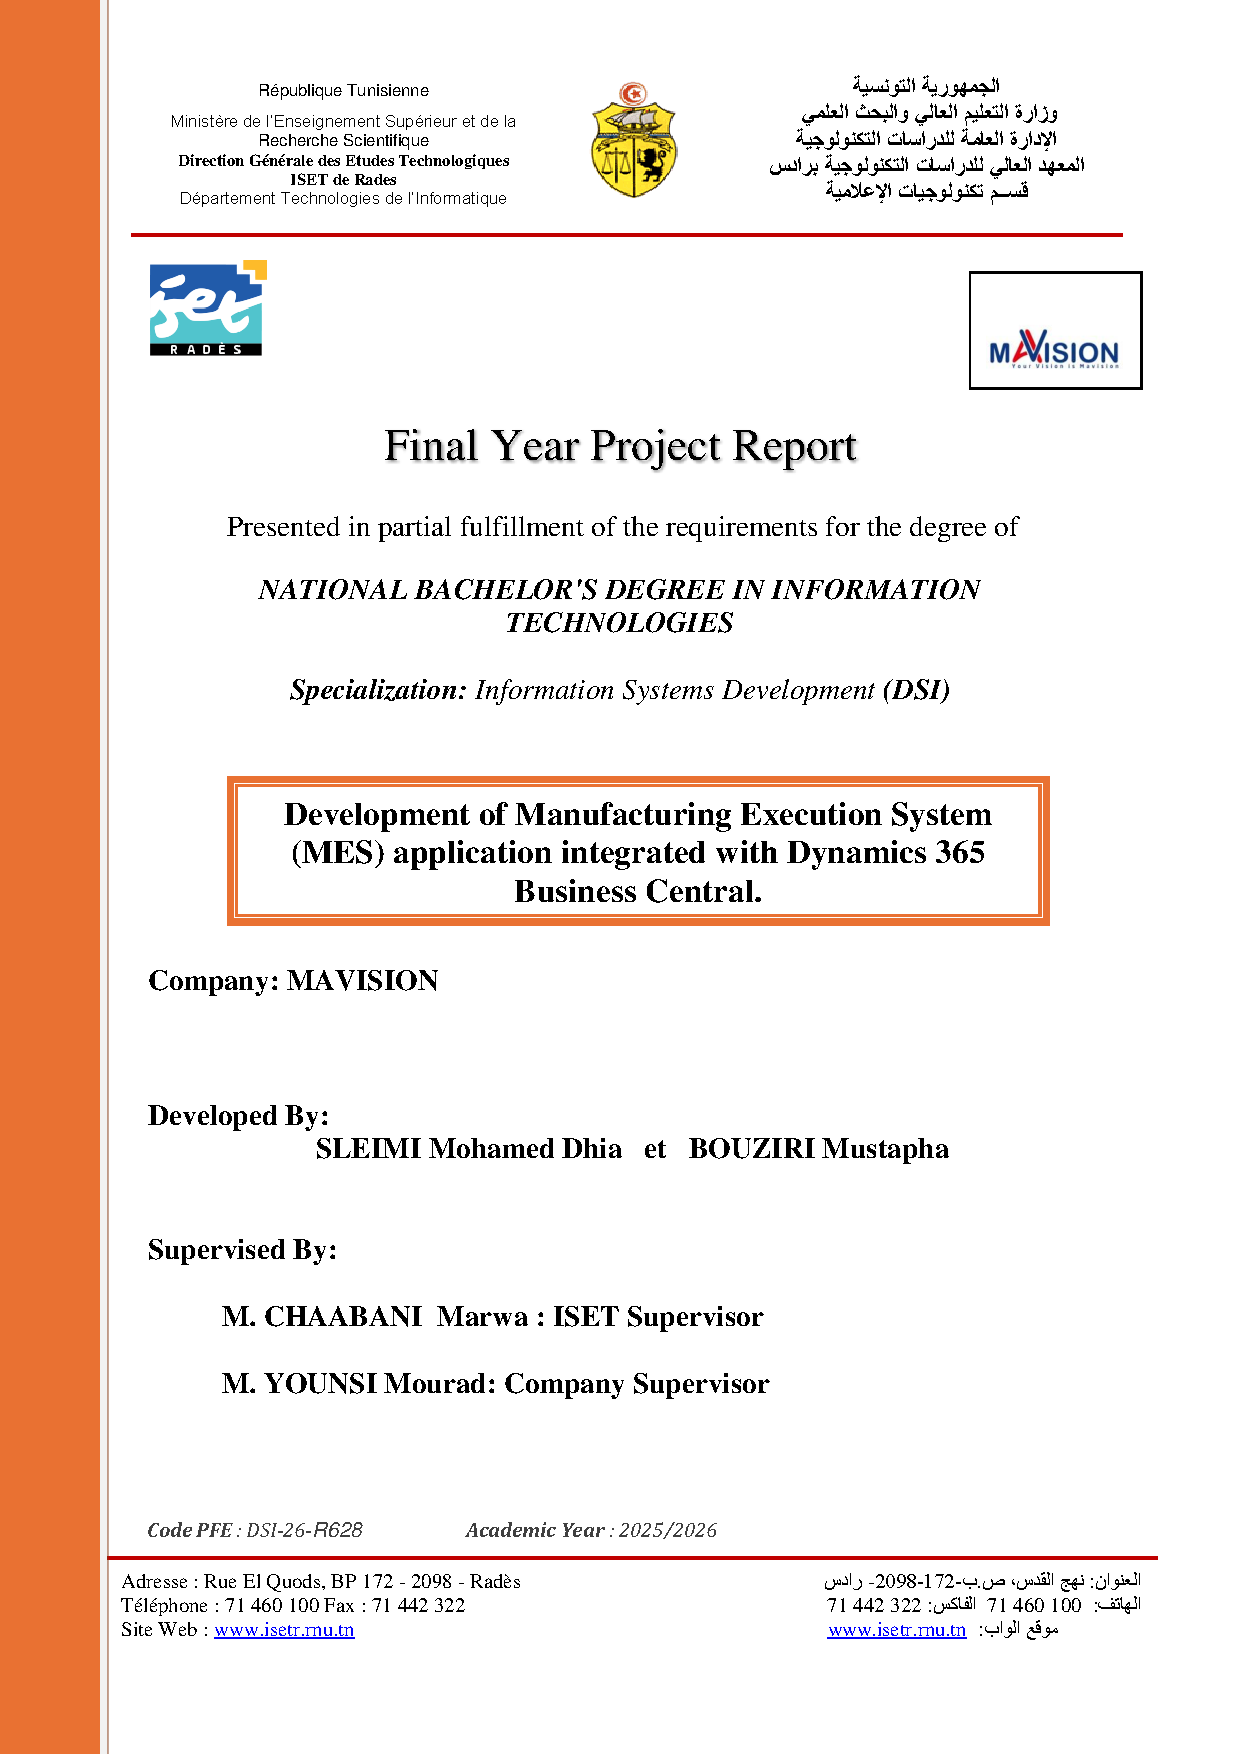
\includepdf[pages=1]{./media/Page-de-garde_DSI-english.pdf}



\cleardoublepage
\thispagestyle{empty}
\begin{center}{\large\bfseries Abstract}\end{center}
\noindent\textbf{Français:} \\[2pt]
Un Système d'Exécution de la Fabrication intégré à Microsoft Dynamics 365 Business Central, 
développé lors d'un stage de quatre mois chez MAVISION. Le système fait le lien entre les ateliers
fonctionnant sur papier et une visibilité en temps réel grâce à quatre couches : une extension AL 
avec des endpoints OData V4, un proxy d'authentification Node.js, une application Flutter 
multiplateforme, et un agent IA Python FastAPI pour les requêtes en langage naturel. Les 
opérateurs et superviseurs gèrent la surveillance des machines, le suivi des nomenclatures, 
la lecture de codes-barres, le signalement des rebuts et l'impression d'étiquettes ; les 
administrateurs gèrent les utilisateurs, les codes-barres et un journal d'audit. Support 
trilingue (anglais, français, arabe) avec mise en page RTL automatique, livré en cinq sprints 
Scrum. \\[2pt]
\textbf{Mots-clés:} MES, Système d'Exécution de la Fabrication, Business Central, Flutter, OData V4,
Intégration ERP, Industrie 4.0, Suivi de Production, Scrum. \\[2pt]
\noindent\textbf{English:} \\[2pt]
A Manufacturing Execution System integrated with Microsoft Dynamics 365 Business Central, built 
during a four-month internship at MAVISION. The system bridges paper-based shop floors with 
real-time visibility through four layers: an AL extension with OData V4 endpoints, a Node.js 
authentication proxy, a cross-platform Flutter app, and a Python FastAPI AI agent for natural-language 
queries. Operators and supervisors handle machine monitoring, BOM tracking, barcode scanning, 
scrap reporting, and label printing; admins manage users, barcodes and an audit log. Trilingual 
support (English, French, Arabic) with automatic RTL layout, delivered across five Scrum sprints. \\[2pt]
\textbf{Keywords:} MES, Manufacturing Execution System, Business Central, Flutter, OData V4,
ERP Integration, Industry 4.0, Production Tracking, Scrum. \\[0pt]
\begin{Arabic}
  \begin{RTL}
    \textbf{العربية:} \\[2pt]
    نظام تنفيذ التصنيع مدمج مع Microsoft Dynamics 365 Business Central، تم تطويره خلال تدريب مدته أربعة أشهر في شركة MAVISION. يربط النظام بين بيئات العمل الورقية في المصانع والرؤية الفورية في الوقت الحقيقي من خلال أربع طبقات: امتداد AL مع نقاط نهاية OData V4، وبروكسي مصادقة Node.js، وتطبيق Flutter متعدد المنصات، ووكيل ذكاء اصطناعي بـ Python FastAPI للاستعلامات باللغة الطبيعية. يتولى المشغلون والمشرفون مراقبة الآلات وتتبع قوائم المواد ومسح الباركود والإبلاغ عن الهدر وطباعة الملصقات؛ فيما يدير المسؤولون المستخدمين والباركود وسجل المراجعة. يدعم النظام ثلاث لغات (الإنجليزية، الفرنسية، العربية) مع تخطيط تلقائي من اليمين إلى اليسار، وقد تم تسليمه عبر خمسة سبرينتات Scrum. \\[2pt]
    \textbf{الكلمات المفتاحية:} نظام تنفيذ التصنيع، Business Central، Flutter，
    OData V4، تكامل ERP، الصناعة 4.0، تتبع الإنتاج، Scrum.
  \end{RTL}
\end{Arabic}
\newpage
\newpage
\newpage

%── ─ Dédicaces ────────────────────────────────────────────────────────────────
\begingroup
\titlespacing*{\chapter}{0pt}{-50pt}{12pt}
\chapter*{Dedication}
\endgroup

\vspace{12pt}
\itshape
\textbf{To my parents}\\[0.1em]
Who have always encouraged me in my studies. Their unconditional love and
their sacrifices have been a constant source of inspiration for me. I am
grateful to have had their support throughout this journey.\\


\vspace{0.1em}
\textbf{To my family}\\[0.1em]
For the efforts you have made to support me throughout my studies.\\


\vspace{0.1em}
\textbf{To my project partner}\\[0.1em]
Your collaboration and invaluable support have been essential\\
to our shared success.\\


\vspace{0.1em}
\textbf{To all my friends}\\[0.1em]
Their sincere friendship, presence and support have made this experience\\
even more enjoyable and meaningful.\\
\vspace{1em}
\begin{flushright}
\normalfont\textit{SLEIMI Mohamed Dhia}
\end{flushright}

\vspace{2em}
\itshape
\textbf{To my family}\\[0.1em]
For your love, patience, and constant support, which have been 
my greatest source of strength throughout this journey.\\

\vspace{0.1em}
\textbf{To my friends}\\[0.1em]
For your encouragement, understanding, and motivation during this experience.\\

\vspace{0.1em}
\textbf{To my teammate}\\[0.1em]
For your collaboration, effort, and commitment, which were essential 
to the success of this project.\\
\vspace{1em}
\begin{flushright}
\normalfont\textit{BOUZIRI Mustapha}
\end{flushright}
\newpage


%─Acknowledgements────────────────────────────────────────────────────────
\chapter*{Acknowledgements}
\markboth{Acknowledgements}{}

First and foremost, We would like to thank our academic supervisor,
\textbf{Ms.~\texttt{CHAABANI Marwa}}, for their expert guidance and
unwavering commitment. Their in-depth knowledge, availability and unconditional support
have been of paramount importance in the completion of this project.

We would also like to express our gratitude to our professional supervisor at
\textbf{MAVISION}, \textbf{Mr.~\texttt{YOUNSI Mourad}}. Their
contribution to this project, both on a technical and organisational level, has been
invaluable. Their strategic vision, domain expertise and availability greatly facilitated
our progress and allowed us to gain an enriching professional experience.

\newpage

\setcounter{page}{1}
% ── Global Table of Contents ────────────────────────────────────────────────

\setcounter{tocdepth}{3}
\tableofcontents
\newpage

% ── List of Tables ──────────────────────────────────────────────────────────
{
  \setlength{\cftbeforelottitleskip}{0pt}
  \setlength{\cftafterlottitleskip}{10pt}
  \listoftables
}
\newpage
% ── List of Figures ─────────────────────────────────────────────────────────
{
  \setlength{\cftbeforeloftitleskip}{0pt}
  \setlength{\cftafterloftitleskip}{10pt}
  \listoffigures
}
\newpage


\chapter*{List of Abbreviations}
\markboth{List of Abbreviations}{}
\begin{longtable}{@{} P{0.18\linewidth} P{0.78\linewidth} @{}}
  \toprule
  \textbf{Abbreviation} & \textbf{Definition} \\
  \midrule
  \endfirsthead
  \toprule \textbf{Abbreviation} & \textbf{Definition} \\ \midrule
  \endhead
  \endlastfoot
  AL      & Application Language (Microsoft Dynamics 365 Business Central) \\
  API     & Application Programming Interface \\
  AI      & Artificial Intelligence \\
  BOM     & Bill of Materials \\
  ERP     & Enterprise Resource Planning \\
  BI      & Business Intelligence \\
  CORS    & Cross-Origin Resource Sharing \\
  GUID    & Globally Unique Identifier \\
  HTTP    & Hypertext Transfer Protocol \\
  JSON    & JavaScript Object Notation \\
  KPI     & Key Performance Indicator \\
  LLM     & Large Language Model \\
  MES     & Manufacturing Execution System \\
  OData   & Open Data Protocol \\
  PDF     & Portable Document Format \\
  QR      & Quick Response (code) \\
  REST    & Representational State Transfer \\
  RTL     & Right-to-Left \\
  SaaS    & Software as a Service \\
  SCRUM   & (no acronym — Scrum is a proper noun) \\
  SHA-256 & Secure Hash Algorithm 256-bit \\
  SSPI    & Security Support Provider Interface \\
  TOTP    & Time-based One-Time Password \\
  TTL     & Time To Live \\
  URL     & Uniform Resource Locator \\
  UML     & Unified Modelling Language \\
  UTC     & Coordinated Universal Time \\
  XML     & Extensible Markup Language \\
  2FA     & Two-Factor Authentication \\
  \bottomrule
\end{longtable}
\newpage

% ---------------------------------------------------------------------------
% GENERAL INTRODUCTION — arabic pagination starts here
% ---------------------------------------------------------------------------
\pagenumbering{arabic}
\setcounter{page}{1}

\chapter*{General Introduction}
\addstarredchapter{General Introduction}
\markboth{General Introduction}{}

In an industrial context undergoing rapid digital transformation, manufacturing
companies face the necessity of optimising their production processes, reducing
downtime and ensuring complete traceability of workshop operations.
\textit{Manufacturing Execution System} (MES), represent a direct response to 
these challenges by bridging the gap between decision-making layers 
\textit{Enterprise Resource Planning} (ERP) and  the production floor.

It is within this context that the present end-of-studies project was carried out at
\textbf{MAVISION}. The project consists of the design and development of an integrated
MES system, structured around two main components: a business back-end developed in
AL language on the Microsoft Dynamics 365 Business Central platform, and a
cross-platform mobile/web application developed with the Flutter framework. The system
enables machine management, production order tracking, real-time production reporting,
as well as user and role-based access management.

This report is structured into several chapters. The first chapter introduces the
host organisation and presents the general framework of the project, highlighting the
limitations of existing solutions and the relevance of the proposed solution. The
second chapter focuses on requirements analysis and specification, as well as the
technology choices made. The subsequent chapters trace the various development phases,
exploring the conceptual aspects and illustrating the results obtained at the end of
each sprint.

Through this approach, we aim to demonstrate how a well-designed digital solution can
transform workshop production management by providing visibility, responsiveness and
performance, serving both operators and management alike.

%% CHAPTERS:BEGIN

% ---------------------------------------------------------------------------
% Global Project Context
% ---------------------------------------------------------------------------
\chapter{Global Project Context}
\graphicspath{{./media/MES_chapter-1-repport/}}
\minitoc
\newpage
\section*{Introduction}
\addcontentsline{toc}{section}{Introduction}

This first chapter serves to contextualise our project. It begins with a brief
introduction to the host organisation, then describes the objectives to be achieved,
provides an in-depth analysis of the existing situation, and finally describes the
methodology used to implement this work.

% ── 1.1 ─────────────────────────────────────────────────────
\section{Presentation of the Host Company}

To properly organise this section, we begin with some general details about
Mavision before addressing the activities directly relevant to us.

\noindent
\begin{minipage}[t]{0.6\textwidth}
	\vspace{0pt}
	\subsection{Overview of Mavision}
		 
	Founded in 2014 and headquartered in Manar~II, Tunis, Mavision~\cite{mavision} is a
	software development company specialising in consulting, auditing and implementing ERP
	information systems. Mavision supports companies in
	their IT development projects and helps its clients better organise themselves around
	their information systems. In addition to its ERP offerings, Mavision develops and
	integrates reporting solutions to help its clients manage
	their business activities more effectively. In order to build lasting trust, Mavision
	places emphasis on its professionalism, commitment and the technical and functional
	expertise of its team.
\end{minipage}
\hfill
\begin{minipage}[t]{0.38\textwidth}
	\vspace{0pt}
	\centering
	
\includegraphics[width=\linewidth]{./media/MES_chapter-1-repport/mavision_logo.jpg}
	\captionof{figure}{Mavision Logo \textnormal{\small  [Source: Mavision, \url{https://www.mavision.tn}, visited April 2025]}}
	\label{fig:mescha-logo_mavision}
\end{minipage}


\subsection{Areas of Expertise}
 
Mavision's activities are structured around three main areas:
 
\textbf{ERP Integration:} Consulting, implementation and integration of ERP solutions,
with a strong focus on Microsoft Dynamics 365 Business Central, as well as project and
platform management, architecture and custom business software design.
 
\textbf{Business Intelligence:} Design and deployment of BI solutions enabling clients
to gain strategic visibility over their operations through dashboards, reporting tools
and data analysis.
 
\textbf{Web \& Mobile Technology:} Development and integration of mobile phone
applications and web platforms that complement ERP systems, enabling clients to manage
their business activities with greater agility and efficiency.

% IMAGE PLACEHOLDER - replace with a photo of the headquarters or premises
\begin{figure}[H]
	\centering
	\missingfigure{Photo of Mavision headquarters / premises}
	\caption{Mavision Headquarters}
	\label{fig:mescha-siege_mavision}
\end{figure}

% ── 1.2 ─────────────────────────────────────────────────────
\section{Project Framework}

This project forms part of our end-of-studies internship, an essential step for
obtaining the \texttt{bachelor's} degree at the
\texttt{Higher Institute of Technological Studies}.
This internship, lasting \texttt{four months}, took place from
\texttt{February 2\textsuperscript{nd}} to \texttt{May 30\textsuperscript{th}} at Mavision. During
this period, we were assigned to the development team.

This team is responsible for designing and maintaining software solutions that meet
the company's business needs, leveraging modern technologies such as Microsoft
Dynamics 365 Business Central and Flutter, and agile practices. Within this context,
we worked on the development of the MES (\textit{Manufacturing Execution System})
project, a mobile and web solution enabling intelligent management of machines and
production operations on the workshop floor.

% ── 1.3 ─────────────────────────────────────────────────────
\section{State of the Art}

\subsection{Subject Overview}

With the rise of Industry 4.0 and the widespread adoption of ERP systems in
manufacturing companies, the need to connect decision-making levels with floor
operations has become critical. A MES (\textit{Manufacturing Execution System}) is
an information system that provides this link in real time: it supervises the
execution of production orders, monitors machine status, records production
declarations and provides operators and supervisors with a consolidated view of
the workshop.

In this context, our project reflects a desire to provide Mavision and its industrial
clients with a MES solution natively integrated with Microsoft Dynamics 365 Business
Central. The primary objective is to allow operators to start and monitor their
production operations from an intuitive mobile/web application, while ensuring data
consistency with the ERP.

\subsection{Problem Statement}

The problem of optimising production floor operations arises with particular force in
manufacturing companies that rely on an ERP system such as Microsoft Dynamics 365
Business Central. Indeed, while Business Central effectively handles production
planning and order management at the decision-making level, no unified, intelligent and
dynamic solution exists to bridge the gap between the ERP and the shop floor in real
time.

This gap leads to several consequences: inability to track the progress of production
orders as they are being executed, manual entry of production declarations through
paper routing sheets or spreadsheet files, lack of visibility for supervisors and
managers on machine states and operation statuses, and insufficient traceability of
actual shop-floor activity. Thus, a central question arises: how can Mavision provide
its industrial clients with a solution that optimises the management of production
operations, ensuring effective, accurate and real-time synchronisation between the shop
floor and the ERP system?

\subsection{Study of the Existing Situation}

Following an in-depth analysis, it is clear that there is a genuine need within
manufacturing companies for a centralised solution to efficiently manage production
operations directly from the workshop floor.

Currently, production tracking is often carried out manually, via paper route sheets
or spreadsheet files, leading to data entry errors, delays in information reporting
and the absence of reliable traceability.

Supervisors and production managers have no real-time visibility into the progress of
production orders, nor the current status of machines (running, paused, out of order).
There is often no tool to automatically correlate production declarations with orders
planned in the ERP.

\subsection{Critical Analysis of the Existing Situation}

In the context of this study, we briefly analysed the MES solution proposed by
Delmia Apriso, one of the leading enterprise-grade Manufacturing Execution Systems
on the market, whose interface is illustrated in the figure below.

Delmia Apriso is a comprehensive cloud-based MES platform developed by Dassault
Systemes, designed for large-scale industrial enterprises.  It covers the full spectrum
of manufacturing operations including production execution, quality management,
labour tracking and supply chain integration. While technically mature and feature-rich, 
it targets large multinational manufacturers with complex and highly customised
deployments, resulting in significant licensing, implementation and maintenance costs
that place it out of reach for small and medium-sized manufacturers.  
 
\begin{figure}[H]
	\centering
	
\includegraphics[width=0.4\linewidth]{./media/MES_chapter-1-repport/logo_delmia_apriso.jpg}
	\caption{Logo of the Delmia Apriso solution \textnormal{\small [Source: Dassault Systèmes, \url{https://www.3ds.com/products/delmia/apriso}, visited April 2025]}}
	\label{fig:mescha-solution_existante}
\end{figure}


From Mavision's perspective as a software provider, the goal is not to use an MES
solution internally, but to deliver one to its industrial clients. The solution must
therefore be cost-effective to sell, straightforward to deploy and maintain at client
sites, and natively integrated into Microsoft Dynamics 365 Business Central, which is
already Mavision's core ERP offering. A heavyweight platform such as Delmia Apriso,
which requires a separate infrastructure and lengthy implementation cycles, is
incompatible with this commercial model. Table~\ref{tab:mescha-comparaison_existant}
summarises the key attributes of Delmia Apriso against the specific needs of the
project.

\begin{longtable}{@{}P{0.38\linewidth}P{0.28\linewidth}P{0.28\linewidth}@{}}
	\caption{Comparison table with Delmia Apriso}
	\label{tab:mescha-comparaison_existant} \\
	\toprule
	\textbf{Features}                               & \textbf{Project needs} & \textbf{Delmia Apriso}     \\
	\midrule
	\endfirsthead
	
	\toprule
	\textbf{Features}                               & \textbf{Project needs} & \textbf{Delmia Apriso}     \\
	\midrule
	\endhead
	
	  
	\multicolumn{3}{r}{\small Continued on next page} \\
	\endfoot
	
	\endlastfoot
	
	Real-time production order tracking             & Yes                    & Yes                        \\ \midrule
	Machine status management                       & Yes                    & Yes                        \\ \midrule
	Production declaration from mobile              & Yes                    & Partial                    \\ \midrule
	Native Business Central integration             & Yes                    & No                         \\ \midrule
	Cross-platform mobile interface                 & Yes                    & Partial                    \\ \midrule
	Role management (Admin / Supervisor / Operator) & Yes                    & Yes                        \\ \midrule
	Secure token-based authentication               & Yes                    & Yes                        \\ \midrule
	Adaptability to internal needs                  & High (custom solution) & Low (proprietary platform) \\ \midrule
	Ease of deployment at client sites              & High                   & Low                        \\ \midrule
	Compatible with SME commercial model            & Yes                    & No                         \\ \bottomrule
\end{longtable}

\subsection{Proposed Solution}

The diagnosis of the current situation has highlighted several shortcomings and
limitations, as detailed in the previous section. To address these, we propose to
design and deploy an innovative MES solution natively integrated with Microsoft
Dynamics 365 Business Central.

This solution consists of two complementary parts:

\begin{itemize}
	\item \textbf{An AL back-end (Business Central)}: developed in AL language, it
	      exposes OData V4 endpoints enabling user management, token-based authentication,
	      machine and operation tracking, as well as production declaration.
	\item \textbf{A Flutter application (front-end)}: a cross-platform mobile and web
	      application allowing operators and supervisors to view production orders assigned to
	      their machine, start, pause or complete an operation, declare produced quantities,
	      and visualise progress in real time.
\end{itemize}

The objective is to optimise every phase of production management by establishing a
reliable, traceable and ergonomic digital framework, serving both operators and
management.

\subsection{Objectives}

Our MES solution aims to:

\begin{itemize}
	\item Provide real-time tracking of machine status and production operations directly
	      from the Business Central ERP.
	\item Allow operators to start, pause and complete operations from an intuitive
	      reactive interfaces.
	\item Record production declarations (produced quantities, scrap) and synchronise
	      them with production orders in Business Central.
	\item Manage users by roles (Administrator, Supervisor, Operator) with secure
	      token-based authentication.
	\item Offer supervisors a consolidated view of production progress across their
	      work centres.
	\item Reduce manual data entry and the risk of errors associated with paper-based
	      or non-integrated processes.
	\item Provide an extensible architecture, ready to accommodate new features
	      (alerts, direct machine connection, etc.).
\end{itemize}

\subsection{Adopted Methodology}

The development method corresponds to an ordered and structured sequence of project
phases, for efficient and optimal management.

\subsubsection{Selection of the Agile Methodology}

Agile is an iterative and collaborative working method that takes into account the
initial needs of the client and any changes that may arise. Its central ingredient is
customer-centred iterative development, which allows a team to gather client feedback
on a regular basis and make the necessary adjustments at the right time.

Thus, the client has a better overview of work progress, leading to regular sessions
that guarantee the delivery of a functional application at all times throughout the
improvement cycles. Consequently, the underlying key idea is to work faster in order
to satisfy a client.

\subsubsection{Adoption of the Scrum Framework}

We adopted the Scrum framework, an agile approach based on short sprints and regular
ceremonies. This choice allowed us to deliver functional increments at the end of each sprint, while maintaining smooth communication with the professional and 
our academic supervisors.

% IMAGE PLACEHOLDER - Scrum cycle diagram
\begin{figure}[H]
	\centering
	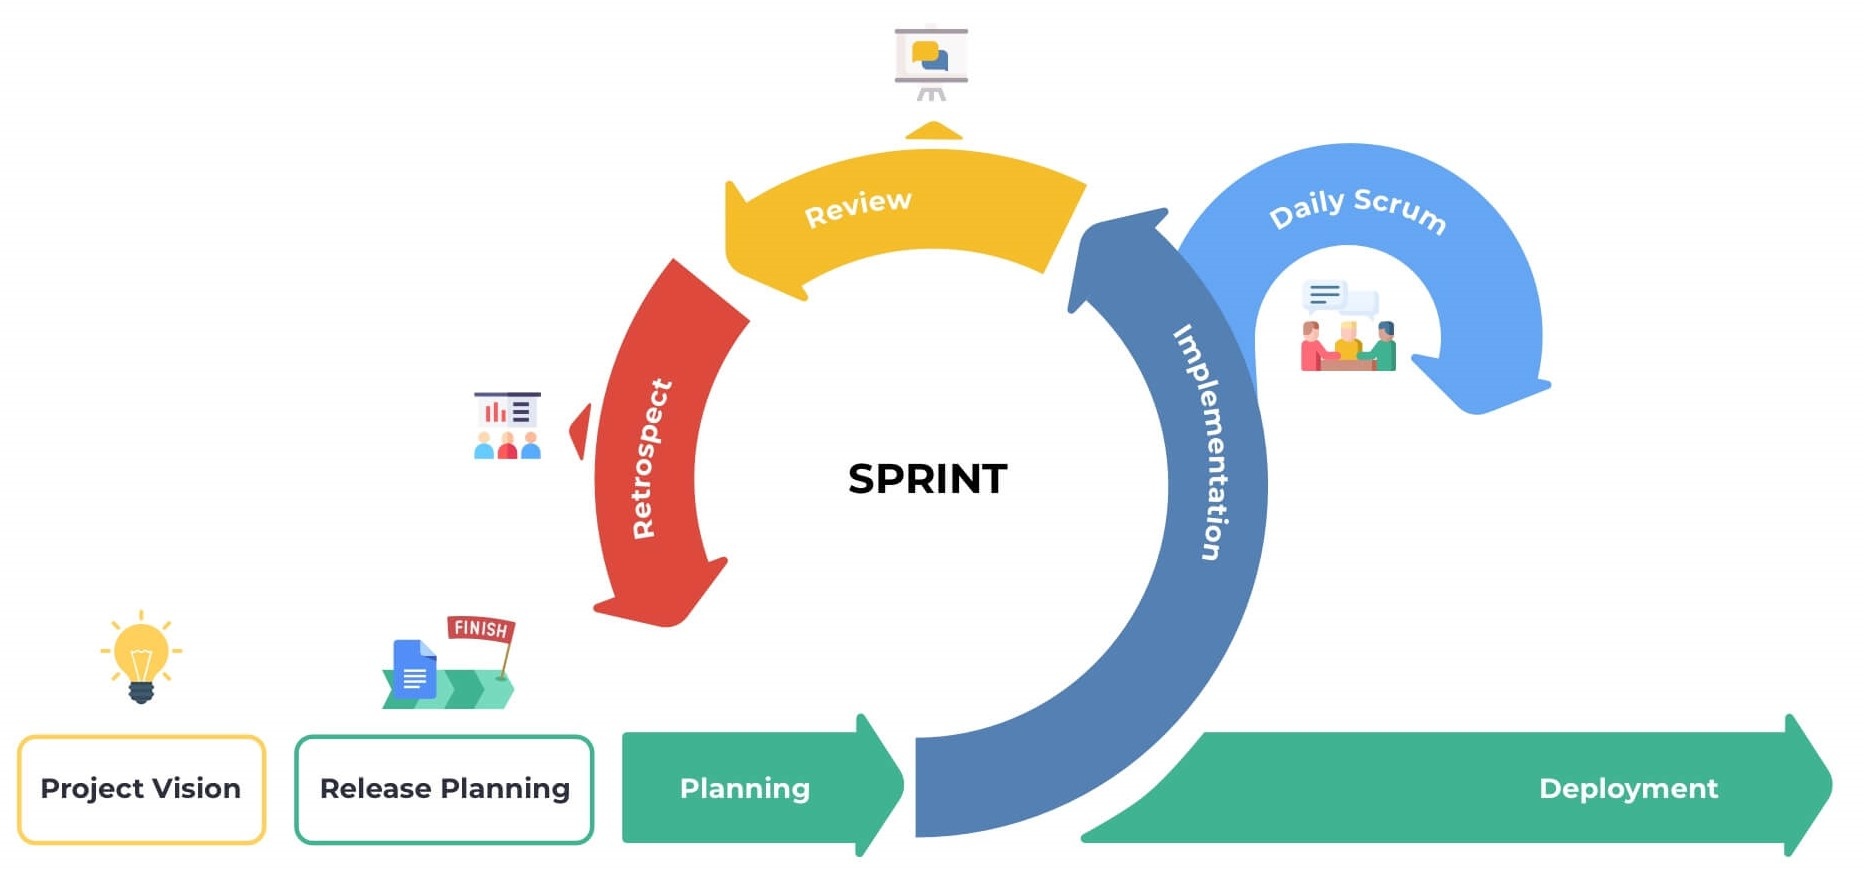
\includegraphics[width=\linewidth,keepaspectratio]{./media/MES_chapter-1-repport/scrum-cycle.jpg}
	\caption{Adopted Scrum development cycle}
	\label{fig:mescha-scrum_cycle}
\end{figure}

\phantomsection
\section*{Conclusion}
\addcontentsline{toc}{section}{Conclusion}

In this chapter, we presented Mavision, the company where the project is being
carried out. We then defined the subject context, as well as the objectives of our
work and the chosen methodology. In order to ensure the report progresses logically,
we will examine the existing solutions used in the company. We will then explain the
functional and non-functional requirements of our solution. This will allow us to
evaluate existing solutions and identify the weaknesses and strengths for which we
should make improvements to our solution. Finally, we will formulate the specific
requirements for our solution.

	
% ============================================================
	
	
% ============================================================
%  BIBLIOGRAPHY
% ============================================================


% ---------------------------------------------------------------------------
% Requirements Analysis and Specification
% ---------------------------------------------------------------------------
\chapter{Requirements Analysis and Specification}
\graphicspath{{./media/MES_chapter-2-repport/}}
\minitoc
\newpage
\section*{Introduction}
\addcontentsline{toc}{section}{Introduction}

Requirements analysis and specification is a crucial phase in the information system
development process. It consists, first and foremost, of clarifying the functional
and non-functional requirements of the system. This step then allows a complete
understanding of the subject in order to position oneself clearly, precisely and
without ambiguity.

% ── 2.1 ─────────────────────────────────────────────────────────────────────
\section{Requirements Analysis}

This step allows us to understand the overall context of our project, that is to say
to identify the main features and determine the actors who will interact with the
system.

\subsection{Identification of Actors}

Actors are entities external to the system (people, hardware, systems) that are
likely to exchange information with it. The following is a list of the actors who
will interact with our system:

\begin{longtable}{@{}P{0.21\linewidth}P{0.75\linewidth}@{}}
	\caption{List of MES application users}
	\label{tab:mescha-acteurs} \\
	\toprule
	\textbf{Actor} & \textbf{Description} \\
	\midrule
	\endfirsthead

	\toprule
	\textbf{Actor} & \textbf{Description} \\
	\midrule
	\endhead

	\multicolumn{2}{r}{\small Continued on next page} \\
	\endfoot

	\endlastfoot

	Administrator  &
	This is the person responsible for the MES platform. They manage all users
	(supervisors, operators), passwords and account statuses. They have access to all
	administration application dashboards. \\[6pt]

	Supervisor     &
	This is an intermediate user. They can monitor the progress of production operations
	on their work centre, view machine status and track the progress of production
	orders. Mark operation as finished or cancel/interupt uneeded operations. 
	View machine dashboards. Have access to all the access of the operators \\[6pt]

	Operator       &
	This is the end user of the MES application. Assigned to a work centre
	(\textit{Work Center}), they can view the production orders assigned to their machine,
	start, pause or resume an operation, declare produced quantities, declare defective 
	material, and scan components for consumption. \\

\end{longtable}

\subsection{Identification of Requirements}

At this stage, we will define the specific requirements of our
application, clearly distinguishing functional requirements from non-functional
requirements.

\subsubsection{Functional Requirements}

Each actor of the platform has specific expectations referred to as functional
requirements. To define the functional scope, it is necessary that the conceptual
solution meets these functional requirements.

\begin{itemize}
	\item \textbf{Authentication}: This feature allows any user to log in to the
	      platform using their Auth~ID and password. Upon first login, the user is prompted
	      to change their temporary password. A secure session token (GUID, 12~h validity) is
	      issued upon each successful login.

	\item \textbf{Two-Factor Authentication (2FA)}: When enabled globally by the
	      administrator, users must complete a second authentication step by scanning their
	      personal badge QR~code after entering their credentials. Administrators can view,
	      print, and regenerate badge secrets for any user.

	\item \textbf{Application Setup}: On first launch, the user must configure the
	      middleware host URL (entered manually or obtained by scanning a QR~code) so that
	      the application connects to the correct server instance. The host is persisted
	      across sessions and can be changed from the login page.

	\item \textbf{User Management}: This feature allows the administrator to:
	      \begin{itemize}
	      	\item View the complete list of MES users.
	      	\item Create a new user account by linking it to a Business
	      	      Central employee and assigning them a role and work centre(s) if needed.
	      	\item Generate and assign a temporary password.
	      	\item Activate or deactivate an account (automatic revocation of active tokens).
	      	\item Change a user's role (Operator, Supervisor, Administrator) and work centre assignment.
	      	\item View, print, and regenerate a user's badge QR~code for 2FA purposes.
	      \end{itemize}

	\item \textbf{Security Policy}: The administrator can configure a password rotation
	      period (in days). A scheduled background job runs every 24~hours and flags users
	      whose password age exceeds the configured period, forcing them to change their
	      password on next login.

	\item \textbf{Machine Management}: This feature allows users to:
	      \begin{itemize}
	      	\item View the list of machines in a work centre with their current status
	      	       (Idle, Working).
	      	\item View the production order currently running on each machine.
	      \end{itemize}

	\item \textbf{Production Order Management}: This feature allows the \userrole{Operator} and the \userrole{supervisor} to:
	      \begin{itemize}
	      	\item View production orders (Planned, Firm, Released) assigned to their machine.
	      	\item Filter and sort orders by status or date.
	      	\item View the details of an order (item, quantity, planned dates, operation
	      	      description).
	      \end{itemize}

	\item \textbf{Production Operation Management}: This feature is the core of the
	      system. It allows the operator or Supervisor to:
	      \begin{itemize}
	      	\item Start an operation (validation of prerequisites: released order, free machine, previous operation completed if applicable).
	      	\item Pause or resume an ongoing operation.
		 	\item Declare produced quantities (validation: quantity $> 0$, no excess of the ordered quantity).
	      	\item View progress in real time (produced quantity, completion percentage, operation status, scrapped units).
			\item View the Bill of Materials for the current operation with component consumption
	      	\item Report scrapped units with a reason code.
	      	\item scan components into the operation to record consumption against the BOM.
	      \end{itemize}

	\item \textbf{Progress Dashboard}: Allows the operator and supervisor to view all
	      active operations (Running / Paused) on a given machine, with their respective
	      progress.

	\item \textbf{Password Change}: Allows any logged-in user to change their password
	      by entering their old password and the new one.

	\item \textbf{AI Chat Assistant}: An embedded natural-language assistant allows
	      operators and supervisors to query machine status, production progress, scrap
	      data, BOM, and history without navigating the full interface. The assistant
	      resolves ambiguous machine references, answers fleet-wide questions, surfaces
	      operational anomalies, and provides contextual navigation shortcuts.
\end{itemize}

\subsubsection{Non-Functional Requirements}

To define the non-functional scope, it is necessary that the conceptual solution meets
these non-functional requirements:

\begin{itemize}
	\item \textbf{Performance}: The platform performs efficiently in terms of handling
	      routine operations (login, order consultation, production declaration).

	\item \textbf{Security}: Implementation of a token-based authentication system
	      (signed GUID, 12~h expiry) and role management (Admin, Supervisor, Operator) to
	      control access to features. Passwords are stored as SHA-256 hashes with a salt.
	      Optional two-factor authentication enforces badge QR verification as a second
	      factor. A configurable password expiry policy forces periodic credential rotation.

	\item \textbf{Maintainability}: The AL back-end code is organised in layers
	      (Tables, Enums, Codeunits, API Pages) and the Flutter code follows a layered
	      architecture (Data, Domain, Presentation) with the Provider pattern, facilitating
	      updates and the addition of new features.

	\item \textbf{Ergonomics}: The user interface is adaptive (mobile, tablet, PC)
	      thanks to responsive layouts dedicated to each form factor, minimising the learning
	      curve for workshop operators.

	\item \textbf{Portability}: The Flutter application is compiled for Android, iOS,
	      Web, Linux, macOS and Windows from a single codebase. The Business Central back-end
	      is deployable both on-premises and in SaaS (cloud) mode.
\end{itemize}

% ── 2.2 ─────────────────────────────────────────────────────────────────────
\section{Project Management with Scrum}

\subsection{Backlog Features}

% ===================== DOMAIN 1: AUTHENTICATION & USER MANAGEMENT =====================
\subsubsection{Domain 1: Authentication \& User Management}
\label{domain1}

\vspace{0.3cm}

\begin{longtable}{p{1.5cm} p{5cm} p{6.5cm} p{2cm}}
	\hline
	\textbf{ID} & \textbf{User Story} & \textbf{Acceptance Criteria} & \textbf{Priority} \\
	\hline
	\endfirsthead

	\hline
	\textbf{ID} & \textbf{User Story} & \textbf{Acceptance Criteria} & \textbf{Priority} \\
	\hline
	\endhead

	\multicolumn{4}{r}{\small Continued on next page} \\
	\endfoot

	\endlastfoot

	\textbf{US-1.1} &
	As an \userrole{Administrator}, I need to assign a user account for each employee  so
	that users only access features appropriate to their role.
	& \begin{itemize}[noitemsep, topsep=0pt, partopsep=0pt, leftmargin=*]
	\item Ability to assign a user as \userrole{Operator} or \userrole{Supervisor} or \userrole{Administrator}.
	\item Unauthorized actions are blocked with clear error messages.
	\end{itemize} &
	High \\
	\midrule

	\textbf{US-1.2} &
	As a User (\userrole{Operator} / \userrole{Supervisor} / \userrole{Administrator}),
	I need to log into the system with my credentials so that I can access
	features appropriate to my role.
	&
	\begin{itemize}[noitemsep, topsep=0pt, partopsep=0pt, leftmargin=*]
	\item User can enter username and password.
	\item System validates credentials against the \techname{MES}.
	\item Session token is created upon successful authentication.
	\item User is redirected to the appropriate dashboard based on role.
	\end{itemize} &
	High \\
	\midrule

	\textbf{US-1.3} &
	As an \userrole{Administrator}, I need to search users.
	& \begin{itemize}[noitemsep, topsep=0pt, partopsep=0pt, leftmargin=*]
	\item Ability to filter users based on their role.
	\item Ability to search for a specific user.
	\end{itemize} &
	High \\
	\midrule

	\textbf{US-1.4} &
	As an \userrole{Administrator}, I need to see a list of all
	users with their details so that I can manage their accounts.
	& \begin{itemize}[noitemsep, topsep=0pt, partopsep=0pt, leftmargin=*]
	\item The user list displays each account's full name, email, role, when he was active, and work centre.
	\item Clicking on the action button shows a dropdown menu with available actions(change role, generate password, view badge, and toggle activation).
	\item The list refreshes automatically after a new user is created.
	\end{itemize} & High \\ \midrule

	\textbf{US-1.5} &
	As an \userrole{Administrator}, I need to generate and assign temporary
	passwords to users so that they can log in for the first time.
	& \begin{itemize}[noitemsep, topsep=0pt, partopsep=0pt, leftmargin=*]
	\item Admin can generate a random secure password for any user.
	\item The generated password is sent to the \techname{ERP} via \texttt{AdminSetPassword}.
	\item The target account is flagged \domainterm{Need To Change Password} after the password is set.
	\item Success or failure is reported to the admin with a clear message.
	\end{itemize} & High \\ \midrule

	\textbf{US-1.6} &
	As an \userrole{Administrator}, I need to change the role and work-centre
	assignment of an existing user so that access rights stay current.
	&
	\begin{itemize}[noitemsep, topsep=0pt, partopsep=0pt, leftmargin=*]
	\item Admin can select a new role for any other user.
	\item Work-centre list updates based on the selected role.
	\item All active tokens for the target user are revoked on save.
	\item The user list refreshes after a successful change.
	\end{itemize}
	&
	High \\ \midrule

	\textbf{US-1.7} &
	As an \userrole{Administrator}, I need to activate or deactivate a user
	account so that access can be revoked without deleting the account.
	&
	\begin{itemize}[noitemsep, topsep=0pt, partopsep=0pt, leftmargin=*]
	\item Admin can toggle the active status of any other user.
	\item Deactivation immediately revokes all active tokens.
	\item The user row updates its visual status indicator immediately.
	\end{itemize}
	&
	High \\ \midrule

	\textbf{US-1.8} &
	As a User (\userrole{Operator} / \userrole{Supervisor} / \userrole{Administrator}),
	I need to complete a badge QR code scan after entering my credentials so
	that my identity is verified by a second factor.
	&
	\begin{itemize}[noitemsep, topsep=0pt, partopsep=0pt, leftmargin=*]
	\item \domainterm{2FA} prompt appears only when \domainterm{TwoFA Enabled} is active in \techname{MES Settings}.
	\item Camera opens and scans a QR badge code.
	\item Manual entry field available as a fallback.
	\item Session token is persisted only after successful badge verification.
	\item Failed scan shows an error; scanner reactivates.
	\item User can cancel and return to the login page.
	\end{itemize}
	&
	High \\ \midrule

	\textbf{US-1.9} &
	As an \userrole{Administrator}, I need to view, print, and regenerate a
	user's badge QR~code so that I can distribute it and invalidate a lost or
	compromised badge.
	&
	\begin{itemize}[noitemsep, topsep=0pt, partopsep=0pt, leftmargin=*]
	\item Badge QR rendered from the user's \domainterm{Badge Secret} via a barcode widget.
	\item Print button generates a PDF.
	\item Regenerate action shows a confirmation dialog before replacing the secret.
	\item New QR is displayed immediately after regeneration.
	\end{itemize}
	&
	High \\ \midrule

	\textbf{US-1.10} &
	As an \userrole{Administrator}, I need to globally enable or disable \domainterm{2FA}
	and configure a password rotation period so that I can control the
	organisation's authentication security level.
	&
	\begin{itemize}[noitemsep, topsep=0pt, partopsep=0pt, leftmargin=*]
	\item \domainterm{2FA} toggle and password rotation period field available on a \uilabel{Settings} page.
	\item Changes take effect on the next login attempt.
	\item Settings are persisted.
	\item A scheduled job (every 24~h) flags users whose password age exceeds the configured period.
	\item Unsaved changes display a persistent banner with \uilabel{Discard} and \uilabel{Save} actions.
	\end{itemize}
	&
	High \\ \midrule

	\textbf{US-1.11} &
	As a first-time user, I need to configure the middleware host URL (or scan
	a QR~code) so that the application connects to the correct server instance.
	&
	\begin{itemize}[noitemsep, topsep=0pt, partopsep=0pt, leftmargin=*]
	\item \uilabel{Paring} page shown on first launch when no host is saved.
	\item URL can be entered manually or obtained by scanning a QR~code.
	\item URL is validated (no spaces, no illegal characters).
	\item Saved host persists across app restarts.
	\item \uilabel{Change Host} link on the login page allows re-entering the pairing screen.
	\end{itemize}
	&
	High \\
	\midrule

	\textbf{US-1.12} &
	As an \userrole{Administrator}, I need to export the list of users so that
	I can use the information in other applications or processes.
	& \begin{itemize}[noitemsep, topsep=0pt, partopsep=0pt, leftmargin=*]
	\item The ability to export all user info.
	\item The information is structured in the form of an excel file.
	\end{itemize} &
	Medium \\
	\bottomrule
\end{longtable}


% ===================== DOMAIN 2: MACHINE MONITORING =====================
\subsubsection{Domain 2: Machine \& Production Management}
\label{domain2}

\vspace{0.3cm}

\begin{longtable}{ p{1.5cm} p{5cm} p{6.5cm} p{2cm} }
	\toprule
	\textbf{ID} & \textbf{User Story} & \textbf{Acceptance Criteria} & \textbf{Priority} \\
	\midrule
	\endfirsthead

	\toprule
	\textbf{ID} & \textbf{User Story} & \textbf{Acceptance Criteria} & \textbf{Priority} \\
	\midrule
	\endhead

	\multicolumn{4}{r}{\small Continued on next page} \\
	\endfoot

	\endlastfoot

	\textbf{US-2.1} &
	As an \userrole{Operator} or \userrole{Supervisor}, I need to see the list
	of machines in my work center with their current status so that I can see
	which machines are currently active.
	& \begin{itemize}[noitemsep, topsep=0pt, partopsep=0pt, leftmargin=*]
	\item Machine list is scoped to the authenticated user's work centre.
	\item Each card shows machine name, current status (\domainterm{Idle},
	\domainterm{Working}), active production order number, operation No, item No, and
	the item name.
	\item The list refreshes automatically every 20 seconds.
	\end{itemize} &
	High \\
	\midrule

	\textbf{US-2.2} &
	As an \userrole{Operator} or \userrole{Supervisor}, I need to view the operations of the
	production orders assigned to a machine so that I know what work needs
	to be done.
	& \begin{itemize}[noitemsep, topsep=0pt, partopsep=0pt, leftmargin=*]
	\item Only \domainterm{Planned}, \domainterm{Firm Planned}, or
	\domainterm{Released} orders are shown.
	\item Each card displays order number, item description, planned quantity,
	planned start and end dates, operation description, and operation number.
	\end{itemize} &
	High \\
	\midrule

	\textbf{US-2.3} &
	As an \userrole{Operator} or \userrole{Supervisor}, I need to start a
	production operation so that the system records that the order has begun.
	& \begin{itemize}[noitemsep, topsep=0pt, partopsep=0pt, leftmargin=*]
	\item Only \domainterm{operation} from \domainterm{Released} orders may be started.
	\item An operation cannot be started if it is already running.
	\item A machine cannot run two operations simultaneously.
	\item A new MES Operation State record is created with status change so it can be tracked.
	\item The previous operation in the same production order (if any) must be
	\domainterm{Finished}, \domainterm{Interrupted}, or currently \domainterm{Running}
	with enough send-ahead quantity.
	\end{itemize} & High \\ \midrule

	\textbf{US-2.4} &
	As a \userrole{Supervisor} or \userrole{Operator}, I need to monitor the
	current status of all active operations on a machine so that I can follow
	the progress of each order.
	& \begin{itemize}[noitemsep, topsep=0pt, partopsep=0pt, leftmargin=*]
	\item The Operations Progress tab shows all operations whose latest status
	record is \domainterm{Running} or \domainterm{Paused}.
	\item Each card shows order number, operation number, current status, operation description,
	last updated timestamp, and progress.
	\item Data refreshes automatically every 5 seconds.
	\end{itemize} & High \\ \midrule

	\textbf{US-2.5} &
	As an \userrole{Operator} or \userrole{Supervisor}, I need a tabbed view
	for a machine so that I can navigate between pending orders and active
	operation progress without leaving the machine context.
	& \begin{itemize}[noitemsep, topsep=0pt, partopsep=0pt, leftmargin=*]
	\item Selecting a machine from the list opens a dedicated machine page.
	\item The page provides three tabs: \domainterm{Orders},
	\domainterm{Progress}, and \domainterm{History}.
	\item The active tab is visually highlighted in the navigation bar.
	\end{itemize} & High \\ \midrule

	\textbf{US-2.6} &
	As an \userrole{Operator} or \userrole{Supervisor}, I need to filter and
	sort production orders so that I can quickly find the most relevant work.
	& \begin{itemize}[noitemsep, topsep=0pt, partopsep=0pt, leftmargin=*]
	\item Orders can be searched by order number, item description, or date.
	\item Orders can be filtered by status (\domainterm{All}, \domainterm{Planned},
	\domainterm{Firm Planned}, \domainterm{Released}).
	\item Orders can be sorted by planned start date ascending or descending.
	\item On mobile, the status filter is accessible via a compact popup menu.
	\end{itemize} & High \\ \midrule

	\textbf{US-2.7} &
	As a \userrole{Supervisor} or \userrole{Operator}, I need to view the
	history of completed operations for a machine so that I can audit past
	production.
	&
	\begin{itemize}[noitemsep, topsep=0pt, partopsep=0pt, leftmargin=*]
	\item The History tab shows all operations with status
	\domainterm{Finished},\domainterm{Interrupted}, or \domainterm{Cancelled}.
	\item Each card shows order number, status, product name, produced
	quantity, start time, and end time.
	\item The list supports free-text search and sort by start date.
	\item Tapping a card navigates to the full operation detail page.
	\end{itemize}
	&
	High \\
	\bottomrule
\end{longtable}


\subsubsection{Domain 3: Production Execution \& Traceability}
\label{domain3}

\vspace{0.3cm}

\begin{longtable}{p{1.5cm} p{5cm} p{6.5cm} p{2cm}}
	\hline
	\textbf{ID} & \textbf{User Story} & \textbf{Acceptance Criteria} & \textbf{Priority} \\
	\hline
	\endfirsthead
	\hline
	\textbf{ID} & \textbf{User Story} & \textbf{Acceptance Criteria} & \textbf{Priority} \\
	\hline
	\endhead
	\multicolumn{4}{r}{\small Continued on next page} \\
	\endfoot
	\endlastfoot

	\textbf{US-3.1} &
	As an \userrole{Operator} or \userrole{Supervisor}, I need to declare the
	quantity produced in a cycle so that the system records production progress.
	&
	\begin{itemize}[noitemsep, topsep=0pt, partopsep=0pt, leftmargin=*]
	\item Declared quantity must be positive and not exceed remaining quantity that need to be produced.
	\item Declared quantity must be less than the amount that can be produced with the available components scanned remaining.
	\item Each declaration creates a new progression cycle record.
	\item Produced quantity and progress percentage update immediately.
	\end{itemize}
	& High \\ \midrule

	\textbf{US-3.2} &
	As an \userrole{Operator} or \userrole{Supervisor}, I need to pause and
	resume an active operation so that interruptions are tracked accurately.
	&
	\begin{itemize}[noitemsep, topsep=0pt, partopsep=0pt, leftmargin=*]
	\item A Running operation can be paused; a Paused one can be resumed.
	\item A machine cannot resume if another operation is already running.
	\end{itemize}
	& High \\ \midrule

	\textbf{US-3.3} &
	As a \userrole{Supervisor}, I need to finish, interrupt or cancel an operation so that
	the machine is released and the order is closed in the system.
	&
	\begin{itemize}[noitemsep, topsep=0pt, partopsep=0pt, leftmargin=*]
	\item Finishing a complete order (100\%) shows a green confirmation dialog.
	\item Interrupting or Cancelling an operation shows a red warning dialog.
	\item If the operation is started then it is marked as interrupted otherwise as cancelled
	\item Closing sets the execution end time and inserts an Idle machine status.
	\end{itemize}
	& High \\ \midrule

	\textbf{US-3.4} &
	As an \userrole{Operator} or \userrole{Supervisor}, I need a dedicated
	operation detail page with up-to-date data in one place.
	&
	\begin{itemize}[noitemsep, topsep=0pt, partopsep=0pt, leftmargin=*]
	\item Shows status, order number, product, required and produced quantities.
	\item The information updates automatically without a manual refresh.
	\end{itemize}
	& High \\ \midrule

	\textbf{US-3.5} &
	As an \userrole{Operator} or \userrole{Supervisor}, I need to see all
	production cycles declared for an operation.
	&
	\begin{itemize}[noitemsep, topsep=0pt, partopsep=0pt, leftmargin=*]
	\item Cycle table lists operator, quantity, cumulative total, and timestamp.
	\item Records ordered newest-first with pagination.
	\item Updates after each new declaration.
	\end{itemize}
	& High \\ \midrule

	\textbf{US-3.6} &
	As an \userrole{Operator} or \userrole{Supervisor}, I need a visual chart
	of declarations over time to identify performance trends.
	&
	\begin{itemize}[noitemsep, topsep=0pt, partopsep=0pt, leftmargin=*]
	\item Line chart plots cycle quantity vs.\ declaration time.
	\item Touch tooltip shows operator, quantity, total production, timestamp.
	\item Auto-scrolls to most recent data point on load and refresh.
	\end{itemize}
	& Medium \\ \midrule

	\textbf{US-3.7} &
	As an \userrole{Operator} or \userrole{Supervisor}, I need to see the Bill
	of Materials for an operation to know which components are required.
	&
	\begin{itemize}[noitemsep, topsep=0pt, partopsep=0pt, leftmargin=*]
	\item Components are colour-coded by remaining amount (the needed amount (green) / less then necessary to make a single item (red) otherwise (yellow)).
	\item BOM data refreshes after every consumption event.
	\item can be expanded to a dialog for a better view on larger screens.
	\item search by name and filter by state
	\end{itemize}
	& High \\ \midrule

	\textbf{US-3.8} &
	As an \userrole{Operator} or \userrole{Supervisor}, I need to report
	scrapped units with a reason code so that waste is accurately tracked.
	&
	\begin{itemize}[noitemsep, topsep=0pt, partopsep=0pt, leftmargin=*]
	\item Scrap can only be declared when the operation is Running.
	\item A reason code must be selected before submission.
	\item Need to select either input material or output scrap.
	\item the quantity of scrapped units cannot exceed the quantity 
	that can be produced with the available components scanned remaining.
	\item Each declaration's quantity, code, and operator is stored for tracibility.
	\end{itemize}
	& High \\ \midrule

	\textbf{US-3.9} &
	As a \userrole{Supervisor}, I need to declare production or scrap on behalf of an
	operator so that output is attributed to the correct person.
	&
	\begin{itemize}[noitemsep, topsep=0pt, partopsep=0pt, leftmargin=*]
	\item Supervisor role sees an operator selector in the declare dialog.
	\item Selected operator's ID is stored with the declaration record for tracibility.
	\item If no operator is selected, it is declared as if the supervisor made the declaration.
	\end{itemize}
	& Medium \\ \midrule

	\textbf{US-3.10} &
	As an \userrole{Operator} or \userrole{Supervisor}, I need to scan
	components into an operation so that consumption is recorded against the BOM.
	&
	\begin{itemize}[noitemsep, topsep=0pt, partopsep=0pt, leftmargin=*]
	\item any camera connected to the device reads  barcodes.
	\item Duplicate scan increments quantity on the existing row.
	\item Confirming scans inserts consumption records and refreshes the BOM.
	\item After confirmation, the inventory in the ERP is updated to reflect the consumed quantity.
	\end{itemize}
	& High \\ \midrule

	\textbf{US-3.11} &
	As an \userrole{Operator} or \userrole{Supervisor}, I need to print a label
	for a production order so that produced parts are correctly identified.
	&
	\begin{itemize}[noitemsep, topsep=0pt, partopsep=0pt, leftmargin=*]
	\item Label includes DataMatrix barcode encoding order, machine, item data.
	\item PDF generation supports landscape/portrait toggle.
	\item Print button available only when operation is Finished or progress
	$\geq$ 100\%.
	\end{itemize}
	& Medium \\ \midrule

	\textbf{US-3.12} &
	As an \userrole{Operator} or \userrole{Supervisor}, I need a label printed
	for each declared unit so that individual pieces carry traceable information.
	&
	\begin{itemize}[noitemsep, topsep=0pt, partopsep=0pt, leftmargin=*]
	\item One PDF page per declared unit with a label counter.
	\item Same DataMatrix encoding as the production label.
	\item Launched automatically after a successful production declaration.
	\end{itemize}
	& Medium \\
	\bottomrule
\end{longtable}


% ===================== DOMAIN 4: ADMINISTRATION =====================
\subsubsection{Domain 4: Administration \& Monitoring}
\label{domain4}

\vspace{0.3cm}

\begin{longtable}{p{1.5cm} p{5cm} p{6.5cm} p{2cm}}
	\hline
	\textbf{ID} & \textbf{User Story} & \textbf{Acceptance Criteria} & \textbf{Priority} \\
	\hline
	\endfirsthead
	\hline
	\textbf{ID} & \textbf{User Story} & \textbf{Acceptance Criteria} & \textbf{Priority} \\
	\hline
	\endhead
	\multicolumn{4}{r}{\small Continued on next page} \\
	\endfoot
	\endlastfoot

	\textbf{US-4.1} &
	As an \userrole{Supervisor}, I need a performance dashboard for all
	machines so that I can monitor production health across the facility.
	&
	\begin{itemize}[noitemsep, topsep=0pt, partopsep=0pt, leftmargin=*]
	\item Dashboard shows uptime, operation cancelled or finished count, total produced, and scrap
	per machine.
	\item Configurable time-range (hours back) filter.
	\end{itemize}
	& High \\ \midrule

	\textbf{US-4.2} &
	As an \userrole{Administrator}, I need a filterable activity log
	of all system actions so that I can audit operator and machine activity.
	&
	\begin{itemize}[noitemsep, topsep=0pt, partopsep=0pt, leftmargin=*]
	\item Log entries includes all the relevant fields with timestamps.
	\item Filterable by action type and time range.
	\end{itemize}
	& High \\ \midrule


	\textbf{US-4.3} &
	As any user, I need the application available in English, French, and Arabic
	so that I can use it in my preferred language.
	&
	\begin{itemize}[noitemsep, topsep=0pt, partopsep=0pt, leftmargin=*]
	\item Language selector on login screen and in profile page.
	\item All UI strings externalised; no hard-coded text.
	\item Arabic locale activates RTL layout automatically.
	\item Language preference persisted across sessions in the same device.
	\end{itemize}
	& High \\ \midrule

	\textbf{US-4.4} &
	As a first-time user, I need guided coach-mark tutorials so that I can learn
	the interface without external documentation.
	&
	\begin{itemize}[noitemsep, topsep=0pt, partopsep=0pt, leftmargin=*]
	\item Tutorials shown exactly once per install per screen.
	\item Coach marks cover: machine list, machine detail tabs, operation
	detail, and admin dashboard.
	\item Localised skip button text.
	\end{itemize}
	& Medium \\
	\bottomrule
\end{longtable}


% ===================== DOMAIN 5: AI ASSISTANT =====================
\subsubsection{Domain 5: AI Chat Assistant \& Analytical Intelligence}
\label{domain5}

\vspace{0.3cm}

\begin{longtable}{p{1.5cm} p{5cm} p{6.5cm} p{2cm}}
	\hline
	\textbf{ID} & \textbf{User Story} & \textbf{Acceptance Criteria} & \textbf{Priority} \\
	\hline
	\endfirsthead
	\hline
	\textbf{ID} & \textbf{User Story} & \textbf{Acceptance Criteria} & \textbf{Priority} \\
	\hline
	\endhead
	\multicolumn{4}{r}{\small Continued on next page} \\
	\endfoot
	\endlastfoot

	\textbf{US-5.1} &
	As an \userrole{Operator} or \userrole{Supervisor}, I need a natural-language
	chat assistant so that I can query machine status, production progress, and
	operational data without navigating the full UI.
	&
	\begin{itemize}[noitemsep, topsep=0pt, partopsep=0pt, leftmargin=*]
	\item Chat panel opens as a side overlay on wide screens and as a dialog on mobile.
	\item Assistant answers questions about machines, orders, live operations, BOM,
	history, and scrap.
	\item Responses are scoped to the user's own work centres (access control enforced).
	\item Multi-turn conversation history is maintained within the session.
	\item Conversation can be cleared by the user.
	\end{itemize}
	& High \\ \midrule

	\textbf{US-5.2} &
	As an \userrole{Operator} or \userrole{Supervisor}, I need the assistant to
	resolve ambiguous machine references (e.g.\ ``Fraiseuse~3'') so that I do not
	need to know exact machine codes.
	&
	\begin{itemize}[noitemsep, topsep=0pt, partopsep=0pt, leftmargin=*]
	\item Machine names, partial codes, and digit-only references are matched to
	the correct machine using a five-tier fuzzy resolution strategy.
	\item High-confidence matches ($\geq$ 85\%) are resolved silently.
	\item Low-confidence matches present up to 3 candidates for disambiguation.
	\item Machine access control is enforced after resolution.
	\end{itemize}
	& High \\ \midrule

	\textbf{US-5.3} &
	As an \userrole{Operator} or \userrole{Supervisor}, I need the assistant to
	answer fleet-wide questions (e.g.\ ``which machines are running?'') so that I
	get a consolidated view without visiting each machine individually.
	&
	\begin{itemize}[noitemsep, topsep=0pt, partopsep=0pt, leftmargin=*]
	\item Queries about all machines trigger a parallel fan-out across work centres.
	\item Results are filtered by running / idle / overdue / scrap status as requested.
	\item Fan-out is capped to control response time.
	\item Fleet summary includes machine count, utilisation percentage, and active orders.
	\end{itemize}
	& High \\ \midrule

	\textbf{US-5.4} &
	As an \userrole{Operator} or \userrole{Supervisor}, I need the assistant to
	provide contextual navigation shortcuts so that I can open a machine, operation,
	or dashboard directly from the chat response.
	&
	\begin{itemize}[noitemsep, topsep=0pt, partopsep=0pt, leftmargin=*]
	\item Chat responses include up to 4 action buttons when a redirect is relevant.
	\item Tapping an action navigates to the corresponding screen.
	\item Action buttons appear only on the last assistant message.
	\end{itemize}
	& Medium \\ \midrule

	\textbf{US-5.5} &
	As a \userrole{Supervisor}, I need the assistant to proactively highlight
	anomalies (overdue orders, scrap spikes, idle operators) so that I can act
	before problems escalate.
	&
	\begin{itemize}[noitemsep, topsep=0pt, partopsep=0pt, leftmargin=*]
	\item Scrap rate above 5\% is flagged as a warning; above 15\% as critical.
	\item Scrap spikes (recent rate $>$ 2.5$\times$ baseline) are explicitly mentioned.
	\item Overdue orders (past planned end) and at-risk orders ($<$ 4~h remaining)
	are highlighted.
	\item Paused operations exceeding the configured threshold are surfaced.
	\end{itemize}
	& High \\
	\bottomrule
\end{longtable}

% ── 2.3 ─────────────────────────────────────────────────────────────────────

\section{Sprint Plan}

The project was organised into five two-week sprints, each delivering a
functional increment verified by a sprint review with the professional supervisor.

\begin{longtable}{@{} P{0.10\linewidth} P{0.30\linewidth} P{0.55\linewidth} @{}}
	\caption{MES project sprint plan}
	\label{tab:mescha-sprint_plan} \\
	\toprule
	\textbf{Sprint} & \textbf{Domain}                                   & \textbf{Scope} \\
	\midrule
	\endfirsthead

	\toprule
	\textbf{Sprint} & \textbf{Domain}                                   & \textbf{Scope} \\
	\midrule
	\endhead

	\multicolumn{3}{r}{\small Continued on next page} \\
	\endfoot

	\endlastfoot

	Sprint~1        & Authentication \& User Management                 &
	Secure login,2 factor authentification(2FA), change password, profile page
	and session token management, role-based access control, administrator user
	creation, password generation and reset, role and work-centre change, account
	activation/deactivation, badge management (view, print, regenerate), password
	expiry	policy configuration, export users and first-launch host pairing. \\ \midrule

	Sprint~2        & Machine Monitoring \& Production Order Management &
	Real-time machine status tracking, production order list per machine,
	operation start, tabbed machine view with Orders / Progress / History tabs,
	order filtering and sorting. \\ \midrule

	Sprint~3        & Production Execution \& Traceability              &
	Production cycle declarations, pause/resume/finish/cancel/interupt operations,
	operation detail page with up-to-date data, production chart, Bill of Materials
	visibility, component barcode scanning, scrap declaration,
	supervisor proxy declaration, and label printing. \\ \midrule

	Sprint~4        & Administration and System Monitoring \& Configuration              &
	Monitoring dashboard and Administrator activity log, barcode view and printing, user
	export, multi-language support (EN/FR/AR) and RTL layout, in-app onboarding tutorials. \\ \midrule

	Sprint~5        & AI Assistant \& Analytical Intelligence           &
	Natural-language chat assistant, \techname{Node.js} reverse proxy middleware,
	\techname{Python} AI agent with intent classification, multi-provider LLM support,
	fuzzy machine resolution, composite fan-out queries, data enrichment,
	anomaly detection (scrap spikes, overdue orders), and contextual
	redirect actions. \\
	\midrule
\end{longtable}

\section{Global Application Architecture}

\subsection{Physical Architecture}

The physical architecture of the MES system rests on three main nodes:

	\begin{itemize}
	    \item \textbf{Business Central Server (on-premises / SaaS)}: hosts the AL extension
	    that exposes OData V4 endpoints and the business REST APIs. In on-premises mode, the
	    server runs on a BC210 instance accessible on port 7048. In SaaS mode, the base URLs
	    follow the schema
	    \texttt{api.businesscentral.dynamics.com/v2.0/<tenantId>/<environment>/ODataV4/}.

	    \item \textbf{Node.js Middleware}: a reverse-proxy layer running between the Flutter
	    client and Business Central. It handles SSPI/Windows authentication toward BC,
	    exposes a unified REST API consumed by Flutter, and routes AI chat requests to the Python
	    AI agent.

	    \item \textbf{Flutter Client (mobile / web / desktop)}: application compiled for
	    Android, iOS, Web or desktop, communicating with the Node.js middleware via HTTP
	    requests. The middleware proxies these to the BC OData V4 endpoints.
		
		\item \textbf{A Python AI agent (Server)}: a module that acts as an interface between
		the application and the llm model chosen,includes intent classification tool calls.
	\end{itemize}

% IMAGE PLACEHOLDER - physical architecture diagram (BC server + Flutter clients)


\begin{figure}[H]
	\centering
	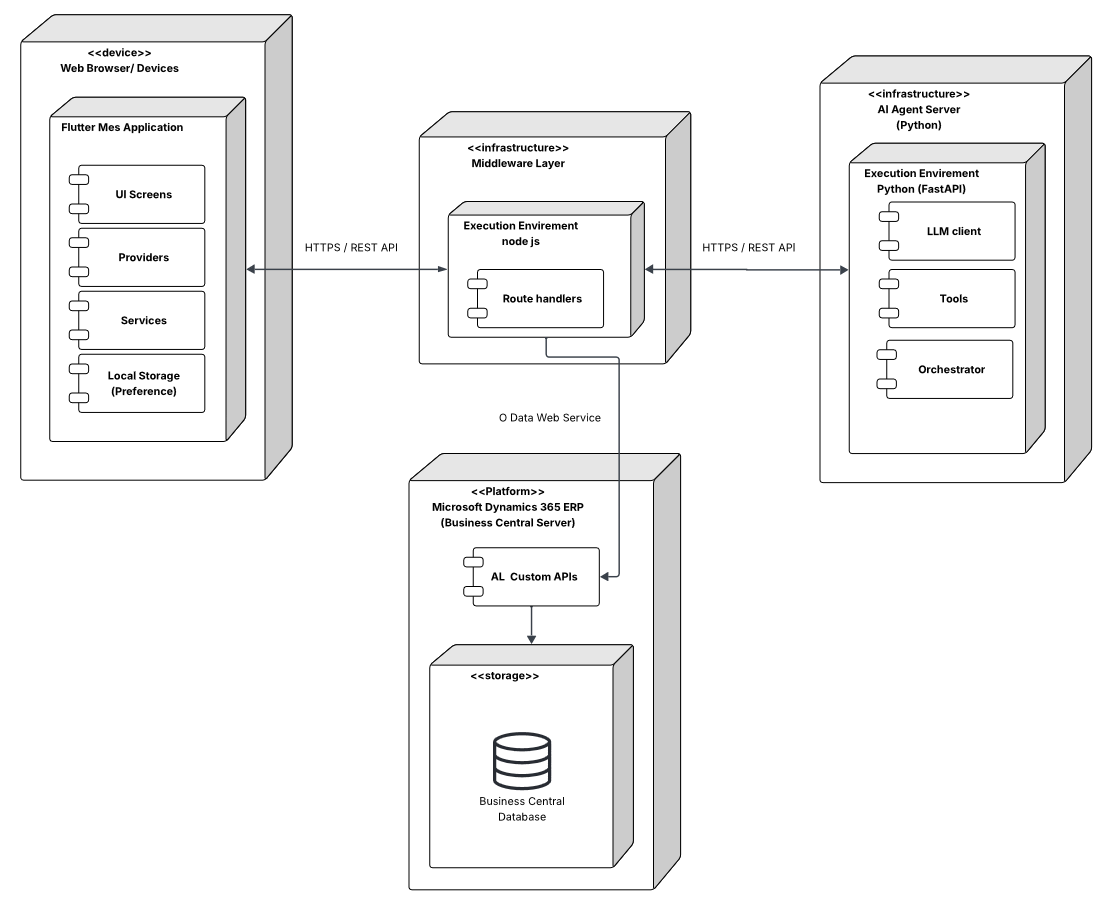
\includegraphics[width=\linewidth,keepaspectratio]{./media/MES_chapter-2-repport/systemArchitecture.png}
	\caption{MES System Physical Architecture}
	\label{fig:mescha-archi_physique}
\end{figure}

\subsection{Software Architecture}

The software architecture of the system is organised around four distinct layers.

\subsubsection{AL Back-end (Business Central)}

The back-end is structured in five layers:

\begin{itemize}
	\item \textbf{Tables (1-Tables)}: define the persistent data model; 
	MES User, MES Auth Token, MES Machine Status, MES Operation State, 
	MES Operation Scrap, MES Operation Execution, MES Operation Progression,
	MES Settings, MES Component Scan, and MES User Execution Interaction.
	\item \textbf{Enums (2-Enum)}: define the enumerated types; MES User 
	Role (Operator, Supervisor, Admin), MES Machine Status (Idle, Working), 
	MES Operation State (Running, Paused, Finished, Cancelled, Interrupted), 
	MES Token State (Revoked, Pending, Active).
	\item \textbf{Codeunits (3-CodeUnit)}: contain the business logic; 
	MES Auth Mgt (authentication, tokens), MES Password Mgt (SHA-256 hashing), 
	MES Machine Fetch (read operations), MES Machine Write (state orchestration),
	MES Machine Insert (table writes), MES Machine Validation (business rule guards),
	MES Authentification (user authentication), and the \domainterm{Mes Web Service}
	(wrappers exposed as web services).
	\item \textbf{API Pages (4-API)}: expose data for reading/writing via the BC REST 
	API; employees, work centres.
	\item \textbf{Pages (5-Pages)}: administration and debugging interfaces 
	in the BC client (lists, cards, API debug page, etc...).
\end{itemize}

\subsubsection{Node.js Middleware}

	The Node.js middleware is the network bridge between the Flutter client and
	Business Central. It handles SSPI/Windows authentication for BC OData V4
	requests, exposes a unified REST API to the Flutter application, and routes
	AI chat requests (\texttt{POST /api/ai/chat}) to the Python AI agent.

\subsubsection{Python AI Agent}

The Python AI agent (FastAPI) provides the conversational intelligence layer.
It classifies user intent, executes tool chains against Business Central via
the Node.js middleware, enriches results with data-analysis helpers, and
synthesises natural-language replies using a configurable multi-provider LLM client.


\subsubsection{Flutter Front-end}

The Flutter front-end follows a three-layer architecture:

\begin{itemize}
	\item \textbf{Data}: contains data models (models) and HTTP services (services) that
	      communicate with BC endpoints via the \texttt{http} library.
	\item \textbf{Domain}: contains the providers (Provider pattern) that expose the
	      application state to widgets --- AuthProvider, MesUserProvider,
	      MesMachinesProvider, MachineordersProvider, etc.
	\item \textbf{Presentation}: contains the pages and widgets of the user interface,
	      organised by functional domain (auth, admin, machine) with dedicated responsive
	      layouts (mobile, tablet, PC).
\end{itemize}

% ── 2.5 ─────────────────────────────────────────────────────────────────────
\section{Work Environment}

\subsection{Software Environment}

Table~\ref{tab:mescha-env_logiciel} summarises the main tools and technologies used in
this project.

\begin{longtable}{@{}>{\centering\arraybackslash}m{0.09\linewidth}>{\centering\arraybackslash}m{0.38\linewidth}>{\centering\arraybackslash}m{0.49\linewidth}@{}}
	\caption{MES project software environment}
	\label{tab:mescha-env_logiciel} \\
	\toprule
	\textbf{Logo}                                                                   & \textbf{Tool / Technology}              & \textbf{Role in the project} \\
	\midrule
	\endfirsthead

	\toprule
	\textbf{Logo}                                                                   & \textbf{Tool / Technology}              & \textbf{Role in the project} \\
	\midrule
	\endhead

	\multicolumn{3}{r}{\small Continued on next page} \\
	\endfoot

	\endlastfoot

	% IMAGE PLACEHOLDER - insert logos in the left column
	
\includegraphics[width=\linewidth]{./media/MES_chapter-2-repport/Microsoft-Business-Central-Logo.png}&
	Microsoft Dynamics 365 Business Central &
	ERP platform hosting the AL back-end and business data \\[6pt]
	\midrule
	
\includegraphics[width=\linewidth]{./media/MES_chapter-2-repport/AL-language-logo.png}&
	AL Language (Application Language)&
	Development of the BC extension (tables, codeunits, API pages) \\[6pt]
	\midrule
	
\includegraphics[width=\linewidth]{./media/MES_chapter-2-repport/flutter-dart-logo.png}&
	Flutter (Dart)&
	Development of the cross-platform mobile/web application \\[6pt]
	\midrule
	
\includegraphics[width=\linewidth]{./media/MES_chapter-2-repport/VSCode-logo.png}&
	Visual Studio Code&
	Primary development environment (AL and Flutter) \\[6pt]
	\midrule
	
\includegraphics[width=\linewidth]{./media/MES_chapter-2-repport/github-logo.png}&
	Git / GitHub&
	Version control and collaboration \\[6pt]
	\midrule
	
\includegraphics[width=\linewidth]{./media/MES_chapter-2-repport/postman-logo.png}&
	Postman&
	Testing and validation of OData V4 endpoints \\[6pt]
	\midrule
	
\includegraphics[width=\linewidth]{./media/MES_chapter-2-repport/python.png}&
	Python (FastAPI)&
	AI agent layer: intent classification, multi-provider LLM synthesis, fuzzy
	machine resolution, and analytics enrichment. \\[6pt]
	\midrule
	
\includegraphics[width=\linewidth]{./media/MES_chapter-2-repport/node.png}&
	Node.js (Express 5.x)&
	Reverse-proxy middleware: Windows SSPI authentication toward Business Central,
	unified REST API for Flutter and Python clients. \\[6pt]
	\midrule
	
\includegraphics[width=\linewidth]{./media/MES_chapter-2-repport/lucid-chart-logo.png}&
	lucid chart&
	UML and system architecture diagramming \\[6pt]
	\midrule
\end{longtable}

\subsection{Development Environment}

% TODO: describe the machines used, OS, tool versions
\textit{[To be completed: include workstation specifications (OS, RAM, CPU), tool versions
(Flutter SDK, Dart SDK, Business Central version, VS Code extensions), and any specific
configuration details such as Docker setup or BC on-premises instance parameters.]}

\phantomsection
\section*{Conclusion}
\addcontentsline{toc}{section}{Conclusion}

In this chapter, we analysed and specified the functional and non-functional
requirements of the MES system, identified the actors and their interactions, and
presented the overall architecture of the solution. We also described the work
environment and the adopted Scrum methodology. The following chapters detail the work
carried out sprint by sprint, presenting the conceptual aspects and the results
obtained at the end of each iteration.
% ============================================================
	
	
% ============================================================
%  BIBLIOGRAPHY
% ============================================================


% ---------------------------------------------------------------------------
% Sprint 1 Authentication \& User Management
% ---------------------------------------------------------------------------
\chapter{Sprint 1 Authentication \& User Management}
\graphicspath{{./media/MES_Sprint-1-Repport/}}
\minitoc
\newpage
\section*{Introduction}
\addcontentsline{toc}{section}{Introduction}
% -----------------------------------------------------------------------

This sprint focuses on delivering a complete authentication and user management
module for the \domainterm{MES} application. The primary goal is to develop a
secure authentication system covering \uilabel{login}, \uilabel{logout}, and
password management, alongside role-based page access control to ensure each
user can only reach features appropriate to their role.

In addition, the \userrole{Administrator} is given the ability to add new MES
users, generate secure passwords on their behalf, change a user's role and
work-centre assignment, and activate or deactivate accounts. By the end of this
sprint, a fully functional \uilabel{login} screen, \uilabel{change password}
flow, \uilabel{admin user management dashboard}, \uilabel{role management dialog},
and \uilabel{logout} functionality will all be in place.


% -----------------------------------------------------------------------
\section{Sprint Backlog}
% -----------------------------------------------------------------------

This sprint covers \textbf{Domain 1:} \textbf{\domainterm{Authentication \& User Management}}.


% ----------------------------------------------------------
%  US-1.1
% ----------------------------------------------------------
\begin{longtable}{@{} P{0.09\linewidth} P{0.34\linewidth} P{0.53\linewidth} @{}}
	\caption{Story Backlog}
	\label{tab:s1-Story-Backlog}\\
	\toprule
	\textbf{ID} & \textbf{User Story} & \textbf{Tasks} \\
	\midrule
	\endfirsthead
	\toprule
	\textbf{ID} & \textbf{User Story} & \textbf{Tasks} \\
	\midrule
	\endhead
	\multicolumn{3}{r}{\small Continued on next page} \\
	\endfoot
	\bottomrule
	\endlastfoot
	
	\textbf{US-1.1}
	& As an \userrole{Administrator}, I need to assign access to each user so
	that users only access features appropriate to their role.
	& \noindent\textit{Business Central (AL)}
	\begin{itemize}[noitemsep, topsep=0pt, partopsep=0pt, leftmargin=*]
		\item Implement the functions \texttt{AdminCreateUser()}, and \texttt{AdminSetActive()} in codeunit \techname{MES Unbound Actions}.
		\item Expose \texttt{AdminCreateUser()}, and \texttt{AdminSetActive()} through codeunit \techname{MES Web Service}.
		\item Create API page \techname{MES User Create API}.
	\end{itemize}
\\ & &
	\noindent\textit{Flutter}
	\begin{itemize}[noitemsep, topsep=0pt, partopsep=0pt, leftmargin=*]
		\item Update \techname{ApiService} to consume the new endpoints.
		\item Implement  \techname{MesUserService} to consume \texttt{fetchMesUsers()} and \texttt{createMesUser()} endpoints.
		\item Create provider \techname{MesUserProvider} to manage its state.
	\end{itemize}
\\ & &
	\begin{itemize}[noitemsep, topsep=0pt, partopsep=0pt, leftmargin=*]
		
		\item Create widget \techname{AddUserDialog}.
		\item Implement role-based navigation in \techname{\_AuthGate}.
	\end{itemize}\\
	\midrule
		\textbf{US-1.2}
	& As a User (\userrole{Operator} / \userrole{Supervisor} / \userrole{Administrator}),
	I need to log into the system with my credentials so that I can access
	features appropriate to my role.
	& \noindent\textit{Business Central (AL)}
	\begin{itemize}[noitemsep, topsep=0pt, partopsep=0pt, leftmargin=*]
		\item Create the tables \techname{MES USER} and \techname{MES AuthToken}.
		\item Create enum \techname{MES UserRole}.
		\item Implement functions \texttt{MakeSalt()}, \texttt{HashPassword()}, and \texttt{VerifyPassword()} in codeunit \techname{MES Password Mgt}.
		\item Implement functions \texttt{CreateUser()}, \texttt{SetPassword()}, \texttt{ValidateCredentials()}, \texttt{IssueNewToken()}, \texttt{ValidateToken()}, \texttt{TouchToken()}, \texttt{Logout()}, \texttt{ValidateChangePassword()}, \texttt{ValidateAdminToken()}, \texttt{SetActive()}, and \texttt{CleanupExpiredTokens()} in codeunit \techname{MESAuthMgt}.
		\item Implement functions \texttt{Login()}, \texttt{Logout()}, \texttt{Me()}, and \texttt{ChangePassword()} in codeunit \techname{MES Unbound Actions}.
		\item Expose \texttt{Login()}, \texttt{Logout()}, \texttt{Me()}, and \texttt{ChangePassword()} in codeunit \techname{MES Web Service}.
	\end{itemize}
\\ & &
	\noindent\textit{Flutter}
	\begin{itemize}[noitemsep, topsep=0pt, partopsep=0pt, leftmargin=*]
		\item Implement \techname{ApiService} to consume the new endpoints.
		\item Create provider \techname{AuthProvider} to manage its state.
		\item Implement authentication routing in \techname{\_AuthGate}.
		\item Create page \techname{LoginPage}.
		\item Create \techname{AppConstants}.
	\end{itemize}\\
	\midrule
	\textbf{US-1.3}
	& As an \userrole{Administrator}, I need to search users.
	& \noindent\textit{Flutter}
	\begin{itemize}[noitemsep, topsep=0pt, partopsep=0pt, leftmargin=*]
		\item Implement user search in \techname{AddUserPage}.
		\item Implement role filtering in \techname{AddUserPage}.
		\item Combine role and search filters in \techname{AddUserPage}.
	\end{itemize} \\
	\midrule
	\textbf{US-1.4}
	& As an \userrole{Administrator}, I need to see a list of all \techname{MES}
	users with their details so that I can manage accounts.
	& \noindent\textit{Business Central (AL)}
	\begin{itemize}[noitemsep, topsep=0pt, partopsep=0pt, leftmargin=*]
		\item Create the function \techname{fetchAllMESUsers} in codeunit \techname{MES Unbound Actions}.
		\item Expose \techname{fetchAllMESUsers} through codeunit \techname{MES Web Service}.
	\end{itemize}
\\ & &
	\noindent\textit{Flutter}
	\begin{itemize}[noitemsep, topsep=0pt, partopsep=0pt, leftmargin=*]
		\item Create model \techname{MesUser}.
		\item Implement \texttt{MesUserService} to consume the new end point.
		\item Implement \texttt{MesUserProvider} to manage its state and its streams.
		\item Implement user list display in \techname{AddUserPage}.
		\item Create the widgets \techname{GeneratePasswordDialog} and \techname{EmployeeAvatar}.
	\end{itemize} \\
	\midrule
	\textbf{US-1.5}
	& As an \userrole{Administrator}, I need to generate and assign a temporary
	password to a user so that they can log in for the first time.
	& \noindent\textit{Business Central (AL)}
	\begin{itemize}[noitemsep, topsep=0pt, partopsep=0pt, leftmargin=*]
		\item Implement function \texttt{AdminSetPassword()} in codeunit \techname{MES Unbound Actions}.
		\item Expose \texttt{AdminSetPassword()} through codeunit \techname{MES Web Service}.
	\end{itemize}
\\ & &
	\noindent\textit{Flutter}
	\begin{itemize}[noitemsep, topsep=0pt, partopsep=0pt, leftmargin=*]
		\item Create widget \techname{GeneratePasswordDialog}.
		\item Update \techname{ApiService} to consume \texttt{adminSetPassword()}.
		\item Update \techname{AuthProvider} to account for the new functions in the service.
	\end{itemize}\\
	\midrule
	\textbf{US-1.6}
	& As an \userrole{Administrator}, I need to change the role and work-centre
	assignment of an existing user so that access rights stay current.
	& \noindent\textit{Business Central (AL)}
	\begin{itemize}[noitemsep, topsep=0pt, partopsep=0pt, leftmargin=*]
		\item Implement function \texttt{AdminChangeUserRole()} in codeunit \techname{MES Unbound Actions}.
		\item Expose \texttt{AdminChangeUserRole()} through codeunit \techname{MES Web Service}.
	\end{itemize}
\\ & &
	\noindent\textit{Flutter}
	\begin{itemize}[noitemsep, topsep=0pt, partopsep=0pt, leftmargin=*]
		\item Update \techname{MesUserService} to consume \texttt{changeUserRole()}.
		\item Update \techname{MesUserProvider} to account \texttt{changeUserRole()}.
		\item Create widget \techname{ChangeRoleDialog}.
	\end{itemize}\\
	\midrule
	\textbf{US-1.7}
	& As an \userrole{Administrator}, I need to activate or deactivate a user
	account so that access can be revoked without deleting the account.
	& \noindent\textit{Flutter}
	\begin{itemize}[noitemsep, topsep=0pt, partopsep=0pt, leftmargin=*]
		\item Update  \techname{ApiService} to account for \texttt{toggleUserActiveStatus()}.
		\item Update  \techname{AuthProvider} to account for \texttt{toggleUserActiveStatus()}.
		\item Integrate activate and deactivate actions in \techname{AddUserPage}.
	\end{itemize}\\
\end{longtable}

% -----------------------------------------------------------------------
\section{Design}
\subsection{Use Case Diagram}

The UML Use Case Diagram (Figure~\ref{fig:s1-use-case-diagram}) shows the three
primary actors (\userrole{Operator}, \userrole{Supervisor},
\userrole{Administrator}) and their interactions with the \domainterm{MES}
authentication and user management system. In addition to the core login,
logout, change password, and user creation flows, the diagram includes the
\uilabel{Change Role / Work Centre} and \uilabel{Activate / Deactivate Account}
use cases available exclusively to the \userrole{Administrator}.

\begin{figure}[H]
	\centering
	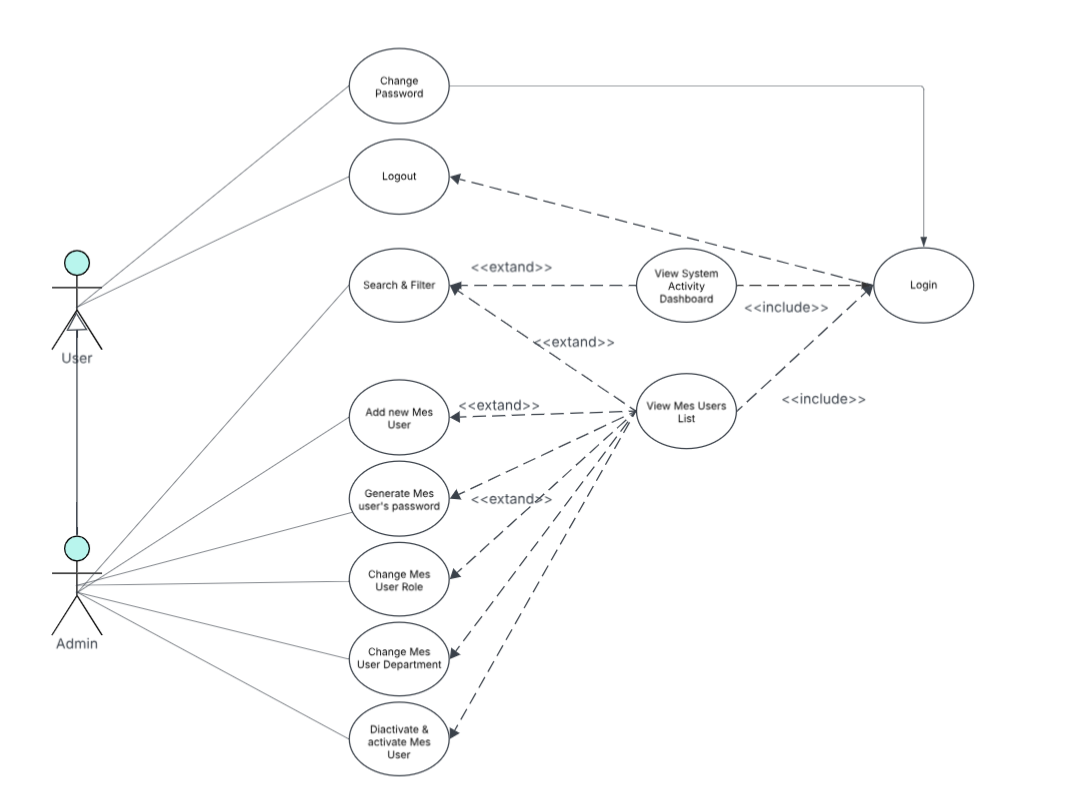
\includegraphics[width=\linewidth,keepaspectratio]{./media/MES_Sprint-1-Repport/diagrams/useCase/sprint1.png}
	\caption{UML Use Case Diagram.}
	\label{fig:s1-use-case-diagram}
\end{figure}

\Needspace{10\baselineskip}
\subsection{Textual Use Case Description}

\begin{longtable}{@{} P{0.22\linewidth} P{0.78\linewidth} @{}}
	
	\toprule
	\endfirsthead
	
	\midrule
	\endhead
	
	\multicolumn{2}{r}{\small Continued on next page}\\
	\endfoot
	
	\endlastfoot
	
	\textbf{Use Case Name}  & Login                                                                \\
	\midrule
	\textbf{Primary Actors} & \userrole{Operator}, \userrole{Supervisor}, \userrole{Administrator} \\
	\midrule
	\textbf{Preconditions}  &                                                                      
	\begin{itemize}[noitemsep, topsep=0pt, partopsep=0pt, leftmargin=*]
	\item The user account exists in the \techname{ERP} system.
	\item The user has an assigned role and department.
	\item The account must have a password (there is a possibility that
	there is an account without a password).
	\item The user account is active.
	\end{itemize} \\
	\midrule
	
	\textbf{Postconditions} &                                                                      
	\begin{itemize}[noitemsep, topsep=0pt, partopsep=0pt, leftmargin=*]
	\item If the credentials are valid, the user is successfully authenticated.
	\item A session token is generated and stored securely.
	\item The user is redirected to the appropriate dashboard based on their
	role (\userrole{Admin} or MES interface).
	\item If the \domainterm{need change password} flag is set to true, they
	are redirected to the \uilabel{Change Password} page.
	\item If the credentials are invalid, access is denied and an error
	message is displayed.
	\end{itemize} \\
	\midrule
	
	\textbf{Main Scenario}  &                                                                      
	\begin{enumerate}[noitemsep, topsep=0pt, partopsep=0pt, leftmargin=*]
	\item The user launches the application.
	\item The system displays the \uilabel{login screen}.
	\item The user enters \uilabel{Auth ID} and \uilabel{password}.
	\item The system automatically detects the device ID.
	\item The user clicks the \uilabel{Login} button.
	\item The system validates the credentials against the \techname{ERP} database.
	\item The system generates a secure session token.
	\item The system checks the user role.
	\item The system redirects the user to the appropriate dashboard
	(\userrole{Admin} or MES).
	\end{enumerate} \\
	\midrule
	\noalign{\vskip 4pt}
	\caption{Textual Use Case Description --- Login}
	\label{tab:s1-use-case-login}
	
\end{longtable}

\subsection{Sequence Diagrams}

The following sequence diagrams illustrate the communication flow between the
\techname{Flutter} frontend, the \techname{Business Central} OData layer, and
the \techname{AL} business logic for each authentication flow.
 
Figure~\ref{fig:s1-seq-login} depicts the login flow, in which the user submits
credentials, the \techname{AL} layer validates them against the
\techname{Business Central} user store, and the application either returns a
structured error or issues a session token and redirects the user to the
appropriate page based on their role and password-change flag.
\begin{figure}[H]
	\centering
	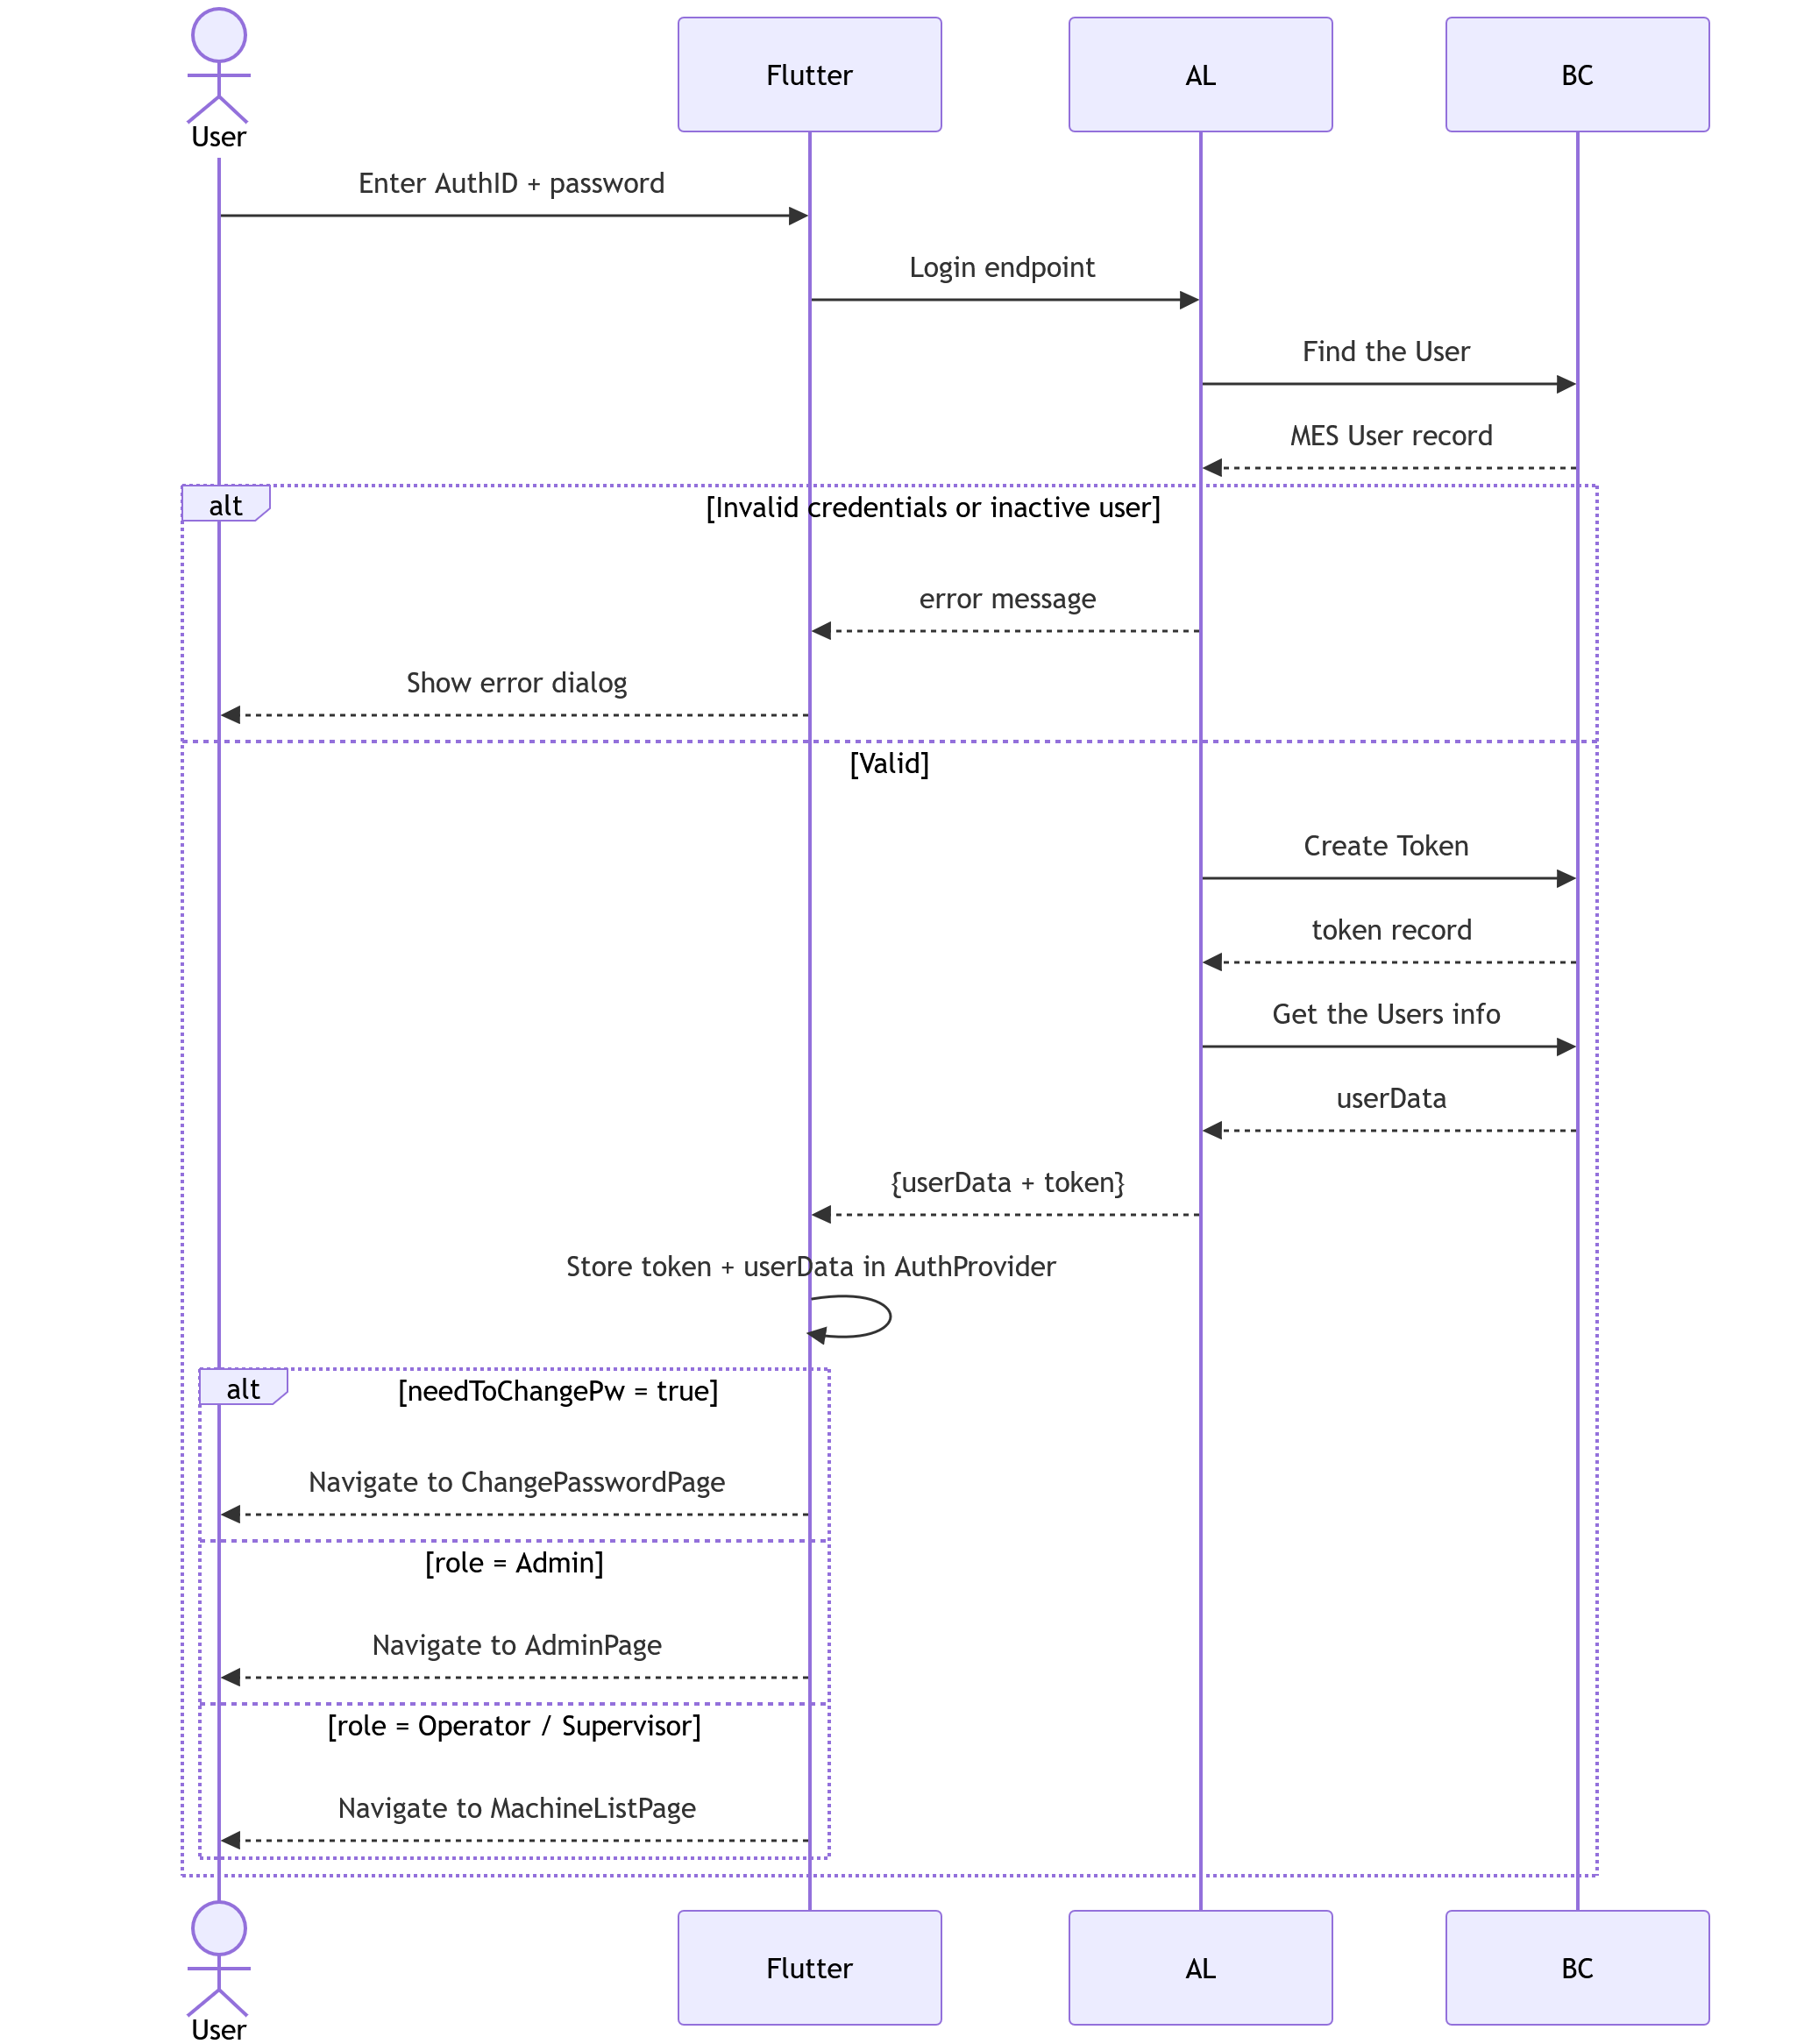
\includegraphics[width=\linewidth,height=0.82\textheight,keepaspectratio]{./media/MES_Sprint-1-Repport/diagrams/sequence/login.png}%
	\caption{SD-01: Login.}%
	\label{fig:s1-seq-login}%
\end{figure}%

%=====SD-01==========================================================
% sequenceDiagram
%    actor User
%    participant Flutter
%    participant AL
%    participant BC

%    User->>Flutter: Enter AuthID + password
%    Flutter->>AL: Login endpoint
%    AL->>BC: Find the User 
%    BC-->>AL: MES User record
%    alt Invalid credentials or inactive user
%        AL-->>Flutter: error message
%        Flutter-->>User: Show error dialog
%    else Valid
%        AL->>BC: Create Token
%        BC-->>AL: token record
%        AL->>BC: Get the Users info
%        BC-->>AL: userData
%        AL-->>Flutter: {userData + token}
%        Flutter->>Flutter: Store token + userData in AuthProvider
%        alt needToChangePw = true
%            Flutter-->>User: Navigate to ChangePasswordPage
%        else role = Admin
%            Flutter-->>User: Navigate to AdminPage
%        else role = Operator / Supervisor
%            Flutter-->>User: Navigate to MachineListPage
%        end
%    end
%====================================================================

Figure~\ref{fig:s1-seq-Token-Validation} presents the token validation flow,
which is invoked by the \techname{AL} backend before processing any
authenticated request. The backend retrieves the token record from
\techname{Business Central}, verifies its validity and expiry, confirms
that the associated user account is still active, and either updates the
\texttt{LastSeenAt} timestamp or returns an error that forces the
\techname{Flutter} client to redirect the user to the login page.
 

\begin{figure}[H]
	\centering
	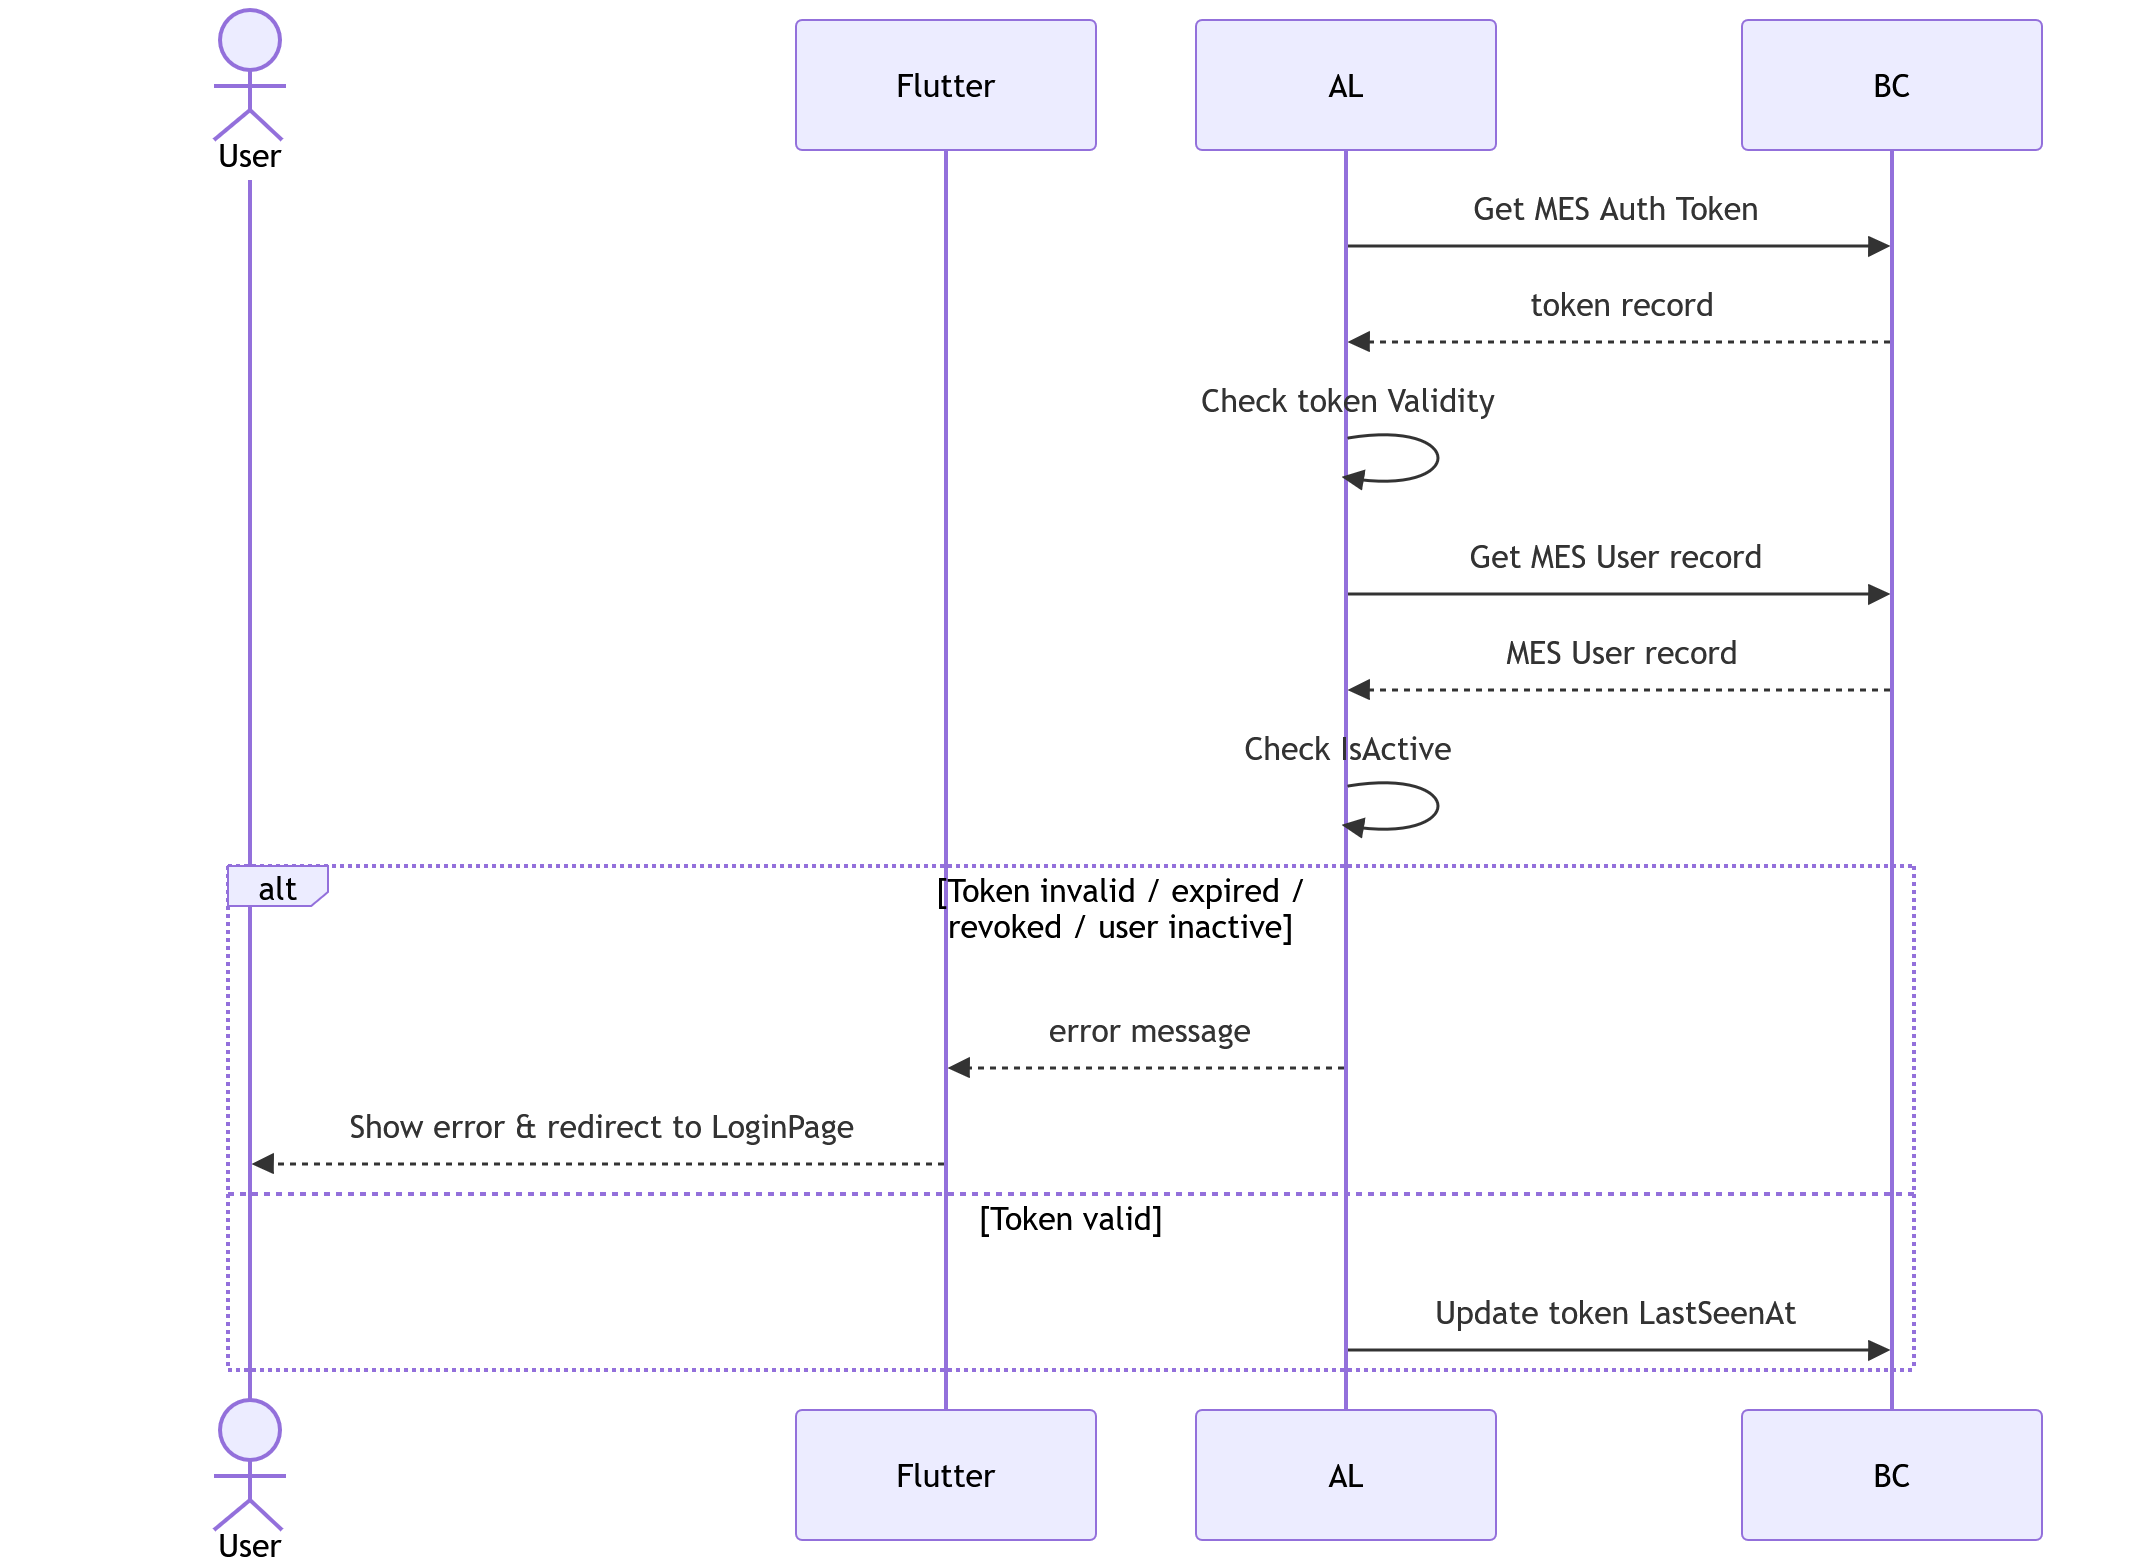
\includegraphics[width=\linewidth,height=0.82\textheight,keepaspectratio]{./media/MES_Sprint-1-Repport/diagrams/sequence/token-validation.png}%
	\caption{SD-02: Token Validation.}%
	\label{fig:s1-seq-Token-Validation}%
\end{figure}%

%======SD-02=========================================================
% sequenceDiagram
%     actor User
%     participant Flutter
%     participant AL
%     participant BC

%     AL->>BC: Get MES Auth Token
%     BC-->>AL: token record
%     AL->>AL: Check token Validity
%     AL->>BC: Get MES User record
%     BC-->>AL: MES User record
%     AL->>AL: Check IsActive
%     alt Token invalid / expired / revoked / user inactive
%         AL-->>Flutter: error message
%         Flutter-->>User: Show error & redirect to LoginPage
%     else Token valid
%         AL->>BC: Update token LastSeenAt
%     end
%====================================================================

Figure~\ref{fig:s1-seq-logout} illustrates the logout flow, in which the
\techname{Flutter} client sends a logout request, the \techname{AL} layer
retrieves and revokes the current session token in \techname{Business Central},
and the client clears its local \techname{AuthProvider} state before
navigating back to the login page.

\begin{figure}[H]
	\centering
	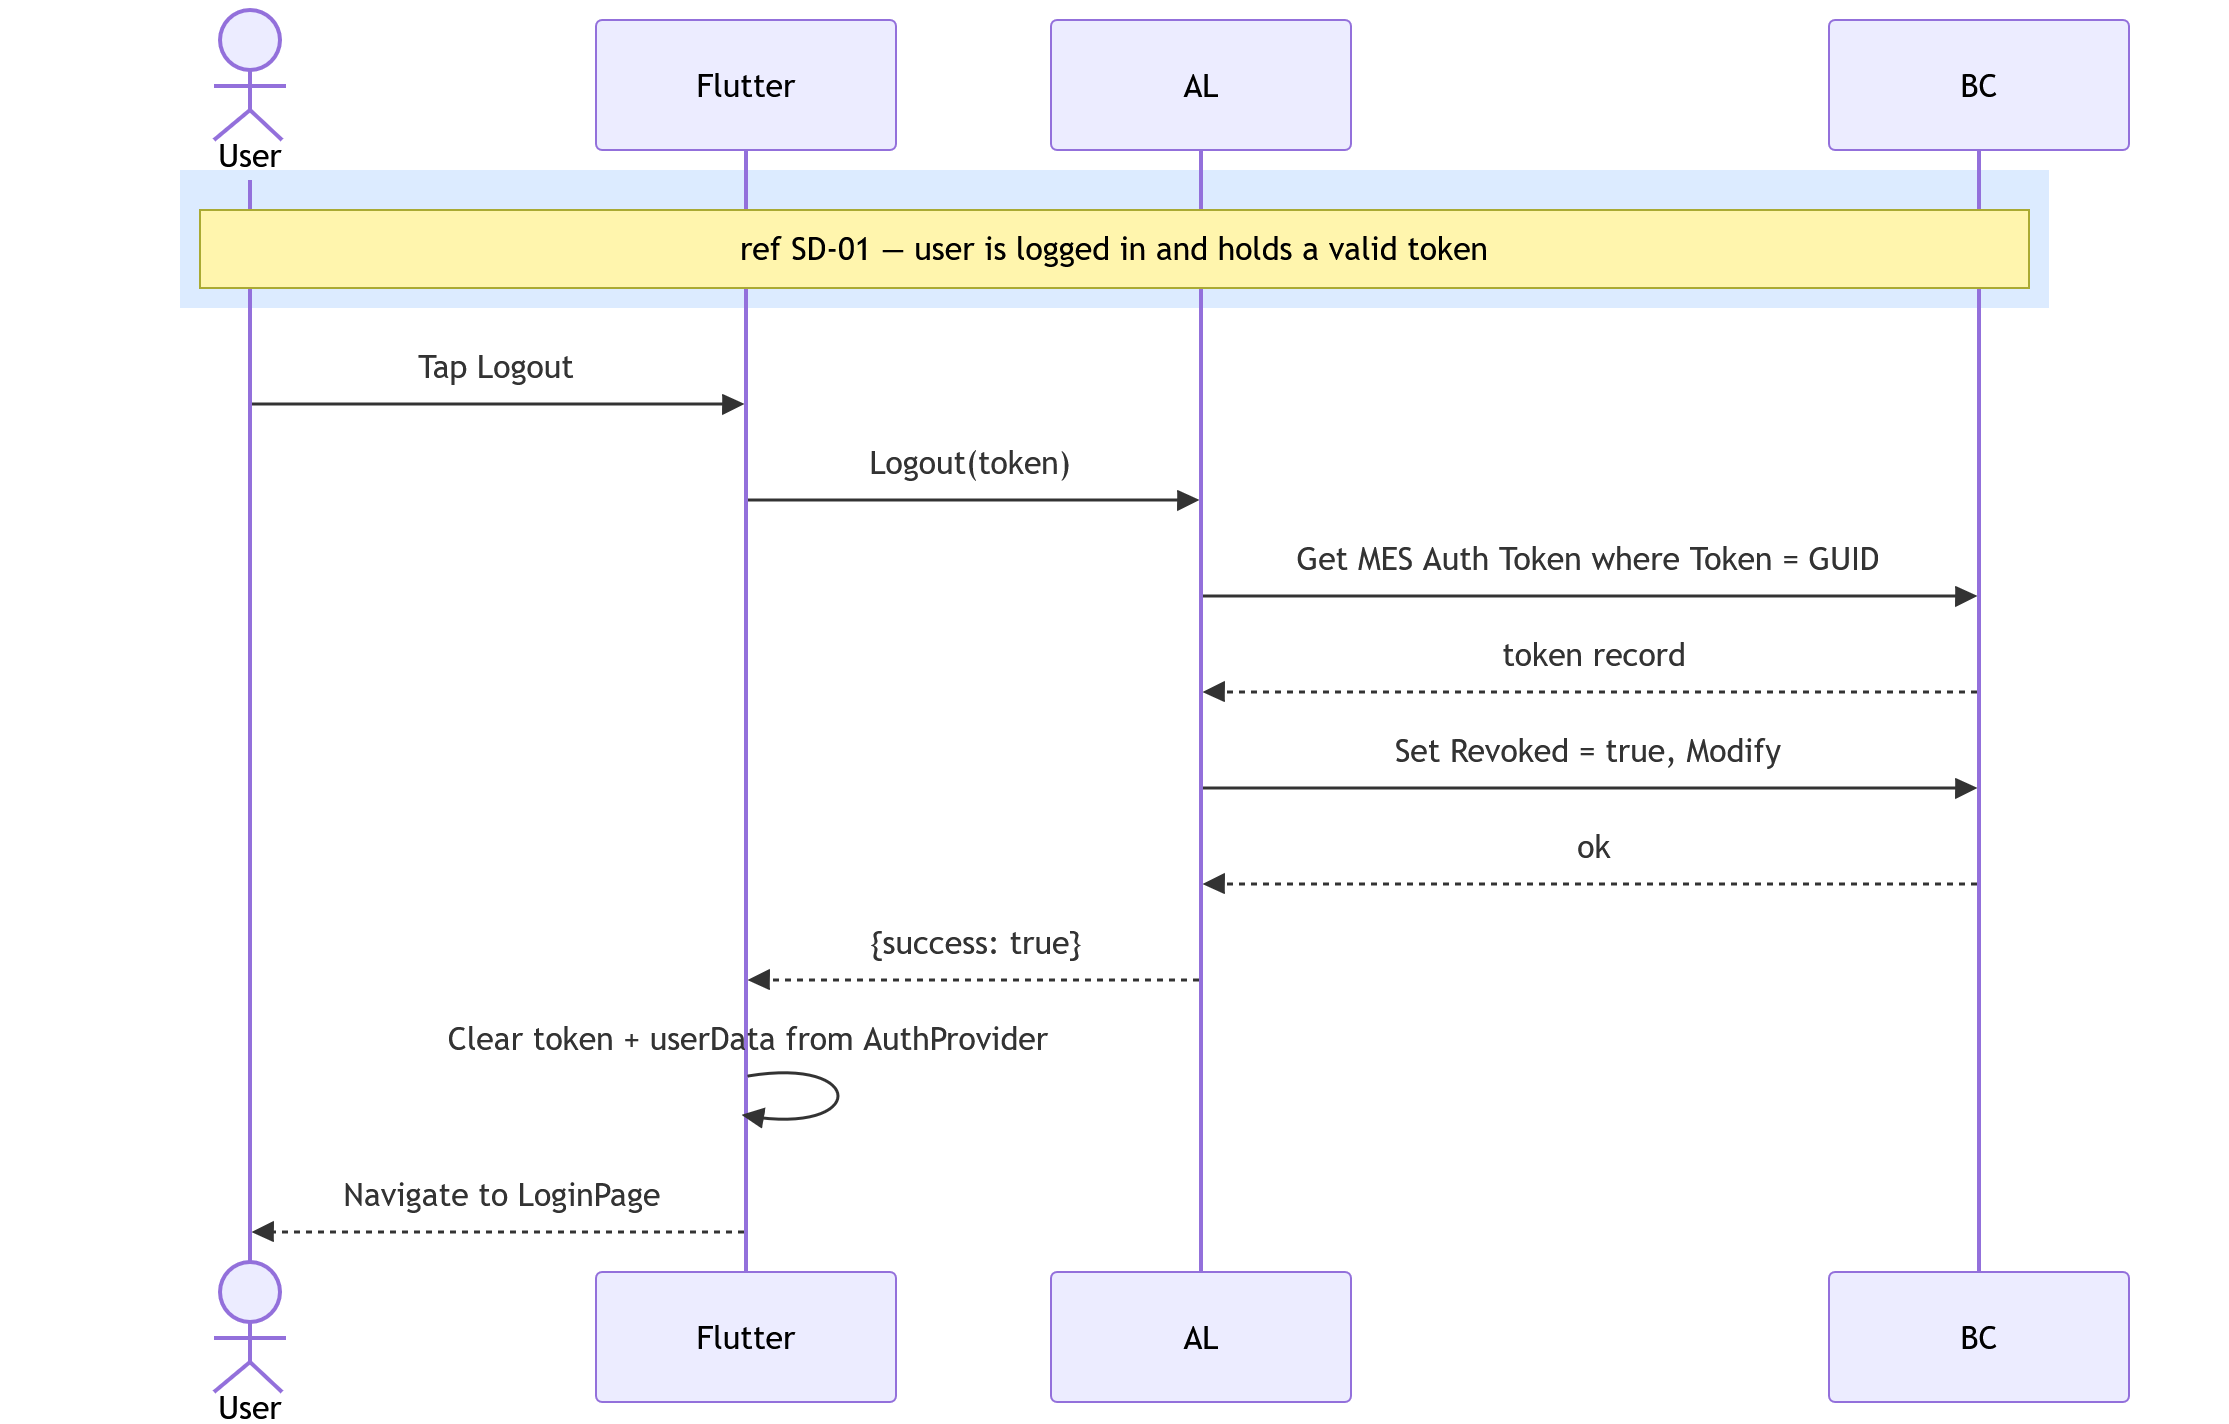
\includegraphics[width=\linewidth,height=0.82\textheight,keepaspectratio]{./media/MES_Sprint-1-Repport/diagrams/sequence/logout.png}%
	\caption{SD-03: Logout}%
	\label{fig:s1-seq-logout}%
\end{figure}%

%======SD-03=========================================================
% sequenceDiagram
%     actor User
%     participant Flutter
%     participant AL
%     participant BC

%     rect rgb(220,235,255)
%         Note over User,BC: ref SD-01 — user is logged in and holds a valid token
%     end

%     User->>Flutter: Tap Logout
%     Flutter->>AL: Logout request
%     AL->>BC: Get Token record
%     BC-->>AL: token record
%     AL->>BC: Revoke token
%     BC-->>AL: ok
%     AL-->>Flutter: success message
%     Flutter->>Flutter: Clear token + userData from AuthProvider
%     Flutter-->>User: Navigate to LoginPage
%====================================================================

Figure~\ref{fig:s1-seq-ChangePw} describes the change-password flow. The
\techname{Flutter} client first validates locally that the two password
fields match and satisfy the strength rules, then forwards the request to
the \techname{AL} layer, which re-validates the token (SD-02), verifies
the current password hash, checks the new password strength, and — on
success — updates the credential record in \techname{Business Central}
and revokes all existing tokens for the account.

\begin{figure}[H]
	\centering
	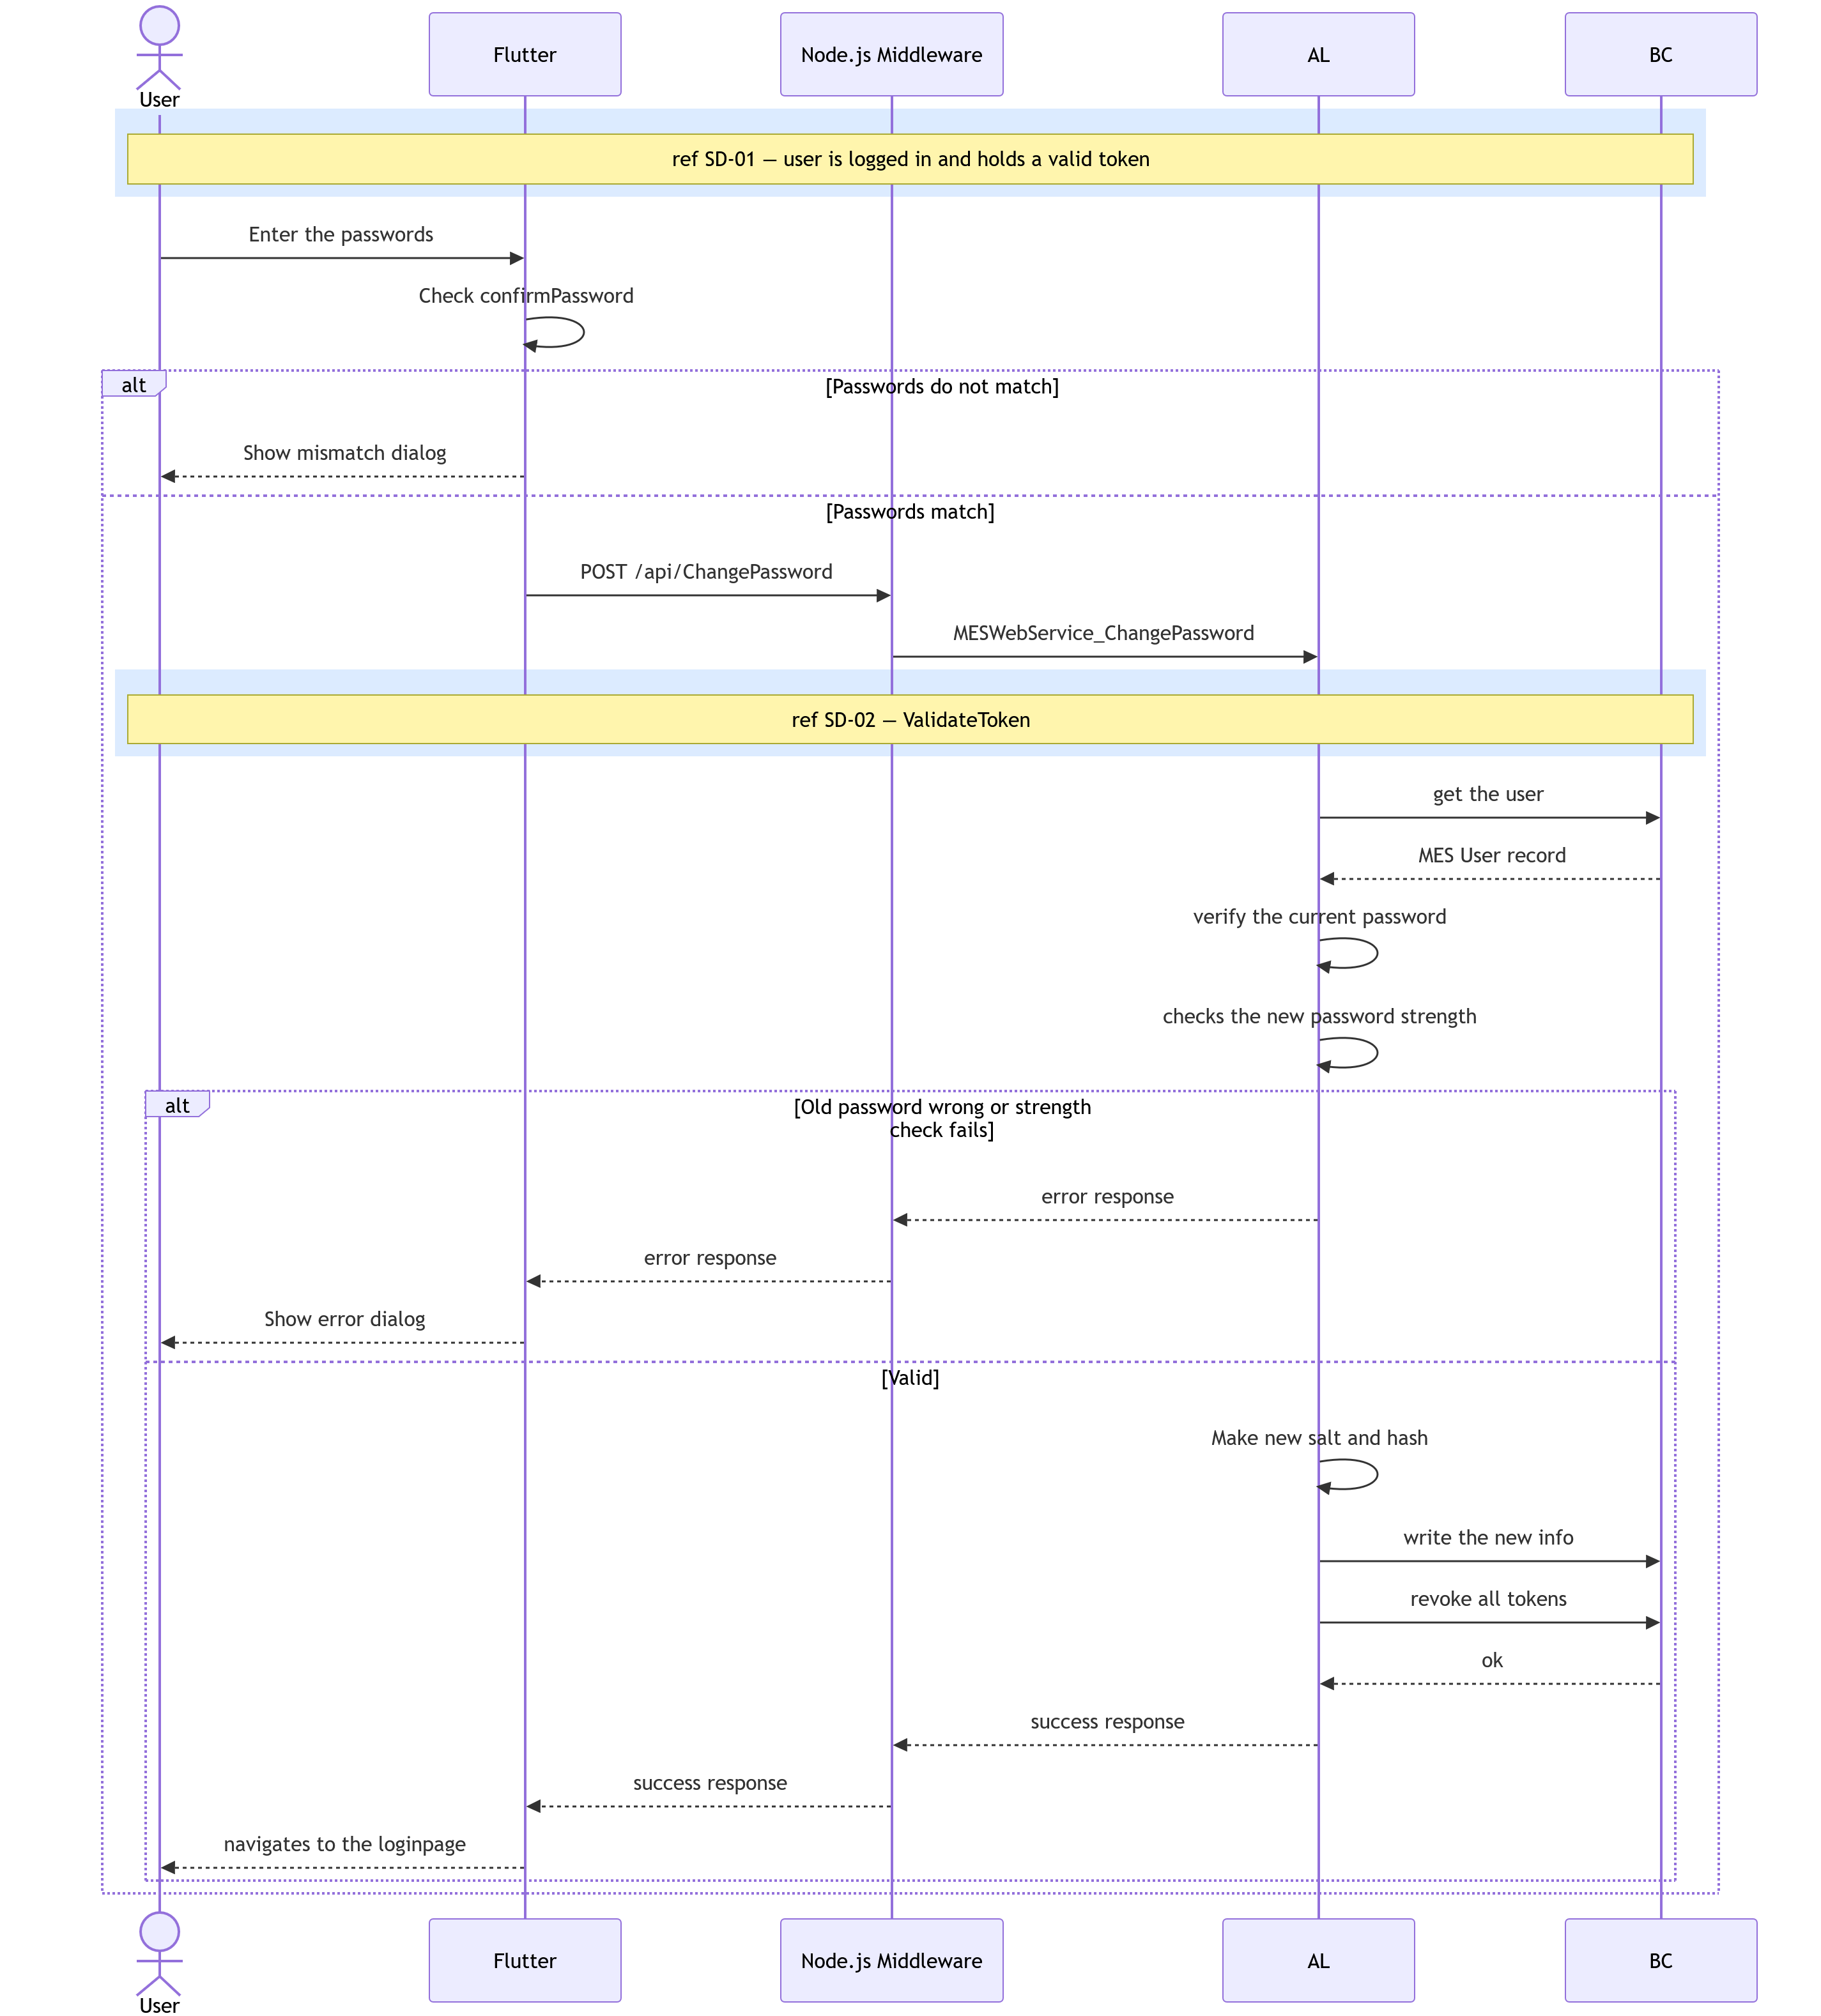
\includegraphics[width=\linewidth,height=0.82\textheight,keepaspectratio]{./media/MES_Sprint-1-Repport/diagrams/sequence/change-password.png}%
	\caption{SD-03: Change Password}%
	\label{fig:s1-seq-ChangePw}%
\end{figure}%


%======SD-04=========================================================
% sequenceDiagram
%     actor User
%     participant Flutter
%     participant AL
%     participant BC

%     rect rgb(220,235,255)
%         Note over User,BC: ref SD-01 — user is logged in and holds a valid token
%     end

%     User->>Flutter: Enter current password + new password
%     Flutter->>Flutter: Validate passwords match and meet strength rules
%     Flutter->>AL: ChangePassword request

%     rect rgb(220,235,255)
%         Note over User,BC: ref SD-02 — AL validates token before proceeding
%     end

%     AL->>BC: Get MES User (from token)
%     BC-->>AL: MES User record (storedHash, salt)
%     AL->>AL: check old password
%     AL->>AL: IsPasswordStrong(newPw)
%     alt Validation failed
%         AL-->>Flutter: error message
%         Flutter-->>User: Show error dialog
%     else Valid
%         AL->>BC: Update MES User with new password
%         AL->>BC: Revoke all tokens of the user
%         BC-->>AL: ok
%         AL-->>Flutter: success message
%         Flutter->>Flutter: Update AuthProvider 
%         Flutter-->>User: Navigate to AdminPage / MachineListPage
%     end
%====================================================================

Figures~\ref{fig:s1-seq-AdminCreateUser} through~\ref{fig:s1-seq-AdminToggleActive}
cover the four administrator user-management operations. All four follow the
same pattern: the \techname{Flutter} client sends an admin-scoped request,
the \techname{AL} layer validates the token and confirms that the caller
holds the \userrole{Admin} role (SD-02), executes the requested
\techname{Business Central} write operations, and triggers a reactive refresh
so that the updated user list is reflected immediately in the UI.
 
Figure~\ref{fig:s1-seq-AdminCreateUser} shows the user creation flow, in which
the \techname{AL} layer inserts a new \domainterm{MES User} record with
\texttt{IsActive} and \texttt{NeedToChangePw} set to \texttt{true}, then
iterates over the supplied work-centre list to create the corresponding
assignment records.

\begin{figure}[H]
	\centering
	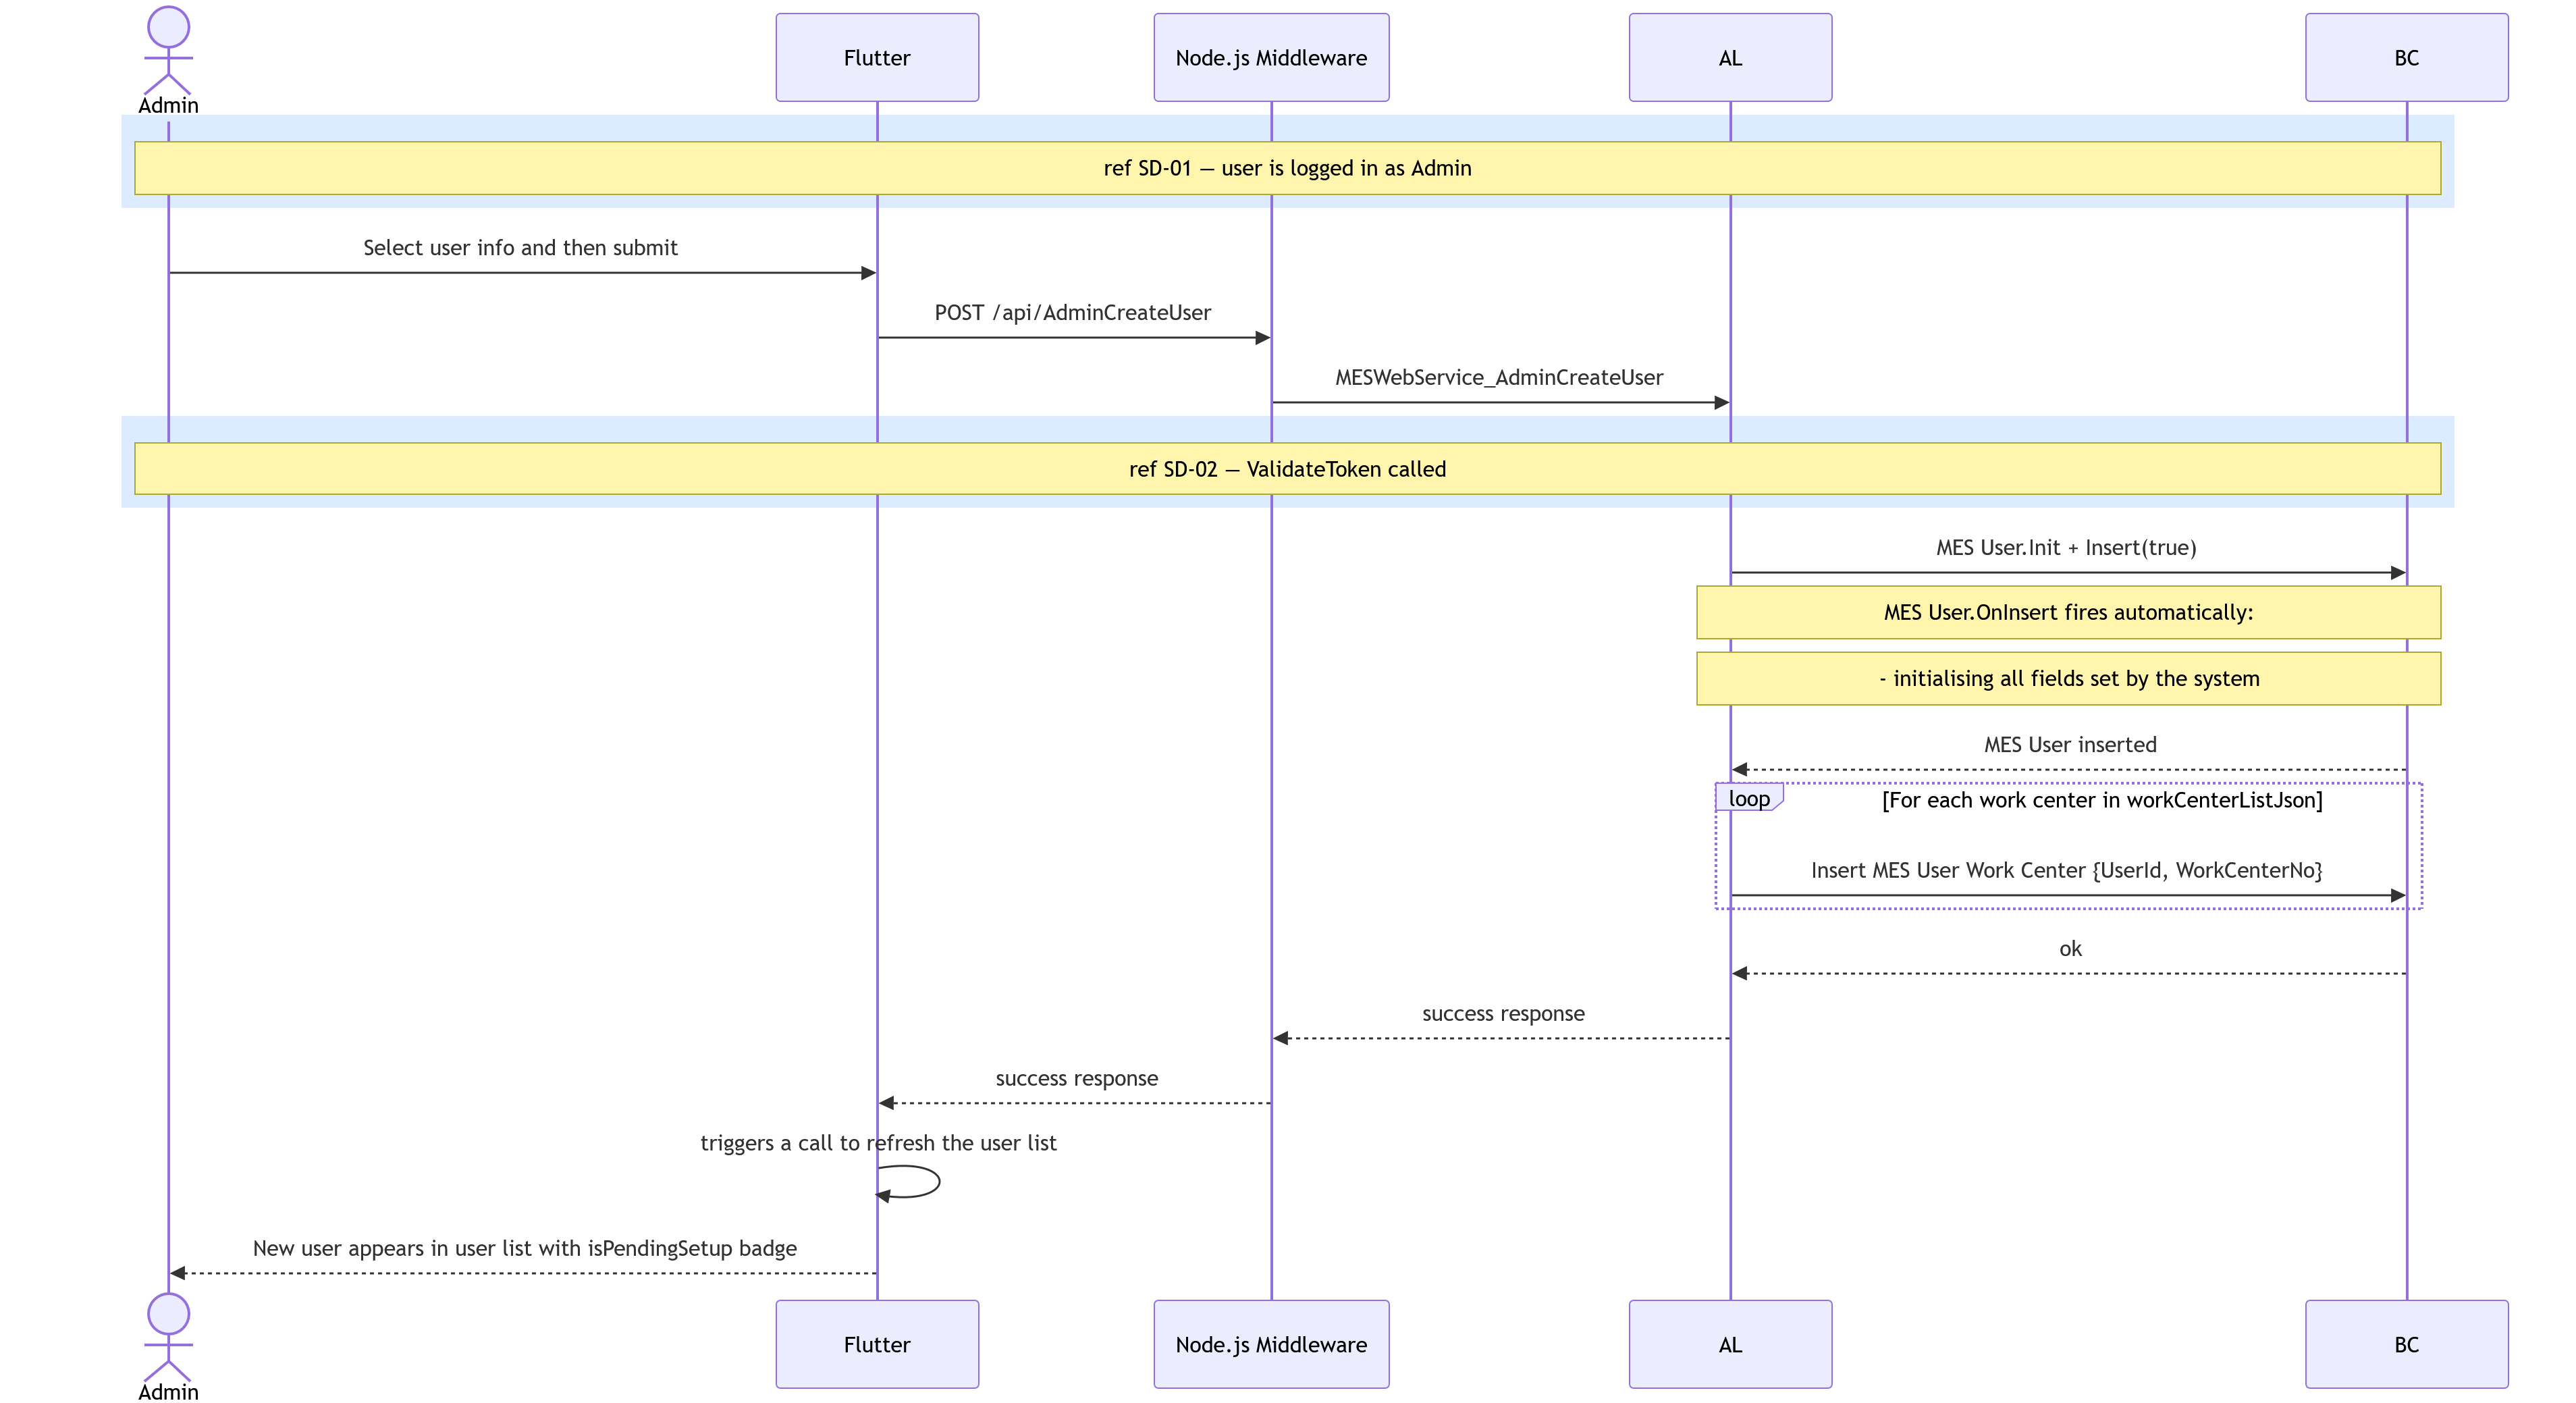
\includegraphics[width=\linewidth,height=0.82\textheight,keepaspectratio]{./media/MES_Sprint-1-Repport/diagrams/sequence/admin-create-user.png}%
	\caption{SD-05: Admin - Create User.}%
	\label{fig:s1-seq-AdminCreateUser}%
\end{figure}%

%=====SD:05==========================================================
% sequenceDiagram
%     actor User
%     participant Flutter
%     participant AL
%     participant BC

%     rect rgb(220,235,255)
%         Note over User,BC: ref SD-01 — user is logged in as Admin
%     end

%     User->>Flutter: Add a User
%     Flutter->>AL: AdminCreateUser request

%     rect rgb(220,235,255)
%         Note over User,BC: ref SD-02 — AL validates token and checks Role = Admin
%     end

%     AL->>BC: Insert MES User with IsActive and NeedToChangePw as true
%     BC-->>AL: ok
%     loop For each work center in workCenterListJson
%         AL->>BC: Insert MES User Work Center
%     end
%     BC-->>AL: ok
%     AL-->>Flutter: success message
%     Flutter->>Flutter: triggerRefresh — MES user stream re-emits
%     Flutter-->>User: New user appears in user list
%====================================================================

Figure~\ref{fig:s1-seq-AdminSetPw} depicts the admin set-password flow. The
administrator generates a temporary credential, the \techname{AL} layer marks
the target account as requiring a password change on next login, revokes all
active tokens for that account, and returns the new credential to the
\techname{Flutter} client as copyable text.

\begin{figure}[H]
	\centering
	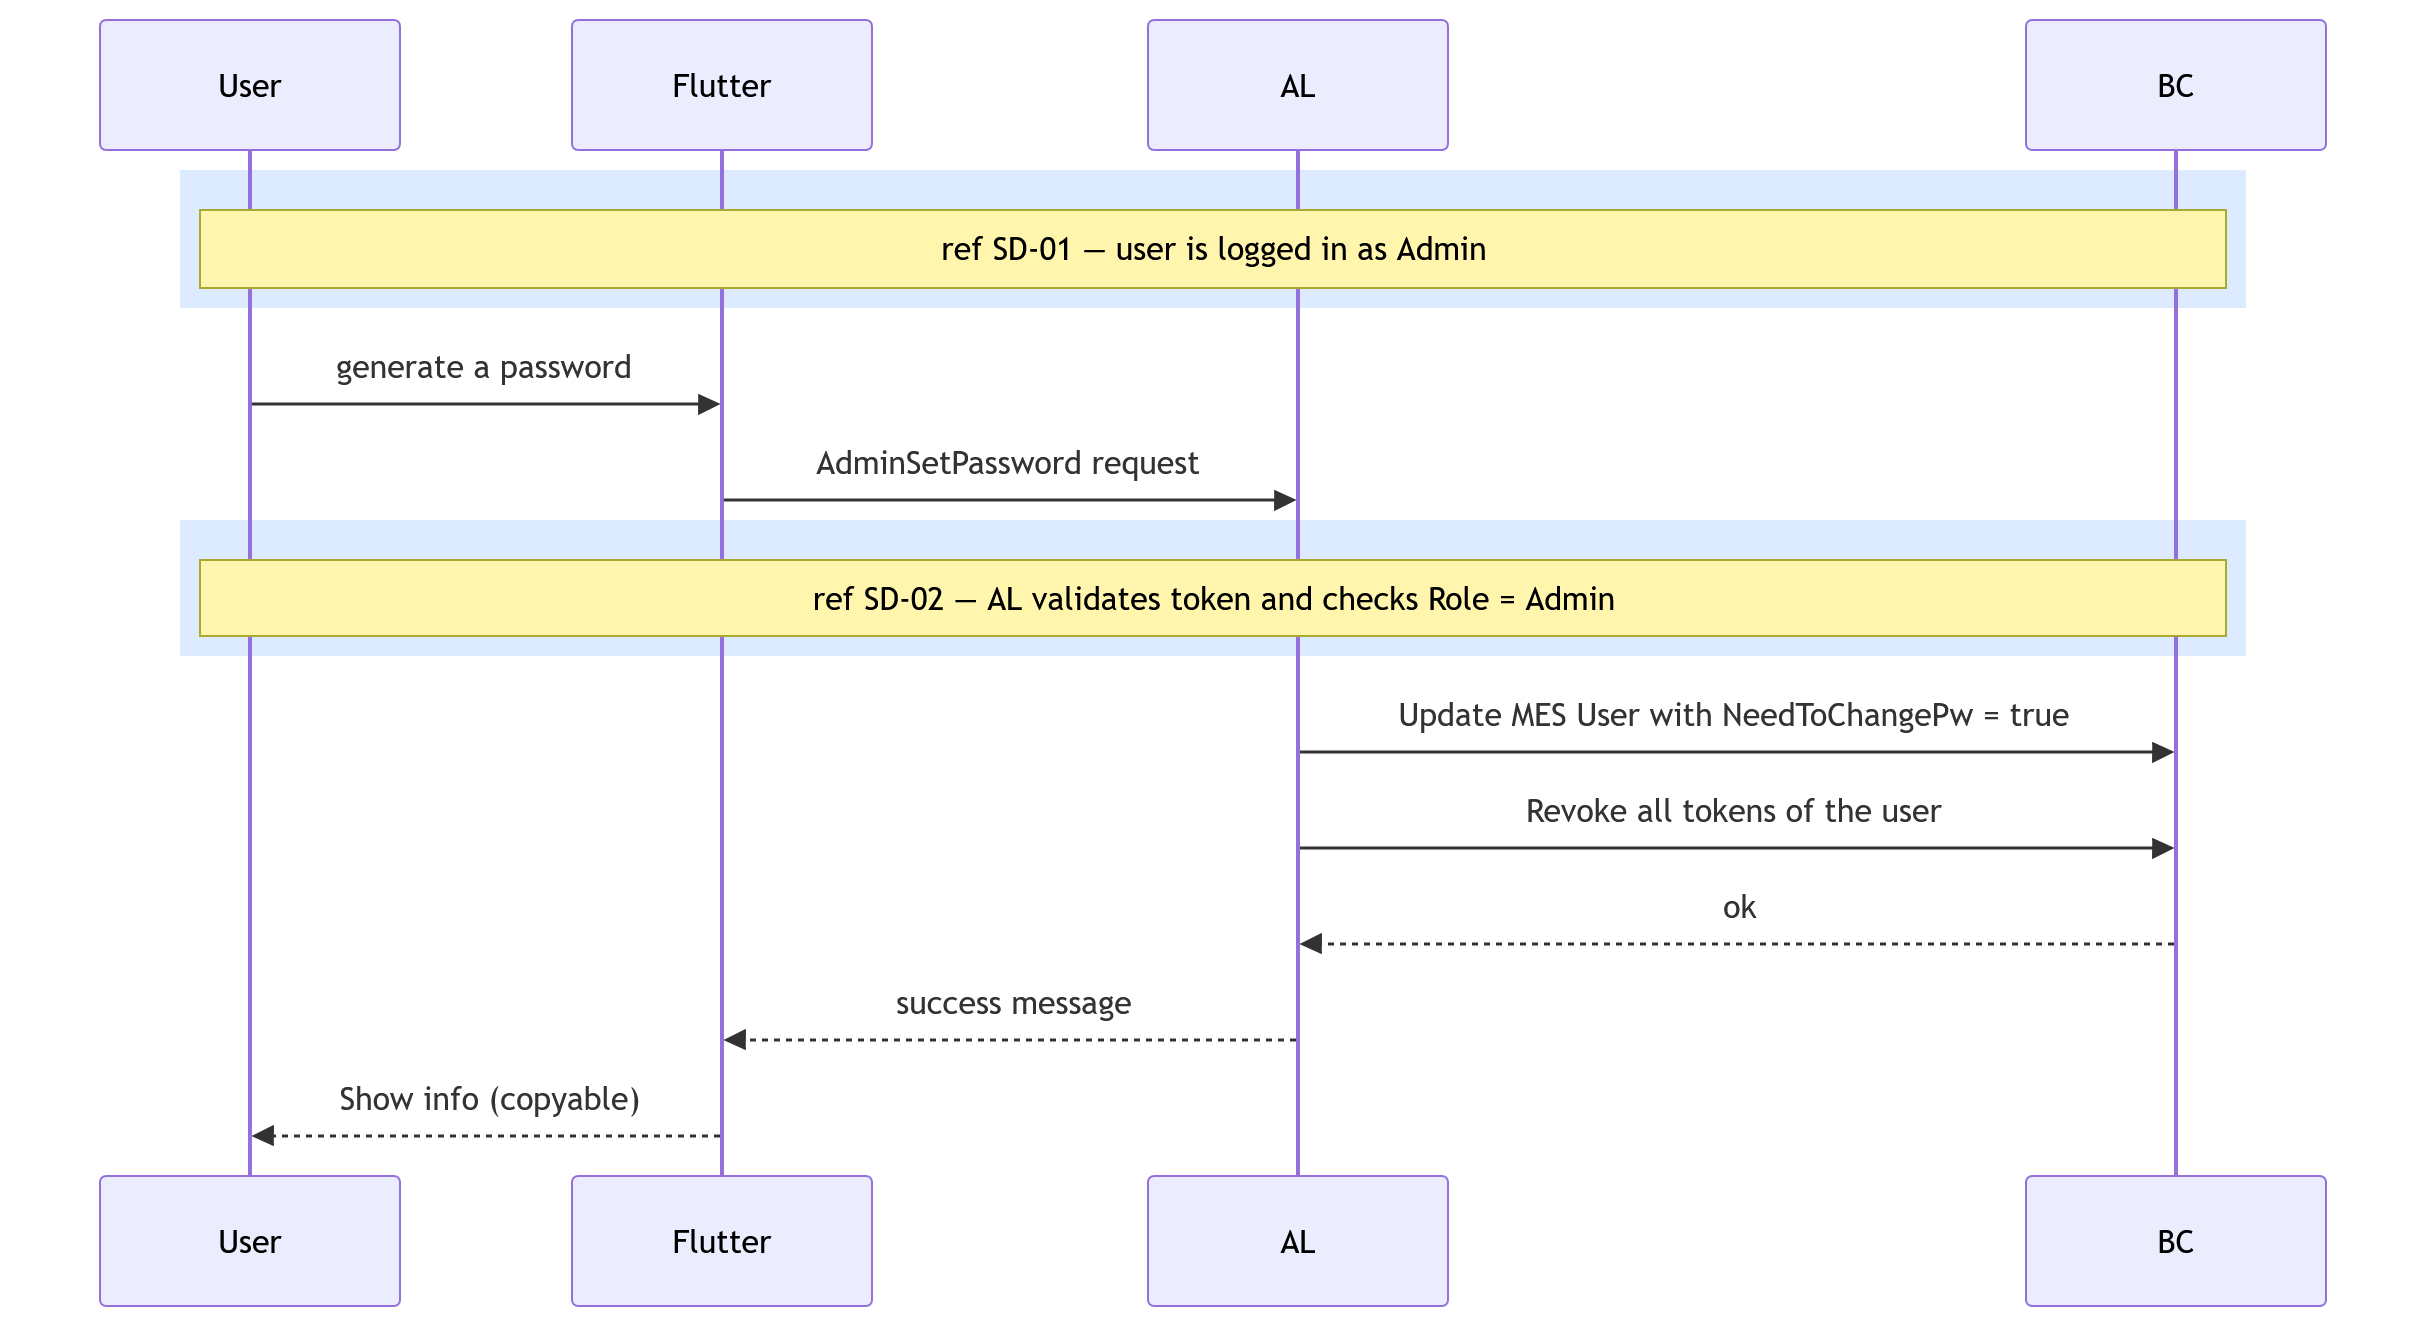
\includegraphics[width=\linewidth,height=0.82\textheight,keepaspectratio]{./media/MES_Sprint-1-Repport/diagrams/sequence/admin-set-password.png}%
	\caption{SD-06: Admin - Set Password.}%
	\label{fig:s1-seq-AdminSetPw}%
\end{figure}%


%=====SD-06==========================================================
% sequenceDiagram
%     actor User
%     participant Flutter
%     participant AL
%     participant BC

%     rect rgb(220,235,255)
%         Note over User,BC: ref SD-01 — user is logged in as Admin
%     end

%     User->>Flutter: generate a password
%     Flutter->>AL: AdminSetPassword request

%     rect rgb(220,235,255)
%         Note over User,BC: ref SD-02 — AL validates token and checks Role = Admin
%     end

%     AL->>BC: Update MES User with  NeedToChangePw = true
%     AL->>BC: Revoke all tokens of the user
%     BC-->>AL: ok
%     AL-->>Flutter: success message
%     Flutter-->>User: Show info (copyable)
%====================================================================

Figure~\ref{fig:s1-seq-AdminSetPw} depicts the admin set-password flow. The
administrator generates a temporary credential, the \techname{AL} layer marks
the target account as requiring a password change on next login, revokes all
active tokens for that account, and returns the new credential to the
\techname{Flutter} client as copyable text.

\begin{figure}[H]
	\centering
	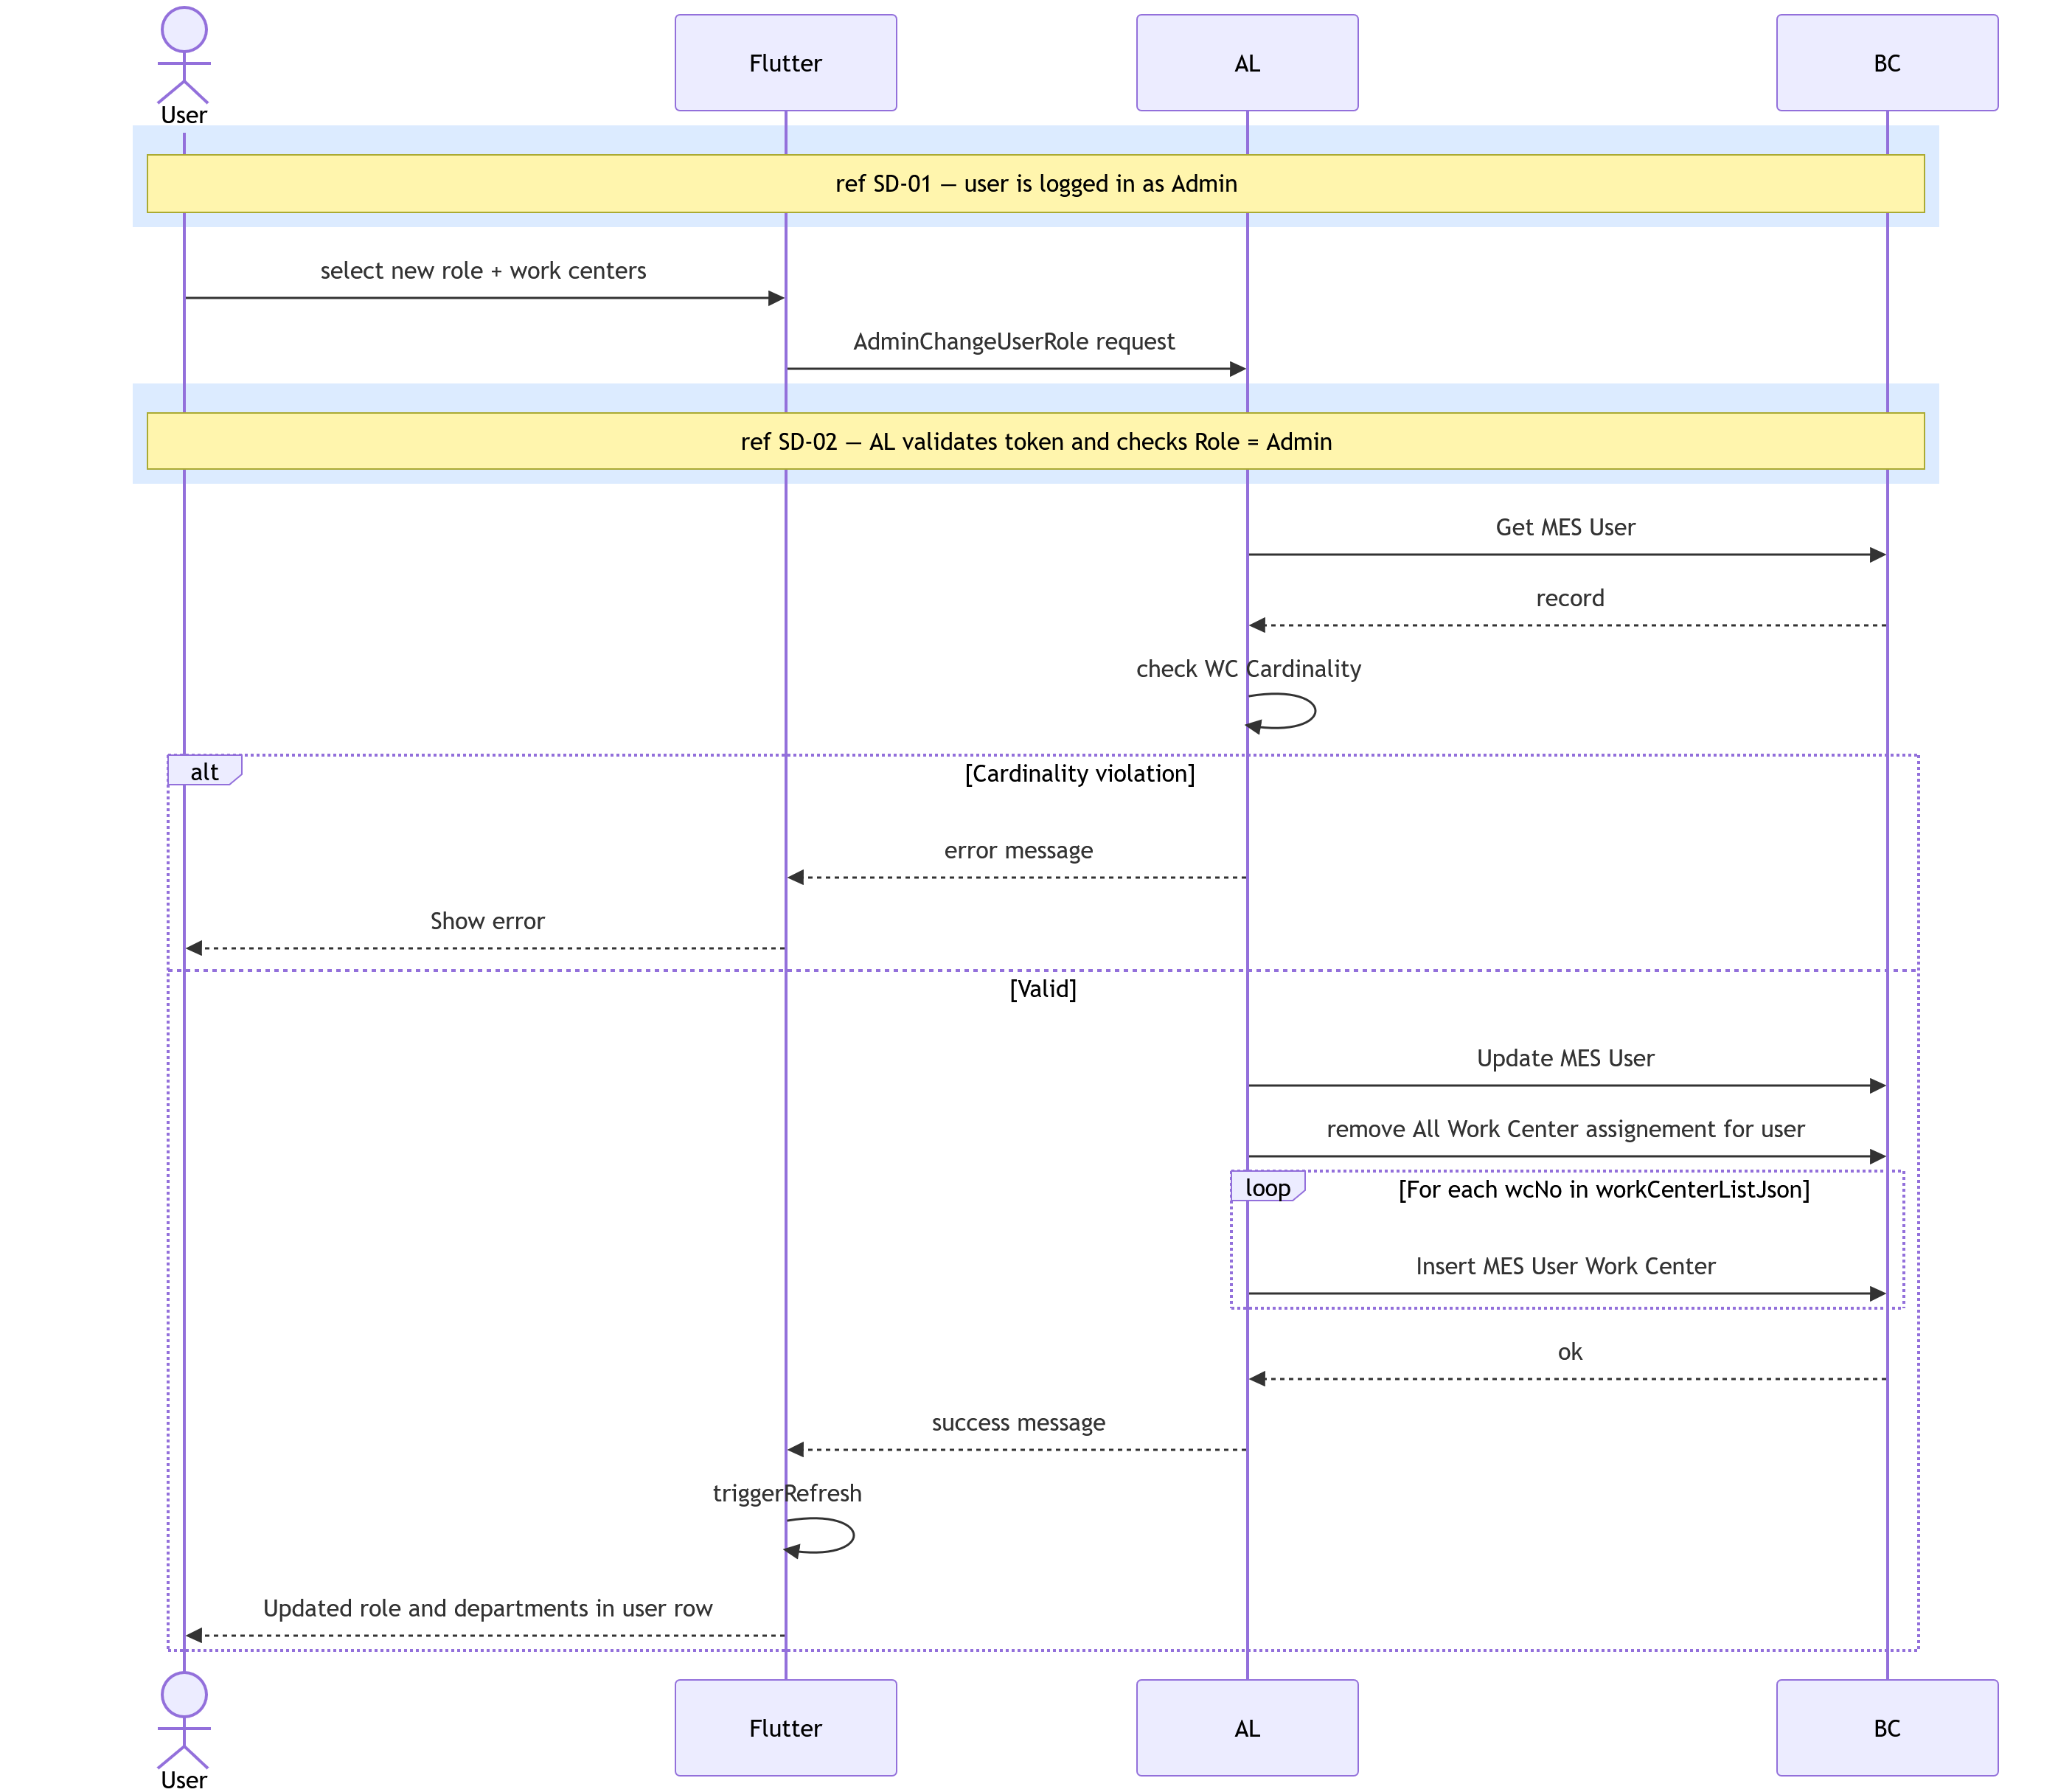
\includegraphics[width=\linewidth,height=0.82\textheight,keepaspectratio]{./media/MES_Sprint-1-Repport/diagrams/sequence/admin-change-role_departement.png}%
	\caption{SD-07: Admin - Change Role / Work Centre.}%
	\label{fig:s1-seq-AdminChangeRole}%
\end{figure}%

%=====SD-07===============================================================
% sequenceDiagram
%     actor User
%     participant Flutter
%     participant AL
%     participant BC

%     rect rgb(220,235,255)
%         Note over User,BC: ref SD-01 — user is logged in as Admin
%     end

%     User->>Flutter: select new role + work centers
%     Flutter->>AL: AdminChangeUserRole request

%     rect rgb(220,235,255)
%         Note over User,BC: ref SD-02 — AL validates token and checks Role = Admin
%     end

%     AL->>BC: Get MES User
%     BC-->>AL: record
%     AL->>AL: check WC Cardinality
%     alt Cardinality violation
%         AL-->>Flutter: error message
%         Flutter-->>User: Show error
%     else Valid
%         AL->>BC: Update MES User
%         AL->>BC: remove All Work Center assignement for user
%         loop For each wcNo in workCenterListJson
%             AL->>BC: Insert MES User Work Center
%         end
%         BC-->>AL: ok
%         AL-->>Flutter: success message
%         Flutter->>Flutter: triggerRefresh
%         Flutter-->>User: Updated role and departments in user row
%     end
%====================================================================

Figure~\ref{fig:s1-seq-AdminToggleActive} presents the account activation and
deactivation flow. When deactivating an account, the \techname{AL} layer
additionally revokes all active session tokens for that user, ensuring that
any currently authenticated sessions are immediately invalidated.

\begin{figure}[H]
	\centering
	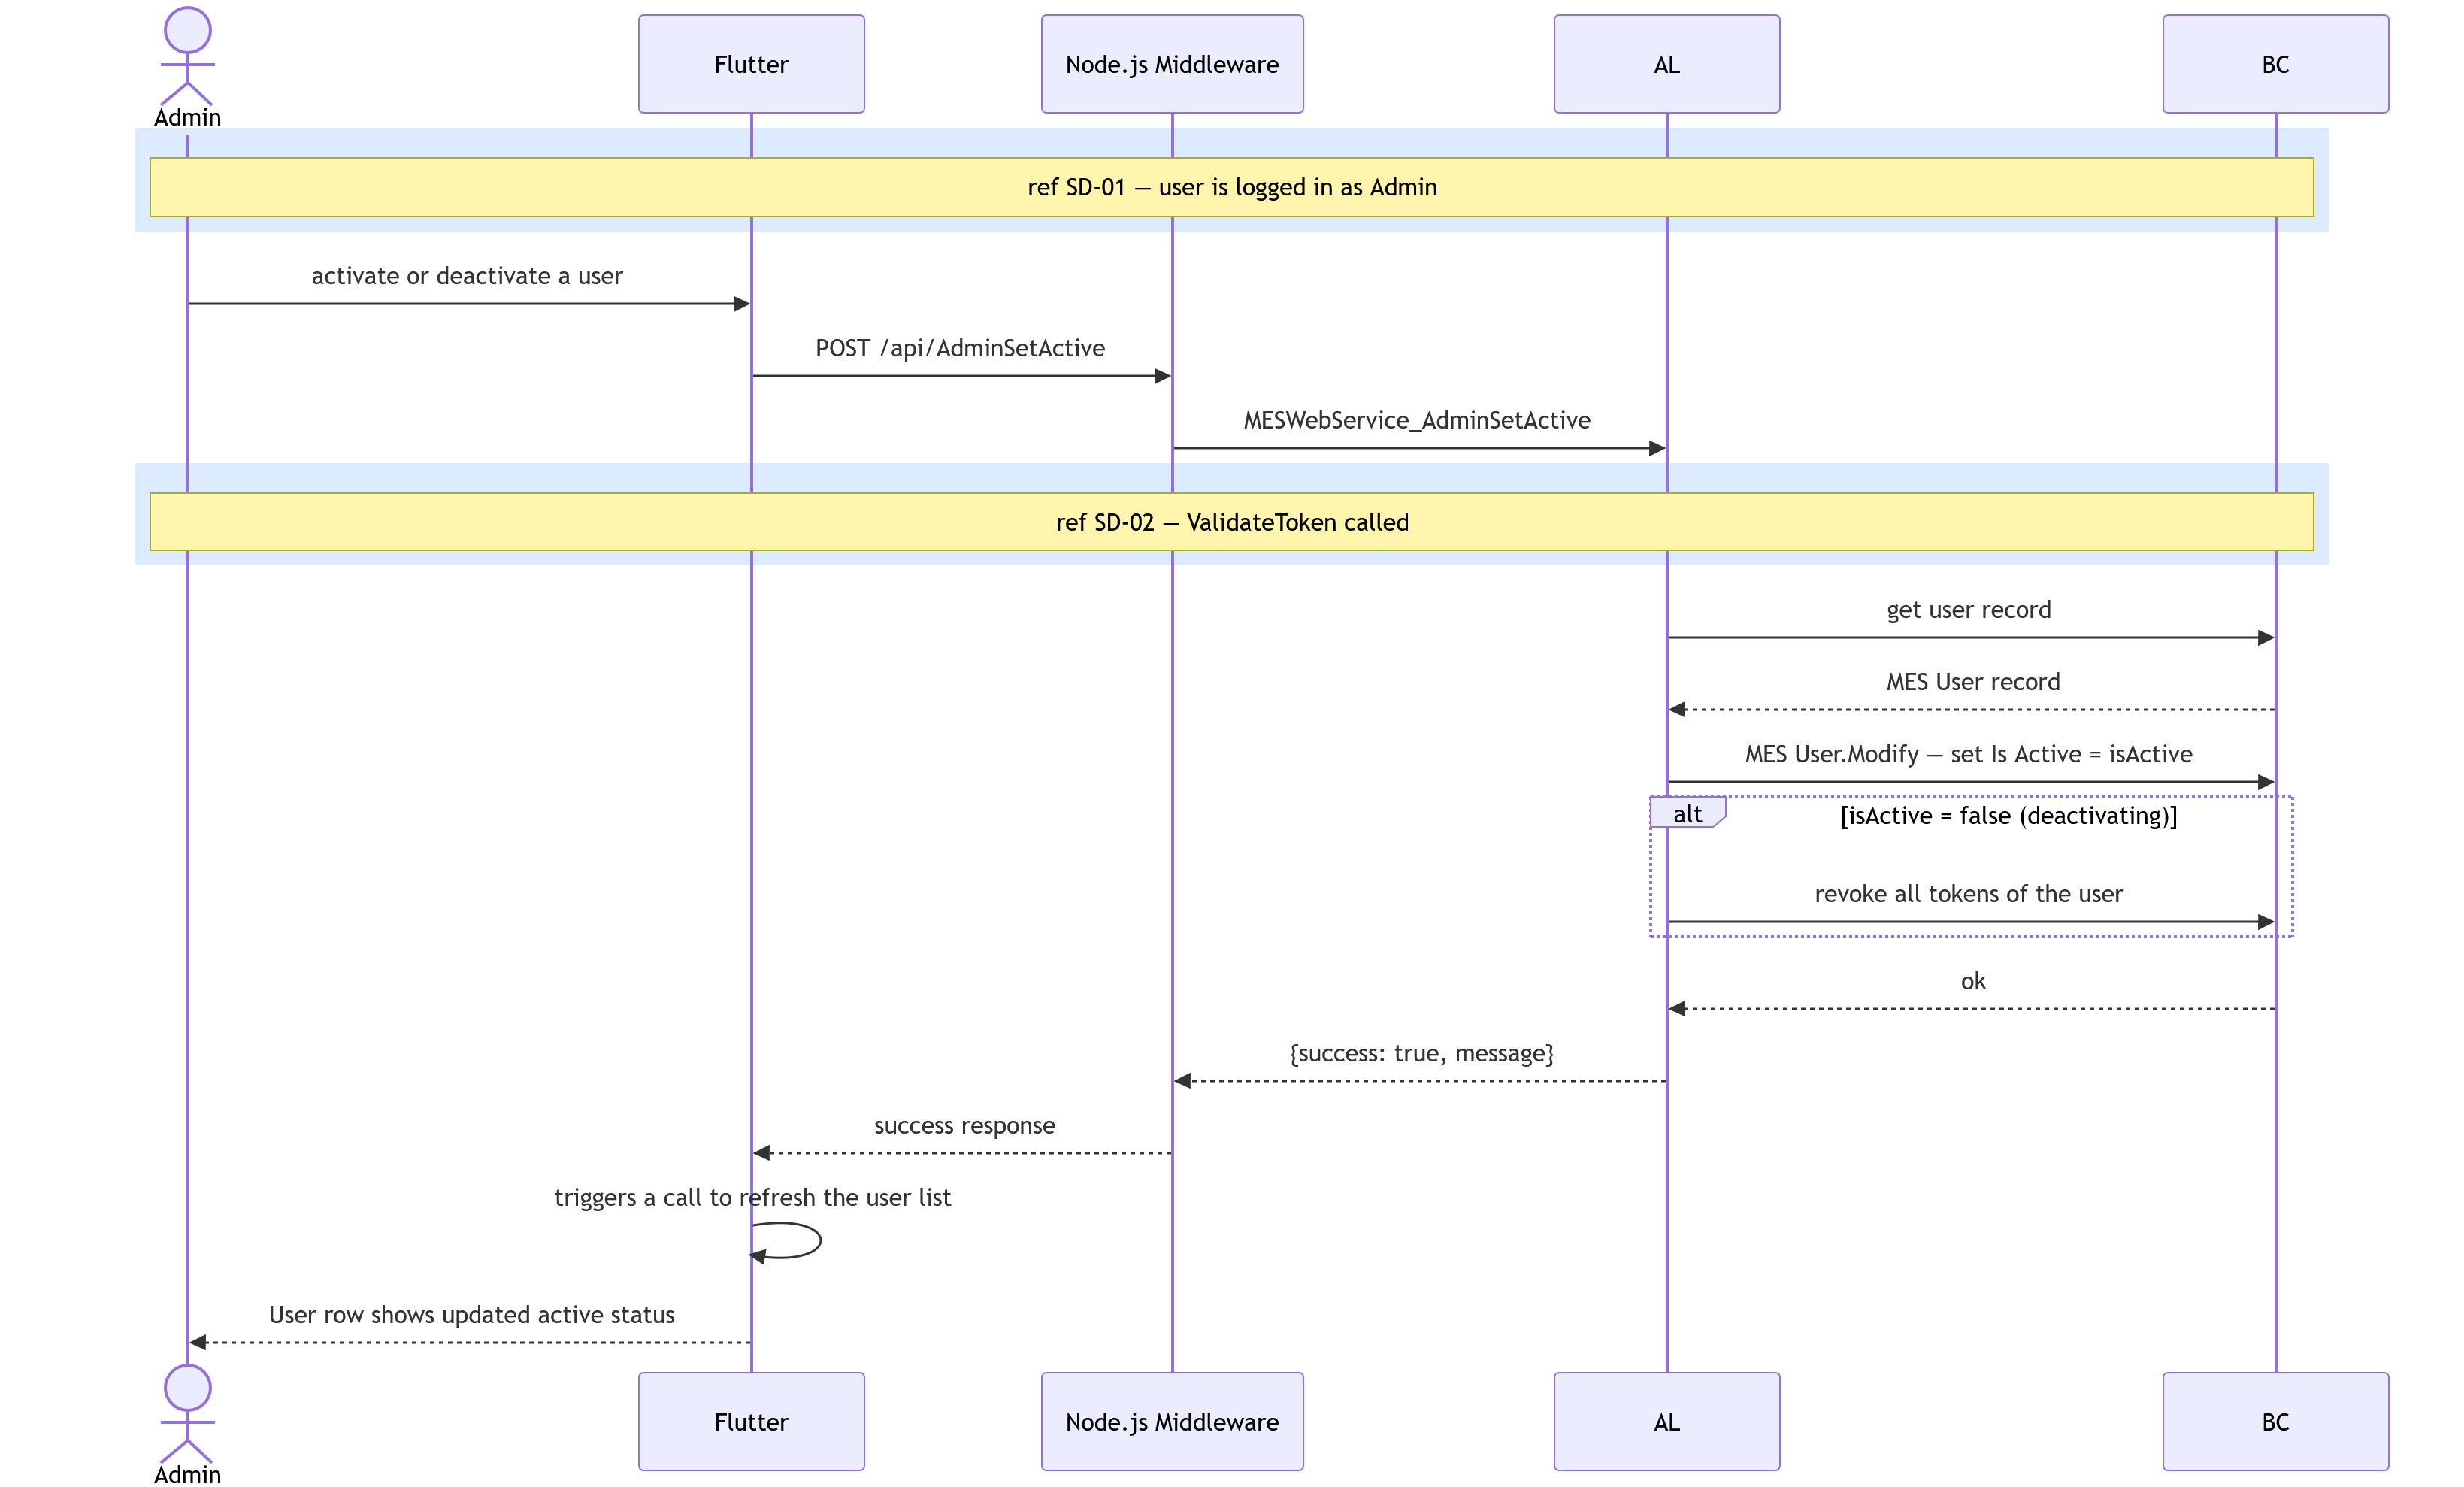
\includegraphics[width=\linewidth,height=0.82\textheight,keepaspectratio]{./media/MES_Sprint-1-Repport/diagrams/sequence/admin-toggle-account-active-status.png}%
	\caption{SD-08: Admin - Toggle Account Active Status.}%
	\label{fig:s1-seq-AdminToggleActive}%
\end{figure}%

%=====SD-08==========================================================
% sequenceDiagram
%     actor User
%     participant Flutter
%     participant AL
%     participant BC

%     rect rgb(220,235,255)
%         Note over User,BC: ref SD-01 — user is logged in as Admin
%     end

%     User->>Flutter: Activate or Deactivate user
%     Flutter->>AL: AdminSetActive request

%     rect rgb(220,235,255)
%         Note over User,BC: ref SD-02 — AL validates token and checks Role = Admin
%     end

%     AL->>BC: Get MES User
%     BC-->>AL: record
%     AL->>BC: Set IsActive
%     alt Deactivating
%         AL->>BC: Revok all tokens of the User
%     end
%     BC-->>AL: ok
%     AL-->>Flutter: success message
%     Flutter->>Flutter: triggerRefresh
%     Flutter-->>User: User row shows updated status
%====================================================================


\subsection{Class Diagram}

The UML Class Diagram of the \domainterm{MES} authentication domain, shown in
Figure~\ref{fig:s1-class-diagram}, depicts the \modulename{MesUser},
\modulename{AuthToken}, and \modulename{PasswordPolicy} classes with their
attributes and associations.

\begin{figure}[H]
	\centering
	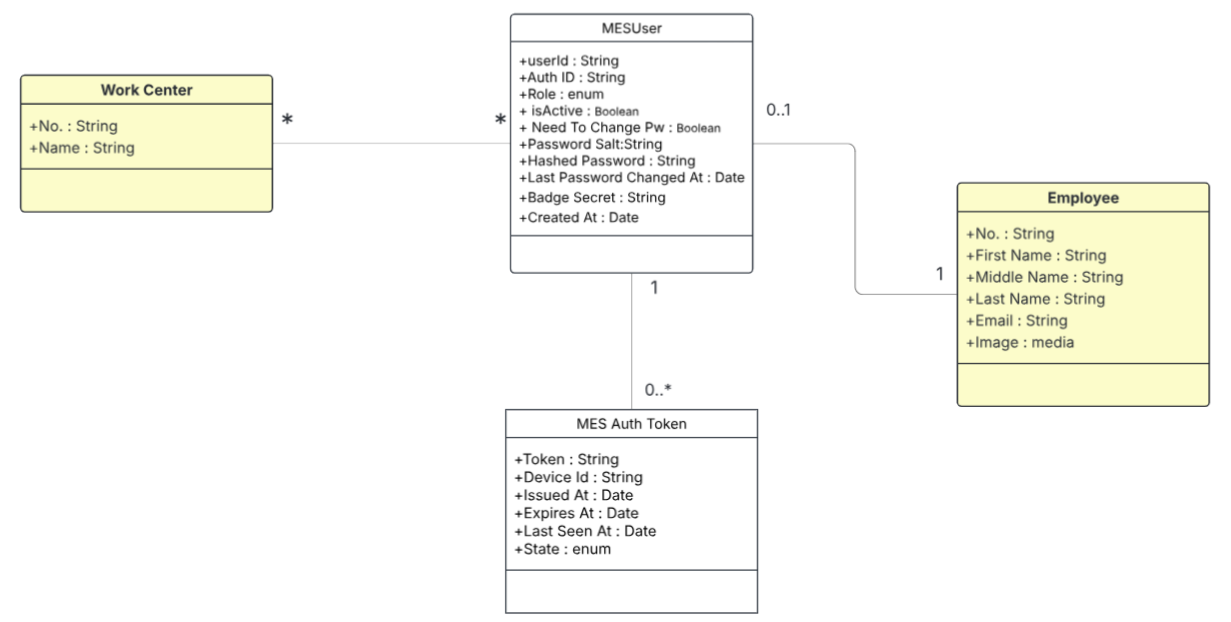
\includegraphics[width=\linewidth,keepaspectratio]{./media/MES_Sprint-1-Repport/diagrams/class/sprint1.png}
	\caption{UML Class Diagram.}
	\label{fig:s1-class-diagram}
\end{figure}


% -----------------------------------------------------------------------
\section{Implementation}
% -----------------------------------------------------------------------

\subsection{Backend Implementation}

\subsubsection{Backend Structure Overview}

The backend project structure is illustrated in Figure~\ref{fig:s1-backend-structure}.

\begin{figure}[H]
	\centering
	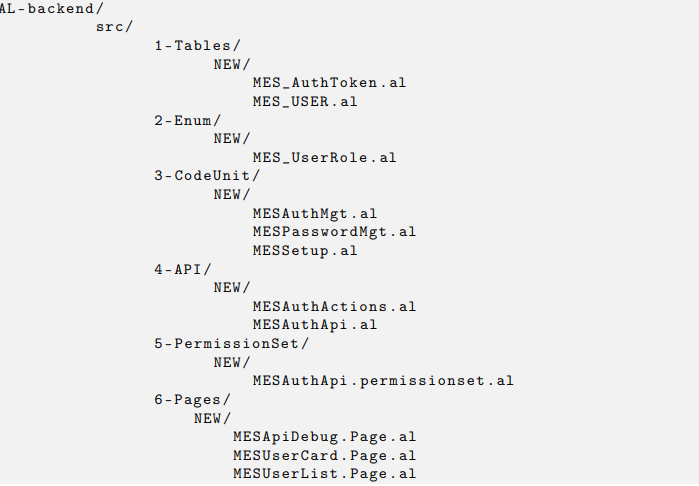
\includegraphics[width=\linewidth,keepaspectratio]{./media/MES_Sprint-1-Repport/image3.png}
	\caption{Backend project structure.}
	\label{fig:s1-backend-structure}
\end{figure}

\subsubsection{MES User Table Implementation}

The \modulename{MES User} table is implemented to store user information,
as described in Table~\ref{tab:s1-mes_user_fields}.

\begin{longtable}{@{} P{0.18\linewidth} P{0.18\linewidth} P{0.64\linewidth} @{}}
	
	\toprule
	\textbf{Name}     & \textbf{Type}                 & \textbf{Description} \\
	\midrule
	\endfirsthead
	
	\toprule
	\textbf{Name}     & \textbf{Type}                 & \textbf{Description} \\
	\midrule
	\endhead
	
	\multicolumn{3}{r}{\small Continued on next page} \\
	\endfoot
	
	\endlastfoot
	
	User Id           & Code[50]                      &                      
	Primary key. Login identifier used at the MES login prompt (e.g., \texttt{JDOE}, \texttt{OP001}). If blank on insert, a GUID-derived value is assigned automatically. \\
	\midrule
	
	Employee ID       & Code[50]                      &                      
	Foreign key to \texttt{Employee."No."}. Required for every MES account and enforced as unique (one Employee maps to one MES User). \\
	\midrule
	
	Auth ID           & Text[100]                     &                      
	Auto-generated external identifier in the form \texttt{AUTH-XXXXXXXX}. Used as the login identifier at the MES login prompt. Uniqueness enforced. \\
	\midrule
	
	Role              & Enum (\texttt{MES User Role}) &                      
	Authorization role for the MES application (e.g., Operator / Supervisor / Admin). Used to control permissions and access. \\
	\midrule
	
	%%% Work-centre assignments are stored in the separate MES User Work Center
	%%% junction table (Table 50115), not on MES User directly. Field removed. %%%
	%%%\midrule
	
	Is Active         & Boolean                       &                      
	Account enable/disable flag. If false, authentication is blocked and existing tokens are revoked when deactivated. \\
	\midrule
	
	Need To Change Pw & Boolean                       &                      
	If true, the user must change their password before using the MES application (set at creation and on forced password resets). \\
	\midrule
	
	Password Salt     & Text[64]                      &                      
	Random hex salt used in password hashing so identical passwords produce different hashes across users. \\
	\midrule
	
	Hashed Password   & Text[128]                     &                      
	Hashed password value (hex string). Passwords are never stored in plaintext; hashing uses the password plus salt. \\
	\midrule
	
	Created At        & DateTime                      &                      
	UTC timestamp set on insert only (audit trail/reporting). \\
	\midrule
	\noalign{\vskip 4pt}
	\caption{MES User (Table 50101) --- Field Dictionary}
	\label{tab:s1-mes_user_fields}
	
\end{longtable}

\subsubsection{Authentication Token Table}

The \modulename{MES Auth Token} table stores session information as described
in Table~\ref{tab:s1-mes_auth_token_fields}.

\begin{longtable}{@{} P{0.18\linewidth} P{0.18\linewidth} P{0.64\linewidth} @{}}
	
	\toprule
	\textbf{Name} & \textbf{Type} & \textbf{Description} \\
	\midrule
	\endfirsthead
	
	\toprule
	\textbf{Name} & \textbf{Type} & \textbf{Description} \\
	\midrule
	\endhead
	
	\multicolumn{3}{r}{\small Continued on next page} \\
	\endfoot
	
	\endlastfoot
	
	Token         & Guid          &                      
	Primary key. Raw GUID token presented by the client as a Bearer credential. Generated at issue time (never reused). Used for all direct token lookups (validation/logout). \\
	\midrule
	
	User Id       & Code[50]      &                      
	Foreign key to \texttt{MES User."User Id"}. Identifies the MES user who owns this session/token. Enforces referential integrity via \texttt{TableRelation}. \\
	\midrule
	
	Device Id     & Text[100]     &                      
	Optional identifier for the device that requested the token (e.g., \texttt{tablet-floor-02}, \texttt{scanner-01}). Stored for traceability/audit only; not used for validation. \\
	\midrule
	
	Issued At     & DateTime      &                      
	UTC timestamp set when the token is created. Useful for audit trail and token age inspection. \\
	\midrule
	
	Expires At    & DateTime      &                      
	UTC timestamp after which the token must be rejected even if not revoked. Set to \texttt{Issued At + TTL}. Token validation enforces \texttt{Expires At > CurrentDateTime()}. \\
	\midrule
	
	Last Seen At  & DateTime      &                      
	Updated on every successful token validation. Supports session monitoring (activity/idle detection). Not used for expiry enforcement (use \texttt{Expires At}). \\
	\midrule
	
	Revoked       & Boolean       &                      
	If true, token is explicitly invalidated and must be rejected even if not expired. Set on logout and during bulk revocation (e.g., password change, account deactivation). \\
	\midrule
	\noalign{\vskip 4pt}
	\caption{MES Auth Token (Table 50106) --- Field Dictionary}
	\label{tab:s1-mes_auth_token_fields}
	
\end{longtable}

Key points of the token design include a unique \domainterm{GUID} token,
auto-expiry after 12 hours, last activity tracking, and soft revocation.

\subsubsection{Password Management and Encryption}

The password management codeunit ensures that plaintext is never persisted. A
unique random \domainterm{salt} (64-character SHA-256 hex string) is generated per
user and the password is hashed using single-pass \domainterm{SHA-256} before storage.
Data classification attributes mark sensitive fields as \emph{Customer Content}
or \emph{System Metadata}.

Key points include: passwords are never stored in plaintext; a unique salt per user
(64 characters) is generated; \domainterm{SHA-256} hashing is applied; and data is
classified as \emph{Customer Content} or \emph{System Metadata}.

\subsubsection{Authentication Logic --- Login, Logout, and Change Password}

\textbf{Login}

The login validates the user credentials against the \modulename{MES User}
table. If the credentials are correct and the account is active, a token will
be generated and stored in the \modulename{MES Auth Token} table.

The system returns a \domainterm{JSON} login response object which includes the
generated session token, the authenticated user's role string, and a boolean
\domainterm{needChangePassword} flag consumed by the \techname{Flutter} frontend
to decide the post-login navigation target.

\textbf{Logout}

On logout, the user's session authentication token is revoked. The token
record matching the supplied session token is located in the
\modulename{MES Auth Token} table and its \texttt{Revoked} flag is set to
\texttt{true}, immediately invalidating the session (soft revocation).

\textbf{Change Password}

Changing password requires a valid authentication token, a correct current
password, and a new password that complies with security rules.

\subsection{REST API and Web Services Implementation}

To enable communication between \techname{Flutter} and
\techname{Microsoft Dynamics Business Central}, a set of \domainterm{RESTful APIs}
were implemented using AL.

\subsubsection{API Pages for MES User Management}

The \domainterm{API Page} definition for the \apiendpoint{/mesUsers} endpoint
exposes the \modulename{MES User} table as a read-only \domainterm{OData} feed.

The \domainterm{API Page} definition for the \apiendpoint{/createMesUser}
endpoint differs from the read endpoint by setting validation triggers.
\texttt{DelayedInsert\,=\,true} buffers all field values until the
complete request body has been received before committing the new
\modulename{MES User} record to the database.

Key point: the difference between these two APIs is the \domainterm{Delayed Insert} flag.
When set to \texttt{true}, it delays insertion until all fields are received,
which is required for \texttt{POST} operations. \texttt{GET} is not affected.

\subsubsection{OData Functions and Web Service Configuration}

Built \techname{MESUnboundActions} codeunit (50125): \texttt{Login()}, \texttt{Logout()}, \texttt{Me()}, \texttt{ChangePassword()}.
Exposed these functions in the \techname{MES Web Service} codeunit (50126) exposed via ODataV4.
Configured \techname{WebServices.xml} to publish \techname{MES Web Service}
(codeunit 50126) as an ODataV4 web service under the service name
\texttt{MESWebService}.

\subsection{Frontend Implementation}

The frontend of this system was developed using \techname{Flutter}. The
application is structured into four main layers: a \textbf{\domainterm{UI Layer}}
consisting of Screens and Widgets; a \textbf{\domainterm{State Management Layer}}
built on Providers; a \textbf{\domainterm{Service Layer}} for API communication;
and a \textbf{\domainterm{Model Layer}} for Data Models.


\noindent
\begin{minipage}[t]{0.6\textwidth}
	The data flow follows a unidirectional pattern from the \domainterm{UI Layer}
	through the \domainterm{State Management Layer} (\modulename{Provider} pattern)
	and \domainterm{Service Layer} to the \techname{Business Central} REST API backend,
	as illustrated in Figure~\ref{fig:s1-flutter-architecture-s1}.
	\subsubsection{Service Layer (API Communication)}

	The \domainterm{Service Layer} is responsible for handling all \domainterm{HTTP}
	communication between \techname{Flutter} and the \techname{Business Central} backend.

	Two services were implemented: the \modulename{api\_service} manages
	authentication requests such as \uilabel{login}, \uilabel{logout}, and
	\uilabel{password change}, while the \modulename{mes\_user\_service} handles MES
	user operations including fetching and creating new users.

	\textbf{\modulename{api\_service.dart}}

	The class declaration and constructor show the base URL configuration and
	\domainterm{HTTP} client initialisation used by all authentication endpoints.
	The \uilabel{login} method sends user credentials and device ID to the \apiendpoint{/login} endpoint and parses the returned session token, role, and \domainterm{needChangePassword} flag. The \uilabel{logout} method sends the active session token to the \apiendpoint{/logout} endpoint to trigger server-side token revocation.

\end{minipage}
\hfill
\begin{minipage}[t]{0.38\textwidth}
  \vspace{0pt}
  \centering
  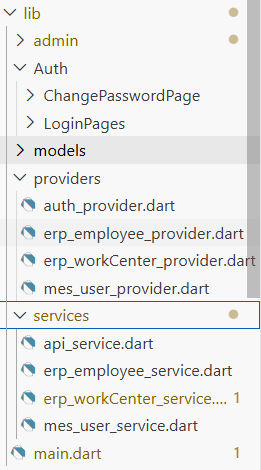
\includegraphics[width=\linewidth,keepaspectratio]{./media/MES_Sprint-1-Repport/image13.png}
  \captionof{figure}{\techname{Flutter} layered architecture.}
  \label{fig:s1-flutter-architecture-s1}
\end{minipage}

The \uilabel{change password} method submits the current password,
new password, and session token to the \apiendpoint{/changePassword} endpoint.
Shared error-handling and response-parsing utilities are used by all methods in
the service class to propagate structured exceptions to the
\domainterm{State Management Layer}.

\textbf{\modulename{mes\_user\_service.dart}}

The class declaration and \uilabel{fetch users} method send an authenticated
\domainterm{HTTP GET} request to the \apiendpoint{/mesUsers} endpoint and
deserialise the response into a list of \modulename{MesUser} model objects.
The \uilabel{create user} method sends a \domainterm{HTTP POST} request to the
\apiendpoint{/createMesUser} endpoint with the new user's role and employee
reference in the request body. The \uilabel{generate password} method and
associated response deserialisers handle the password generation endpoint and
map the \domainterm{JSON} result into the \modulename{GeneratedPassword} model.

\subsubsection{State Management Layer using Provider}

The \domainterm{Provider} pattern is implemented to ensure reactive UI updates
and centralised data handling. Two providers were implemented:
\modulename{AuthProvider}, which manages authentication state, and
\modulename{MesUserProvider}, which handles MES user data. Each provider wraps
the corresponding service layer calls and exposes reactive state (authenticated
user, user list, loading flag, error message) consumed by the \domainterm{UI Layer}
via \texttt{context.watch}.

\subsubsection{User Interface}

The \uilabel{Login Page}, shown in Figure~\ref{fig:s1-ui-login}, is the application
entry screen presented to all users on launch. It contains \uilabel{User ID} and
\uilabel{Password} input fields and a \uilabel{Login} button. Successful
authentication redirects the user to the role-appropriate dashboard.

\begin{figure}[H]
	\centering
	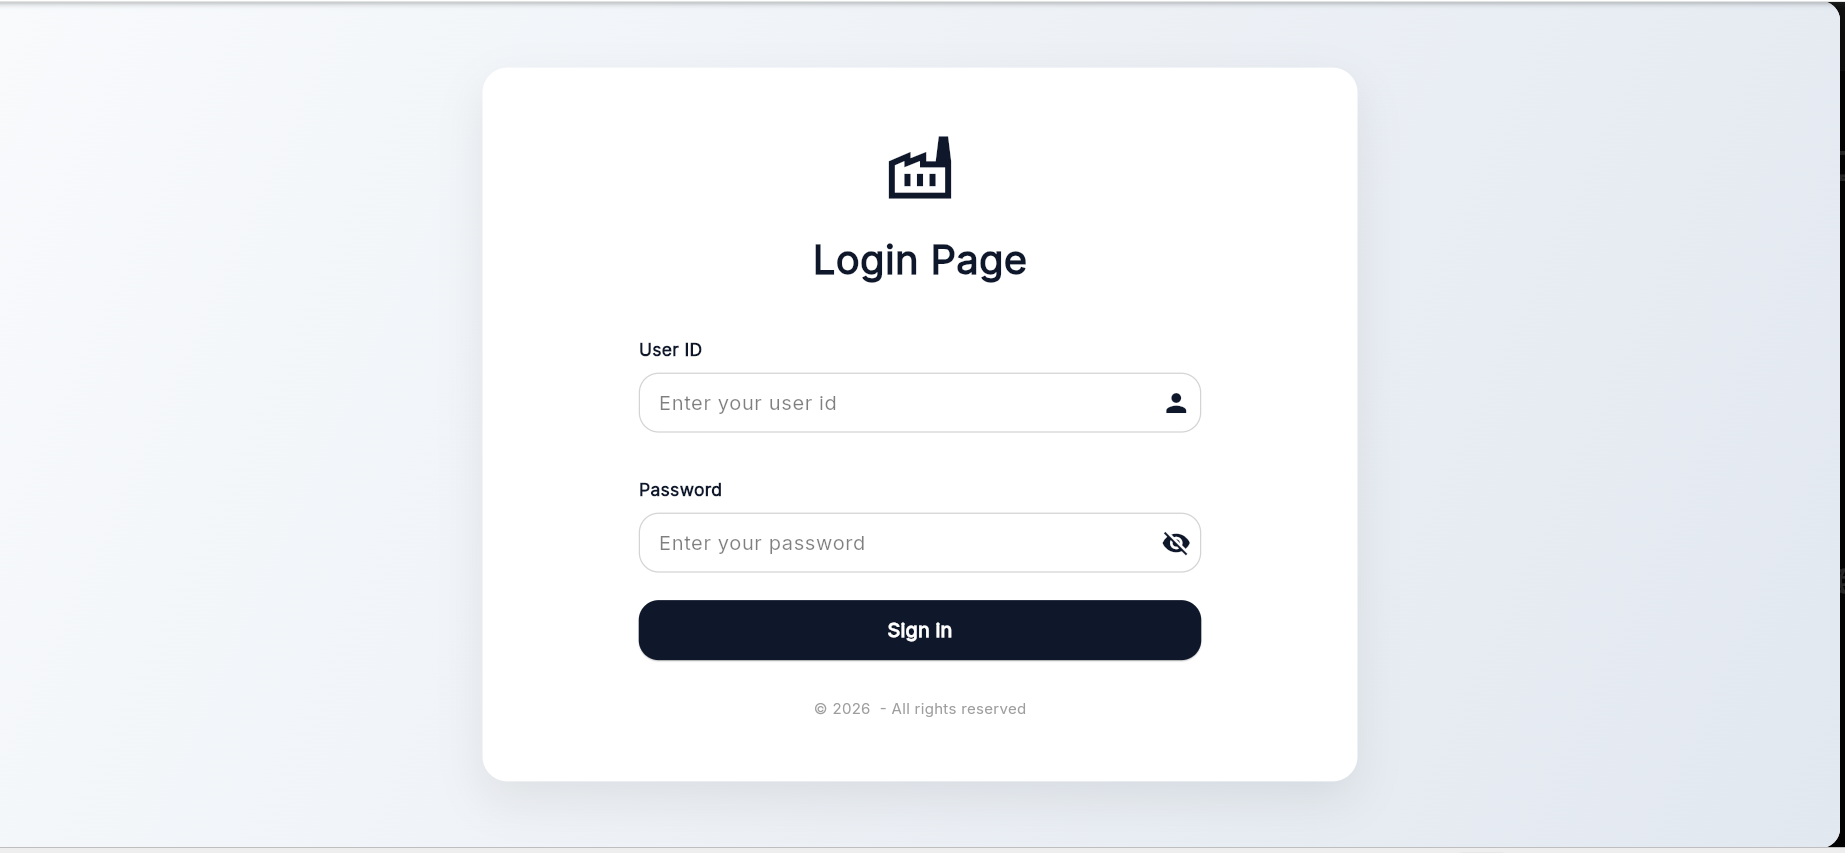
\includegraphics[width=\linewidth,keepaspectratio]{./media/MES_Sprint-1-Repport/image23.png}
	\caption{\uilabel{Login Page}.}
	\label{fig:s1-ui-login}
\end{figure}

The \uilabel{MES User List Page}, shown in Figure~\ref{fig:s1-ui-user-list}, is
the \userrole{Administrator} dashboard screen listing all registered
\domainterm{MES} users with their assigned roles and active status, providing
action buttons to assign roles or generate passwords for each employee.

\begin{figure}[H]
	\centering
	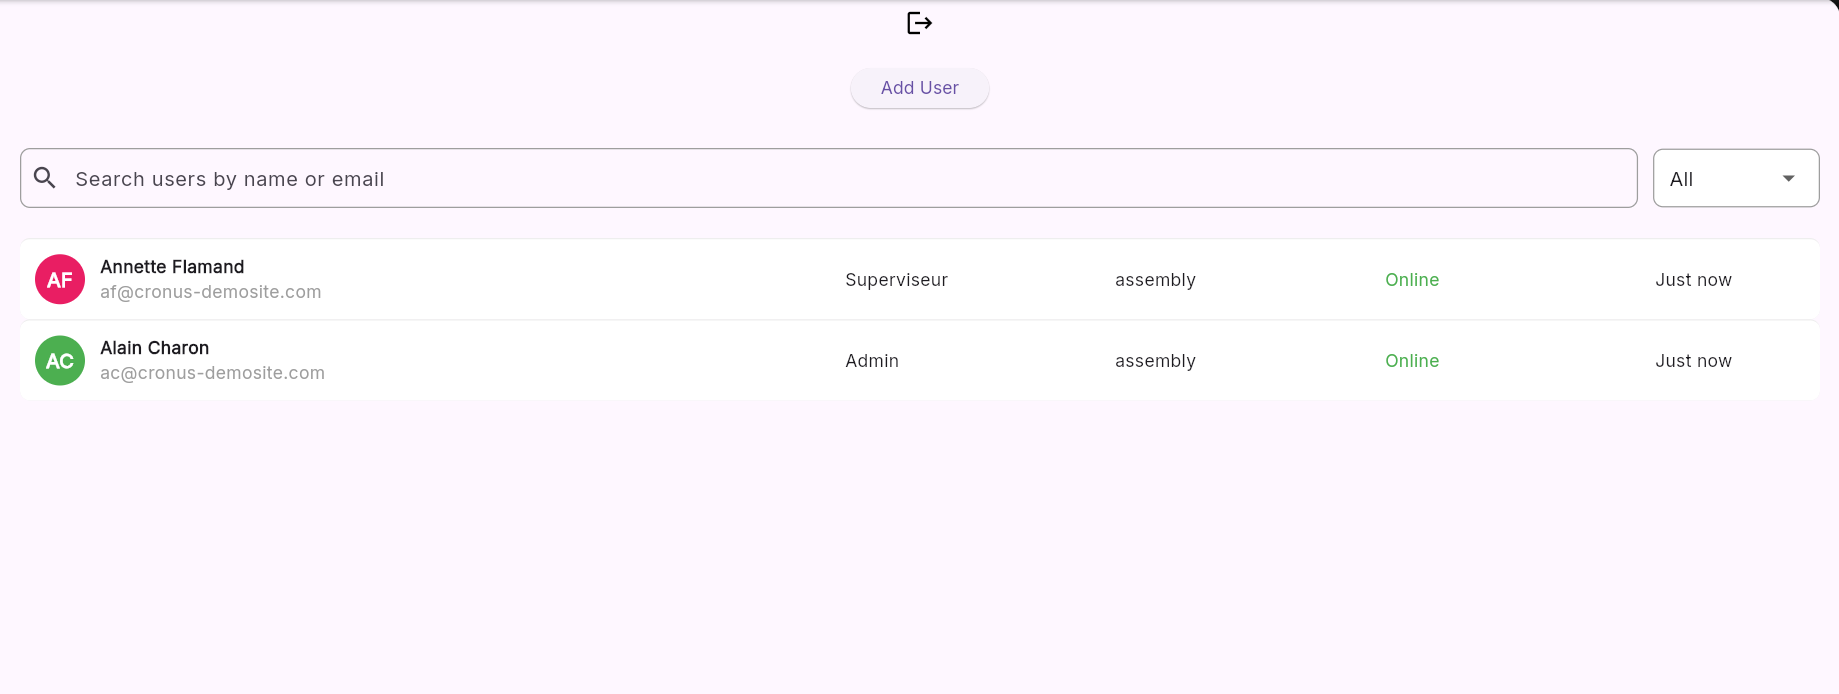
\includegraphics[width=\linewidth,keepaspectratio]{./media/MES_Sprint-1-Repport/image24.png}
	\caption{\uilabel{MES User List Page}.}
	\label{fig:s1-ui-user-list}
\end{figure}

The \uilabel{Assign MES Role Dialog}, shown in Figure~\ref{fig:s1-ui-assign-role},
is a modal dialog allowing the \userrole{Administrator} to select a
\techname{Business Central} employee record and assign them an \domainterm{MES}
role (\userrole{Operator} or \userrole{Supervisor}), creating a new
\modulename{MES User} record via the \apiendpoint{/createMesUser} endpoint.

\begin{figure}[H]
	\centering
	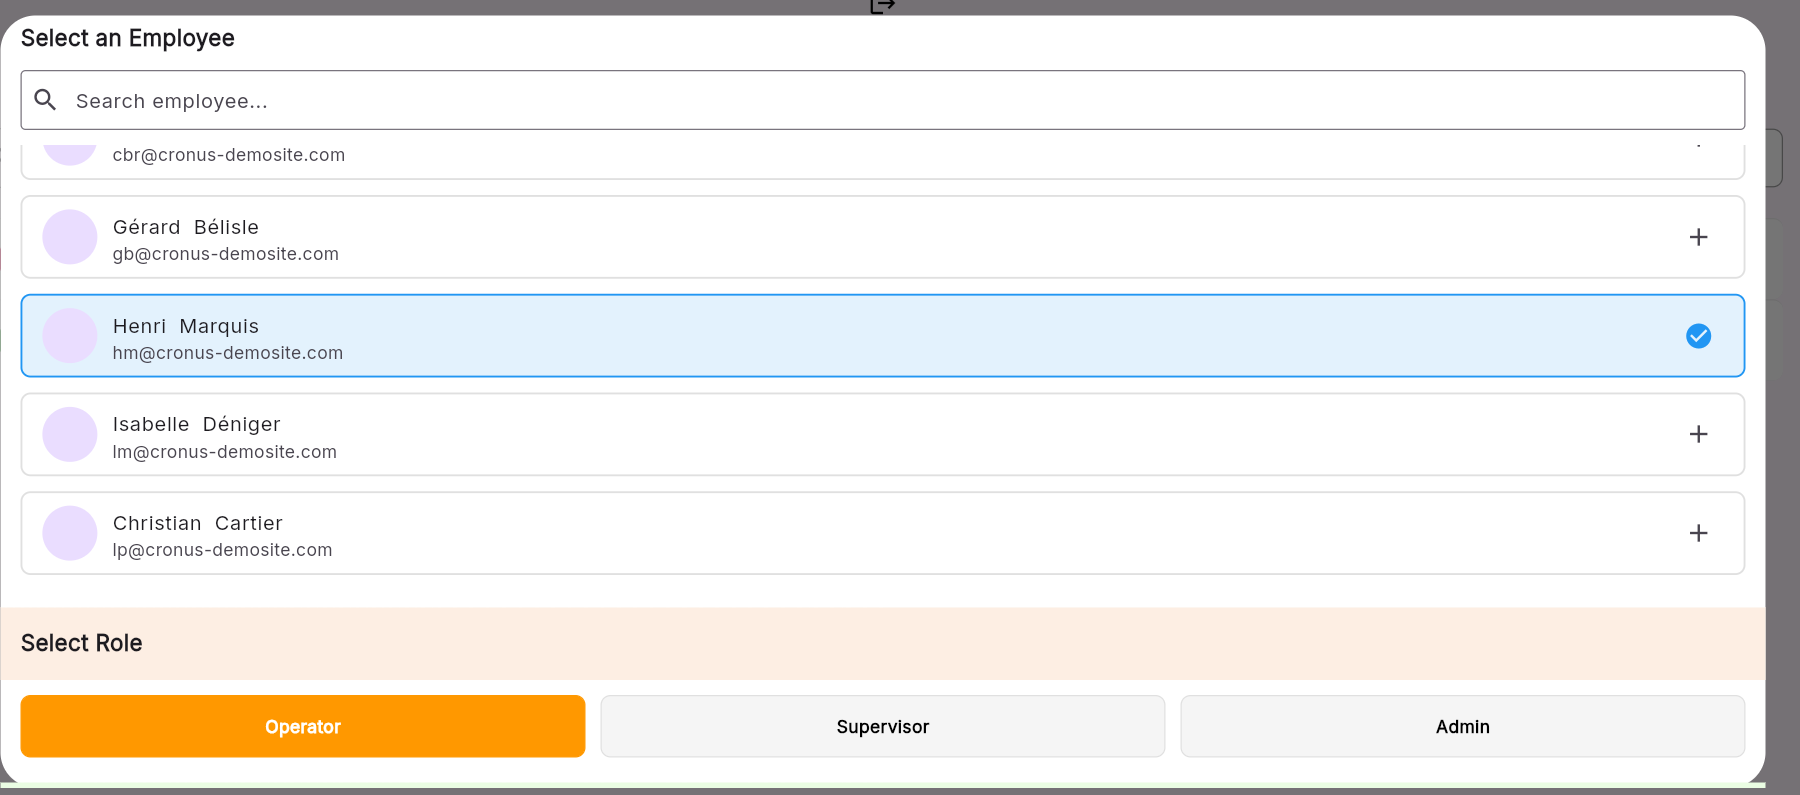
\includegraphics[width=\linewidth,keepaspectratio]{./media/MES_Sprint-1-Repport/image25.png}
	\caption{\uilabel{Assign MES Role Dialog}.}
	\label{fig:s1-ui-assign-role}
\end{figure}

The \uilabel{Generate Password Dialog}, shown in Figure~\ref{fig:s1-ui-generate-password},
is a modal dialog through which the \userrole{Administrator} triggers server-side
secure password generation for a selected \domainterm{MES} user. The generated
password is displayed once and must be communicated to the user out-of-band.

\begin{figure}[H]
	\centering
	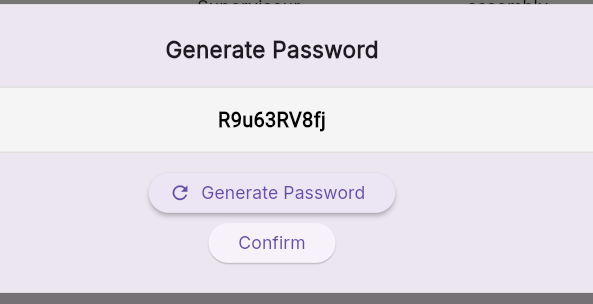
\includegraphics[width=\linewidth,keepaspectratio]{./media/MES_Sprint-1-Repport/image26.png}
	\caption{\uilabel{Generate Password Dialog}.}
	\label{fig:s1-ui-generate-password}
\end{figure}

The \uilabel{Password Generated Successfully Dialog}, shown in
Figure~\ref{fig:s1-ui-password-success}, is a confirmation dialog showing the
plaintext password to the \userrole{Administrator} for one-time transmission to
the user. The password is not stored in plaintext on the server after this point.

\begin{figure}[H]
	\centering
	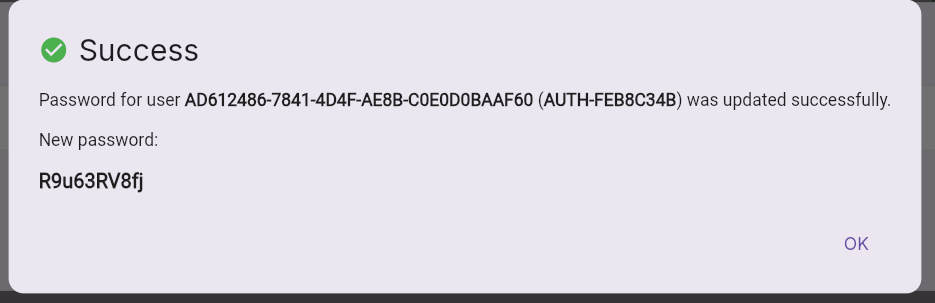
\includegraphics[width=\linewidth,keepaspectratio]{./media/MES_Sprint-1-Repport/image27.png}
	\caption{\uilabel{Password Generated Successfully Dialog}.}
	\label{fig:s1-ui-password-success}
\end{figure}

The \uilabel{Change Password Page}, shown in Figure~\ref{fig:s1-ui-change-password},
is presented to users whose \domainterm{needChangePassword} flag is \texttt{true}
after login, requiring them to enter their current password and choose a new
password before accessing the main application.

\begin{figure}[H]
	\centering
	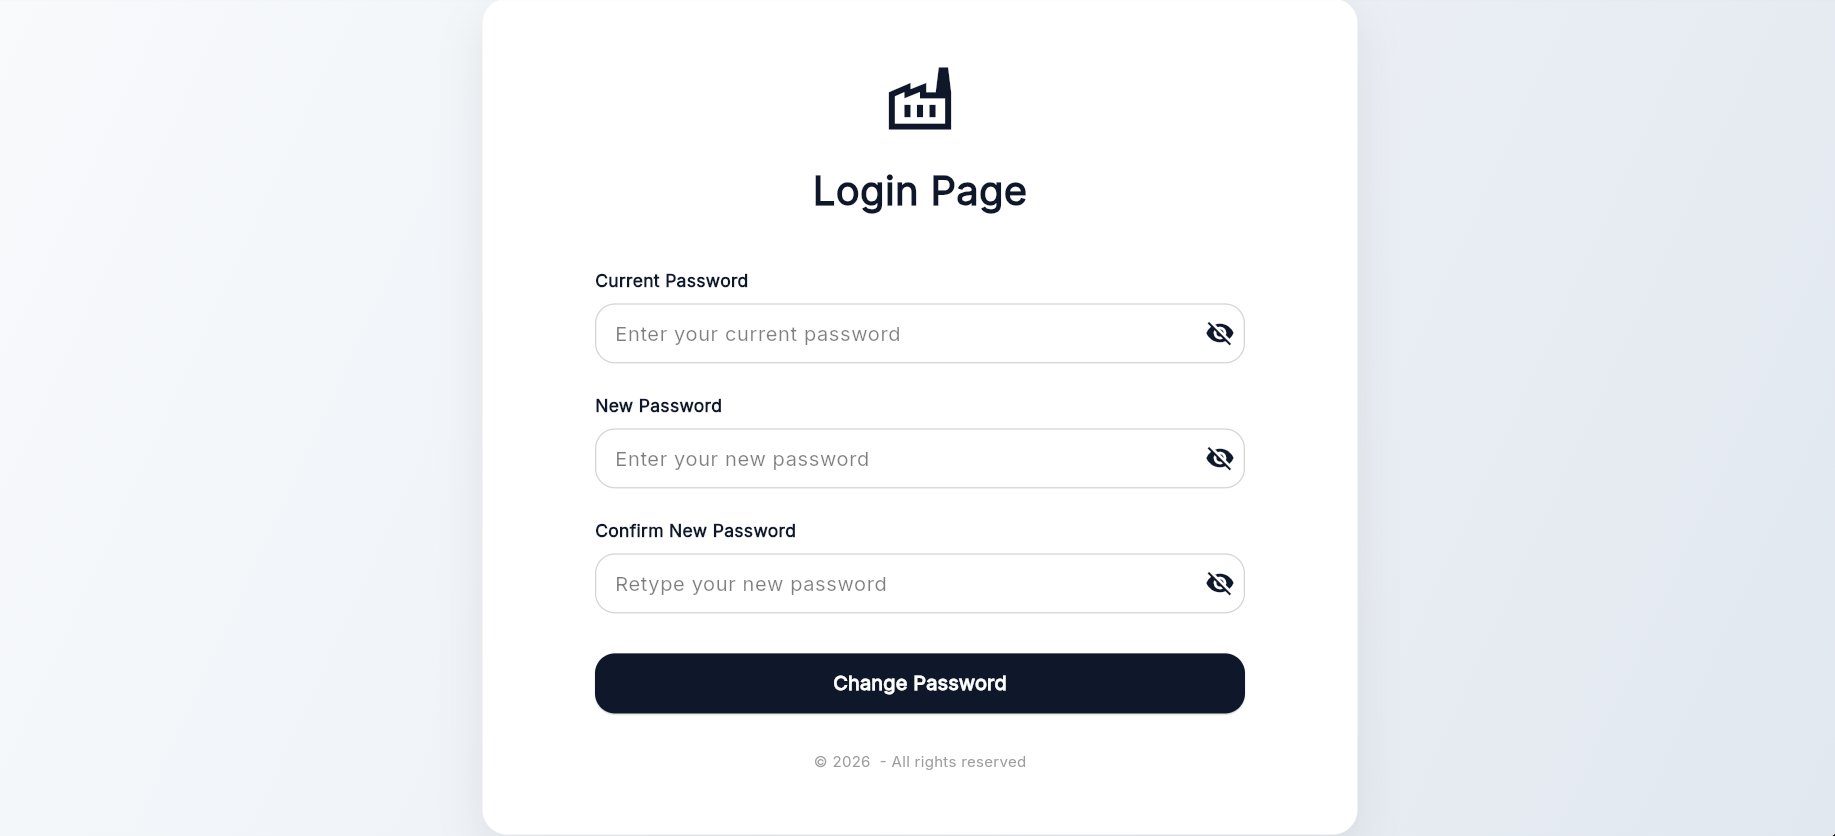
\includegraphics[width=\linewidth,keepaspectratio]{./media/MES_Sprint-1-Repport/image28.png}
	\caption{\uilabel{Change Password Page}.}
	\label{fig:s1-ui-change-password}
\end{figure}

The \uilabel{Change Role Dialog}, shown in Figure~\ref{fig:s1-ui-chRole-diag},
is a modal dialog through which the \userrole{Administrator} updates the
role and work-centre assignment of an existing \domainterm{MES} user. The
dialog pre-populates the current role and presents a three-button row
(Operator / Supervisor / Admin); selecting Admin hides the work-centre list,
selecting Operator shows a single-select list, and selecting Supervisor shows
a multi-select list. An inline error banner displays any server-side validation
failure. Tapping \uilabel{Save Changes} submits the update and revokes all
active tokens for the affected user.

\begin{figure}[H]
	\centering
	
\includegraphics[width=\linewidth,keepaspectratio]{./media/MES_Sprint-1-Repport/placeholder-image.png}
	\caption{\uilabel{Change Role Dialog}.}
	\label{fig:s1-ui-chRole-diag}
\end{figure}

The user row in the \uilabel{MES User List Page} now includes a
\texttt{PopupMenuButton} action menu accessible via a trailing icon on each row.
The menu exposes two actions: \uilabel{Change Role / Department}, which opens the
\techname{ChangeRoleDialog} described above, and \uilabel{Activate} or
\uilabel{Deactivate}, whose label switches dynamically based on the user's current
\texttt{isActive} flag. Selecting \uilabel{Deactivate} immediately revokes all
active sessions for that account; selecting \uilabel{Activate} re-enables login.

\section{Testing and Validation}
\subsection{Integration testing}
For integration testing, we chose Postman, a powerful and user-friendly tool for API evaluation. Figure~\ref{fig:s1-test-postman-fetchAllMesUsers} shows a test case for the \apiendpoint{/mesUsers} endpoint.

\begin{figure}[H]
	\centering
	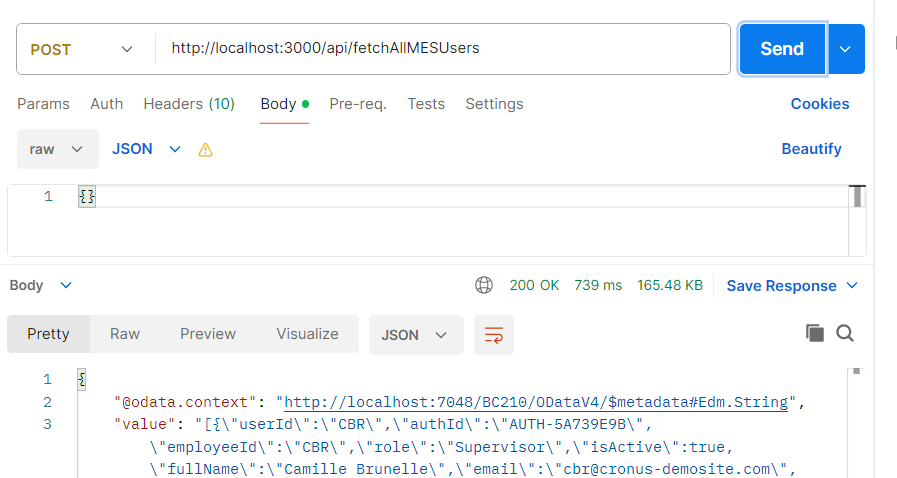
\includegraphics[width=\linewidth,keepaspectratio]{./media/MES_Sprint-1-Repport/tests/postman/fetchAllMesUsers.png}
	\caption{Postman endpoint test --- fetchAllMesUsers.}
	\label{fig:s1-test-postman-fetchAllMesUsers}
\end{figure}


% -----------------------------------------------------------------------
\phantomsection
\section*{Conclusion}
\addcontentsline{toc}{section}{Conclusion}
% -----------------------------------------------------------------------

This sprint successfully delivered a complete authentication and user management
foundation for the \domainterm{MES} application. The backend, built in
\techname{Microsoft Dynamics Business Central} using \techname{AL}, implements
secure credential validation, \domainterm{SHA-256} password hashing,
session token management with automatic expiry, and a full set of
\domainterm{RESTful} API endpoints exposed through \techname{MES Web Service}
(codeunit 50126). The \techname{Flutter} frontend provides a clean, role-aware
user experience covering login, logout, forced password change, administrator-level
user creation, role and work-centre management, and account activation control.


% ---------------------------------------------------------------------------
% Sprint 2 Machine \& Production Management
% ---------------------------------------------------------------------------
\chapter{Sprint 2 Machine \& Production Management}
\graphicspath{{./media/MES_Sprint-2-Repport/}}
\minitoc
\newpage
\minitoc
\newpage

\section*{Introduction}
\addcontentsline{toc}{section}{Introduction}

This sprint covers \textbf{Machine Monitoring, Production Order Management, and
  Operation History} in the \domainterm{MES} application, giving
\userrole{Operator}s and \userrole{Supervisor}s real-time visibility into machine
states and a full audit trail of completed operations.

It addresses three related sub-domains: live machine status tracking from
\techname{Business Central} to the \techname{Flutter} frontend, production order
management with operation lifecycle initiation, and a history view showing all
completed and cancelled operations per machine.

% ---------------------------------------------------------------------------
% 1. SPRINT BACKLOG
% ---------------------------------------------------------------------------
\section{Sprint Backlog}

This sprint covers \textbf{Domain 2:}
\textbf{\domainterm{Machine Monitoring, Production Order Management \& History}}.

% ----------------------------------------------------------
%  US-2.1
% ----------------------------------------------------------

% Guide: table captions ABOVE table; numbered as Section.Sequence
\begin{longtable}{@{} P{0.09\linewidth} P{0.34\linewidth} P{0.53\linewidth} @{}}
  \caption{Sprint Backlog}
  \label{tab:s2-sprint-backlog}\\
  \toprule
  \textbf{ID} & \textbf{User Story} & \textbf{Tasks} \\
  \midrule
  \endfirsthead
  \toprule
  \textbf{ID} & \textbf{User Story} & \textbf{Tasks} \\
  \midrule
  \endhead
  \multicolumn{3}{r}{\small Continued on next page} \\
  \endfoot
  \bottomrule
  \endlastfoot
  
  \textbf{US-2.1}
  & As an \userrole{Operator} or \userrole{Supervisor}, I need to see the list
  of machines in my work centre with their current status so that I can see
  which machines are currently active.
  & \noindent\textit{Business Central (AL):}
  \begin{itemize}[noitemsep, topsep=0pt, partopsep=0pt, leftmargin=*]
  \item Created table \techname{MES MachineStatus}.
  \item Created enum \techname{MES Machine Status}.
  \item Created function \texttt{FetchMachines()} in codeunit \techname{MES Machine Fetch}.
  \item Exposed \texttt{FetchMachines()} through codeunit \techname{MES Web Service}.
  \item Created page \techname{MES Machine List}.
  \end{itemize}
  \\ & &
  \noindent\textit{Flutter:}
  \begin{itemize}[noitemsep, topsep=0pt, partopsep=0pt, leftmargin=*]
  \item Created model \techname{MachineModel}.
  \item Created service \techname{MESMachineListService} to consume the \texttt{FetchMachines()} API.
  \item Created provider \techname{MesMachinesProvider}.
  \item Created page \techname{MachineListPage}.
  \item Created widget \techname{MachineCard}.
  \item Implemented automatic machine list refresh in \techname{MESMachineListService}.
  \end{itemize}\\
  \midrule
  \textbf{US-2.2}
  & As an \userrole{Operator} or \userrole{Supervisor}, I need to view the
  production orders assigned to a machine so that I know what work needs
  to be done.
  & \noindent\textit{Business Central (AL):}
  \begin{itemize}[noitemsep, topsep=0pt, partopsep=0pt, leftmargin=*]
    \item Created function \texttt{getMachineOrders()} in codeunit \techname{MES Machine Fetch}.
    \item exposed  \texttt{getMachineOrders()} in codeunit \techname{MES Web Service}.
  \end{itemize}
\\ & &
  \noindent\textit{Flutter:}
  \begin{itemize}[noitemsep, topsep=0pt, partopsep=0pt, leftmargin=*]
    \item Created model \techname{MachineOrderModel}.
    \item Created service \techname{ErpMachineOrdersService} to consume the \texttt{getMachineOrders()} API.
    \item Created provider \techname{MachineordersProvider}.
    \item Created page \techname{MachineOrderPage}.
    \item Created widget \techname{OrderCard}.
    \item Created model \techname{BadgeStyle}.
  \end{itemize}\\
  \midrule
  \textbf{US-2.3}
  & As an \userrole{Operator} or \userrole{Supervisor}, I need to start a
  production operation so that the system records that the order has begun.
  & \noindent\textit{Business Central (AL):}
  \begin{itemize}[noitemsep, topsep=0pt, partopsep=0pt, leftmargin=*]
    \item Created table \techname{MES Operation state}.
    \item Created enum \techname{MES Operation Status}.
    \item Created function \texttt{TryStartOperation()} in codeunit \techname{MES Machine Validation}.
    \item Created function \texttt{InsertMESOperation()} in codeunit \techname{MES Machine Write}.
    \item Exposed \texttt{InsertMESOperation()} through codeunit \techname{MES Web Service}.
    \item Created page \techname{MES Operations}.
  \end{itemize}

  \noindent\textit{Flutter:}
  \begin{itemize}[noitemsep, topsep=0pt, partopsep=0pt, leftmargin=*]
    \item Implemented \techname{ErpMachineOrdersService} that Consumes the \texttt{startOperation} API.
    \item Implement \techname{MachineordersProvider} to manage its state.
    \item Implemented start operation action handling in \techname{ActionButtons}.
    \item Implemented automatic navigation to \techname{OrdersProgressionPage}
  \end{itemize}\\
  \midrule
  \textbf{US-2.4}
  & As a \userrole{Supervisor} or \userrole{Operator}, I need to monitor the
  current status of all active operations on a machine so that I can follow
  the progress of each order.
  & \noindent\textit{Business Central (AL):}
  \begin{itemize}[noitemsep, topsep=0pt, partopsep=0pt, leftmargin=*]
    \item Created function \texttt{fetchMachineOperationStatus()} in codeunit \techname{MES Machine Fetch}.
    \item Exposed \texttt{fetchMachineOperationStatus()} through codeunit \techname{MES Web Service}.
  \end{itemize}
\\ & &
  \noindent\textit{Flutter:}
  \begin{itemize}[noitemsep, topsep=0pt, partopsep=0pt, leftmargin=*]
    \item Updated \techname{ErpMachineOrdersService}to Consume the \texttt{fetchMachineOperationStatus}.
    \item Created model \techname{OperationStatusStyle}.
    \item Created page \techname{OrdersProgressionPage}.
    \item Created the widgets \techname{OperationCard}, \techname{OperationStatusBadge}, widget \techname{OperationInfoGrid}, and \techname{OperationProgressBar}.
    \item Implemented automatic refresh for operation status monitoring.
  \end{itemize} \\
  \midrule
  \textbf{US-2.5}
  & As an \userrole{Operator} or \userrole{Supervisor}, I need a tabbed view
  for a machine so that I can navigate between pending orders and active
  operation progress without leaving the machine context.
  & \noindent\textit{Flutter:}
  \begin{itemize}[noitemsep, topsep=0pt, partopsep=0pt, leftmargin=*]
    \item Created page \techname{MachineMainPage}.
    \item Created the widgets \techname{TopNavigationBar} and \techname{NavButton}.
    \item Implemented tab navigation in \techname{MachineMainPage}.
    \item Implemented navigation from \techname{MachineCard} to \techname{MachineMainPage}.
  \end{itemize} \\
  \midrule
  \textbf{US-2.6}
  & As an \userrole{Operator} or \userrole{Supervisor}, I need to filter and
  sort production orders so that I can quickly find the most relevant work.
  & \noindent\textit{Flutter:}
  \begin{itemize}[noitemsep, topsep=0pt, partopsep=0pt, leftmargin=*]
    \item Created widget \techname{GlobalSearchBar}.
    \item Implemented order search, filtering, and sorting in \techname{MachineOrderPage}.
  \end{itemize} \\
  \midrule
  \textbf{US-2.7}
  & As a \userrole{Supervisor} or \userrole{Operator}, I need to view the
  history of completed operations for a machine so that I can audit past
  production.
  & \noindent\textit{Business Central (AL):}
  \begin{itemize}[noitemsep, topsep=0pt, partopsep=0pt, leftmargin=*]
    \item Created function \texttt{fetchOperationsStatusAndProgress()} in codeunit \techname{MES Machine Fetch}.
    \item Exposed \texttt{fetchOperationsStatusAndProgress()} in codeunit \techname{MES Web Service}.
  \end{itemize}
\\ & &
  \noindent\textit{Flutter:}
  \begin{itemize}[noitemsep, topsep=0pt, partopsep=0pt, leftmargin=*]
    \item Updated \techname{ErpMachineOrdersService} to consume the \texttt{fetchMachineOperationStatusAndProgress} API.
    \item Updated \techname{MachineordersProvider} to manage its state.
    \item Created page \techname{MachineHistoryPage}.
    \item Created the widgets \techname{HistoryCard}, \techname{HistoryBadgeAndId}, and \techname{HistoryInfoGrid}.
    \item Implemented history search and sorting in \techname{MachineHistoryPage}.
    \item Implemented navigation from \techname{HistoryCard} to \techname{OperationDetailPage}.
  \end{itemize}\\  
\end{longtable}

% ---------------------------------------------------------------------------
% 2. BUSINESS RULES
% ---------------------------------------------------------------------------
\section{Business Rules}

\Needspace{12\baselineskip}
\begin{longtable}{@{} P{0.30\linewidth} P{0.65\linewidth} @{}}
	\caption{Business Rules}
	\label{tab:s2-Business-Rules}\\
	\toprule
	\textbf{ID: Business Rule} & \textbf{Description} \\
	\midrule
	\endfirsthead
	\toprule
	\textbf{ID: Business Rule} & \textbf{Description} \\
	\midrule
	\endhead
	\multicolumn{2}{r}{\small Continued on next page} \\
	\endfoot
	\bottomrule
	\endlastfoot
	
	\multicolumn{2}{@{}l}{\textbf{Machine Status Rules}} \\
	\midrule
	
	\businessrule{BR-MCH-001}: Machine Status Tracking &
	\begin{itemize}
	  \item Machine status is stored as an append-only log in the
	        \modulename{MES Machine Status} table; the latest record per machine
	        represents the current state.
	  \item Valid statuses are \domainterm{Idle}, \domainterm{Starting}, and
	        \domainterm{OutOfOrder}.
	  \item The \techname{Flutter} frontend polls the status endpoint every 5 seconds
	        via a \domainterm{Stream} to maintain a live view.
	\end{itemize} \\
	\midrule
	
	\businessrule{BR-MCH-002}: Work Centre Scoping &
	\begin{itemize}
	  \item The machine list is always filtered to the work centre stored in the
	        authenticated user's session token response.
	  \item An \userrole{Operator} or \userrole{Supervisor} can only see machines
	        belonging to their assigned work centre.
	\end{itemize} \\
	\midrule
	
	\multicolumn{2}{@{}l}{\textbf{Operation Lifecycle Rules}} \\
	\midrule
	
	\businessrule{BR-OPS-001}: Start Operation Validation &
	\begin{itemize}
	  \item Only routing lines with status \domainterm{Released} may be started.
	  \item An operation that already has a \domainterm{Running} record may not be
	        started again.
	  \item A machine may not run more than one operation at a time; attempting to
	        start a second operation on a busy machine is rejected with a descriptive
	        error message.
	\end{itemize} \\
	\midrule
	
	\businessrule{BR-OPS-002}: Immutable Operation History &
	\begin{itemize}
	  \item Each state transition (start, pause, resume) inserts a \emph{new} record
	        into \modulename{MES Operation Status} rather than modifying an existing
	        one, preserving a full audit trail.
	  \item The latest status for a given (machine, order, operation) triple is
	        determined by sorting on \modulename{Last Updated At} descending and
	        taking the first record.
	\end{itemize} \\
	\midrule
	
	\businessrule{BR-OPS-003}: Active Operation Query &
	\begin{itemize}
	  \item When fetching active operations for a machine, the backend groups records
	        by (production order, operation) and returns only those whose most recent
	        record has status \domainterm{Running} or \domainterm{Paused}.
	  \item Operations whose latest record is \domainterm{Finished} are excluded from
	        the active list.
	\end{itemize} \\
	\midrule
	
	\multicolumn{2}{@{}l}{\textbf{History Query Rules}} \\
	\midrule
	
	\businessrule{BR-HIST-001}: History Scope &
	\begin{itemize}
	  \item The History tab queries \modulename{fetchOperationsStatusAndProgress}
	        with \texttt{fetchFinished = true}, returning only \domainterm{Finished}
	        and \domainterm{Cancelled} executions.
	  \item The earliest \domainterm{Running} status timestamp is resolved as
	        \texttt{startDateTime}; the first \domainterm{Finished} or
	        \domainterm{Cancelled} timestamp as \texttt{endDateTime}.
	  \item History is loaded as a one-shot \texttt{Future} on page open; it is
	        not polled, as completed records are immutable.
	\end{itemize} \\
\end{longtable}

% ---------------------------------------------------------------------------
% 3. DESIGN
% ---------------------------------------------------------------------------
\section{Design}


\subsection{Use Case Diagram}

\begin{figure}[H]
  \centering
  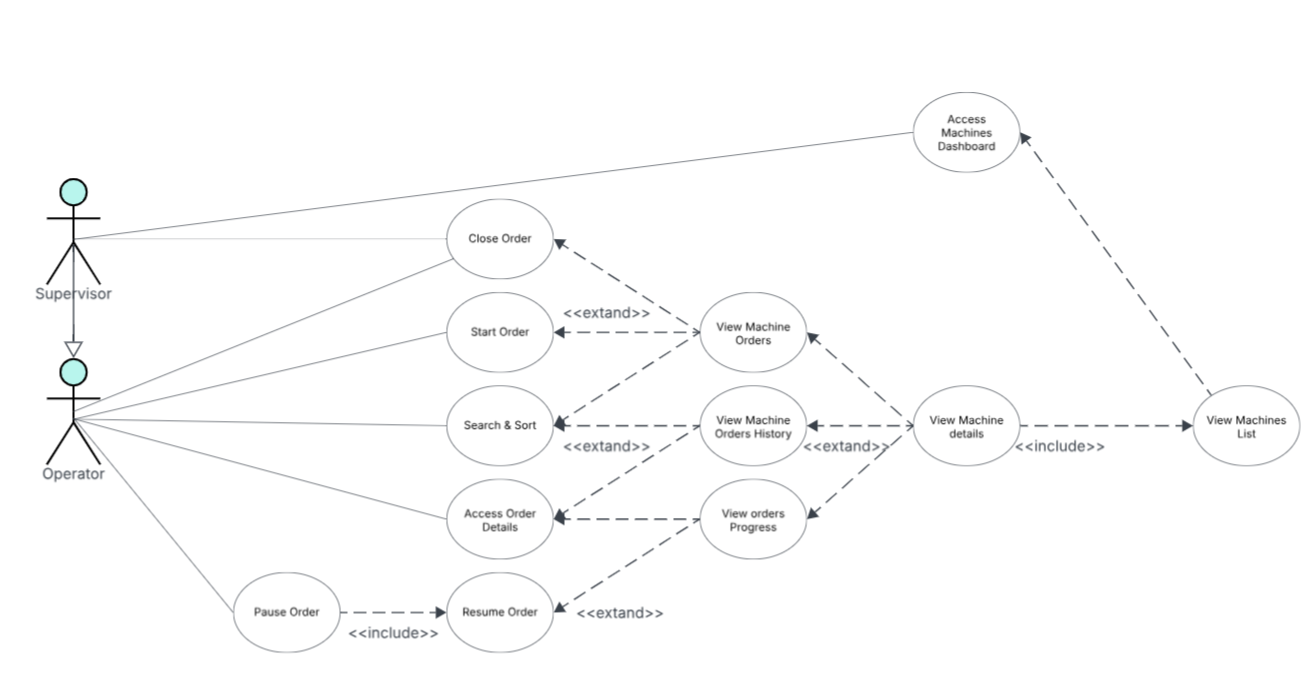
\includegraphics[width=6in]{./media/MES_Sprint-2-Repport/diagrams/useCase/sprint2.png}
  \caption{UML Use Case Diagram --- Machine \& Production Management.}
  \label{fig:s2-use-case-diagram-s2}
\end{figure}


The UML Use Case Diagram (Figure~\ref{fig:s2-use-case-diagram-s2}) shows the two
primary actors (\userrole{Operator} and \userrole{Supervisor}) and their
interactions with the machine monitoring, production order management, and history
subsystem. In addition to viewing machines, browsing orders, and managing operation
lifecycle transitions, the diagram includes the \uilabel{View Operation History}
use case, which allows both actors to access the completed and cancelled operation
log for any machine in their work centre.

\subsection{Textual Use Case Description}

The following table (Table~\ref{tab:s2-use-case-start-operation}) provides the detailed
textual description of the \textit{Start Operation} use case.

\Needspace{10\baselineskip}
\begin{longtable}{@{} P{0.21\linewidth} P{0.75\linewidth} @{}}
  
  \caption{Textual Use Case Description --- Start Operation}
  \label{tab:s2-use-case-start-operation}\\
  \toprule
  \endfirsthead
  
  \midrule
  \endhead
  
  \midrule
  \multicolumn{2}{r}{\small Continued on next page}\\
  \endfoot
  
  \bottomrule
  \endlastfoot
  
  \textbf{Use Case Name}  & Start Operation     \\
  \midrule
  \textbf{Primary Actor}  & \userrole{Operator} \\
  \midrule
  \textbf{Preconditions}  &                     
  \begin{itemize}[noitemsep, topsep=0pt, partopsep=0pt, leftmargin=*]
  \item The \userrole{Operator} is authenticated and has a valid session token.
  \item The target routing line has status \domainterm{Released}.
  \item No other operation is currently \domainterm{Running} on the same machine.
  \item The operation has not already been started (no existing
  \domainterm{Running} record for this order/operation pair).
  \end{itemize} \\
  \midrule
  
  \textbf{Postconditions} &                     
  \begin{itemize}[noitemsep, topsep=0pt, partopsep=0pt, leftmargin=*]
  \item A new \modulename{MES Operation Status} record is inserted with status
  \domainterm{Running} and the current \domainterm{UTC} timestamp.
  \item The \uilabel{Operations Progress} tab reflects the new running operation
  within the next polling cycle.
  \item If any precondition fails, a descriptive error dialog is shown to the
  operator and no record is inserted.
  \end{itemize} \\
  \midrule
  
  \textbf{Main Scenario}  &                     
  \begin{enumerate}[noitemsep, topsep=0pt, partopsep=0pt, leftmargin=*]
  \item The \userrole{Operator} navigates to the \uilabel{Machine List Page} and
  selects a machine.
  \item The system displays the \uilabel{Machine Orders Page} listing all
  applicable production orders.
  \item The \userrole{Operator} locates a \domainterm{Released} order and taps
  \uilabel{Start Order}.
  \item The frontend sends a \domainterm{POST} request to
  \apiendpoint{MESMachinesActionsEndpoints\_startOperation}.
  \item The backend validates all preconditions (\businessrule{BR-OPS-001}).
  \item On success, a \modulename{MES Operation Status} record is inserted.
  \item The frontend navigates to the \uilabel{Orders Progression Page}.
  \end{enumerate} \\
  
\end{longtable}

\subsection{Sequence Diagrams}

The following sequence diagrams illustrate the communication flow between the
\techname{Flutter} frontend, the \techname{Business Central} OData layer, and the
\techname{AL} business logic for each machine and operation flow.

Figure~\ref{fig:s2-seq-fetch-machines} shows the fetch machines flow.
Figure~\ref{fig:s2-seq-machine-orders} illustrates the get machine orders flow.
Figure~\ref{fig:s2-seq-start-operation} depicts the start operation flow.
Figure~\ref{fig:s2-seq-fetch-ops-status} presents the fetch operations status flow.

\begin{figure}[H]
  \centering
  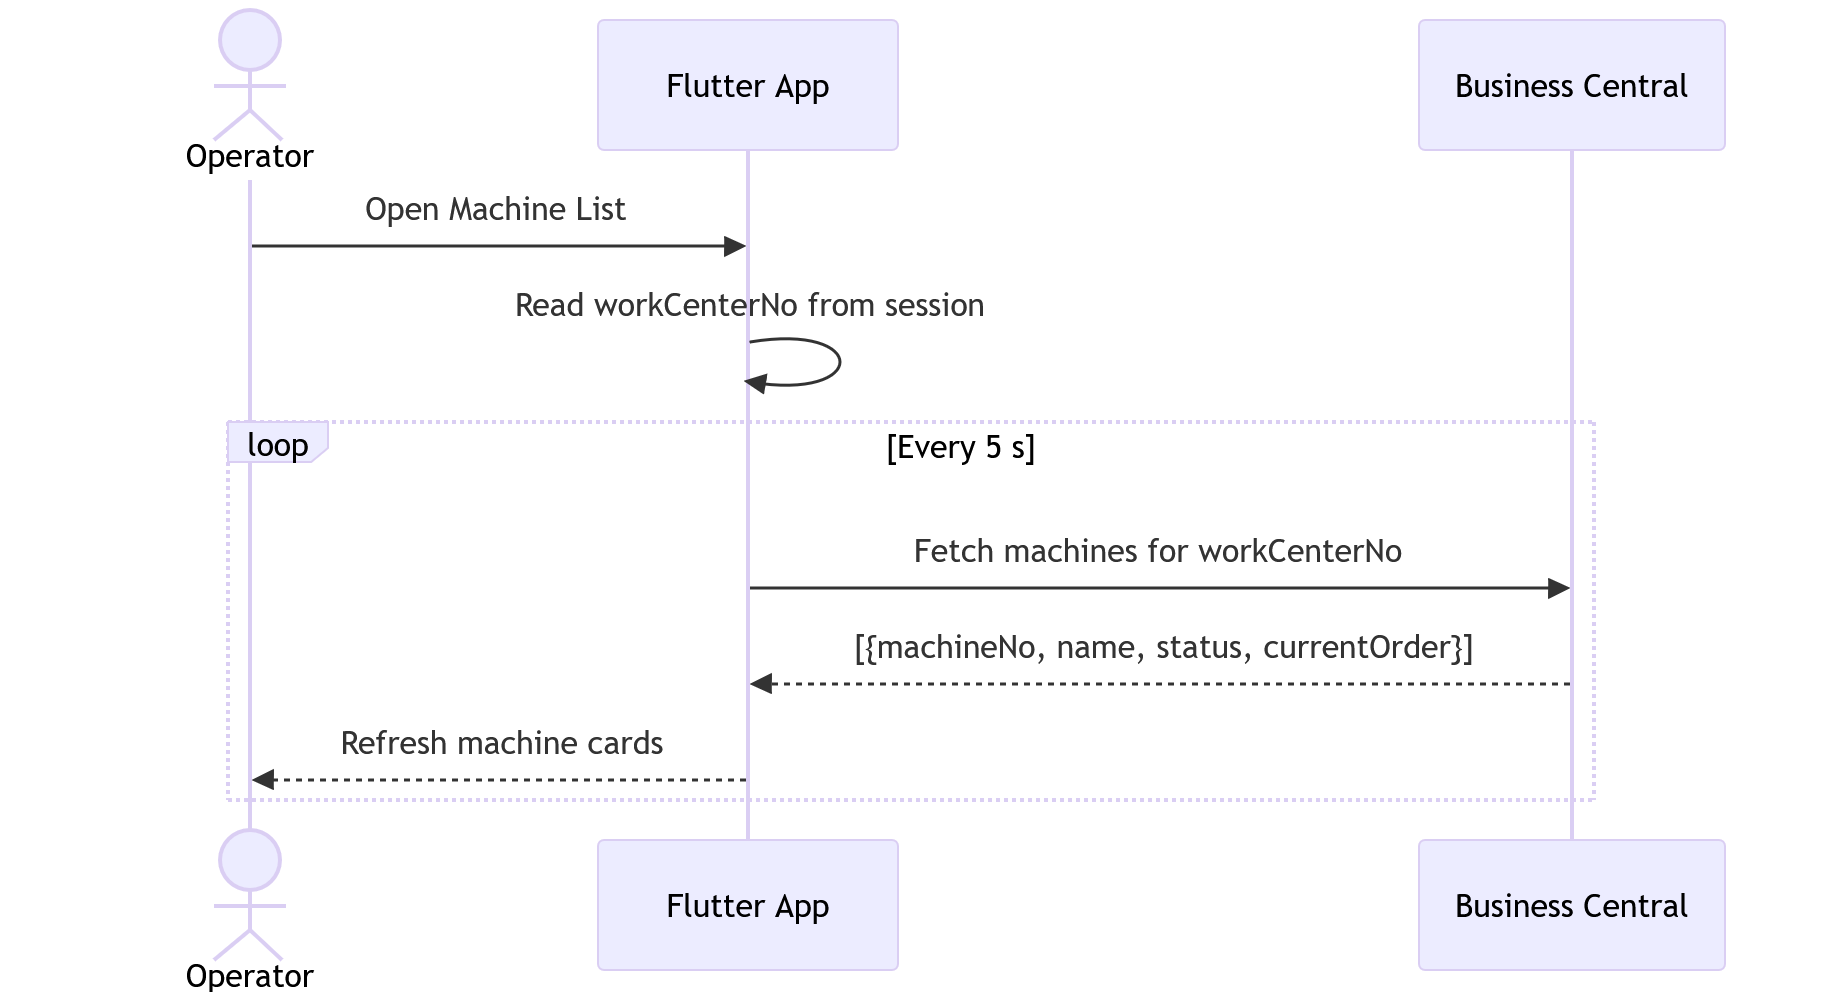
\includegraphics[width=\linewidth,keepaspectratio]{./media/MES_Sprint-2-Repport/diagrams/sequence/fetch-machines.png}
  \caption{SD-09: Fetch Machines.}
  \label{fig:s2-seq-fetch-machines}
\end{figure}

%=====SD-09==========================================================
% sequenceDiagram
%     actor User
%     participant Flutter
%     participant AL
%     participant BC

%     rect rgb(220,235,255)
%         Note over User,BC: ref SD-01 — user is logged in workCenterIds resolved from userData;
%     end

%     loop Every 5 seconds per work center
%         Flutter->>AL: FetchMachines request
%         AL->>BC: Filter Machine Center by workCenterNo
%         BC-->>AL: machine list
%         loop For each machine
%             AL->>BC: Get latest MES Machine Status row
%             BC-->>AL: machine data
%             AL->>BC: Get Work Center name
%             BC-->>AL: name
%         end
%         AL-->>Flutter: request response
%         Flutter->>Flutter: Rebuild MachineCard grid
%         Flutter-->>User: Updated machine list
%     end
%====================================================================

\begin{figure}[H]
  \centering
  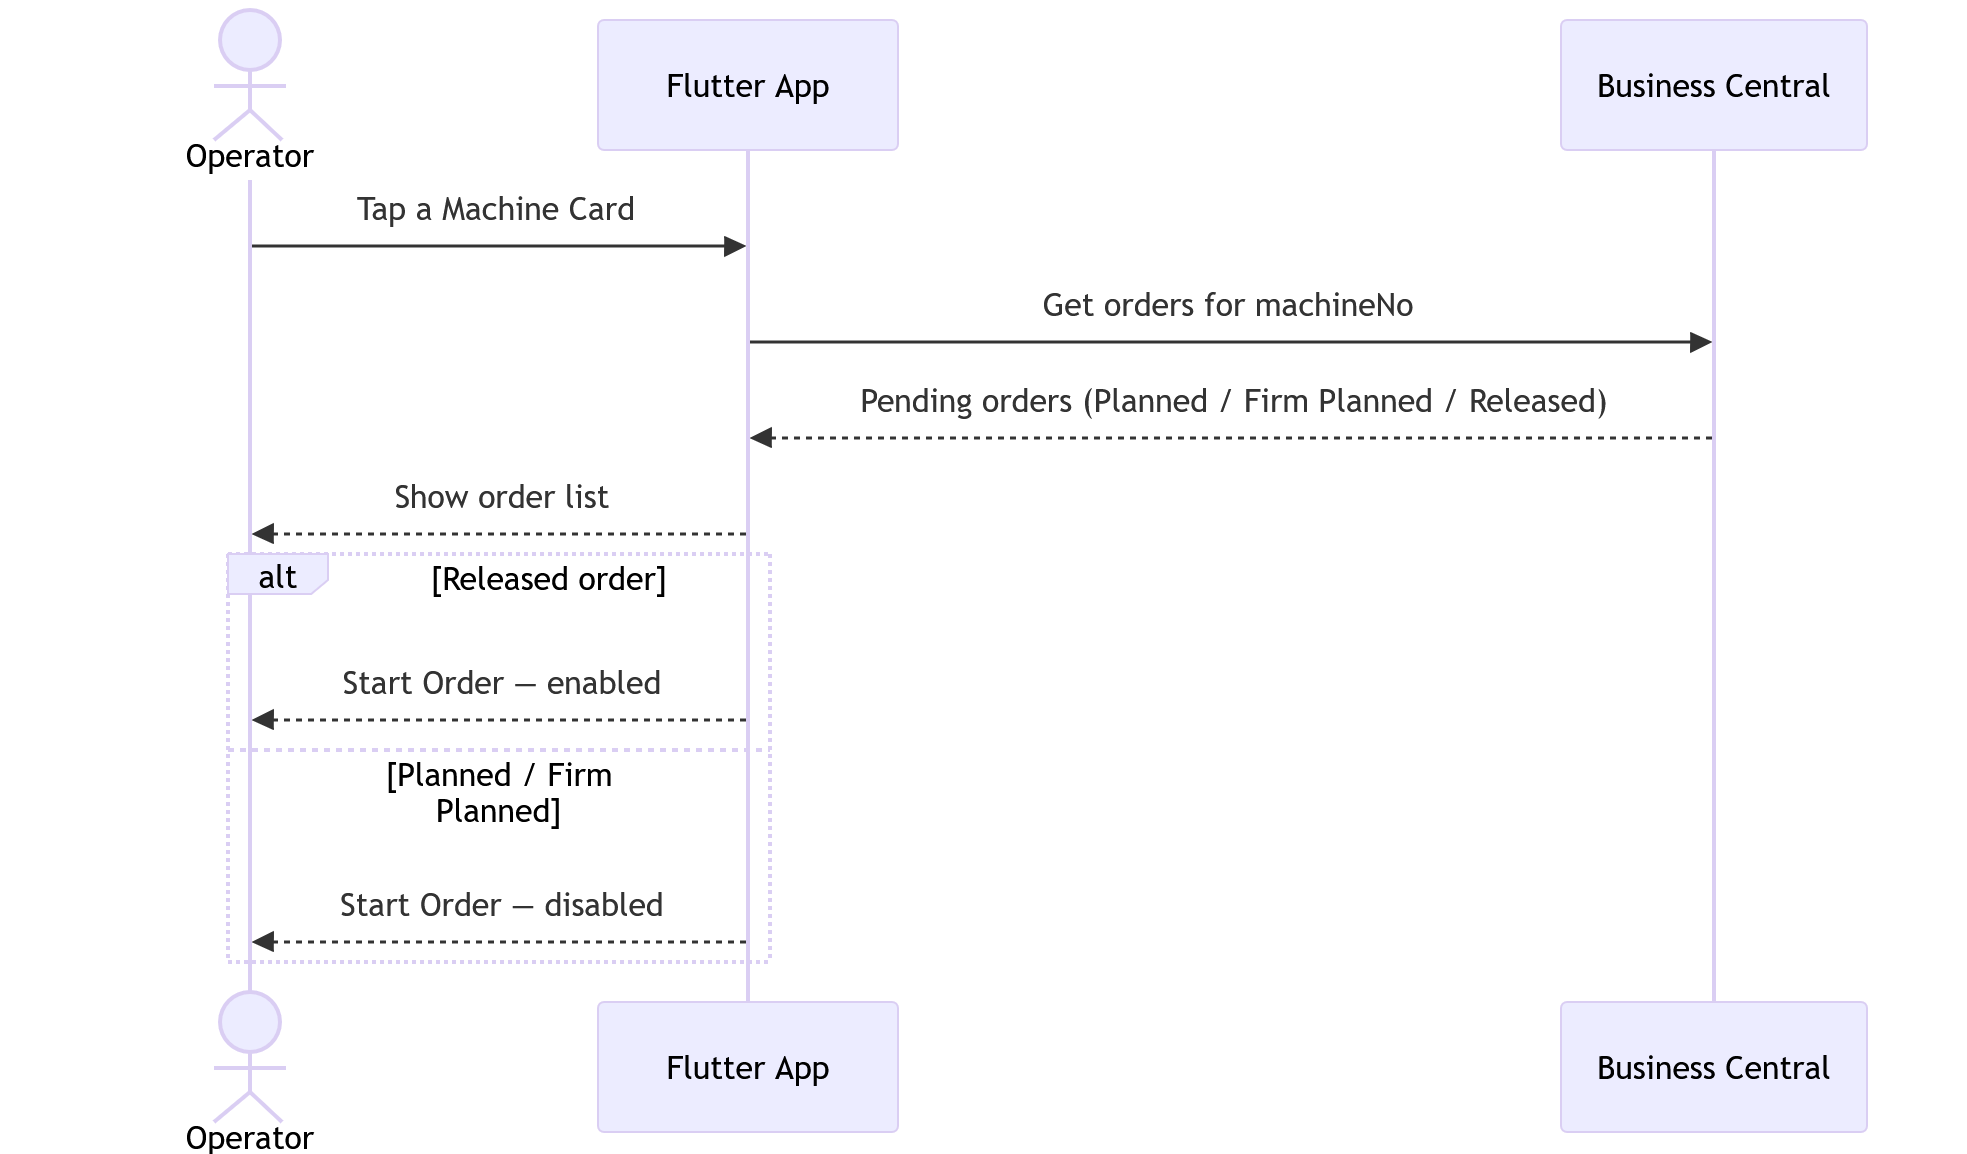
\includegraphics[width=\linewidth,keepaspectratio]{./media/MES_Sprint-2-Repport/diagrams/sequence/waiting-orders.png}
  \caption{SD-10: Get Machine Orders.}
  \label{fig:s2-seq-machine-orders}
\end{figure}

%=====SD-10==========================================================
% sequenceDiagram
%     actor User
%     participant Flutter
%     participant AL
%     participant BC

%     rect rgb(220,235,255)
%         Note over User,BC: ref SD-01 — user is logged in
%     end

%     User->>Flutter: Open Orders tab
%     Flutter->>AL: getMachineOrders request
%     AL->>BC: Filter ProdOrderRoutingLine
%     BC-->>AL: routing lines
%     loop For each routing line
%         AL->>BC: Check if operation started - skip if yes
%         AL->>BC: Get ProdOrderLine
%         BC-->>AL: line detail
%     end
%     AL-->>Flutter: orders data
%     Flutter-->>User: OrderCard list
%====================================================================

\begin{figure}[H]
  \centering
  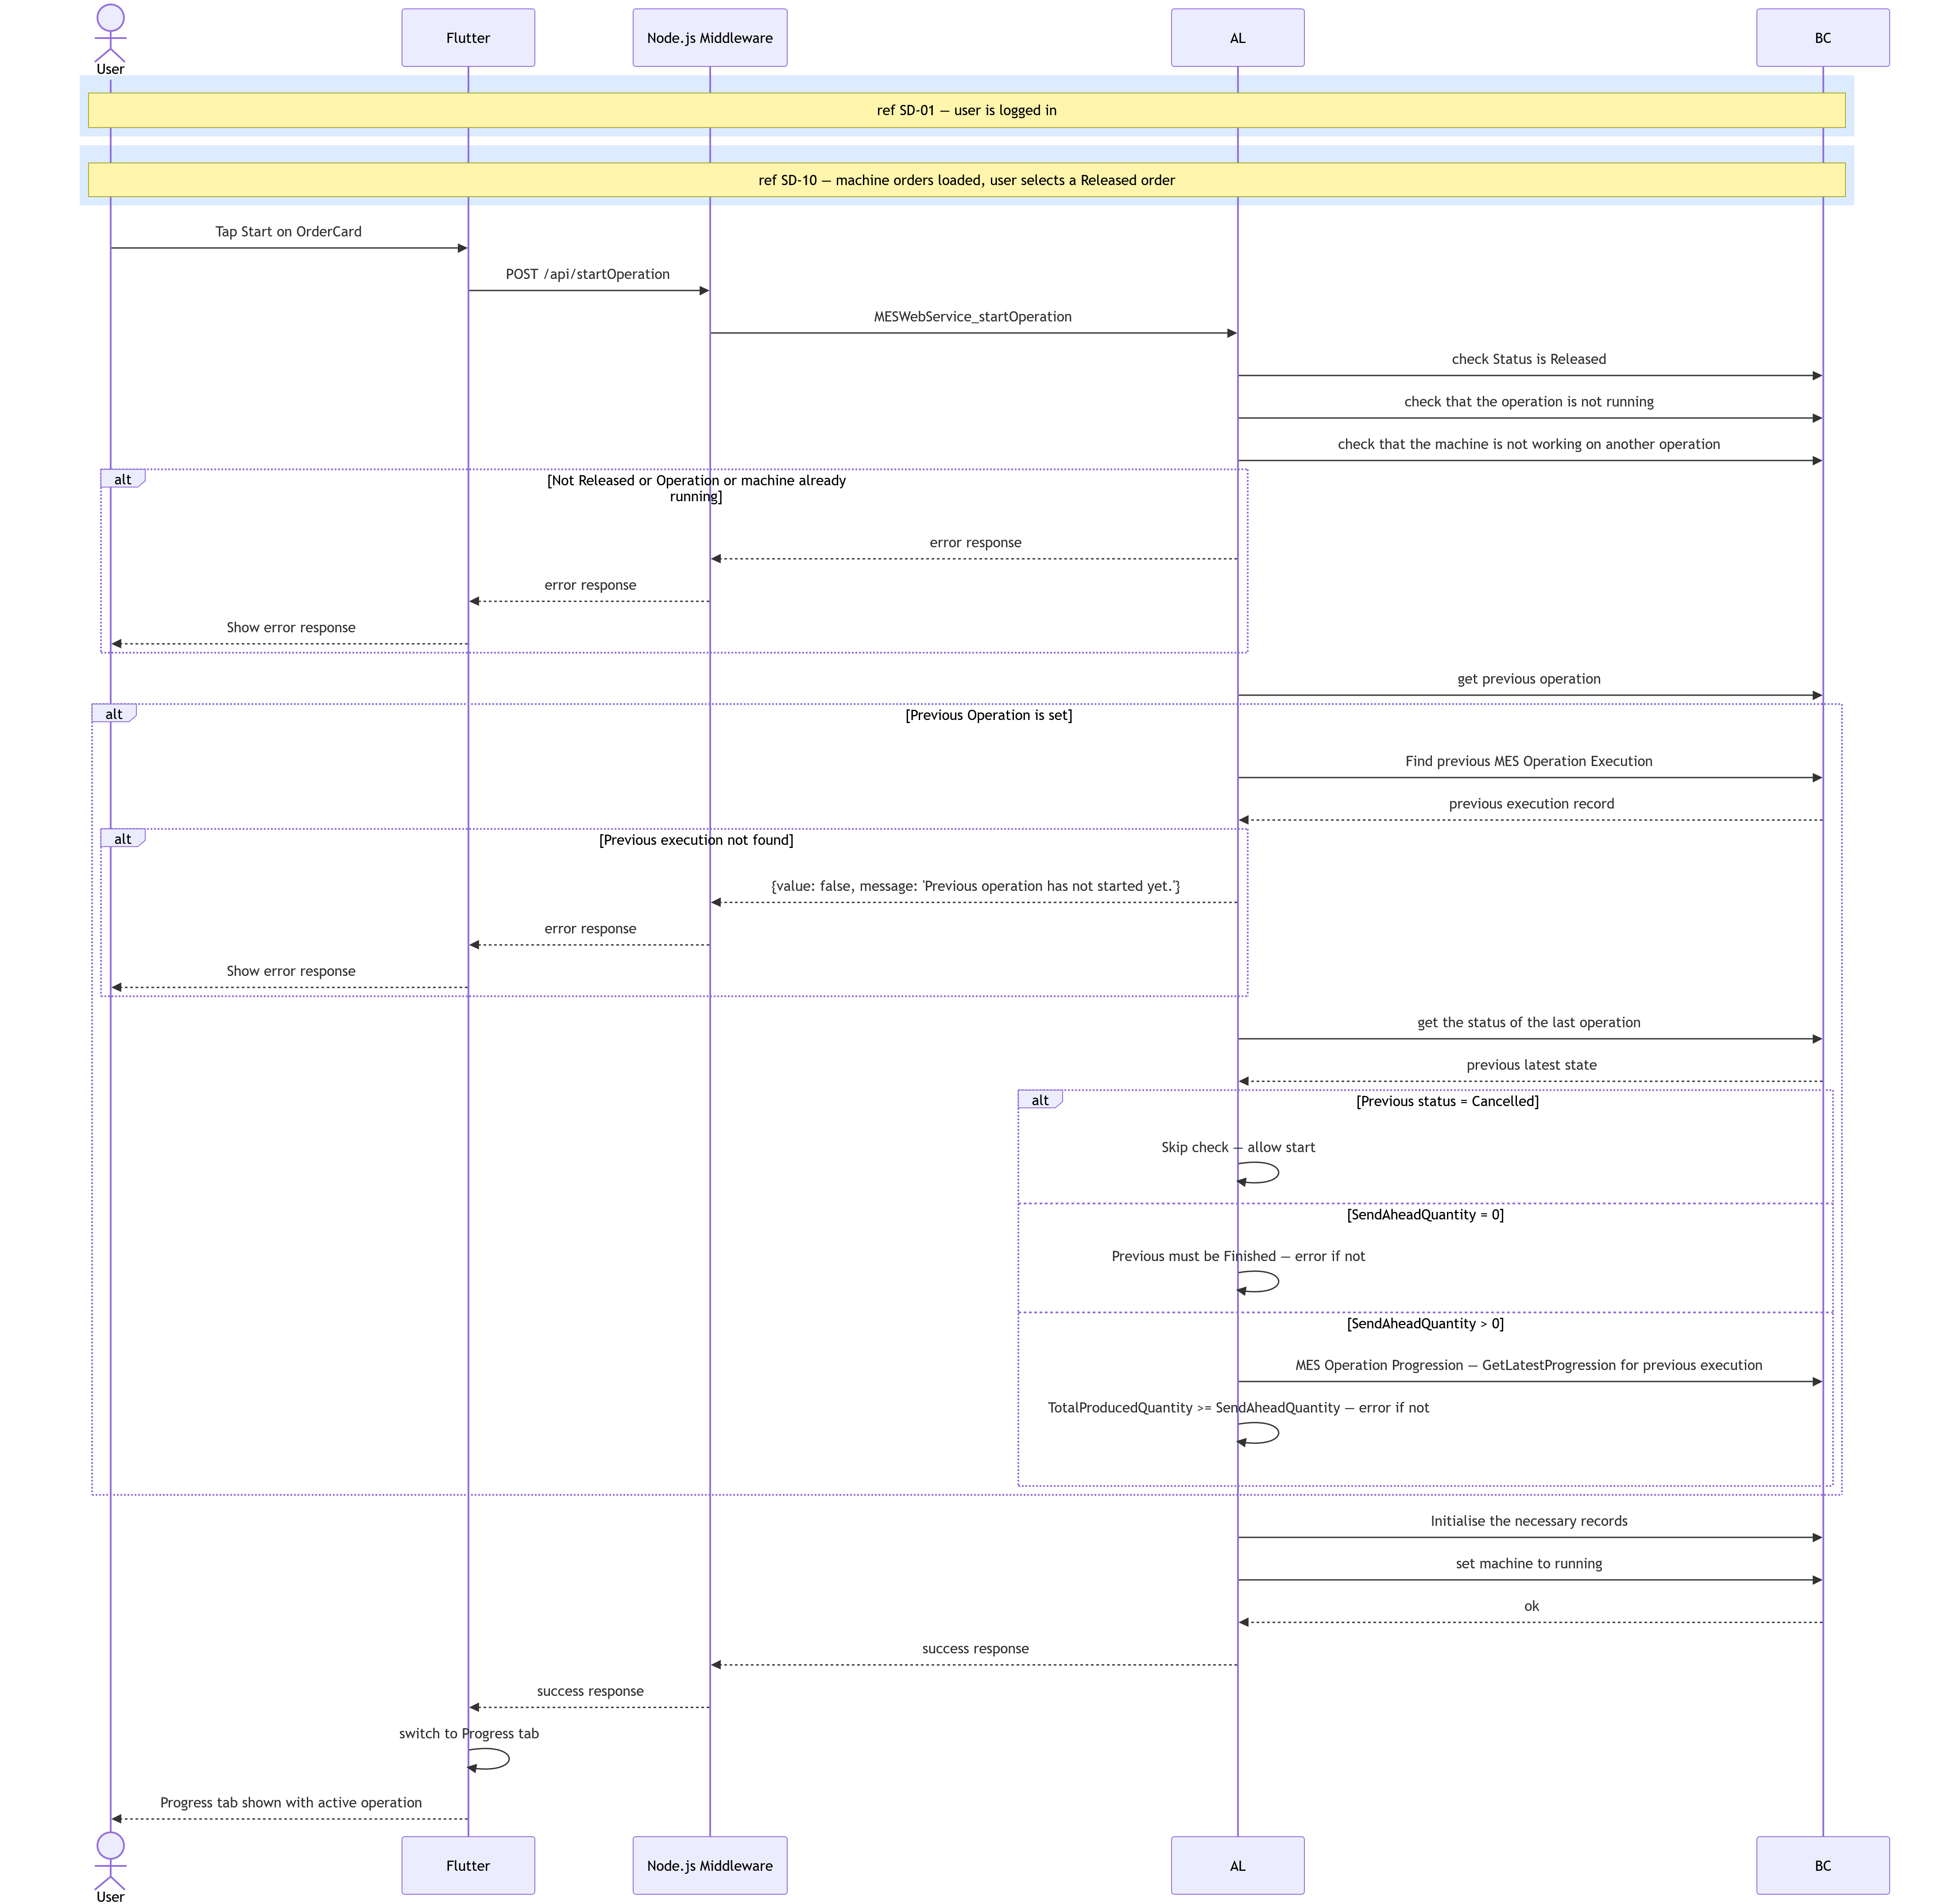
\includegraphics[width=\linewidth,height=0.82\textheight,keepaspectratio]{./media/MES_Sprint-2-Repport/diagrams/sequence/start-order.png}
  \caption{SD-11: Start Operation.}
  \label{fig:s2-seq-start-operation}
\end{figure}


%=====SD-11==========================================================
% sequenceDiagram
%     actor User
%     participant Flutter
%     participant AL
%     participant BC

%     rect rgb(220,235,255)
%         Note over User,BC: ref SD-01 — user is logged in and holds a valid token
%     end
%     rect rgb(220,235,255)
%         Note over User,BC: ref SD-10 — machine orders loaded user selects a Released order
%     end

%     User->>Flutter: Tap Start on OrderCard
%     Flutter->>AL: startOperation request

%     rect rgb(220,235,255)
%         Note over User,BC: ref SD-02 — AL validates token and resolves operatorId
%     end

%     AL->>BC: check the order is released
%     BC-->>AL: routing line
%     AL->>BC: Check that the Operation is not running
%     AL->>BC: Check that the machine is not working
%     BC-->>AL: clear
%     alt Not Released or already running
%         AL-->>Flutter: error message
%         Flutter-->>User: Show error snackbar
%     else Valid
%         AL->>BC: Insert MES Operation Execution
%         BC-->>AL: executionId
%         AL->>BC: Insert MES Operation State
%         AL->>BC: Insert MES Operation Progression
%         AL->>BC: set machine as working
%         AL->>BC: Insert MES User Execution Interaction
%         BC-->>AL: ok
%         AL-->>Flutter: request response
%         Flutter->>User: redirect to Progress tab
%     end
%====================================================================

\begin{figure}[H]
  \centering
  
\includegraphics[height=0.30\textheight,keepaspectratio]{./media/MES_Sprint-2-Repport/placeholder-image.png}
  \caption{Fetch Operation progress --- Sequence Diagram.}
  \label{fig:s2-seq-fetch-progress}
\end{figure}

\begin{figure}[H]
  \centering
  
\includegraphics[height=0.30\textheight,keepaspectratio]{./media/MES_Sprint-2-Repport/placeholder-image.png}
  \caption{Fetch Operation History --- Sequence Diagram.}
  \label{fig:s2-seq-fetch-history}
\end{figure}

Figure~\ref{fig:s2-seq-fetch-history} shows the history retrieval sequence. The
\techname{Flutter} frontend calls the same
\apiendpoint{fetchOperationsStatusAndProgress} endpoint used by the active
monitoring view, but with \texttt{fetchFinished = true}. The
\techname{Business Central} backend returns only executions whose latest status
record is \domainterm{Finished} or \domainterm{Cancelled}, along with resolved
start and end timestamps.

\subsection{Class Diagram}

The UML Class Diagram (Figure~\ref{fig:s2-class-diagram-s2}) of the machine and
production management domain shows the \modulename{MES Machine Status} and
\modulename{MES Operation Status} tables and their relationships with the
\techname{Business Central} standard tables \modulename{Machine Center} and
\modulename{Prod. Order Routing Line}.

\begin{figure}[H]
  \centering
  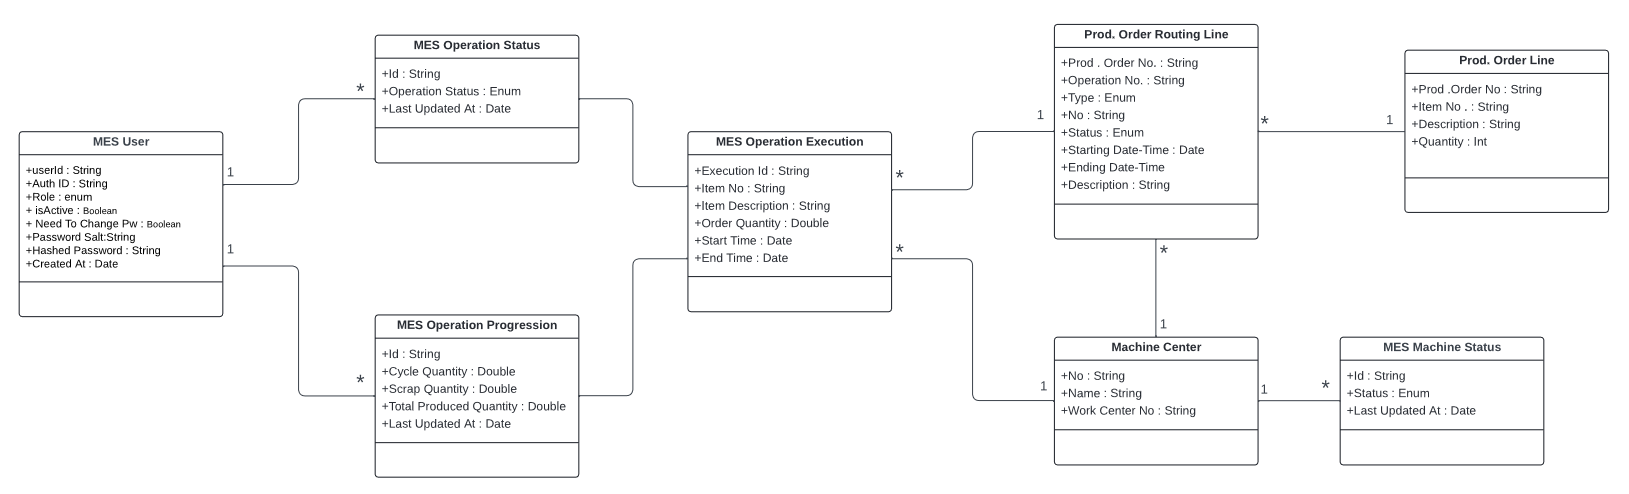
\includegraphics[width=\linewidth,height=0.82\textheight,keepaspectratio]{./media/MES_Sprint-2-Repport/diagrams/class/sprint2-diagram.png}
  \caption{UML Class Diagram --- Machine \& Production Management.}
  \label{fig:s2-class-diagram-s2}
\end{figure}

% ---------------------------------------------------------------------------
% 4. IMPLEMENTATION
% ---------------------------------------------------------------------------
\section{Implementation}

\subsection{Backend Implementation}

\subsubsection{Backend Structure Overview}

The machines domain follows the same layered structure established in Sprint~1.
Two new sub-folders were added under \modulename{src/1-Tables/machines/} and
\modulename{src/2-Enum/machines/}, and a new codeunit was placed under
\modulename{src/3-CodeUnit/machines/}. The OData web service is published through
the existing \modulename{WebServices.xml} mechanism under a new service name.

\subsubsection{MES Machine Status Table}

The \modulename{MES Machine Status} table (50107) stores the full history of
machine state changes as an append-only log. Each insert creates a new record;
the most recent record per machine represents the current state. Table~\ref{tab:s2-mes_machine_status_fields}
lists the fields and their descriptions.

\begin{longtable}{@{} P{0.21\linewidth} P{0.17\linewidth} P{0.57\linewidth} @{}}
  
  \caption{MES Machine Status (Table 50107) --- Field Dictionary}
  \label{tab:s2-mes_machine_status_fields}\\
  \toprule
  \textbf{Name}           & \textbf{Type}                      & \textbf{Description} \\
  \midrule
  \endfirsthead
  
  \toprule
  \textbf{Name}           & \textbf{Type}                      & \textbf{Description} \\
  \midrule
  \endhead
  
  \multicolumn{3}{r}{\small Continued on next page} \\
  \endfoot
  
  \bottomrule
  \endlastfoot
  
  Id                      & Code[50]                           &                      
  Primary key. GUID-derived value assigned automatically on insert if blank. \\
  \midrule
  
  Machine No.             & Code[20]                           &                      
  Foreign key to \texttt{Machine Center."No."}. Identifies the machine this status
  record belongs to. \\
  \midrule
  
  Status                  & Enum (\texttt{MES Machine Status}) &                      
  Current machine state: \domainterm{Idle}, \domainterm{Starting}, or
  \domainterm{OutOfOrder}. \\
  \midrule
  
  Current Prod. Order No. & Code[20]                           &                      
  Foreign key to \texttt{Prod. Order Routing Line."Prod. Order No."}. Records which
  production order the machine is currently executing, if any. \\
  \midrule
  
  Last Updated At         & DateTime                           &                      
  UTC timestamp set automatically on insert. Used to find the most recent status
  record for a given machine. \\
  
\end{longtable}

\subsubsection{MES Operation Status Table}

The \modulename{MES Operation Status} table (50108) implements the same
append-only pattern for operation lifecycle events. Every state transition
(start, pause, resume, finish) inserts a new record; queries always sort by
\modulename{Last Updated At} descending to obtain the current state.
Table~\ref{tab:s2-mes_operation_status_fields} provides the full field dictionary.

\begin{longtable}{@{} P{0.21\linewidth} P{0.17\linewidth} P{0.57\linewidth} @{}}
  
  \caption{MES Operation State (Table 50108) --- Field Dictionary}
  \label{tab:s2-mes_operation_status_fields}\\
  \toprule
  \textbf{Name}    & \textbf{Type}                        & \textbf{Description} \\
  \midrule
  \endfirsthead
  
  \toprule
  \textbf{Name}    & \textbf{Type}                        & \textbf{Description} \\
  \midrule
  \endhead
  
  \multicolumn{3}{r}{\small Continued on next page} \\
  \endfoot
  
  \bottomrule
  \endlastfoot
  
  Id               & Code[50]                             &                      
  Primary key. GUID-derived identifier assigned automatically on insert. \\
  \midrule
  
  Execution Id     & Code[50]                             &                      
  Foreign key to \texttt{MESOperationExecution}. \\
  \midrule
  
  
  
  Operator Id      & Code[50]                             &                      
  Foreign key to \texttt{MES User."User Id"}. The operator who triggered the
  state transition. \\
  \midrule
  
  Operation Status & Enum (\texttt{MES Operation Status}) &                      
  Lifecycle state at the time of this record: \domainterm{Running},
  \domainterm{Paused}, or \domainterm{Finished}. \\
  \midrule
  
  Last Updated At  & DateTime                             &                      
  UTC timestamp set automatically on insert. Together with the composite key
  (Machine No, Prod Order No, Operation No), this field is used to retrieve the
  current status via descending sort. \\
  
\end{longtable}

Key points:

\begin{itemize}
  \item Both tables use an append-only design: no \texttt{Modify} is called on
        existing records.
  \item The \domainterm{secondary index}
        \texttt{ExecutionTimeline("Execution Id", "Last Updated At")} on \modulename{MES Operation State} supports
        efficient retrieval of the latest event per group.
\end{itemize}

\subsubsection{Enumerations}

Two enumerations support the domain.
\modulename{MES Machine Status} (Enum 50101) defines three values:
\domainterm{Idle}, \domainterm{Starting}, and \domainterm{OutOfOrder}.
\modulename{MES Operation Status} (Enum 50102) defines three values:
\domainterm{Running}, \domainterm{Paused}, and \domainterm{Finished}.
Both enumerations are declared \texttt{Extensible = true} to allow future
additions without modifying the base objects.

\subsubsection{Machine Actions Business Logic}

All machine and operation business logic is encapsulated in codeunit 50130
\modulename{MES Machine Actions}. The codeunit exposes four public procedures
that are called directly by the OData web service layer.

\textbf{FetchMachines.}
Accepts a \domainterm{work centre number} and returns a \domainterm{JSON} array
of machine objects. For each \modulename{Machine Center} record scoped to the
given work centre, the procedure looks up the latest \modulename{MES Machine
  Status} record via \texttt{FindLast()} and inlines the current status and active
production order number into the response object. If no status record exists, the
machine is reported as \domainterm{Idle}.

\textbf{getMachineOrders.}
Accepts a machine number and returns a \domainterm{JSON} array of production
routing lines whose status is \domainterm{Planned}, \domainterm{Firm Planned}, or
\domainterm{Released} and whose type is \domainterm{Machine Center}. Routing
lines that already have an existing \modulename{MES Operation Status} record are
excluded from the result, ensuring that only work not yet started is shown in the
order list. For each qualifying line, the corresponding
\modulename{Prod. Order Line} is joined to supply item description and order
quantity.

\textbf{startOperation.}
Accepts a production order number, operation number, and machine number. The
procedure delegates precondition checking to a \texttt{[TryFunction]}
(\modulename{TryStartOperation}) that enforces \businessrule{BR-OPS-001}: it
verifies the routing line is \domainterm{Released}, confirms no \domainterm{Running}
record exists for the same order/operation, and checks that the machine is not
already busy with another operation. If all checks pass, a new
\modulename{MES Operation Status} record with status \domainterm{Running} is
inserted by \modulename{InsertMESOperation}. On failure, the last error text is
captured and returned as a structured \domainterm{JSON} error response.

\textbf{fetchMachineOperationStatus.}
Returns the current active operations for a machine as a \domainterm{JSON} array.
The procedure sets a descending composite key on
(Machine No, Prod Order No, Operation No, Last Updated At) and iterates the
result set, emitting at most one entry per (order, operation) pair --- the one
with the most recent timestamp. Only entries whose latest status is
\domainterm{Running} or \domainterm{Paused} are included in the output, satisfying
\businessrule{BR-OPS-003}.

\subsection{REST API and Web Services Implementation}

Communication between \techname{Flutter} and \techname{Business Central} for the
machines domain uses the same \domainterm{OData V4 Unbound Actions} pattern
established in Sprint~1. A new web service entry was added to
\modulename{WebServices.xml} exposing codeunit 50130 under the service name
\texttt{MESMachinesActionsEndpoints}. After deployment, the four procedures are
reachable at the following endpoints:

\begin{itemize}
  \item \apiendpoint{POST .../ODataV4/MESWebService\_FetchMachines}
  \item \apiendpoint{POST .../ODataV4/MESWebService\_getMachineOrders}
  \item \apiendpoint{POST .../ODataV4/MESWebService\_startOperation}
  \item \apiendpoint{POST .../ODataV4/MESWebService\_fetchMachineOperationStatus}
\end{itemize}

All endpoints follow the same \domainterm{JSON} request/response convention used
by the authentication layer: the request body carries named parameters as
top-level \domainterm{JSON} fields, and the response wraps the \techname{AL}
return value inside a \texttt{"value"} field which the \techname{Flutter} service
layer double-decodes.

\subsection{Frontend Implementation}

\noindent
\begin{minipage}[t]{0.6\textwidth}
  \vspace{0pt}
  The machines domain retains the same four-layer call stack introduced in
  Sprint~1 (\domainterm{Model} \textrightarrow{} \domainterm{Service}
  \textrightarrow{} \domainterm{Provider} \textrightarrow{} \domainterm{UI}), but
  Sprint~2 introduced a significant reorganisation of the \domainterm{UI layer}
  file structure, making the codebase easier to maintain and facilitating code
  reuse across components.
  
  \subsubsection{Model Layer}
  
  Two models were introduced.
  \modulename{MachineModel} (\modulename{mes\_machine\_model.dart}) holds the
  machine number, name, current status string, and active order number, populated
  from the \apiendpoint{FetchMachines} response.
  \modulename{MachineOrderModel} (\modulename{erp\_order\_model.dart}) holds the
  full set of production order fields returned by \apiendpoint{getMachineOrders},
  including order number, status, operation number, planned start and end
  \domainterm{DateTime} values, item number, item description, order quantity, and
  operation description.
  
  
  \subsubsection{Service Layer}
  
  Two service classes handle all network communication for the machines domain.
  \modulename{MESMachineListService} (\modulename{mes\_MachineList.dart}) exposes a
  \modulename{fetchMachines} method that posts the work centre number and parses the
  double-encoded \domainterm{JSON} array into a list of \modulename{MachineModel}
  objects. It also exposes a \modulename{streamMachines} method that wraps
  \modulename{fetchMachines} in an \texttt{async*} generator loop with a
\end{minipage}
\hfill
\begin{minipage}[t]{0.38\textwidth}
  \vspace{0pt}
  \centering
  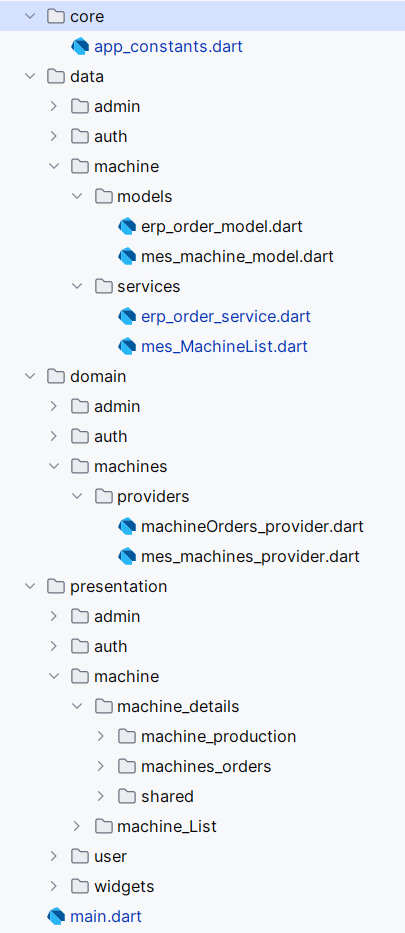
\includegraphics[width=\linewidth]{./media/MES_Sprint-2-Repport/screenshots/frontend-structure.png}
  \captionof{figure}{\techname{Flutter} machines domain --- layered architecture.}
  \label{fig:s2-flutter-architecture-s2}
\end{minipage}


5-second \texttt{Future.delayed} delay, emitting an updated list on every cycle and
yielding an empty list on error to prevent the \domainterm{StreamBuilder} from
entering an error state.


\modulename{ErpMachineOrdersService} (\modulename{erp\_order\_service.dart})
exposes three methods: \modulename{getMachineOrders} for fetching the order list,
\modulename{getStartOperationValidation} for triggering the start operation
endpoint and parsing the success/failure result, and
\modulename{fetchMachineOperationStatus} for retrieving active operation records.
A \modulename{streamMachines} generator on this service applies the same 5-second
polling pattern for the operations progress view.


\subsubsection{State Management Layer}

Two providers were introduced.
\modulename{MesMachinesProvider} (\modulename{mes\_machines\_provider.dart}) is a
plain (non-\texttt{ChangeNotifier}) provider that delegates directly to the
\modulename{MESMachineListService} stream. Because all state is carried by the
stream itself, no \texttt{notifyListeners} mechanism is needed and the
\domainterm{StreamBuilder} in the UI subscribes directly to the emitted values.

\modulename{MachineordersProvider} (\modulename{machineOrders\_provider.dart})
wraps both the order list fetching and the operation start flow with the standard
\texttt{ChangeNotifier} pattern. It exposes \modulename{getMachineOrders} which
populates a \modulename{machineOrders} list, and \modulename{startOrder} which
calls the service and returns a boolean success flag. It also exposes
\modulename{getMachineOperationsStatusStream} which passes the polling stream
through directly to the UI layer.

\subsubsection{User Interface}

The \uilabel{Machine List Page} is the entry point for operators after login. It
displays a live-updating grid (tablet/desktop) or list (mobile) of machine cards
scoped to the authenticated work centre. Each card shows the machine name, its
current status with a colour-coded badge, and the active production order number.
The layout adapts across breakpoints: a single-column list below 600 dp, a
two-column grid below 1024 dp, and a four-column grid above.
As illustrated in Figure~\ref{fig:s2-ui-machine-list}, the interface is consistent
across both desktop and mobile platforms.

\begin{figure}[H]
  \centering
  \setlength{\fboxsep}{5pt}
  \colorbox{black}{%
    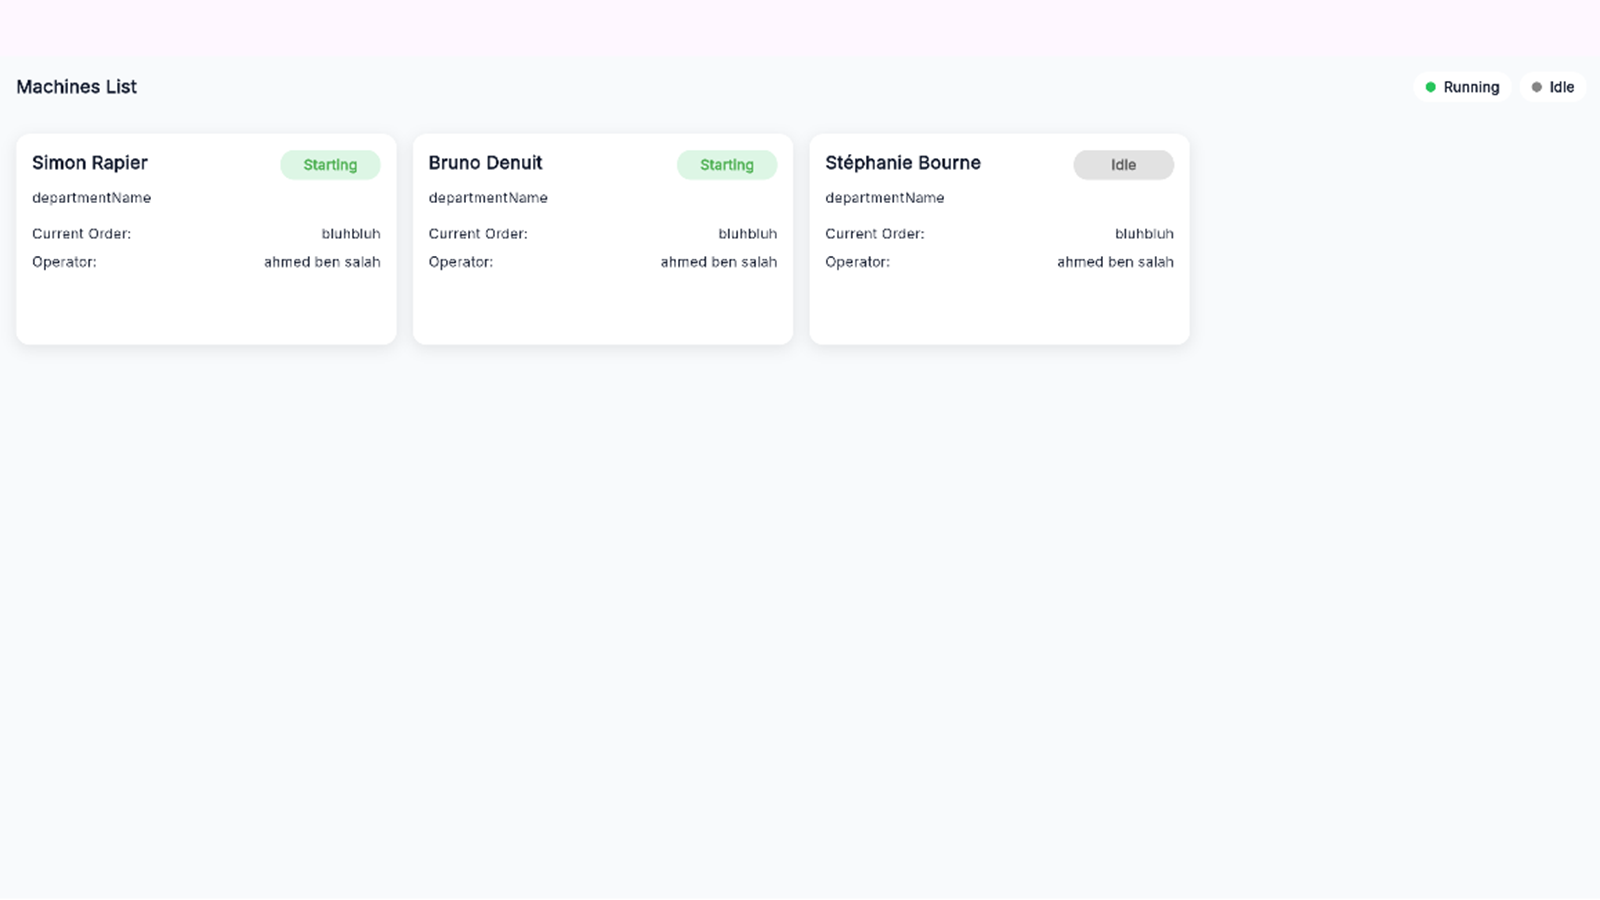
\includegraphics[height=0.3\textheight,keepaspectratio]{./media/MES_Sprint-2-Repport/UI/desktop-machines.png}%
    \hspace{\fboxsep}%
    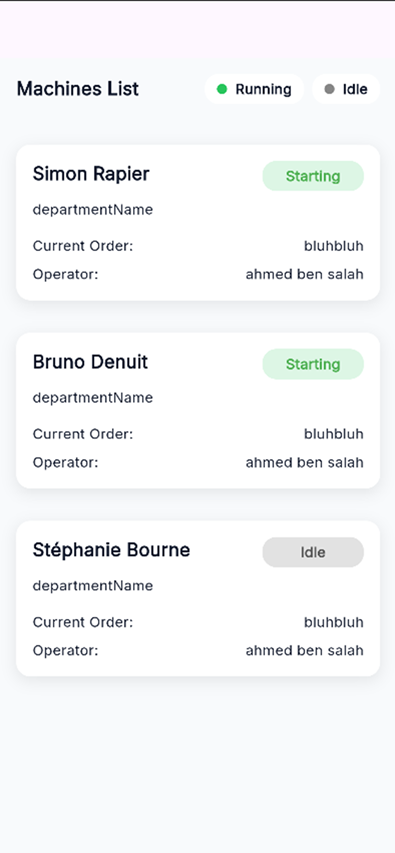
\includegraphics[height=0.3\textheight,keepaspectratio]{./media/MES_Sprint-2-Repport/UI/mobile-machines.png}%
  }
  \caption{\uilabel{Machine List Page} --- desktop and mobile views.}
  \label{fig:s2-ui-machine-list}
\end{figure}

The user interface for the machines domain is split across two top-level pages
accessible via a shared \uilabel{Top Navigation Bar} with tabs for
\uilabel{Orders}, \uilabel{Progress}, \uilabel{Consumable}, and \uilabel{History}.

The \uilabel{Machine Orders Page} displays the production routing lines assigned to the selected machine. A \uilabel{Global Search Bar} allows filtering by free text (order number, item description, or date), by status, and sorting by planned start date. Order cards use a responsive layout that switches between a stacked \domainterm{narrow layout} and a side-by-side \domainterm{wide layout} at a 520 dp breakpoint. Only \domainterm{Released} orders display an active \uilabel{Start Order} button; \domainterm{Planned} and \domainterm{Firm Planned} orders show it disabled. Figure~\ref{fig:s2-ui-machine-orders} illustrates both the desktop and mobile views.

\begin{figure}[H]
  \centering
  \setlength{\fboxsep}{5pt}
  \colorbox{black}{%
    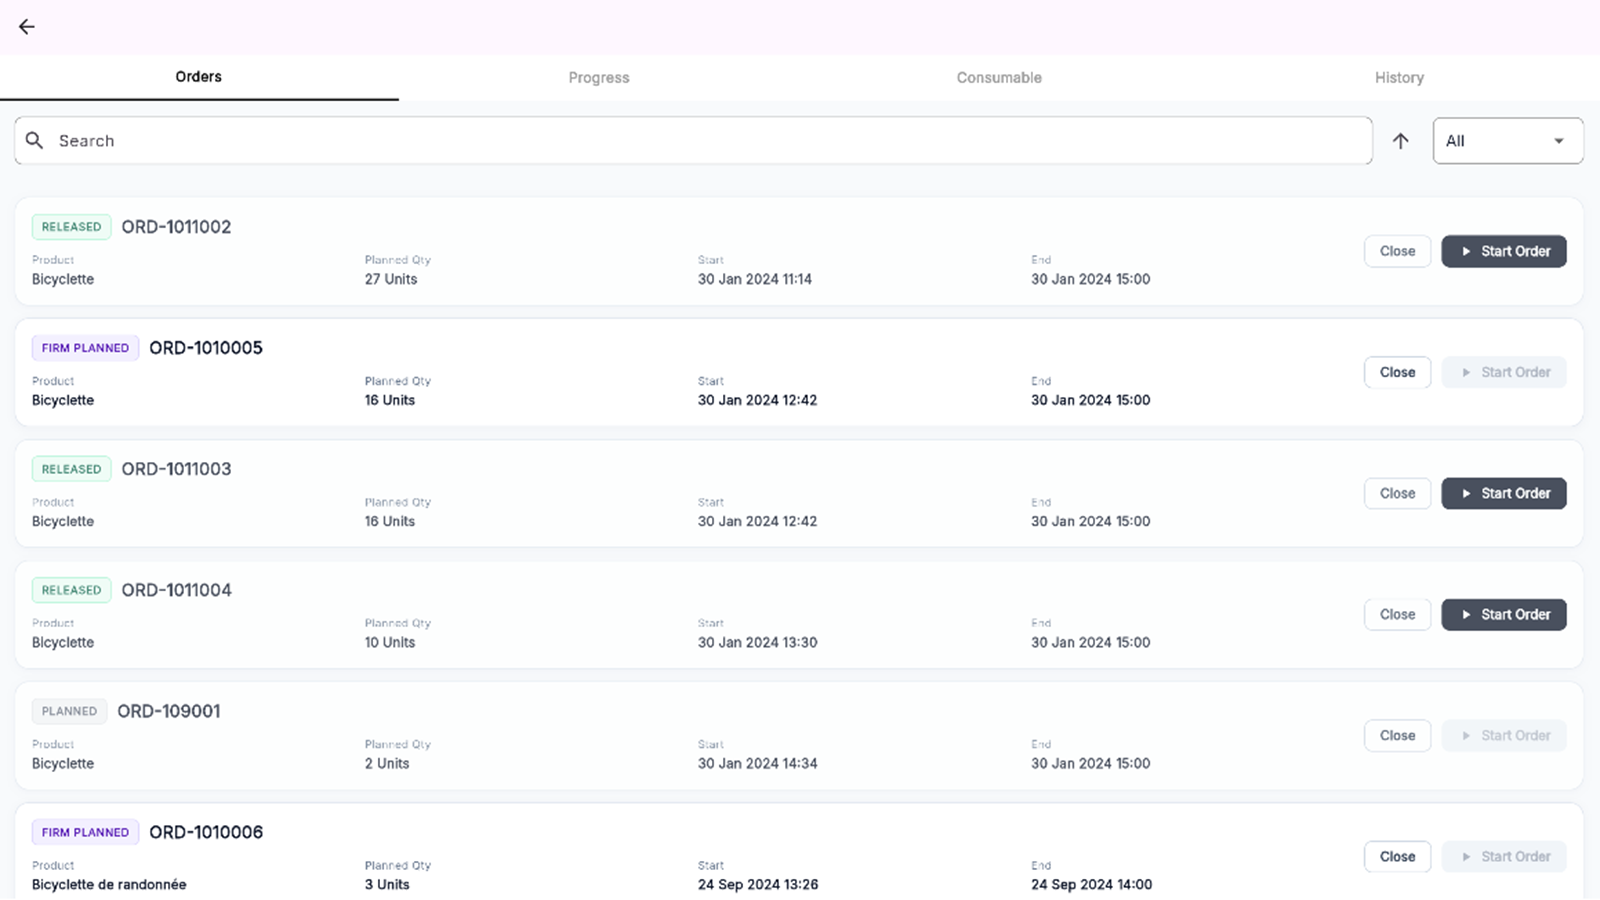
\includegraphics[height=0.3\textheight,keepaspectratio]{./media/MES_Sprint-2-Repport/UI/dektop-waiting_orders.png}%
    \hspace{\fboxsep}%
    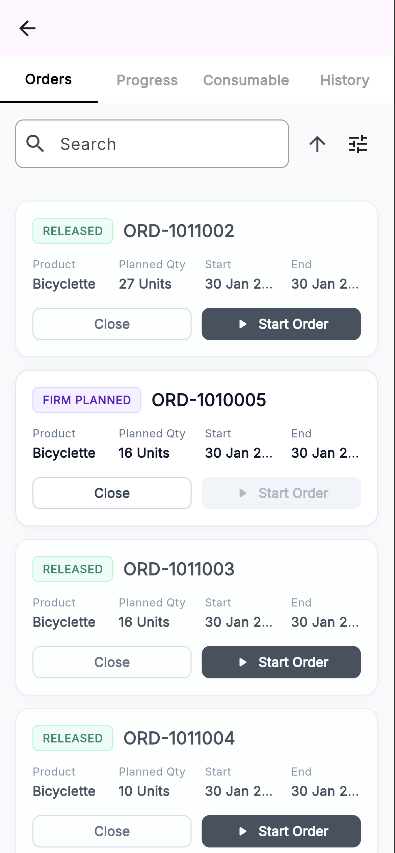
\includegraphics[height=0.3\textheight,keepaspectratio]{./media/MES_Sprint-2-Repport/UI/mobile-waiting_orders.png}%
  }
  \caption{\uilabel{Machine Orders Page} --- desktop and mobile views.}
  \label{fig:s2-ui-machine-orders}
\end{figure}

The \uilabel{Orders Progression Page} displays the currently active operations on
a machine, polling every 5 seconds. Each
operation card shows a colour-coded status badge (green for \domainterm{Running},
amber for \domainterm{Paused}), the order and operation identifiers, the last
updated timestamp, and a progress bar. The card layout also switches between narrow and wide
variants at the 520 dp breakpoint. \uilabel{Pause} and \uilabel{Resume} action
buttons adapt their colour and label to the current operation status, as shown in
Figure~\ref{fig:s2-ui-operations-progress}.

\begin{figure}[H]
  \centering
  \setlength{\fboxsep}{5pt}
  \colorbox{black}{%
    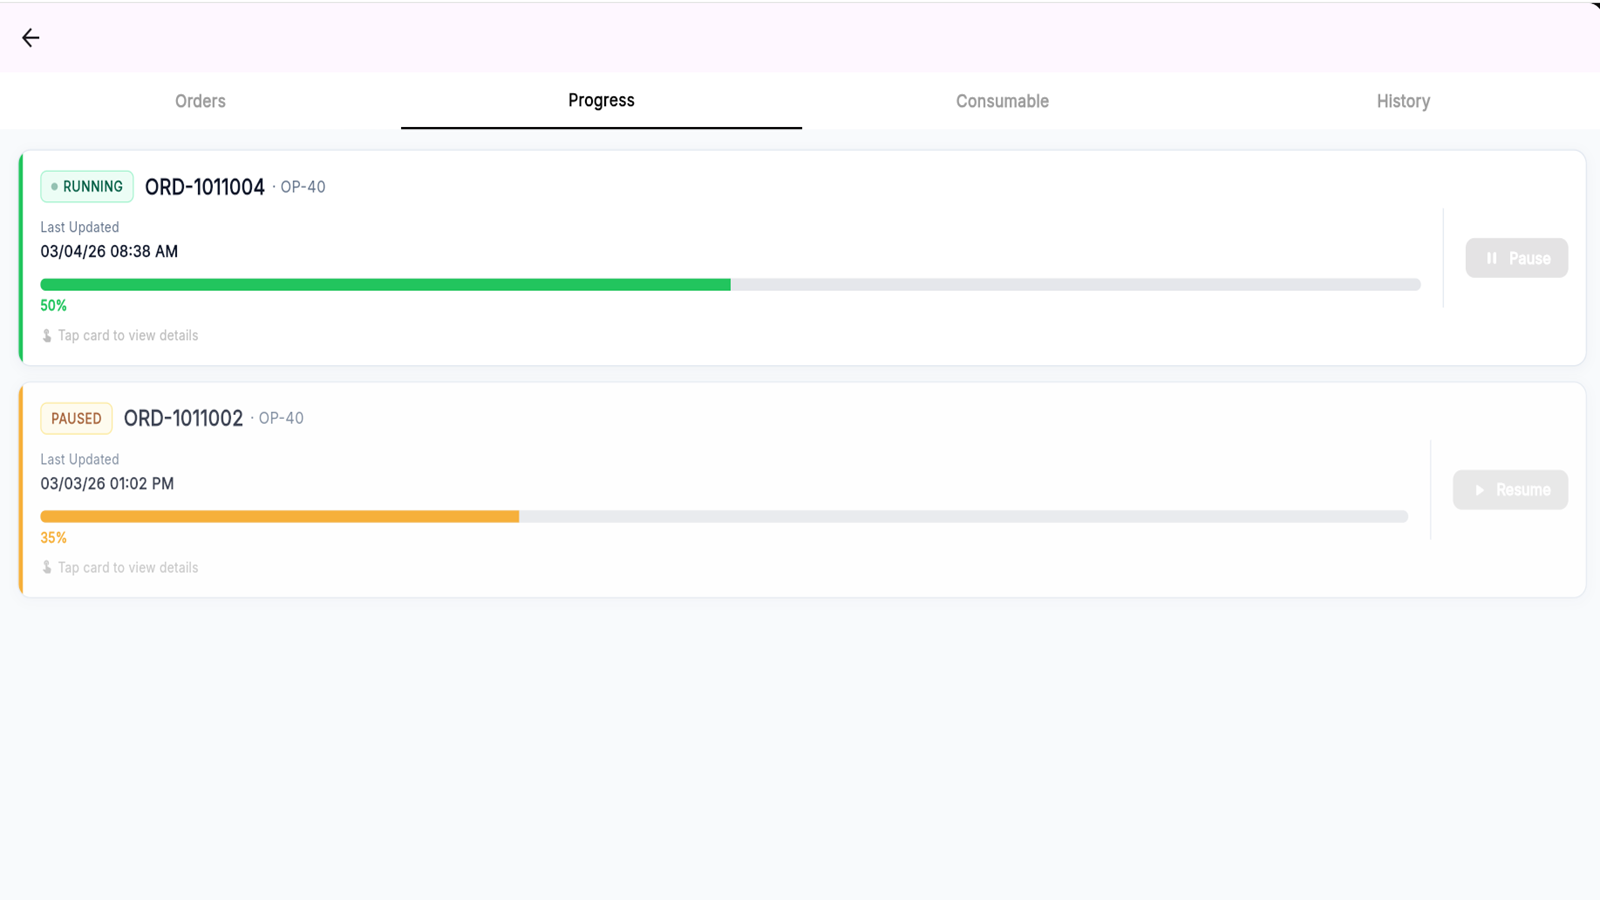
\includegraphics[height=0.3\textheight,keepaspectratio]{./media/MES_Sprint-2-Repport/UI/desktop-order_progress.png}%
    \hspace{\fboxsep}%
    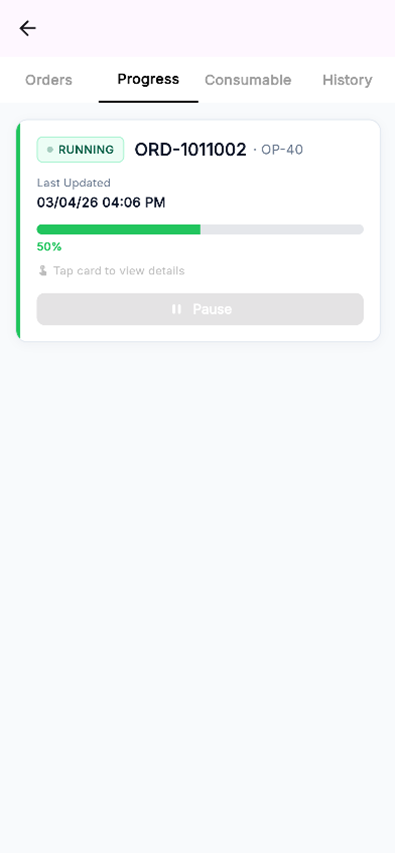
\includegraphics[height=0.3\textheight,keepaspectratio]{./media/MES_Sprint-2-Repport/UI/mobile-order_progress.png}%
  }
  \caption{\uilabel{Orders Progression Page} --- desktop and mobile views.}
  \label{fig:s2-ui-operations-progress}
\end{figure}

The \uilabel{Machine History Page} (Figure~\ref{fig:s2-ui-hist-page}) displays completed operations assigned to the selected machine, limited to \domainterm{Finished} and \domainterm{Cancelled} statuses. It shares the same layout and filtering behaviour as the \uilabel{Machine Orders Page} --- including free-text search, status filtering, and sort controls --- but omits the \uilabel{Start Order} button. Tapping an operation card navigates to its \uilabel{Operation Detail Page} for review. The \uilabel{Machine History Page} is accessible via the \domainterm{History} tab in the \techname{TopNavigationBar}. Figure~\ref{fig:s2-ui-hist-page} shows the desktop and mobile views.

\begin{figure}[H]
  \centering
  \setlength{\fboxsep}{5pt}
  \colorbox{black}{%
    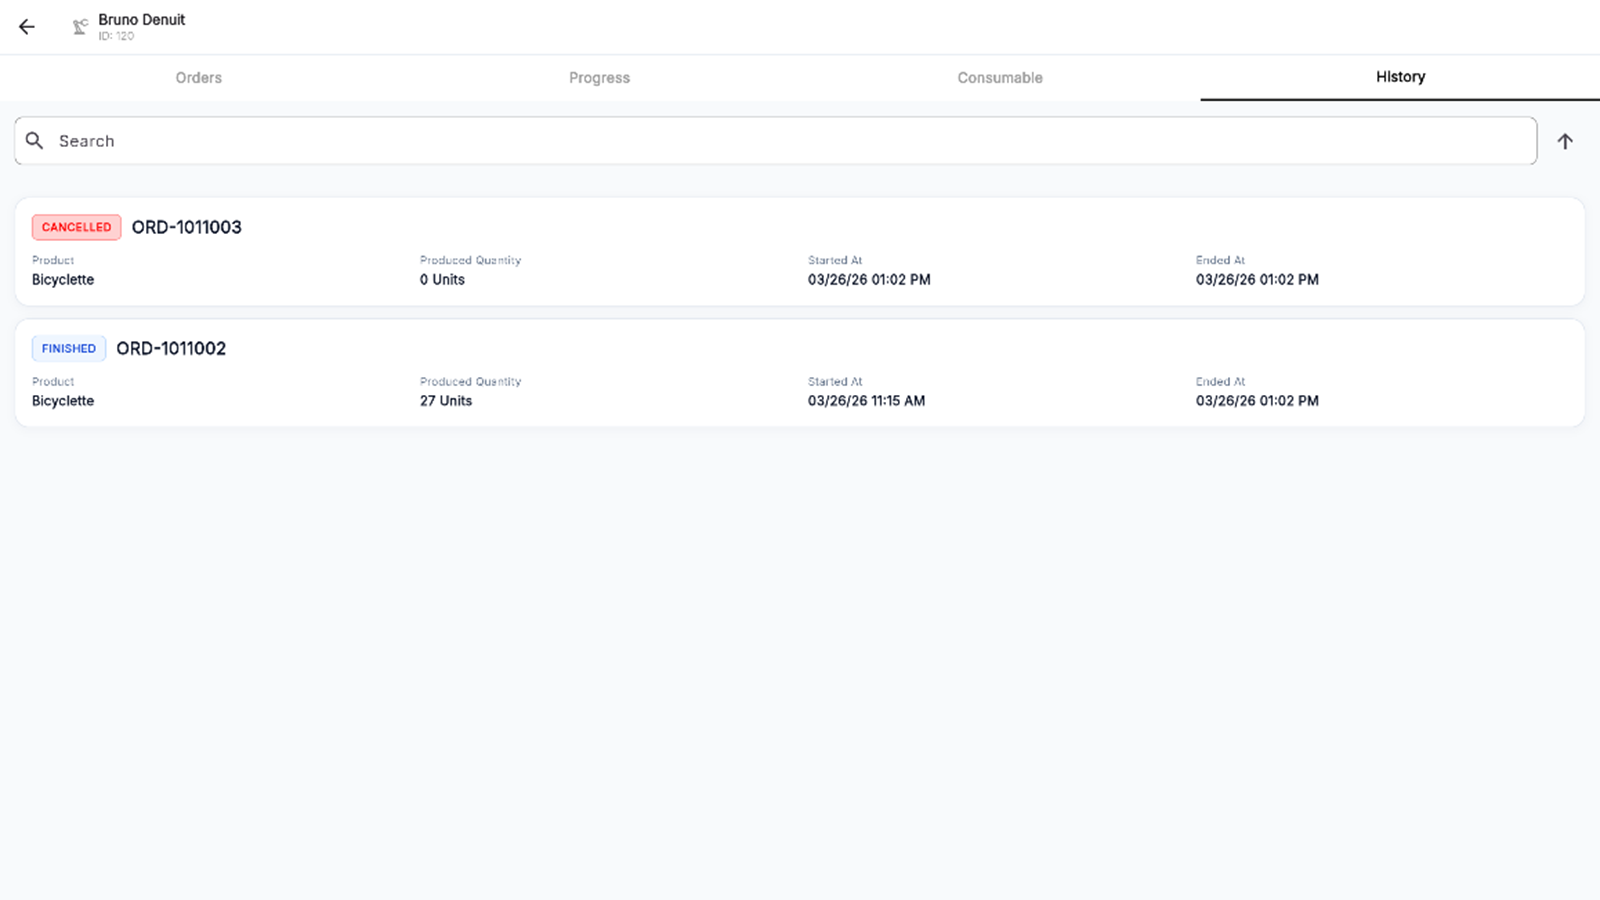
\includegraphics[height=0.3\textheight,keepaspectratio]{./media/MES_Sprint-2-Repport/UI/desktop-histPage.png}%
    \hspace{\fboxsep}%
    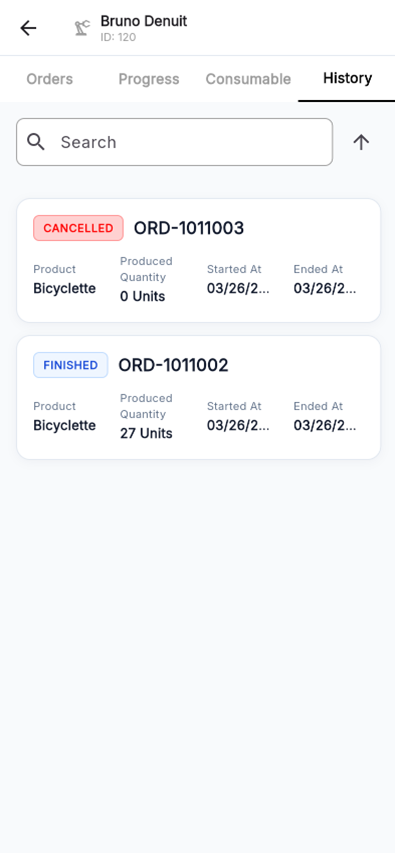
\includegraphics[height=0.3\textheight,keepaspectratio]{./media/MES_Sprint-2-Repport/UI/mobile-histPage.png}%
  }
  \caption{\uilabel{Machine History Page} --- desktop and mobile views.}
  \label{fig:s2-ui-hist-page}
\end{figure}


% ---------------------------------------------------------------------------
% CONCLUSION
% ---------------------------------------------------------------------------
\phantomsection
\section*{Conclusion}
\addcontentsline{toc}{section}{Conclusion}

This sprint successfully delivered the machine monitoring and production order
management foundation of the \domainterm{MES} application. On the backend, two
new append-only tables (\modulename{MES Machine Status} and
\modulename{MES Operation Status}) and a dedicated codeunit
(\modulename{MES Machine Actions}) were implemented in \techname{Business Central
  AL}, exposing four \domainterm{OData V4} endpoints that cover the full machine and
operation lifecycle. The append-only design ensures a complete, tamper-evident
audit trail of every state transition without requiring any record modification.

All business rules defined at the start of the sprint have been enforced: work
centre scoping (\businessrule{BR-MCH-002}), start operation validation
(\businessrule{BR-OPS-001}), immutable history (\businessrule{BR-OPS-002}),
active operation querying (\businessrule{BR-OPS-003}), and history scope
(\businessrule{BR-HIST-001}). The \techname{Flutter} frontend delivers a
responsive, real-time interface with 5-second polling streams for the machine
list and operations progress view, and a one-shot history load for the completed
operation audit log. The codebase is now ready to extend in Sprint~3 with
consumable tracking, operation finishing, and production declaration.


% ---------------------------------------------------------------------------
% Sprint 3 Production Execution \& Traceability
% ---------------------------------------------------------------------------
\chapter{Sprint 3 Production Execution \& Traceability}
\graphicspath{{./media/MES_Sprint-3-Repport/}}
\minitoc
\newpage
\section*{Introduction}
\addcontentsline{toc}{section}{Introduction}

This sprint report covers \textbf{Domain 3: Production Execution \& Traceability}.
Building upon the authentication and machine monitoring infrastructure established
in the previous sprints, this sprint delivers the core production execution
features; declaring production output, pausing and resuming operations, finishing, Interrupting 
or cancelling orders, tracking production declarations over time, monitoring Bill of
Materials consumption, component barcode scanning, scrap declaration, supervisor
proxy declaration, and label printing. The result is a fully operational shop-floor
execution loop from order assignment through to order closure, material traceability,
and printed part identification.

% ---------------------------------------------------------------------------
% 1. SPRINT BACKLOG
% ---------------------------------------------------------------------------
\section{Sprint Backlog}

This sprint covers \textbf{Domain 3:} \textbf{\domainterm{Production Execution \& Traceability}}.

% ----------------------------------------------------------
% US-3.1
% ----------------------------------------------------------
\begin{longtable}{@{} P{0.09\linewidth} P{0.38\linewidth} P{0.49\linewidth} @{}}
	\caption{US-3.1 --- Declare Production}
	\label{tab:s3-US-3.1} \\
	\toprule
	\textbf{ID} & \textbf{User Story} & \textbf{Tasks} \\
	\midrule
	\endfirsthead
	\toprule
	\textbf{ID} & \textbf{User Story} & \textbf{Tasks} \\
	\midrule
	\endhead
	\multicolumn{3}{r}{\small Continued on next page} \\
	\endfoot
	\bottomrule
	\endlastfoot
	
	\textbf{US-3.1}
	& As an \userrole{Operator} or \userrole{Supervisor}, I need to declare the
	produced quantity in a cycle so that the system records my
	production progress.
	& \noindent\textit{Business Central (AL):}
	\begin{itemize}[noitemsep, topsep=0pt, partopsep=0pt, leftmargin=*]
		\item Create table \techname{MES Operation Progression}.
		\item Create the functions:
		\begin{itemize}[noitemsep, topsep=0pt, partopsep=0pt, leftmargin=*]
			\item \texttt{TryDeclareProduction()} in codeunit \techname{MESMachineValidation}.
			\item \texttt{InsertNewProgressionCycle()} in codeunit \techname{MESMachineInsert}.
			\item \texttt{declareProduction()} in codeunit \techname{MESMachineWrite}.
		\end{itemize} 
		\item Expose \texttt{declareProduction()} through the codeunit \techname{MES Web Service}.
		\item Create page \techname{MES Operation Progression} list page.
	\end{itemize}
	\\ & &
	\noindent\textit{Flutter:}
	\begin{itemize}[noitemsep, topsep=0pt, partopsep=0pt, leftmargin=*]
		\item Updated \techname{ErpMachineOrdersService} to consume the \texttt{declareProduction} API and \techname{MachineordersProvider} to manage it.
	\end{itemize}
	\\ & &
	\noindent\textit{Flutter(continuation):}
	\begin{itemize}[noitemsep, topsep=0pt, partopsep=0pt, leftmargin=*]
		\item Create widget \techname{DeclareProductionDialog}.
		\item Add the \texttt{Declare Production} action in \techname{ActionButtonsContainer}.
	\end{itemize}\\
	\midrule
	\textbf{US-3.2}
	& As an \userrole{Operator} or \userrole{Supervisor}, I need to pause and
	resume an active operation so that production interruptions are tracked
	accurately.
	& \noindent\textit{Business Central (AL):}
	\begin{itemize}[noitemsep, topsep=0pt, partopsep=0pt, leftmargin=*]
		\item Create the functions:
		\begin{itemize}[noitemsep, topsep=0pt, partopsep=0pt, leftmargin=*] 
			\item \texttt{TryPauseOperation()} and \texttt{TryResumeOperation()} in codeunit \techname{MESMachineValidation}.
			\item \texttt{ExecuteOperationTransition()}, \texttt{pauseOperation()}, and \texttt{resumeOperation()} in codeunit \techname{MESMachineWrite}. 
		\end{itemize}
		\item Expose \texttt{pauseOperation()} and \texttt{resumeOperation()} throught codeunit \techname{MES Web Service}.
	\end{itemize}
	\\ & &
	\noindent\textit{Flutter:}
	\begin{itemize}[noitemsep, topsep=0pt, partopsep=0pt, leftmargin=*]
		\item Implement \techname{ErpMachineOrdersService} to consume the new endpoints 
		\item Implement \techname{MachineordersProvider} to manage its state.
		\item Create widget \techname{OperationActionButtons}.
		\item Implement pause/resume operation toggle handling in \techname{OrdersProgressionPage}.
	\end{itemize} \\
	\midrule
	\textbf{US-3.3}
	& As a \userrole{Supervisor}, I need to finish, interrupt or cancel a production
	operation so that the machine is released and the order is closed in the
	system.
	& \noindent\textit{Business Central (AL):}
	\begin{itemize}[noitemsep, topsep=0pt, partopsep=0pt, leftmargin=*]
		\item Create the functions:
		\begin{itemize}[noitemsep, topsep=0pt, partopsep=0pt, leftmargin=*]
			\item \texttt{TryCloseOperation()} in codeunit \techname{MESMachineValidation}.
			\item \texttt{InsertOperationStatus()}, \texttt{SetErpOrderToFinish()}, \texttt{InsertStartMESMachineStatus()}  and \texttt{InsertIdleMachineStatus()} in codeunit \techname{MESMachineInsert}.
			\item \texttt{finishOperation()} and \texttt{cancelOperation()} in codeunit \techname{MESMachineWrite}.
			\item \texttt{ExecuteCancelUnstartedOperation()} in codeunit \techname{MESMachineWrite}.
		\end{itemize}
		\item Expose \texttt{finishOperation()} and \texttt{cancelOperation()} in codeunit \techname{MES Web Service}.
	\end{itemize}
\\ & &
	\noindent\textit{Flutter:}
	\begin{itemize}[noitemsep, topsep=0pt, partopsep=0pt, leftmargin=*]
		\item Update \techname{ErpMachineOrdersService} to consume the new endpoints.
		\item Update \techname{MachineOrdersProvider} to manage its state.
		\item Update \techname{ActionButtonsContainer} to handle Finish/Interrupt operation flow.
	\end{itemize} \\
	\midrule
	\textbf{US-3.4}
	& As an \userrole{Operator} or \userrole{Supervisor}, I need a dedicated
	detail page for an operation so that I can see all real-time information
	in one place.
	& \noindent\textit{Business Central (AL):}
	\begin{itemize}[noitemsep, topsep=0pt, partopsep=0pt, leftmargin=*]
		\item Create table \techname{MES Operation Execution}.
		\item Create function \texttt{InsertMESOperationExecution()} in codeunit \techname{MESMachineInsert}.
		\item Create function \texttt{fetchOperationLiveData()} in codeunit \techname{MESMachineFetch}.
		\item Expose \texttt{fetchOperationLiveData()} through codeunit \techname{MES Web Service}.
		\item Create page \techname{MES Operation Execution}.
	\end{itemize}
\\ & &
	\noindent\textit{Flutter:}
	\begin{itemize}[noitemsep, topsep=0pt, partopsep=0pt, leftmargin=*]
		\item Create model \techname{OperationStatusAndProgressModel}.
		\item Update \techname{ErpMachineOrdersService} to consume the new endpoints.
		\item Update \techname{MachineOrdersProvider} to manage its state.
		\item Create page \techname{OperationDetailPage}.
		\item Create widget \techname{OperationAppBar}.
		\item Create widget \techname{CurrentOrderInfoContainer}.
	\end{itemize}\\
	\midrule
	
	\textbf{US-3.5}
	& As an \userrole{Operator} or \userrole{Supervisor}, I need to see all
	production cycles declared for an operation so that I can review each
	declaration's quantity, operator, and timestamp.
	& \noindent\textit{Business Central (AL):}
	\begin{itemize}[noitemsep, topsep=0pt, partopsep=0pt, leftmargin=*]
		\item Create function \texttt{fetchProductionCycles()} in codeunit \techname{MESMachineFetch}.
		\item Expose \texttt{fetchProductionCycles()} throught codeunit \techname{MES Web Service}.
	\end{itemize}
\\ & &
	\noindent\textit{Flutter:}
	\begin{itemize}[noitemsep, topsep=0pt, partopsep=0pt, leftmargin=*]
		\item Create model \techname{ProductionCycleModel}.
		\item Update \techname{ErpMachineOrdersService} to consume the new endpoints.
		\item Update \techname{MachineOrdersProvider} to manage its state.
		\item Create widget \techname{ProductionCycle}.
	\end{itemize} \\
\midrule
	
	\textbf{US-3.6}
	& As an \userrole{Operator} or \userrole{Supervisor}, I need to see a visual
	chart of production declarations over time so that I can identify trends
	and performance patterns.
	& \noindent\textit{Flutter:}
	\begin{itemize}[noitemsep, topsep=0pt, partopsep=0pt, leftmargin=*]
		\item Create widget \techname{ProductionChart}.
		\item create a function to ensure that the chart is always centered
		\item implemented a scrollable view into the chart
	\end{itemize}\\
	\midrule
	\textbf{US-3.7}
	& As an \userrole{Operator} or \userrole{Supervisor}, I need to see the
	Bill of Materials for a production operation so that I know which
	components are required, how much has already been consumed, and the amount 
	available in the inventory.
	& \noindent\textit{Business Central (AL):}
	\begin{itemize}[noitemsep, topsep=0pt, partopsep=0pt, leftmargin=*]
		\item Create function \texttt{fetchBom()} in codeunit \techname{MESMachineFetch}.
		\item Expose \texttt{fetchBom()} through codeunit \techname{MES Web Service}.
		
	\end{itemize}
\\ & &
	\noindent\textit{Flutter:}
	\begin{itemize}[noitemsep, topsep=0pt, partopsep=0pt, leftmargin=*]
		\item Create \techname{MesComponentConsumptionService} to consume the \texttt{fetchBom()} API.
		\item Create \techname{MesComponentConsumptionProvider} to manage BOM stream and refresh state.
		\item Create widget \techname{RequiredComponent}.
		\item Implement BOM streaming and refresh flow in \techname{MesComponentConsumptionService} and \techname{MesComponentConsumptionProvider}.
		\item Implement component status display and operation-based filtering in \techname{RequiredComponent} widget.
	\end{itemize}\\
	\midrule
	\textbf{US-3.8}
	& As an \userrole{Operator} or \userrole{Supervisor}, I need to report
	scrapped units with a reason code so that waste is accurately tracked.
	& \noindent\textit{Business Central (AL):}
	\begin{itemize}[noitemsep, topsep=0pt, partopsep=0pt, leftmargin=*]
		\item Create table \techname{MES Operation Scrap}.
		\item Create function \texttt{declareScrap()} in codeunit \techname{MES Machine Write}.
		\item Expose \texttt{declareScrap()} through codeunit \techname{MES Web Service}.
		\item Create \techname{MES Scrap Code API} to fetch scrap codes from the standard \techname{Business Central} \modulename{Scrap Code}.
	\end{itemize}
\\ & &
	\noindent\textit{Flutter:}
	\begin{itemize}[noitemsep, topsep=0pt, partopsep=0pt, leftmargin=*]
		\item Create model \techname{MesScrapCode}.
		\item Create \techname{MesScrapService} to consume the scrap code fetch and \texttt{declareScrap()} APIs.
		\item Create \techname{MesScrapProvider} to manage scrap code and scrap declaration state.
		\item Create dialog \techname{DeclareScrapDialog}.
	\end{itemize}\\
	\midrule
	\textbf{US-3.9}
	& As a \userrole{Supervisor}, I need to declare production on behalf of an
	operator so that output is attributed to the correct person.
	& \noindent\textit{Business Central (AL):}
	\begin{itemize}[noitemsep, topsep=0pt, partopsep=0pt, leftmargin=*]
		\item Add field \texttt{Declared By} to the tables \techname{MES Operation Progression} and \techname{MES Operation Scan}.
	\end{itemize}
\\ & &
	\noindent\textit{Flutter:}
	\begin{itemize}[noitemsep, topsep=0pt, partopsep=0pt, leftmargin=*]
		\item Create widget \techname{OperatorSelector}.
		\item Update \techname{DeclareProductionDialog} to support supervisor declaration on behalf of an operator.
		\item Connect \techname{OperatorSelector} to \techname{MesUserProvider} and pass \texttt{onBehalfOfUserId} to \techname{MachineOrdersProvider.declareProduction()}.
	\end{itemize} \\
	\midrule
	\textbf{US-3.10}
	& As an \userrole{Operator} or \userrole{Supervisor}, I need to scan
	components into an operation so that consumption is recorded against the BOM.
	& \noindent\textit{Business Central (AL):}
	\begin{itemize}[noitemsep, topsep=0pt, partopsep=0pt, leftmargin=*]
		\item Create table \techname{MES Component Scan}.
		\item Create the function \texttt{insertScans()} in codeunit \techname{MES Machine Write}.
		\item Create the functions  \texttt{resolveBarcode()} in codeunit \techname{MES Machine Fetch}.
		\item Expose the three function through codeunit \techname{MES Web Service}.
		\item Create page \techname{MES Component Consumption}.
	\end{itemize}
\\ & &
	\noindent\textit{Flutter:}
	\begin{itemize}[noitemsep, topsep=0pt, partopsep=0pt, leftmargin=*]
		\item Create model \techname{ItemBarcodeModel}.
		\item Create \techname{MesBarcodeService} to consume the endpoints \texttt{insertScans()}, and \texttt{resolveBarcode()}.
		\item Create \techname{MesBarcodeProvider} to manage barcode state and API calls.
		\item Create widget \techname{ScannerWidget}.
		\item Update widget \techname{RequiredComponent} to integrate item scanning, search, filtering, and BOM refresh after scan submission.
		\item Implement on\-device camera scanning via \techname{mobile\_scanner} in \techname{ScannerWidget}
	\end{itemize}\\
	\midrule
	\textbf{US-3.11}
	& As an \userrole{Operator} or \userrole{Supervisor}, I need to print a label
	for the finished production operations (100\% progress) so that produced parts are correctly identified.
	& \noindent\textit{Flutter:}
	\begin{itemize}[noitemsep, topsep=0pt, partopsep=0pt, leftmargin=*]
		\item Create page \techname{PrintLabelPage}.
		\item Update \techname{ActionButtonsContainer} to integrate the \uilabel{Print Label} action.
		\item Implement label generation, preview, print flow, and orientation toggle in \techname{PrintLabelPage}.
	\end{itemize} \\
	\midrule
	\textbf{US-3.12}
	& As an \userrole{Operator} or \userrole{Supervisor}, I need a label printed
	for each declared unit so that individual pieces carry traceable information.
	& \noindent\textit{Flutter:}
	\begin{itemize}[noitemsep, topsep=0pt, partopsep=0pt, leftmargin=*]
		\item Create page \techname{DeclarationLabelPage}.
		\item Implement declaration label generation, preview, orientation toggle, and per-unit PDF export in \techname{DeclarationLabelPage}.
	\end{itemize} \\
\end{longtable}


\section{Design}

\subsection{Use Case Diagram}

\noindent
\vspace{0pt}
This sprint adds production execution actors and interactions centred on the \userrole{Operator}
and \userrole{Supervisor} roles. The primary use cases are: Declare Production, Pause Operation,
Resume Operation, Finish Operation, Interrupt Operation, Cancel Operation, View BOM Components, 
View Operation Detail, View declaration History.

The \userrole{Supervisor} role is a superset of \userrole{Operator}: both roles can declare production,
pause, resume, and view detail; only the Supervisor may close (Finish, Interrupt or Cancel) a production order
in the intended business flow, although the current implementation enforces this at the UI layer 
through the \texttt{canCloseProductionOrder} flag rather than at the API level. The resulting use 
case diagram is shown in Figures~\ref{fig:s3-uc-part1} and~\ref{fig:s3-uc-part2}.

\begin{figure}[H]
  \centering
  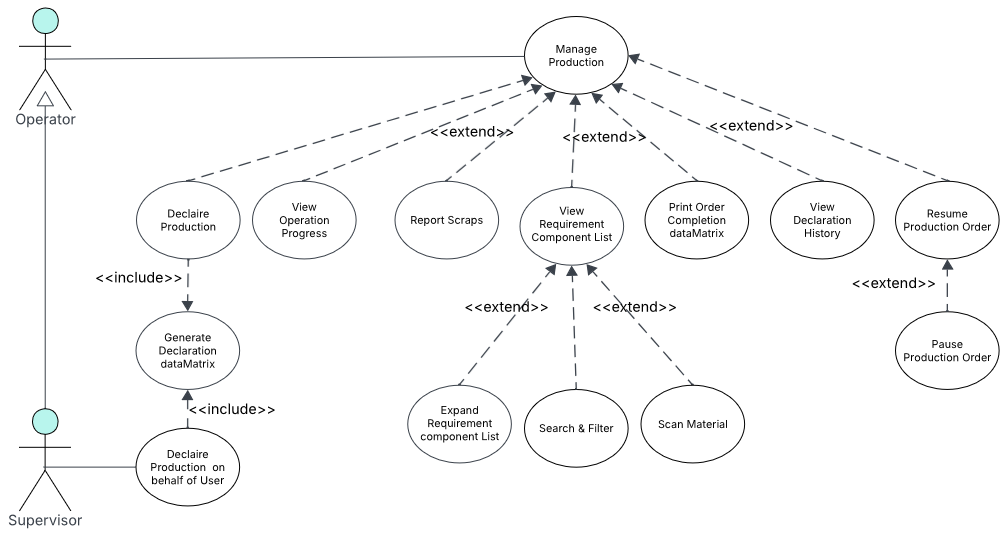
\includegraphics[width=\linewidth,keepaspectratio]{./media/MES_Sprint-3-Repport/diagrams/useCase/sprint3-1.png}
  \caption{UML Use Case Diagram --- Sprint 3 (manage production)}
  \label{fig:s3-uc-part1}
\end{figure}

\begin{figure}[H]
  \centering
  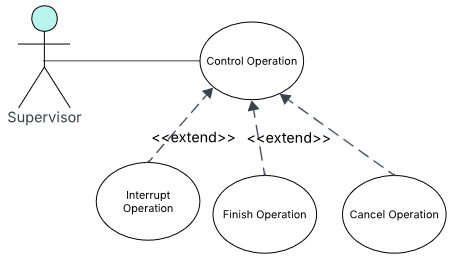
\includegraphics[height=0.35\textheight,keepaspectratio]{./media/MES_Sprint-3-Repport/diagrams/useCase/sprint3-2.png}
  \caption{UML Use Case Diagram --- Sprint 3 (control operations)}
  \label{fig:s3-uc-part2}
\end{figure}

\subsection{Textual Use Case Description}

\Needspace{10\baselineskip}
\begin{longtable}{@{} P{0.21\linewidth} P{0.75\linewidth} @{}}
	\caption{Textual Use Case Description --- Declare Production}
	\label{tab:s3-uc-declare-production} \\
	\toprule
	\endfirsthead
	\midrule
	\endhead
	
	\multicolumn{2}{r}{\small Continued on next page} \\
	\endfoot
	\bottomrule
	\endlastfoot
	
	\textbf{Use Case Name} & Declare Production \\
	\midrule
	\textbf{Primary Actor} & \userrole{Operator} / \userrole{Supervisor} \\
	\midrule
	\textbf{Preconditions} & 
	\begin{itemize}[noitemsep, topsep=0pt, partopsep=0pt, leftmargin=*]
	\item The user is authenticated and navigated to an Operation Detail page.
	\item The operation status is \domainterm{Running}.
	\item The produced quantity is below the order quantity.
	\end{itemize} \\
	\midrule
	\textbf{Postconditions} & 
	\begin{itemize}[noitemsep, topsep=0pt, partopsep=0pt, leftmargin=*]
	\item A new \techname{MES Operation Progression} record is inserted.
	\item The production chart and cycle table update via the refresh stream or trigger.
	\item The progress percentage and produced quantity in the info container update.
	\end{itemize} \\
	\midrule
	\textbf{Main Scenario} & 
	\begin{enumerate}[noitemsep, topsep=0pt, partopsep=0pt, leftmargin=*]
	\item The user taps \uilabel{Declare Production} in the Quick Actions panel.
	\item The \techname{DeclareProductionDialog} opens showing the remaining quantity.
	\item The user (if Supervisor) optionally selects an operator from the dropdown to declare on behalf of.
	\item The user enters a positive integer not exceeding the remaining quantity.
	\item The user taps \uilabel{Submit}.
	\item The ERP validates the quantity and inserts the progression record.
	\item The user is redirected to the declaration lable print page
	\item The refresh stream triggers a live data update.
	\end{enumerate} \\
	\midrule
	\textbf{Alternative Flow} & 
	\begin{itemize}[noitemsep, topsep=0pt, partopsep=0pt, leftmargin=*]
	\item \textit{Step 3, invalid quantity}: client-side validation shows an inline error; submission is blocked.
	\item \textit{Step 6, ERP error}: the server error message is displayed in the dialog; the record is not inserted.
	\end{itemize} \\
\end{longtable}


\bigskip

\Needspace{10\baselineskip}
\begin{longtable}{@{} P{0.21\linewidth} P{0.75\linewidth} @{}}
	\caption{Textual Use Case Description --- Finish / Cancel / Interrupt Operation}
	\label{tab:s3-uc-close-operation} \\
	\toprule
	\endfirsthead
	\midrule
	\endhead
	\multicolumn{2}{r}{\small Continued on next page} \\
	\endfoot
	\bottomrule
	\endlastfoot
	
	\textbf{Use Case Name} & Finish / Cancel / Interrupt Operation \\
	\midrule
	\textbf{Primary Actor} & \userrole{Supervisor} \\
	\midrule
	\textbf{Preconditions} & 
	\begin{itemize}[noitemsep, topsep=0pt, partopsep=0pt, leftmargin=*]
	\item The user is authenticated with an active session as a \userrole{Supervisor}.
	\item The operation is in \domainterm{Running}, \domainterm{Paused}, or \domainterm{Released and unstarted} state.
	\end{itemize} \\
	\midrule
	\textbf{Postconditions} & 
	\begin{itemize}[noitemsep, topsep=0pt, partopsep=0pt, leftmargin=*]
	\item A \domainterm{Finished}, \domainterm{Interrupted}, or \domainterm{Cancelled} status record is inserted.
	\item The execution end time is stamped.
	\item An Idle machine status record is inserted if the operation was started.
	\end{itemize} \\
	\midrule
	\textbf{Main Scenario} & 
	\begin{enumerate}[noitemsep, topsep=0pt, partopsep=0pt, leftmargin=*]
	\item The user clickes in the (Interrupt, Finish, Cancel) button based on the operation state.
	\item A confirmation dialog is displayed; the user confirms.
	\item The system POSTs to \apiendpoint{/MESWebService\_finishOperation} or \apiendpoint{cancelOperation}.
	\item The ERP validates, inserts the status record, stamps the end time, and inserts an Idle machine status.
	\end{enumerate} \\
\end{longtable}


\Needspace{10\baselineskip}
\begin{longtable}{@{} P{0.21\linewidth} P{0.75\linewidth} @{}}
    \caption{Textual Use Case Description --- Scan Component Consumption}
    \label{tab:s3-uc-scan-component-consumption} \\
    \toprule
    \endfirsthead
    \midrule
    \endhead
    \multicolumn{2}{r}{\small Continued on next page} \\
    \endfoot
    \bottomrule
    \endlastfoot

    \textbf{Use Case Name} & Scan Component Consumption \\
    \midrule
    \textbf{Primary Actor} & \userrole{Operator} / \userrole{Supervisor} \\
    \midrule
    \textbf{Preconditions} &
    \begin{itemize}[noitemsep, topsep=0pt, partopsep=0pt, leftmargin=*]
        \item The user is authenticated and holds a valid session token.
        \item The operation has been started.
        \item The user is on the Operation Detail page with the \techname{ScannerWidget} open.
    \end{itemize} \\
    \midrule
    \textbf{Postconditions} &
    \begin{itemize}[noitemsep, topsep=0pt, partopsep=0pt, leftmargin=*]
        \item One \techname{MES Operation Scan} record is inserted per scanned item line.
        \item One \techname{Item Journal Line} (consumption) is posted to BC inventory per scanned item line.
        \item The \techname{Required Component} widget refreshes to reflect the updated consumed quantities.
    \end{itemize} \\
    \midrule
    \textbf{Main Scenario} &
    \begin{enumerate}[noitemsep, topsep=0pt, partopsep=0pt, leftmargin=*]
        \item The user taps \uilabel{Scan Item} and points the camera or scanner at a component barcode.
        \item Flutter POSTs to \apiendpoint{/api/resolveBarcode}; the middleware forwards the call to \techname{MESWebService\_resolveBarcode} in AL.
        \item AL resolves the item: if the barcode carries an \texttt{Item Number:} prefix, AL parses the item number directly and retrieves the item record from BC; otherwise AL resolves the identifier via the \techname{Item Identifier} table.
        \item AL fetches the unit-of-measure conversion factor via \texttt{Item Unit of Measure.Get} and returns \texttt{itemNo}, \texttt{itemDescription}, \texttt{unitOfMeasure}, and \texttt{quantityPerUnitOfMeasure} to Flutter.
        \item Flutter validates the response and adds the item to the local scanned-items list (or increments its quantity if already present); the item appears in the scan list.
        \item The user repeats steps 1--5 for each additional component, then taps \uilabel{Confirm Scans}.
        \item Flutter POSTs the full scan list to \apiendpoint{/api/insertScans}; the middleware forwards to \techname{MESWebService\_insertScans} in AL.
        \item AL for each scan inserts an \techname{MES Operation Scan} record and an \techname{Item Journal Line}.
        \item AL posts all journal lines to BC inventory in a single batch; BC confirms success.
        \item Flutter pops the \techname{ScannerWidget} and triggers a data refresh; the \techname{Required Component} widget displays the updated consumed quantities.
    \end{enumerate} \\
    \midrule
    \textbf{Alternative Flow} &
    \begin{itemize}[noitemsep, topsep=0pt, partopsep=0pt, leftmargin=*]
        \item \textit{Step 3, unresolvable barcode}: AL returns an error; Flutter displays an inline error message and does not add the item to the scan list.
        \item \textit{Step 5, client validation failure}: Flutter blocks the addition and shows an inline error (e.g.\ zero or negative quantity).
        \item \textit{Step 9, BC posting error}: AL returns the server error to Flutter; no consumption or journal records are committed, and the dialog remains open with the error displayed.
    \end{itemize} \\
\end{longtable}
\bigskip

\subsection{Sequence Diagrams}

The following sequence diagrams illustrate the communication flow between the
\techname{Flutter} frontend, the \techname{Business Central} OData layer, and
the \techname{AL} business logic for the production and operation-lifecycle
flows introduced in Sprint~3.

% Figure~\ref{fig:s3-seq-declare-production} depicts the production declaration
% flow. The operator submits a quantity; the \techname{Flutter} client validates
% the input locally, then forwards the request to the \techname{AL} layer,
% which re-validates the token (SD-02), checks that the declared amount is
% positive and does not exceed the remaining order quantity, and — on success —
% inserts a new immutable \domainterm{MES Operation Progression} record and
% records the relevant user interaction entries. When a \userrole{Supervisor}
% declares production on behalf of an operator, the \techname{AL} layer
% additionally verifies that the two users share at least one work centre before
% proceeding.

% \begin{figure}[H]
%   \centering
%   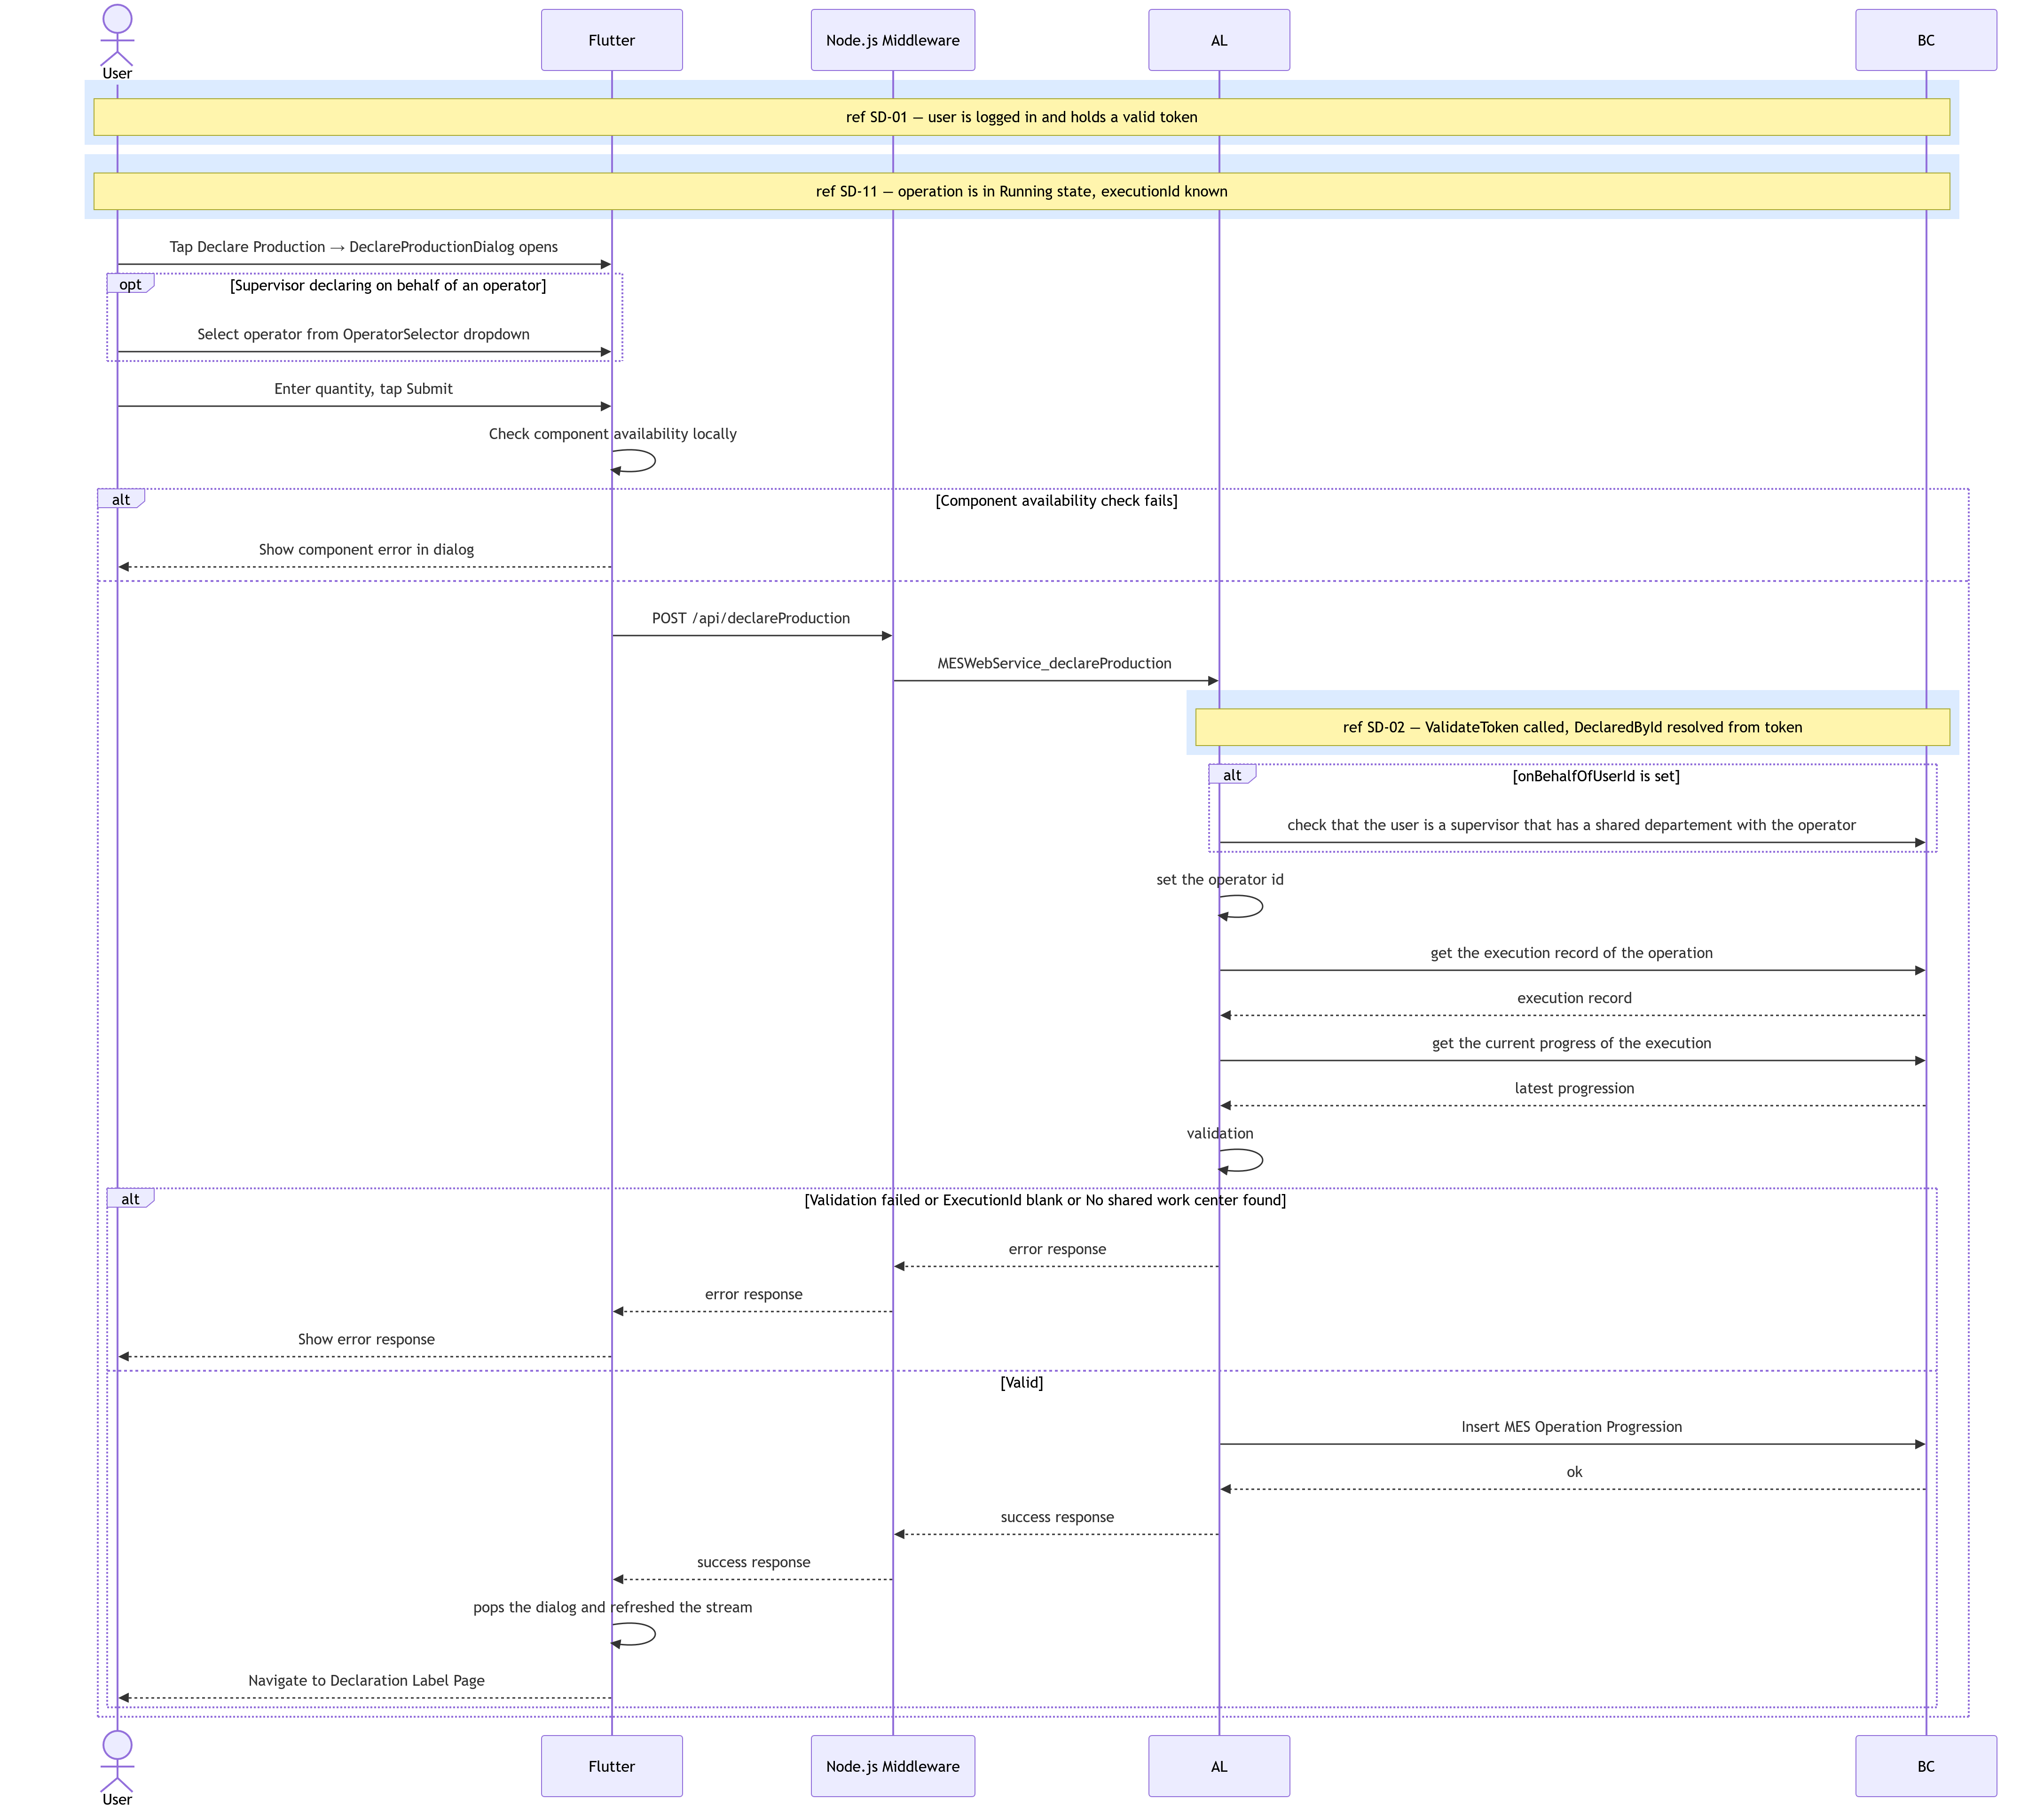
\includegraphics[width=\linewidth,height=0.82\textheight,keepaspectratio]{./media/MES_Sprint-3-Repport/diagrams/sequence/declare-production.png}
%   \caption{SD-12: Declare Production.}
%   \label{fig:s3-seq-declare-production}
% \end{figure}


%=====SD-12==========================================================
% sequenceDiagram
%     actor User
%     participant Flutter
%     participant Node as Node.js Middleware
%     participant AL
%     participant BC

%     rect rgb(220,235,255)
%         Note over User,BC: ref SD-01 — user is logged in and holds a valid token
%     end
%     rect rgb(220,235,255)
%         Note over User,BC: ref SD-11 — operation is in Running state, executionId known
%     end

%     User->>Flutter: Tap Declare Production → DeclareProductionDialog opens
%     opt Supervisor declaring on behalf of an operator
%         User->>Flutter: Select operator from OperatorSelector dropdown
%     end
%     User->>Flutter: Enter quantity, tap Submit
%     Flutter->>Flutter: Check component availability locally
%     alt Component availability check fails
%         Flutter-->>User: Show component error in dialog
%     else
%         Flutter->>Node: POST /api/declareProduction
%         Node->>AL: MESWebService_declareProduction
%         rect rgb(220,235,255)
%             Note over AL,BC: ref SD-02 — ValidateToken called, DeclaredById resolved from token
%         end
%         alt onBehalfOfUserId is set
%             AL->>BC: check that the user is a supervisor that has a shared departement with the operator
%         end
%         AL->>AL: set the operator id

%         AL->>BC: get the execution record of the operation
%         BC-->>AL: execution record 
%         AL->>BC: get the current progress of the execution
%         BC-->>AL: latest progression 
%         AL->>AL: validation
%         alt Validation failed or ExecutionId blank or No shared work center found
%             AL-->>Node: error response
%             Node-->>Flutter: error response
%             Flutter-->>User: Show error response
%         else Valid
%             AL->>BC: Insert MES Operation Progression
%             BC-->>AL: ok
%             AL-->>Node: success response
%             Node-->>Flutter: success response
%             Flutter->>Flutter: pops the dialog and refreshed the stream
%             Flutter-->>User: Navigate to Declaration Label Page
%         end
%     end
%====================================================================


Figures~\ref{fig:s3-seq-fetch-bom} and~\ref{fig:s3-seq-fetch-production-cycle}
present the two supplementary data-retrieval flows that run concurrently
alongside the main operation detail view. Both are polling streams that
re-emit on demand or when a state-change trigger is received from the
\techname{Flutter} client.
 
Figure~\ref{fig:s3-seq-fetch-bom} describes the bill-of-materials retrieval
flow. The \techname{AL} layer resolves the routing link code from the active
\domainterm{ProdOrderRoutingLine}, filters the production order components
by that link, aggregates the quantity already scanned per item, and resolves
per-unit quantities from the \domainterm{ItemUnitOfMeasure} table before
returning the assembled BOM rows to the \techname{Flutter} client.

\begin{figure}[H]
  \centering
  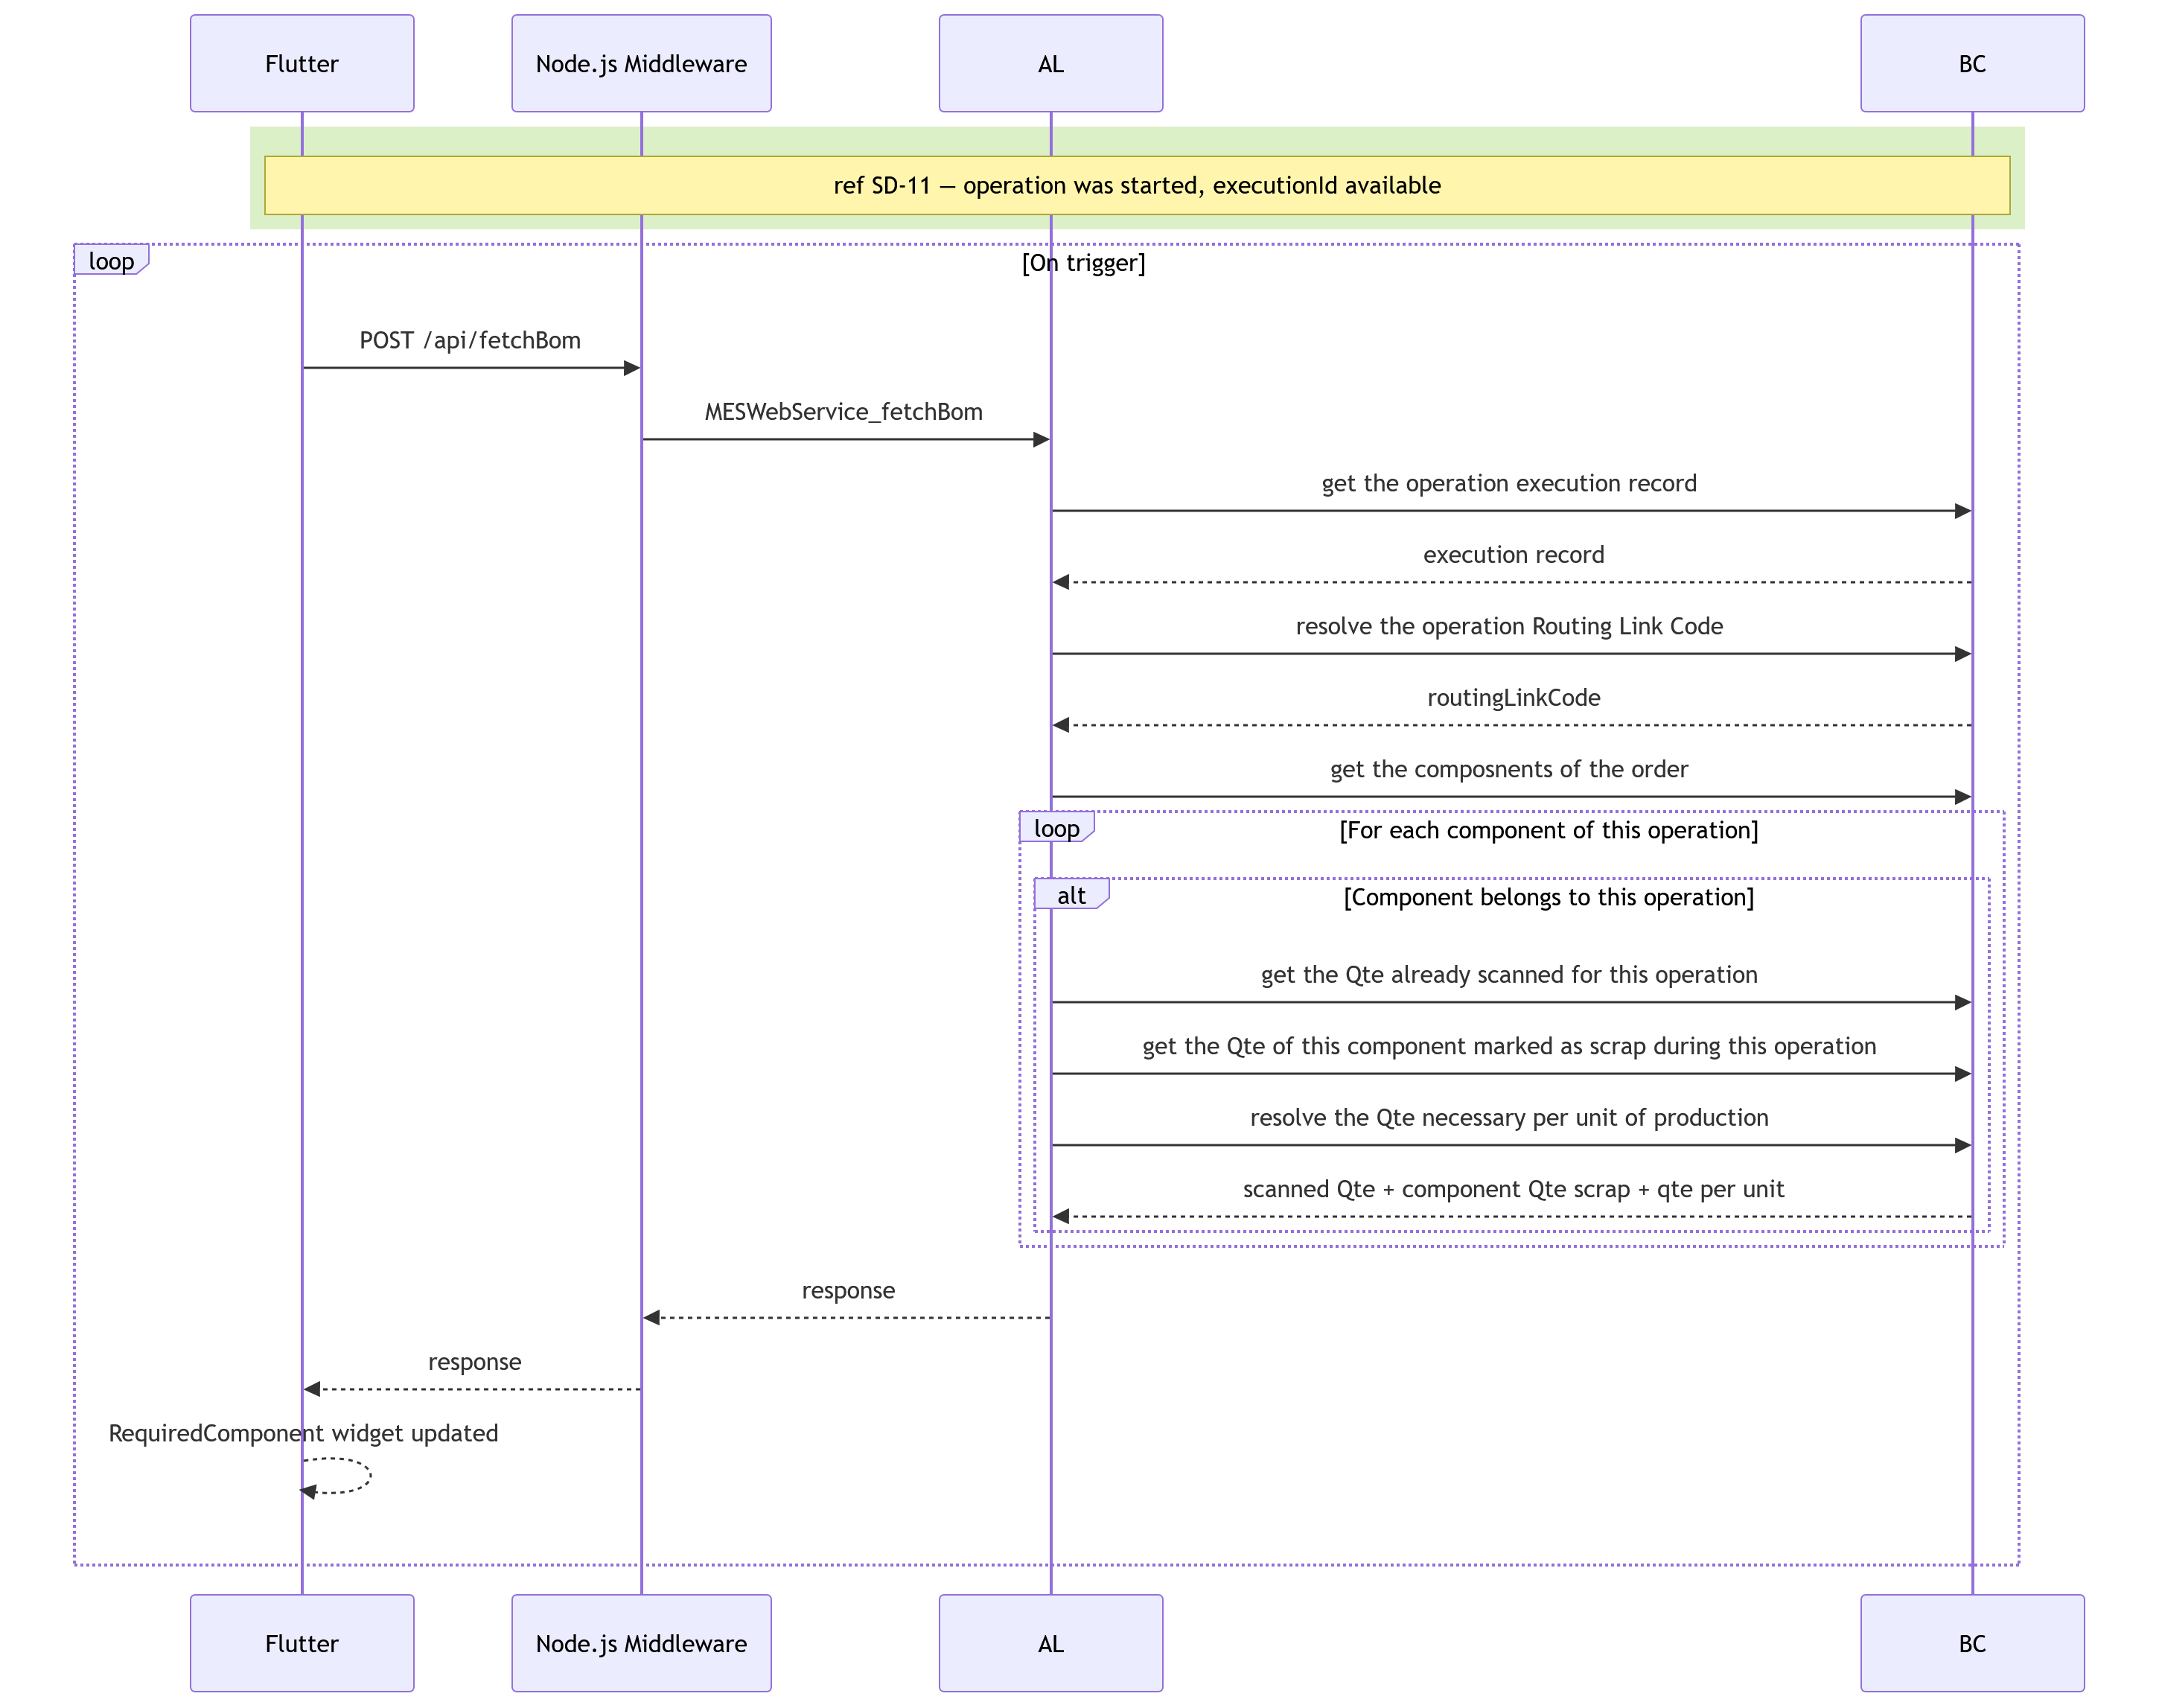
\includegraphics[width=\linewidth,height=0.82\textheight,keepaspectratio]{./media/MES_Sprint-3-Repport/diagrams/sequence/fetch-BOM.png}
  \caption{SD-21: Fetch Bill of Materials.}
  \label{fig:s3-seq-fetch-bom}
\end{figure}

%=====SD-21==========================================================
%  sequenceDiagram
%       participant Flutter
%       participant Node as Node.js Middleware
%       participant AL
%       participant BC

%       rect rgb(220,240,200)
%           Note over Flutter,BC: ref SD-11 — operation was started, executionId available
%       end

%       loop On trigger
%           Flutter->>Node: POST /api/fetchBom 
%           Node->>AL: MESWebService_fetchBom 

%           AL->>BC:get the operation execution record
%           BC-->>AL: execution record 
%           AL->>BC: resolve the operation Routing Link Code
%           BC-->>AL: routingLinkCode
%           AL->>BC: get the composnents of the order
%           loop For each component of this operation
%              alt Component belongs to this operation
%                   AL->>BC: get the Qte already scanned for this operation 
%                   AL->>BC: get the Qte of this component marked as scrap during this operation
%                   AL->>BC: resolve the Qte necessary per unit of production
%                   BC-->>AL: scanned Qte + component Qte scrap + qte per unit
%               end
%           end

%           AL-->>Node: response
%           Node-->>Flutter: response
%           Flutter-->>Flutter: RequiredComponent widget updated
%       end
%====================================================================

Figure~\ref{fig:s3-seq-fetch-production-cycle} illustrates the production-cycle
retrieval flow. The \techname{AL} layer fetches the full progression history
for the operation, enriches each entry with the name of the user who declared
it, and returns the assembled cycle list to the \techname{Flutter} client.

\begin{figure}[H]
  \centering
  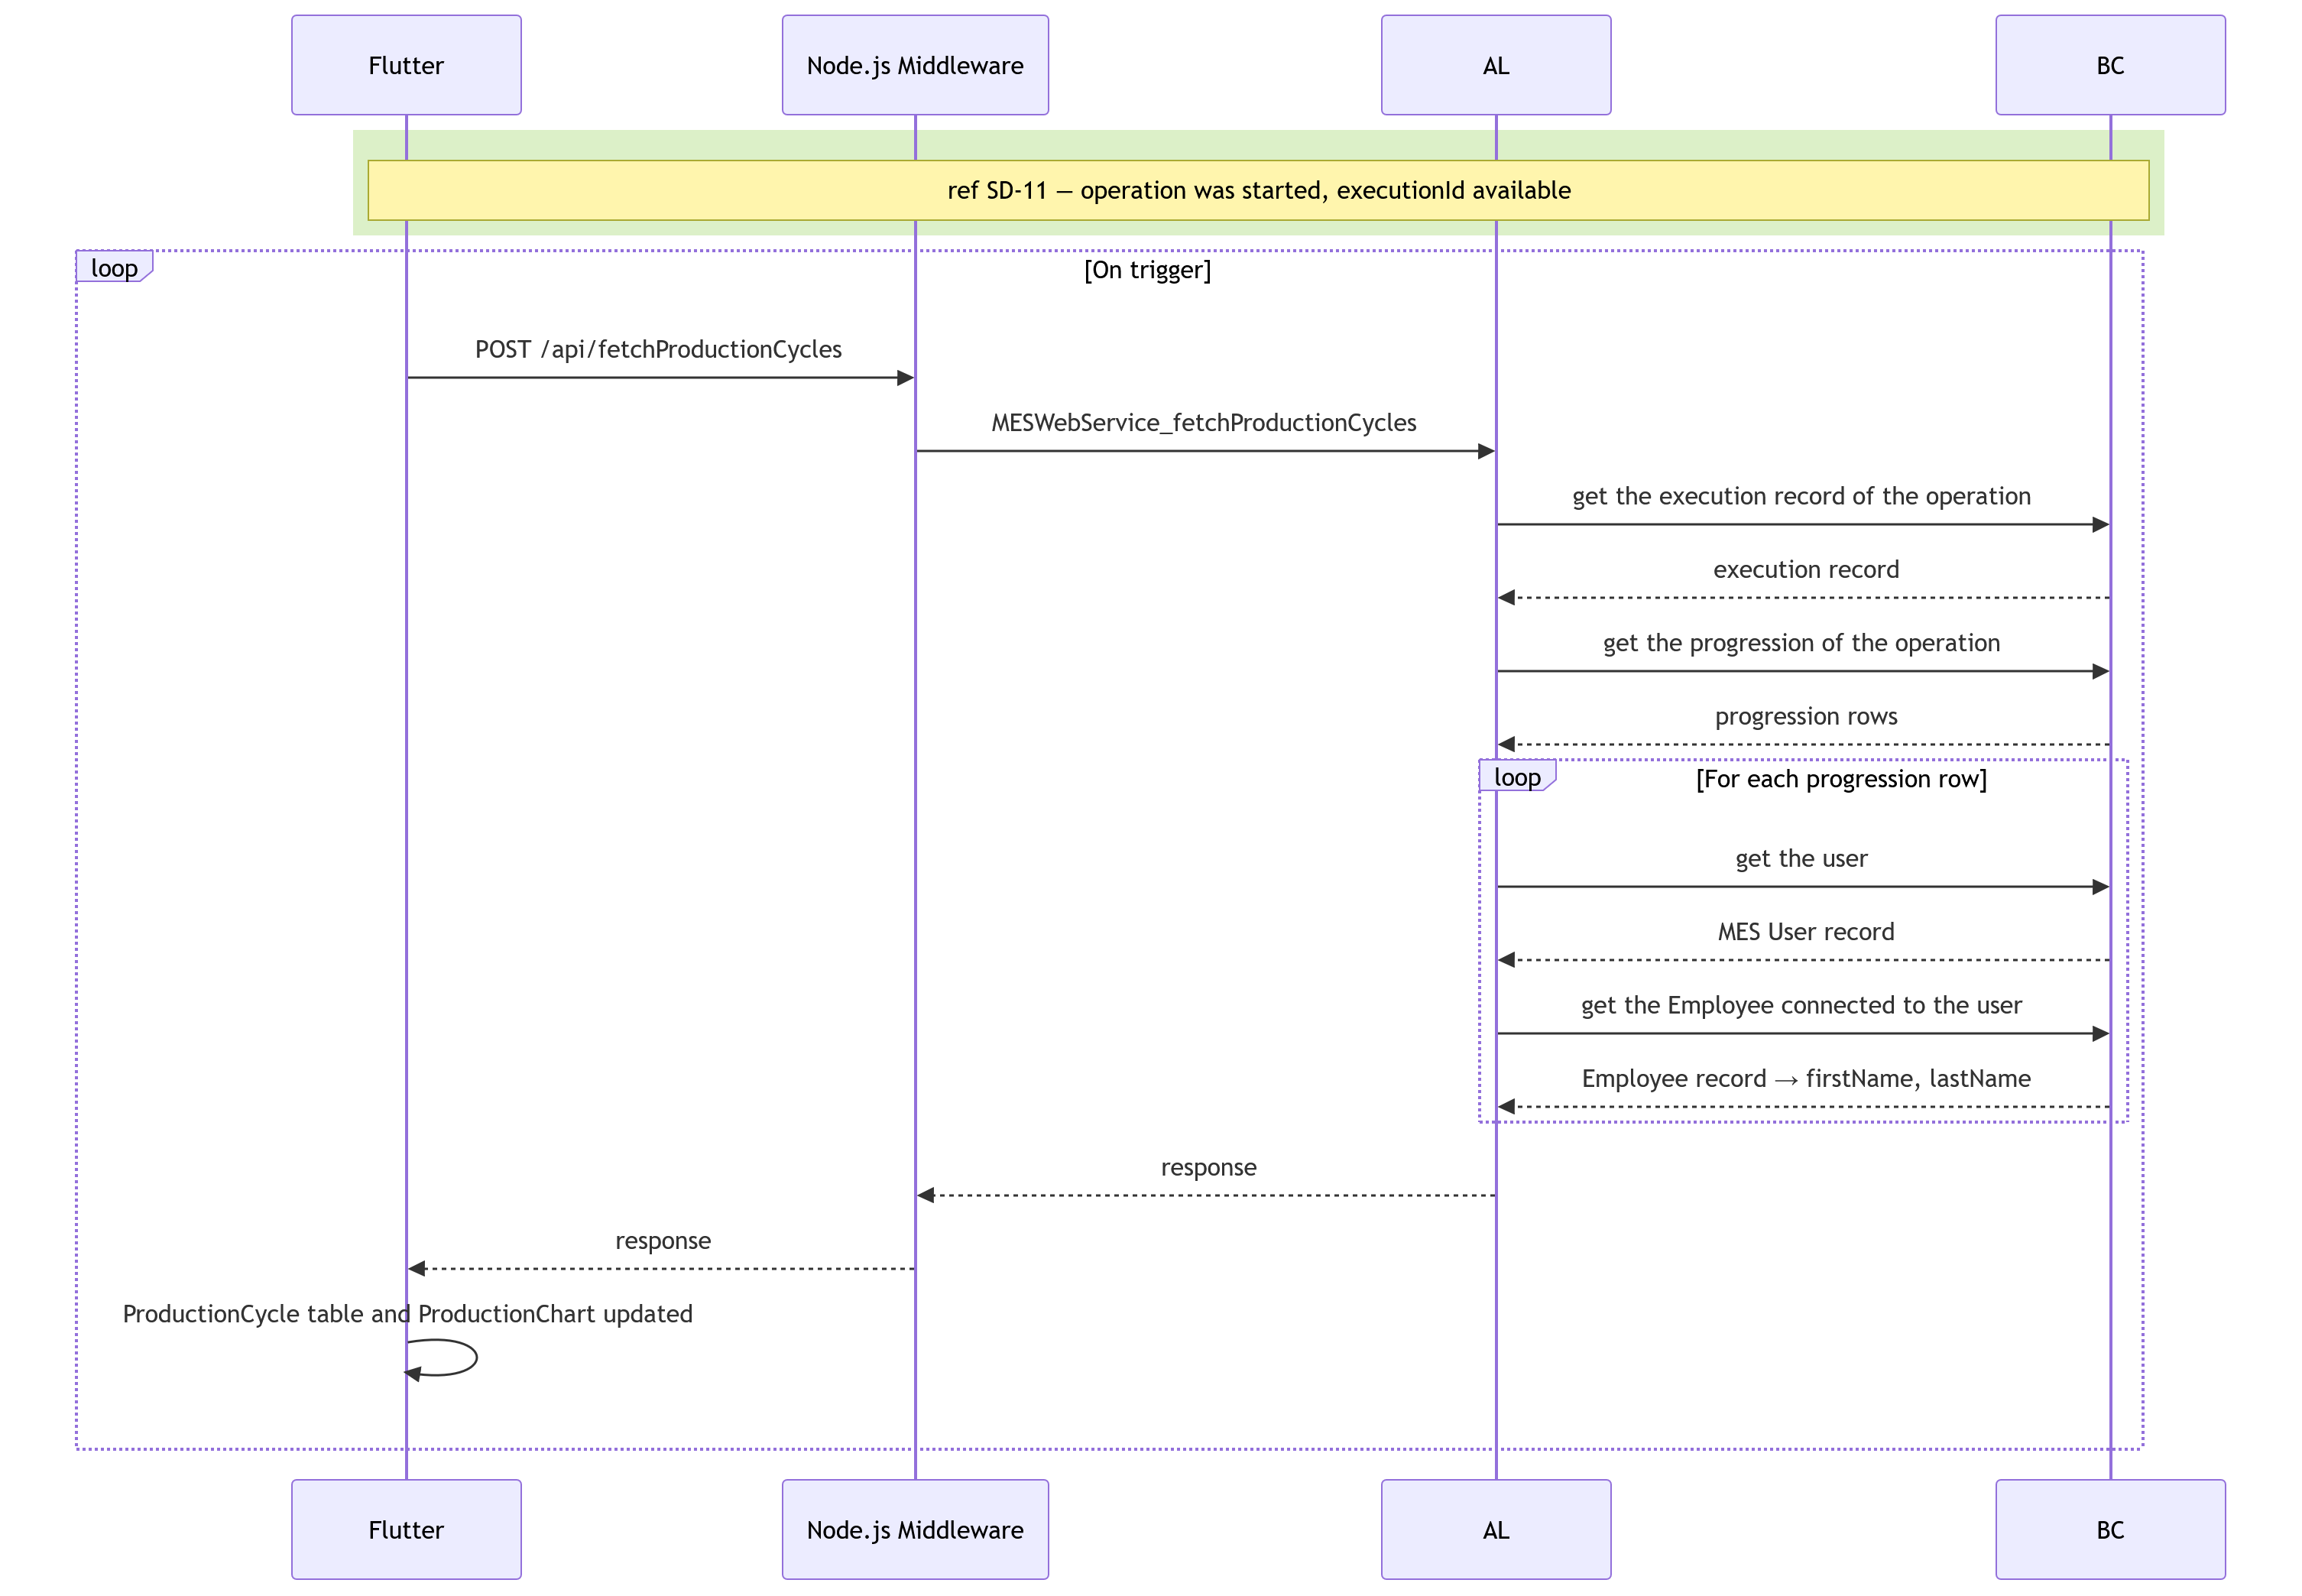
\includegraphics[width=\linewidth,height=0.82\textheight,keepaspectratio]{./media/MES_Sprint-3-Repport/diagrams/sequence/fetch-production-cycle.png}
  \caption{SD-22: Fetch Production Cycles.}
  \label{fig:s3-seq-fetch-production-cycle}
\end{figure}

%=====SD-22==========================================================
% sequenceDiagram
%       participant Flutter
%       participant Node as Node.js Middleware
%       participant AL
%       participant BC

%       rect rgb(220,240,200)
%           Note over Flutter,BC: ref SD-11 — operation was started, executionId available
%       end

%       loop On trigger
%           Flutter->>Node: POST /api/fetchProductionCycles 
%           Node->>AL: MESWebService_fetchProductionCycles 

%           AL->>BC: get the execution record of the operation
%           BC-->>AL: execution record 
%           AL->>BC: get the progression of the operation
%           BC-->>AL: progression rows

%           loop For each progression row
%               AL->>BC: get the user
%               BC-->>AL: MES User record
%               AL->>BC: get the Employee connected to the user
%               BC-->>AL: Employee record → firstName, lastName
%           end

%           AL-->>Node: response
%           Node-->>Flutter: response
%           Flutter->>Flutter: ProductionCycle table and ProductionChart updated
%       end
%====================================================================

Figures~\ref{fig:s3-seq-pause-operation} through~\ref{fig:s3-seq-resume-operation}
illustrate the operation: pause, resume. Figure~\ref{fig:s3-seq-pause-operation} describes the pause flow. The
\techname{AL} layer confirms that the operation is currently in the
\domainterm{Running} state before inserting a \domainterm{Paused}
\domainterm{MES Operation State} record and setting the machine status
back to \domainterm{Idle}.

\begin{figure}[H]
  \centering
  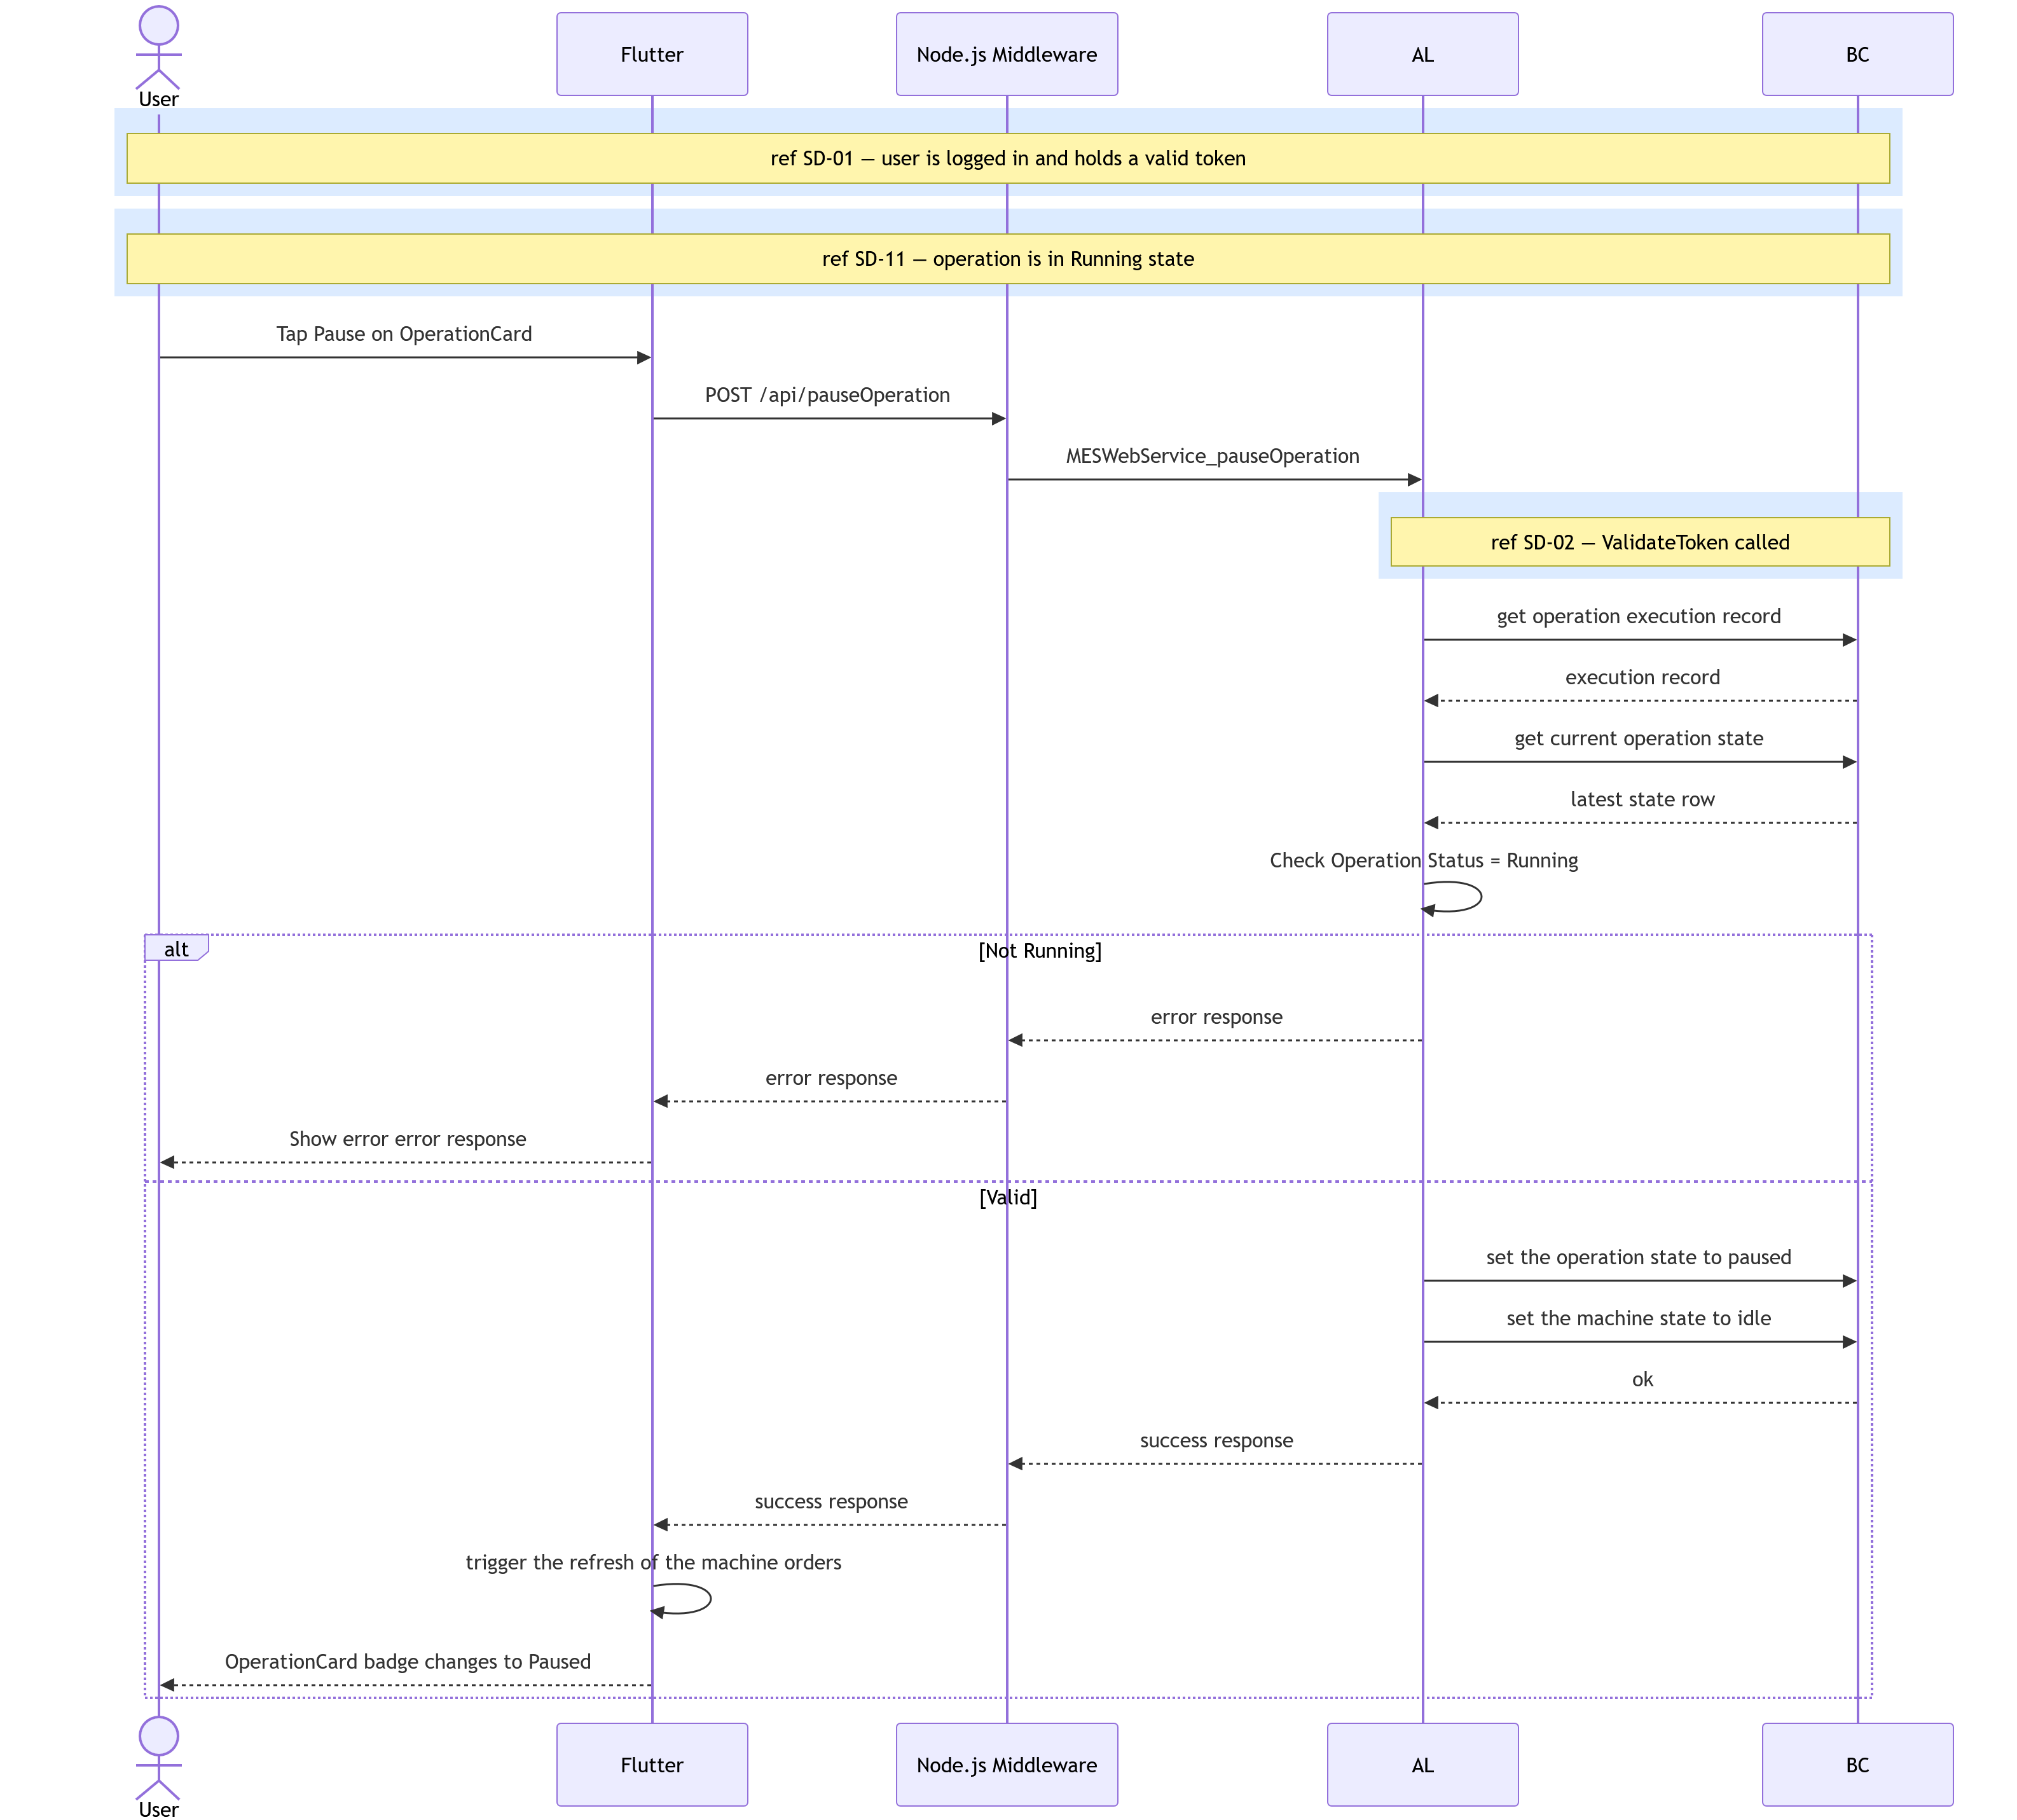
\includegraphics[width=\linewidth,height=0.82\textheight,keepaspectratio]{./media/MES_Sprint-3-Repport/diagrams/sequence/pause-operation.png}
  \caption{SD-13: Pause Operation.}
  \label{fig:s3-seq-pause-operation}
\end{figure}

%=====SD-13==========================================================
% sequenceDiagram
%       actor User
%       participant Flutter
%       participant Node as Node.js Middleware
%       participant AL
%       participant BC

%       rect rgb(220,235,255)
%           Note over User,BC: ref SD-01 — user is logged in and holds a valid token
%       end
%       rect rgb(220,235,255)
%           Note over User,BC: ref SD-11 — operation is in Running state
%       end

%       User->>Flutter: Tap Pause on OperationCard
%       Flutter->>Node: POST /api/pauseOperation
%       Node->>AL: MESWebService_pauseOperation 

%       rect rgb(220,235,255)
%           Note over AL,BC: ref SD-02 — ValidateToken called
%       end

%       AL->>BC: get operation execution record
%       BC-->>AL: execution record 
%       AL->>BC: get current operation state 
%       BC-->>AL: latest state row
%       AL->>AL: Check Operation Status = Running
%       alt Not Running
%           AL-->>Node: error response
%           Node-->>Flutter: error response
%           Flutter-->>User: Show error error response
%       else Valid
%           AL->>BC: set the operation state to paused
%           AL->>BC: set the machine state to idle
%           BC-->>AL: ok
%           AL-->>Node: success response
%           Node-->>Flutter: success response
%           Flutter->>Flutter: trigger the refresh of the machine orders
%           Flutter-->>User: OperationCard badge changes to Paused
%       end
%====================================================================

Figure~\ref{fig:s3-seq-resume-operation} presents the resume flow. In addition
to confirming that the operation is in the \domainterm{Paused} state, the
\techname{AL} layer verifies that no other operation is currently running on
the same machine before inserting a \domainterm{Running} state record and
marking the machine as \domainterm{Working}.

\begin{figure}[H]
  \centering
  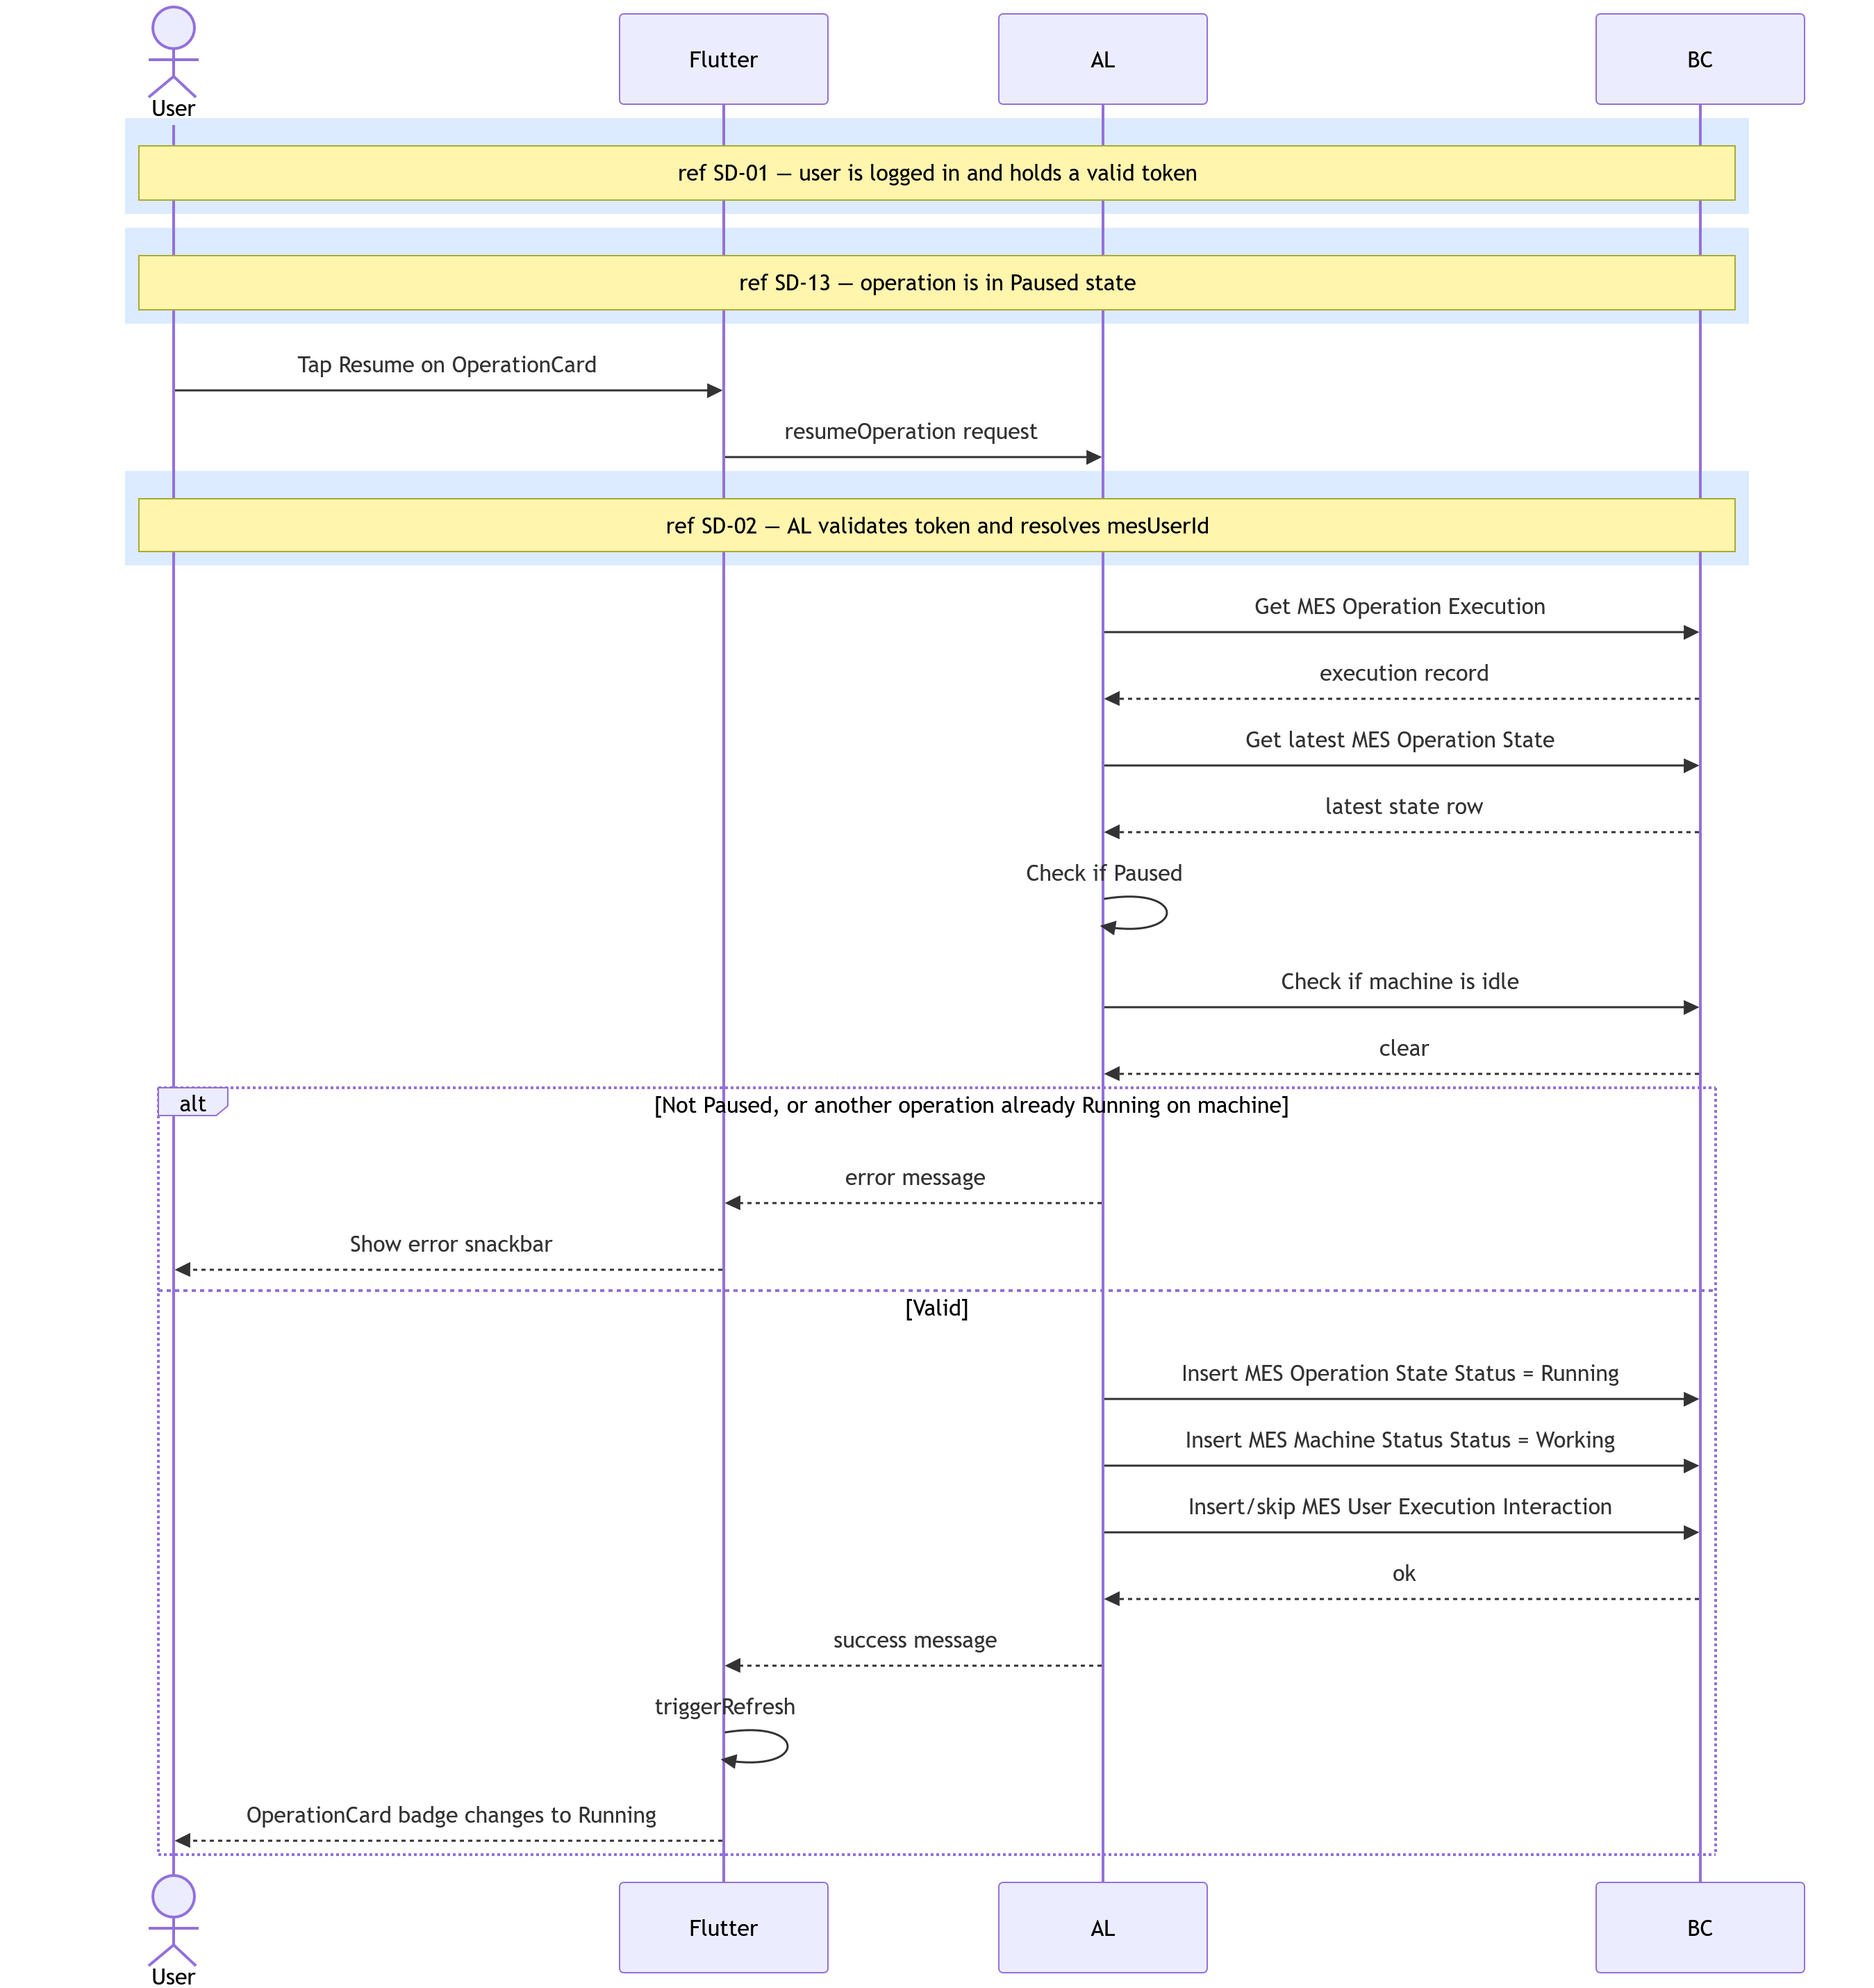
\includegraphics[width=\linewidth,height=0.82\textheight,keepaspectratio]{./media/MES_Sprint-3-Repport/diagrams/sequence/resume-operation.png}
  \caption{SD-14: Resume Operation.}
  \label{fig:s3-seq-resume-operation}
\end{figure}

%=====SD-14==========================================================
% sequenceDiagram
%       actor User
%       participant Flutter
%       participant Node as Node.js Middleware
%       participant AL
%       participant BC

%       rect rgb(220,235,255)
%           Note over User,BC: ref SD-01 — user is logged in and holds a valid token
%       end
%       rect rgb(220,235,255)
%           Note over User,BC: ref SD-13 — operation is in Paused state
%       end

%       User->>Flutter: Tap Resume on OperationCard
%       Flutter->>Node: POST /api/resumeOperation 
%       Node->>AL: MESWebService_resumeOperation 

%       rect rgb(220,235,255)
%           Note over AL,BC: ref SD-02 — ValidateToken called
%       end

%       AL->>BC: get the execution record of the operation
%       BC-->>AL: execution record 
%       AL->>BC: get the state of the operation
%       BC-->>AL: latest state row
%       AL->>AL: check if the operation is Paused
%       AL->>BC: check if the machine is idle
%       BC-->>AL: clear
%       alt Another operation is Running on machine or Not Paused
%           AL-->>Node: error response
%           Node-->>Flutter: error response
%           Flutter-->>User: Show error response
%       else Valid
%           AL->>BC: set the operation to running
%           AL->>BC: set machine to working
%           BC-->>AL: ok
%           AL-->>Node: success response
%           Node-->>Flutter: success response
%           Flutter->>Flutter: trigger refresh
%           Flutter-->>User: OperationCard badge updates
%       end
%====================================================================

Figure~\ref{fig:s3-seq-finish_cancel_interupt-operation} covers the finish and cancel
flows, which share a single endpoint family. The \techname{AL} layer rejects
the request if the operation is already in a terminal state; otherwise it
inserts the appropriate closed-state record, stamps the execution end time,
and resets the machine status to \domainterm{Idle}. The closed operation then
appears in the history view rather than the active operations list.	

\begin{figure}[H]
  \centering
  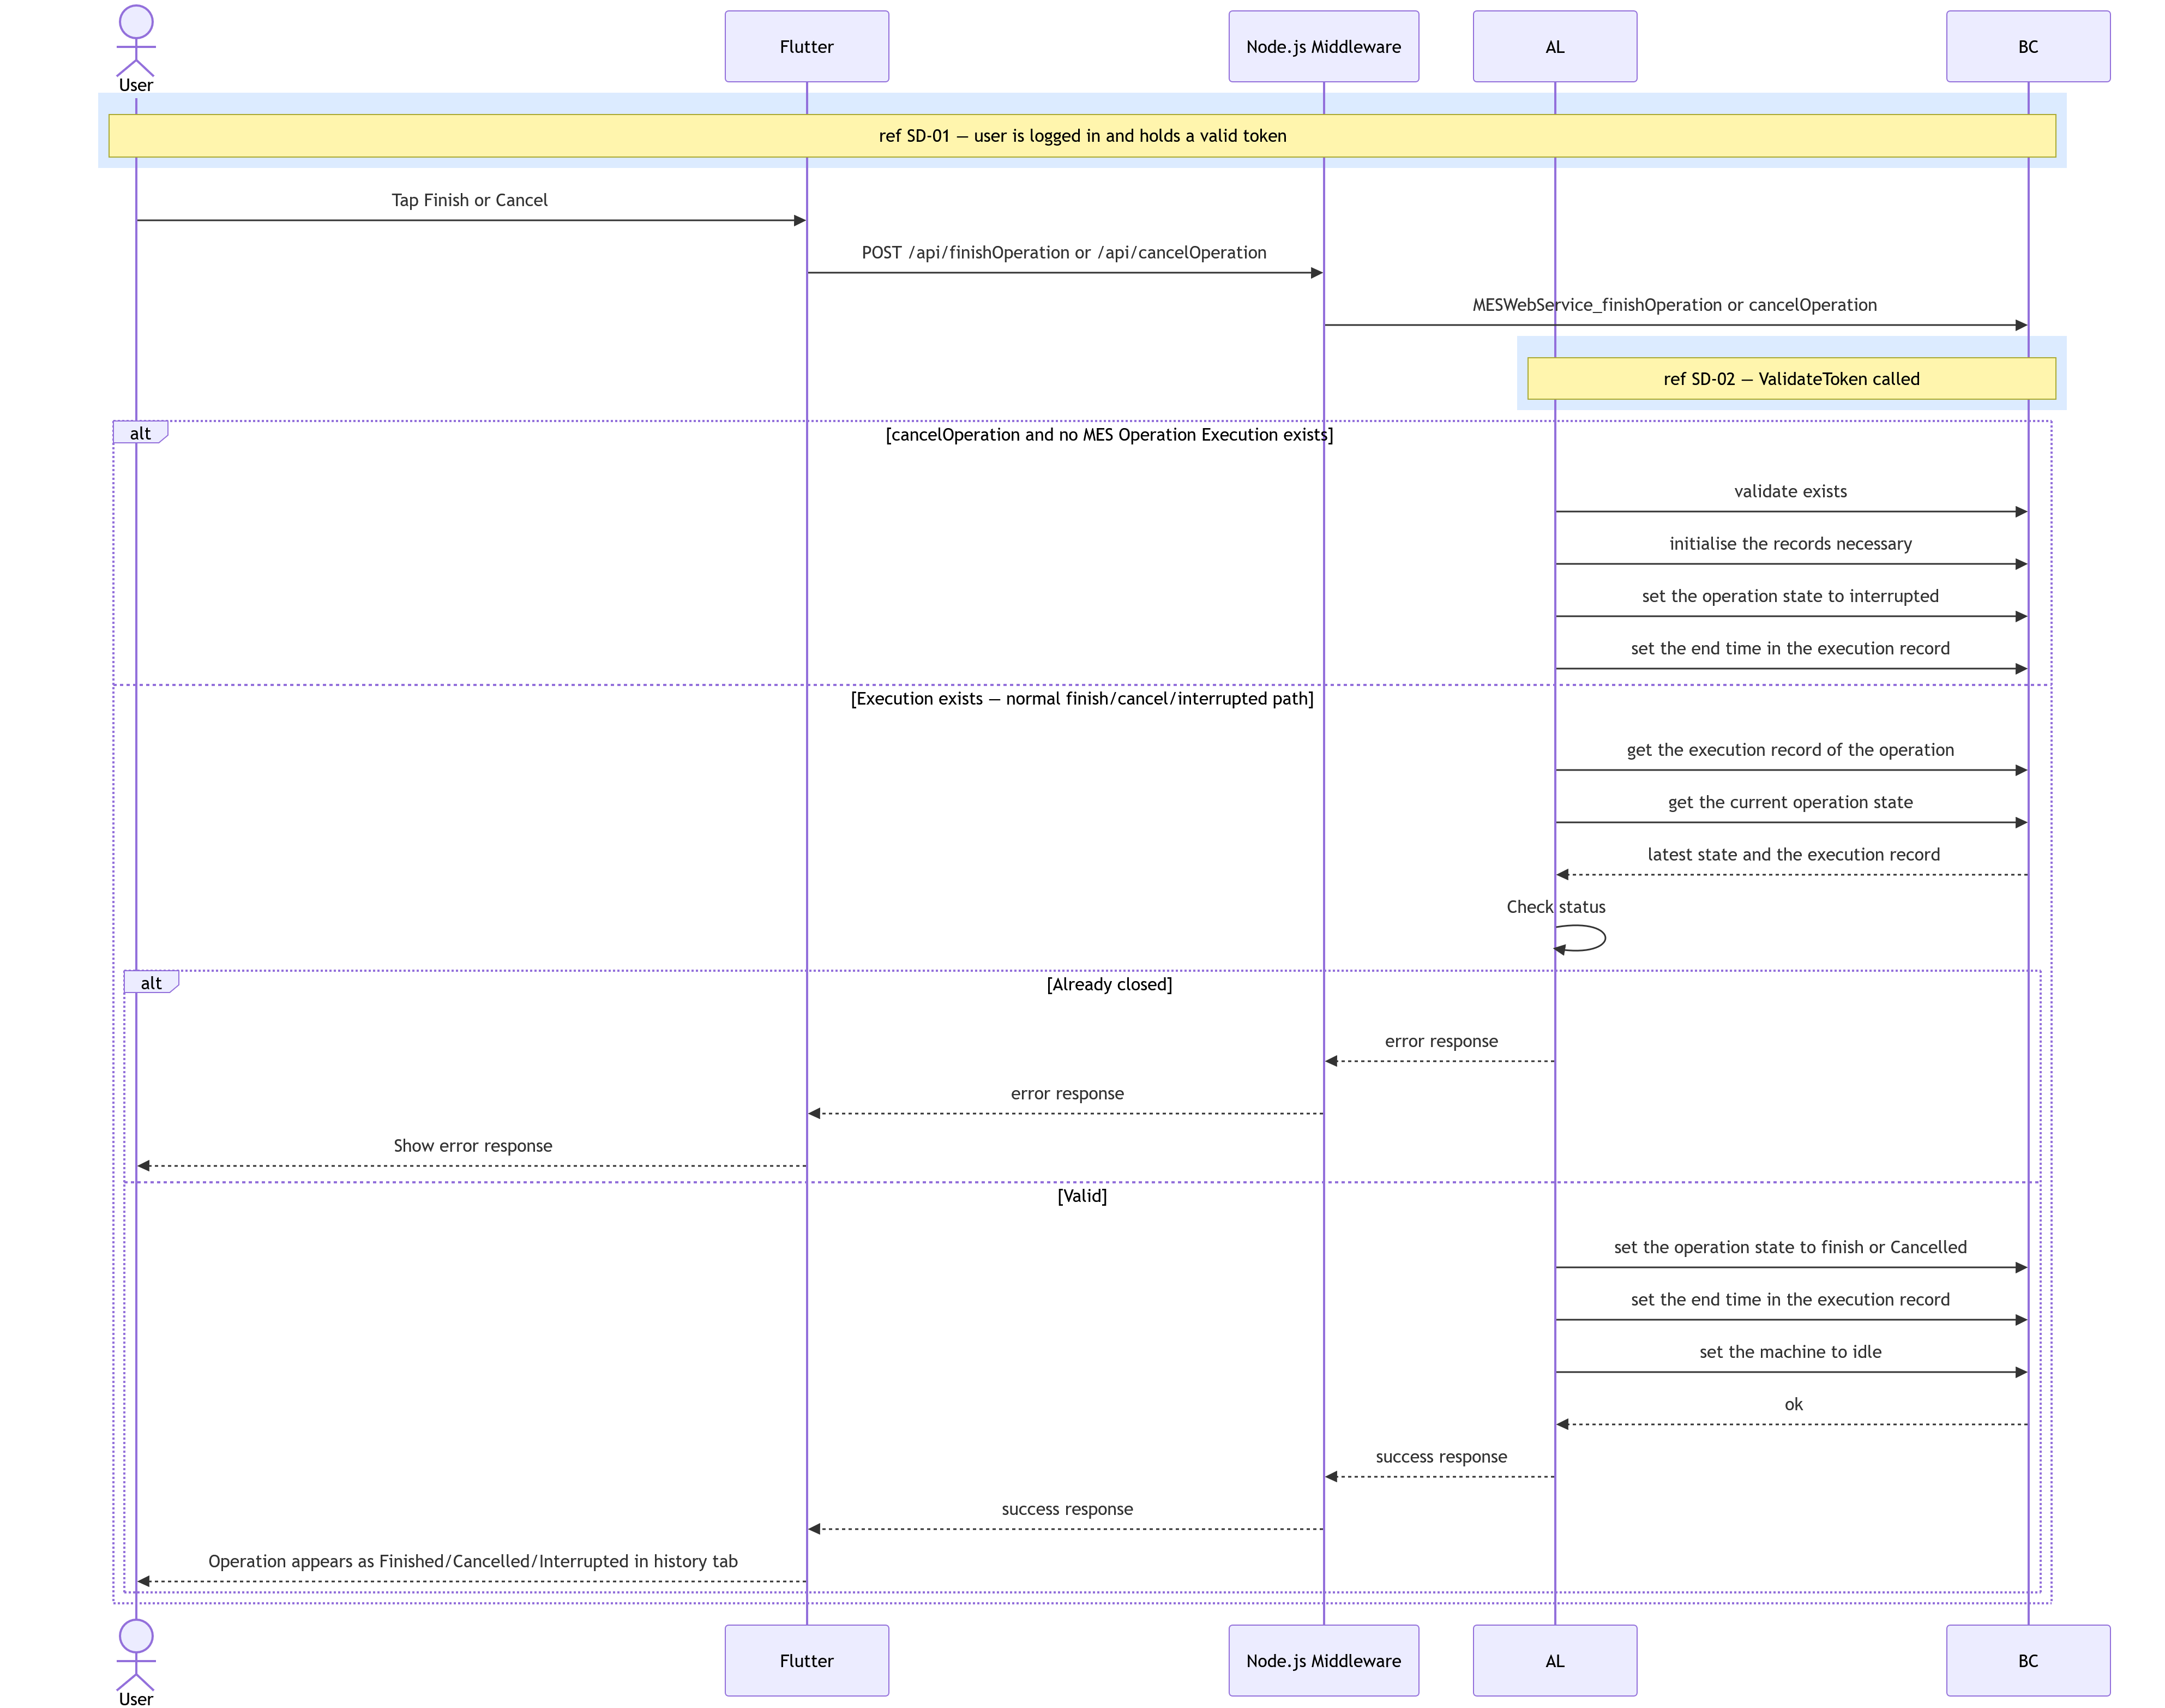
\includegraphics[width=\linewidth,height=0.82\textheight,keepaspectratio]{./media/MES_Sprint-3-Repport/diagrams/sequence/finish_cancel_interrupt-operation.png}
  \caption{SD-15: Finish/Cancel/Interrupt Operation.}
  \label{fig:s3-seq-finish_cancel_interupt-operation}
\end{figure}

%=====SD-15==========================================================
% sequenceDiagram
%     actor User
%     participant Flutter
%     participant AL
%     participant BC

%     rect rgb(220,235,255)
%         Note over User,BC: ref SD-01 — user is logged in and holds a valid token
%     end
%     rect rgb(220,235,255)
%         Note over User,BC: ref SD-11 — operation was started (Running or Paused)
%     end

%     User->>Flutter: Tap Finish (or Cancel)
%     Flutter->>AL: finishOperation or cancelOperation request

%     rect rgb(220,235,255)
%         Note over User,BC: ref SD-02 — AL validates token and resolves mesUserId
%     end

%     AL->>BC: Get MES Operation Execution
%     BC-->>AL: execution record
%     AL->>BC: Get latest MES Operation State
%     BC-->>AL: latest state
%     AL->>AL: Check if Finished or Cancelled
%     alt Already closed
%         AL-->>Flutter: error message
%         Flutter-->>User: Show error snackbar
%     else Valid
%         AL->>BC: Insert MES Operation State Status = Finished/Cancelled
%         AL->>BC: Update MES Operation Execution — set EndTime = now
%         AL->>BC: Insert MES Machine Status Status = Idle
%         AL->>BC: Insert/skip MES User Execution Interaction
%         BC-->>AL: ok
%         AL-->>Flutter: success message
%         Flutter-->>User: Operation appears as Finished/Cancelled in history
%     end
%====================================================================

% Figure~\ref{fig:s3-seq-declare-scrap} describes the scrap declaration flow.
% Before inserting the scrap record, the \techname{AL} layer verifies that
% the operation has not already been finished, cancelled, or paused, and that
% the referenced scrap code exists in \techname{Business Central}. On success,
% it inserts a \domainterm{MES Operation Scrap} entry, records user interaction,
% and appends a new \domainterm{MES Operation Progression} row so that the
% scrap quantity is reflected in the live data stream.

% \begin{figure}[H]
%   \centering
%   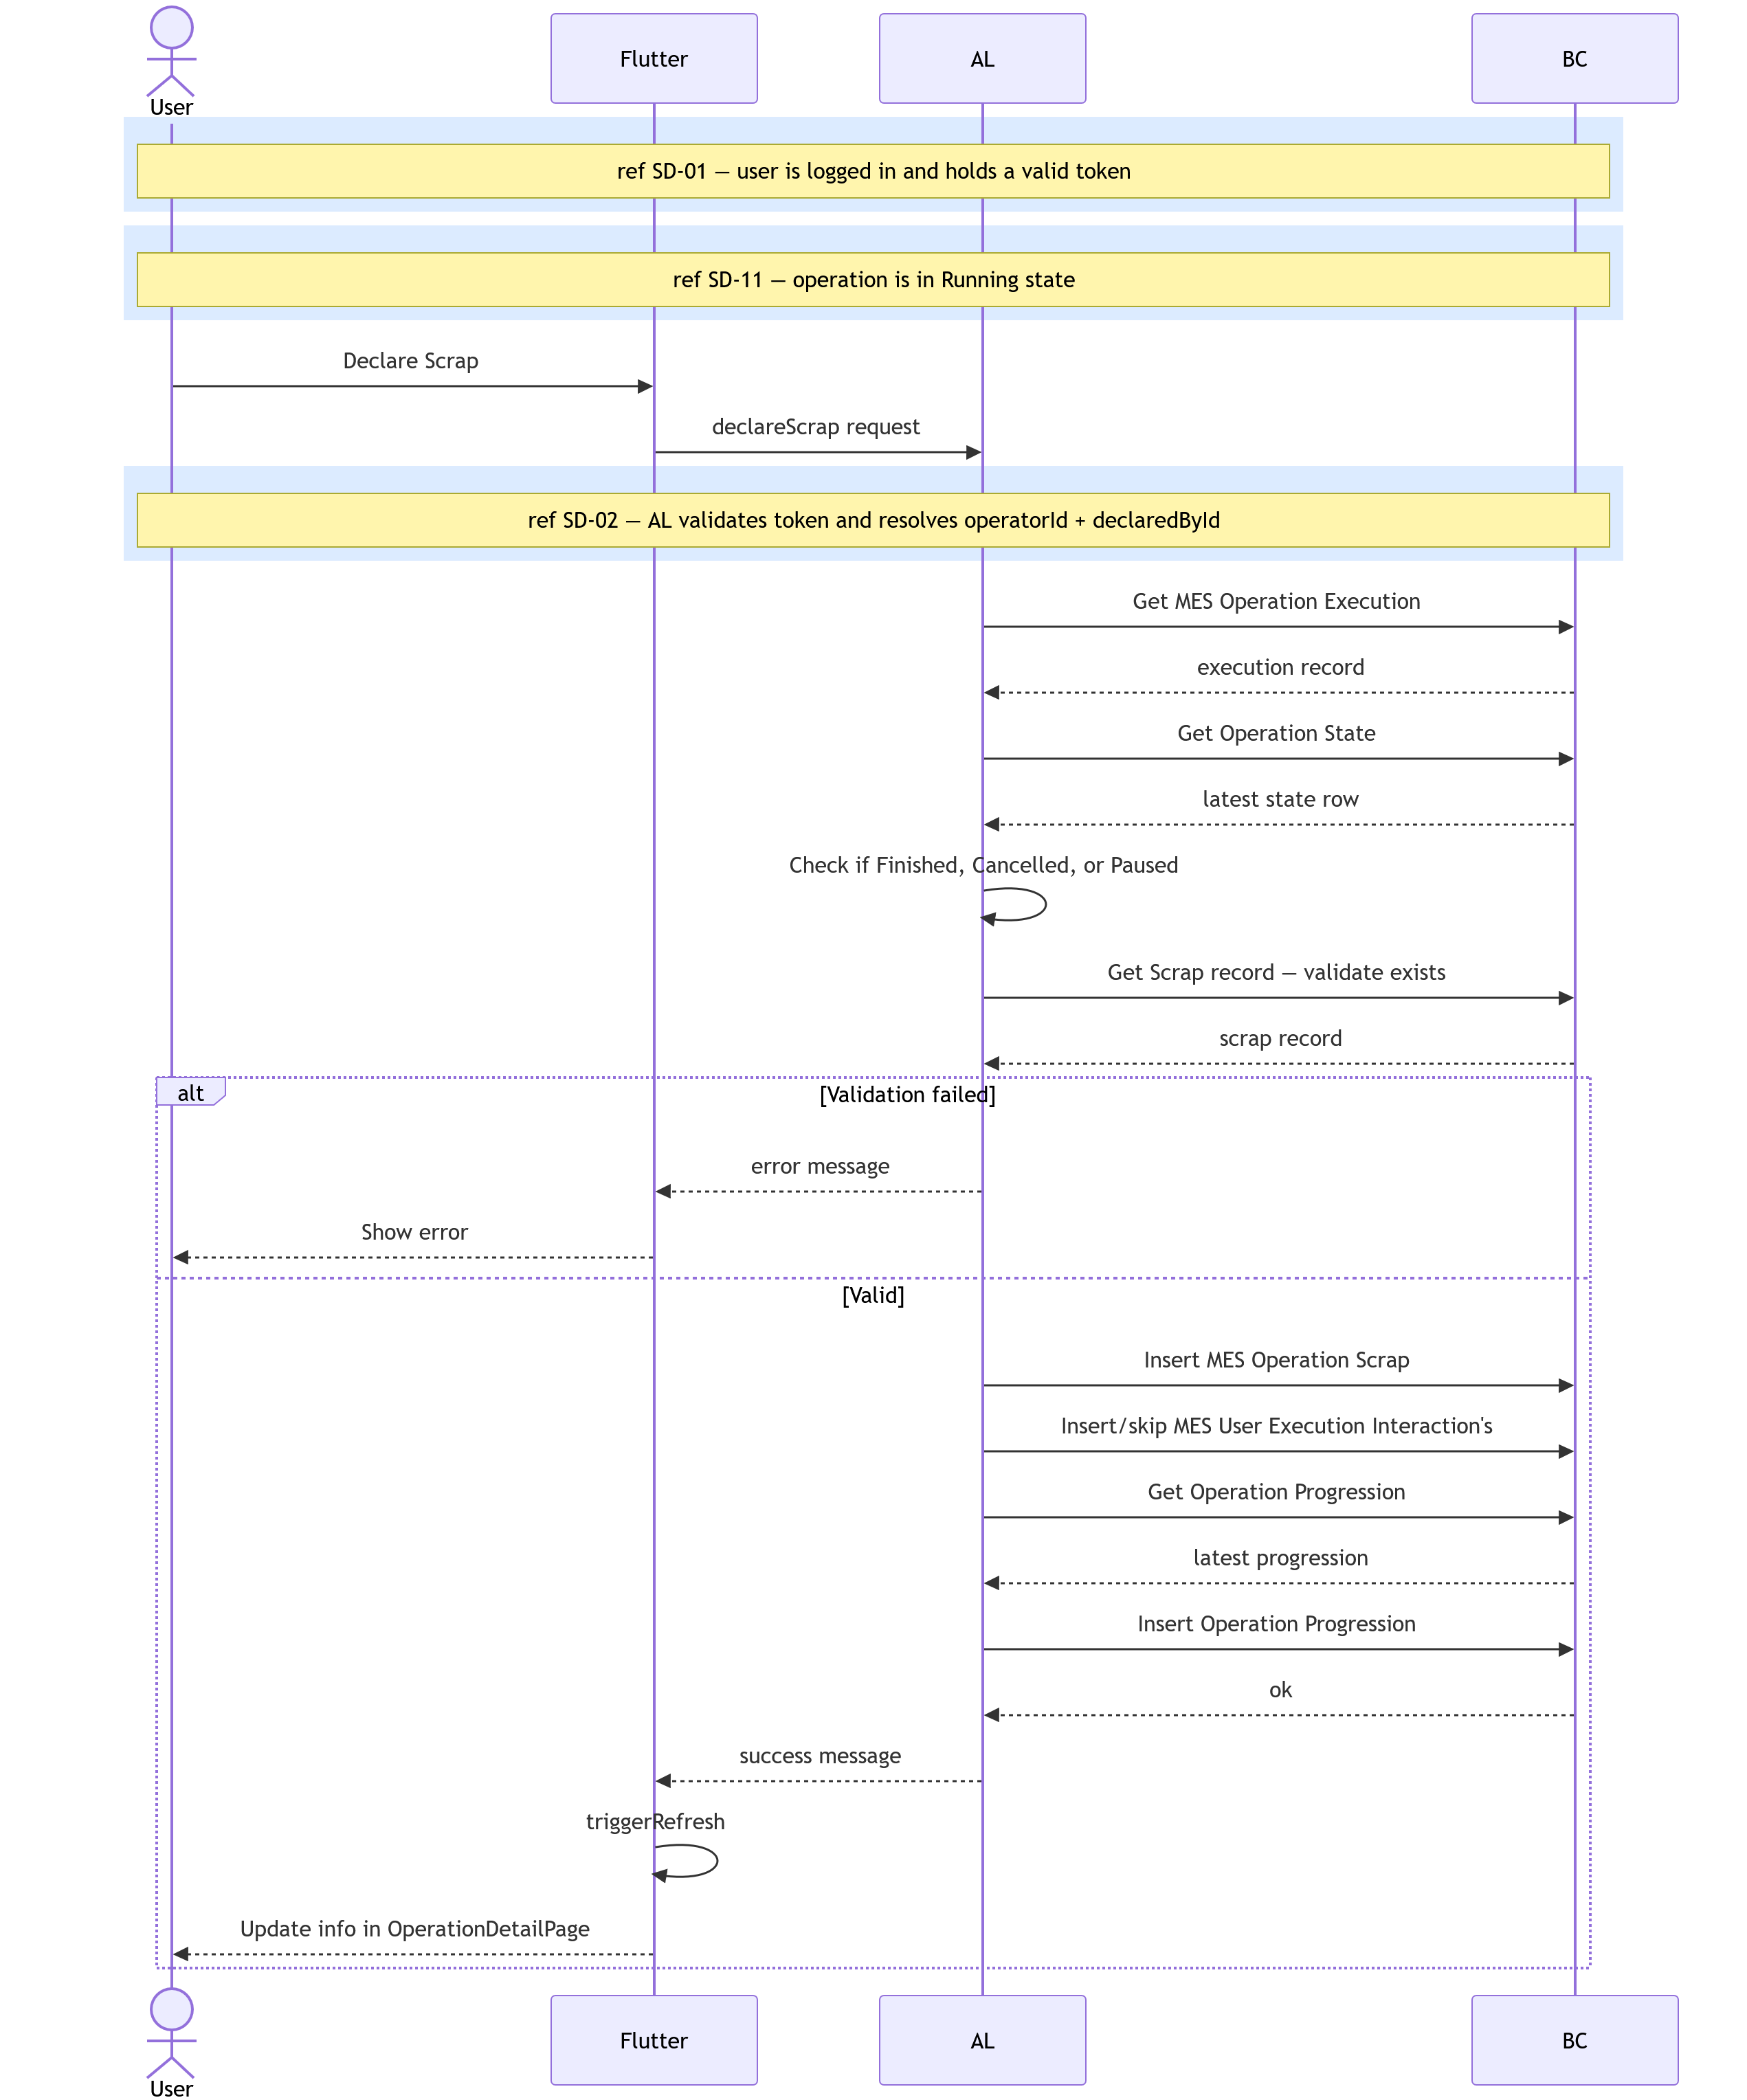
\includegraphics[width=\linewidth,height=0.82\textheight,keepaspectratio]{./media/MES_Sprint-3-Repport/diagrams/sequence/declare-scrap.png}
%   \caption{SD-16: declare scrap.}
%   \label{fig:s3-seq-declare-scrap}
% \end{figure}

%=====SD-16==========================================================
% sequenceDiagram
%     actor User
%     participant Flutter
%     participant Node as Node.js Middleware
%     participant AL
%     participant BC

%     rect rgb(220,235,255)
%         Note over User,BC: ref SD-01 — user is logged in and holds a valid token
%     end
%     rect rgb(220,235,255)
%         Note over User,BC: ref SD-11 — operation is in Running state, executionId known
%     end
%     User->>Flutter: fill out the scrap form
%     opt Material type
%         User->>Flutter: Select component from dropdown
%         Flutter->>Flutter: Set materialId = selectedComponent.itemNo
%     end
%     opt Supervisor declaring for operator
%         User->>Flutter: Select operator from OperatorSelector
%         Flutter->>Flutter: Set onBehalfOfUserId = selectedOperator.userId
%     end
%     User->>Flutter: Tap Submit
%     Flutter->>Node: POST /api/declareScrap
%     Node->>AL: MESWebService_declareScrap 

%       rect rgb(220,235,255)
%           Note over AL,BC: ref SD-02 — ValidateToken called
%       end

%       AL->>BC: get the execution record and the state of the operation
%       BC-->>AL: latest state ad execution record
%       AL->>BC: Validation
%       alt Validation failed
%           AL-->>Node: error response
%           Node-->>Flutter: error response
%           Flutter-->>User: Show error response
%       else Valid
%           AL->>BC: Insert MES Operation Scrap
%           BC-->>AL: ok
%           AL-->>Node: success response
%           Node-->>Flutter: success response
%           Flutter->>Flutter: refresh all the streams
%           Flutter-->>User: Updated scrap data visible in OperationDetailPage
%       end
%====================================================================

% Figure~\ref{fig:s3-seq-scan-component} illustrates the component scanning flow,
% which operates in two steps. First, the \techname{Flutter} client resolves
% each scanned barcode into an item record via a lightweight \texttt{resolveBarcode}
% call and accumulates the results locally. Once the operator confirms the
% batch, a single \texttt{insertScans} request is sent to the \techname{AL}
% layer, which inserts one \domainterm{MES Component Consumption} record per
% scanned item and records the associated user interaction entries.

% \begin{figure}[H]
%   \centering
%   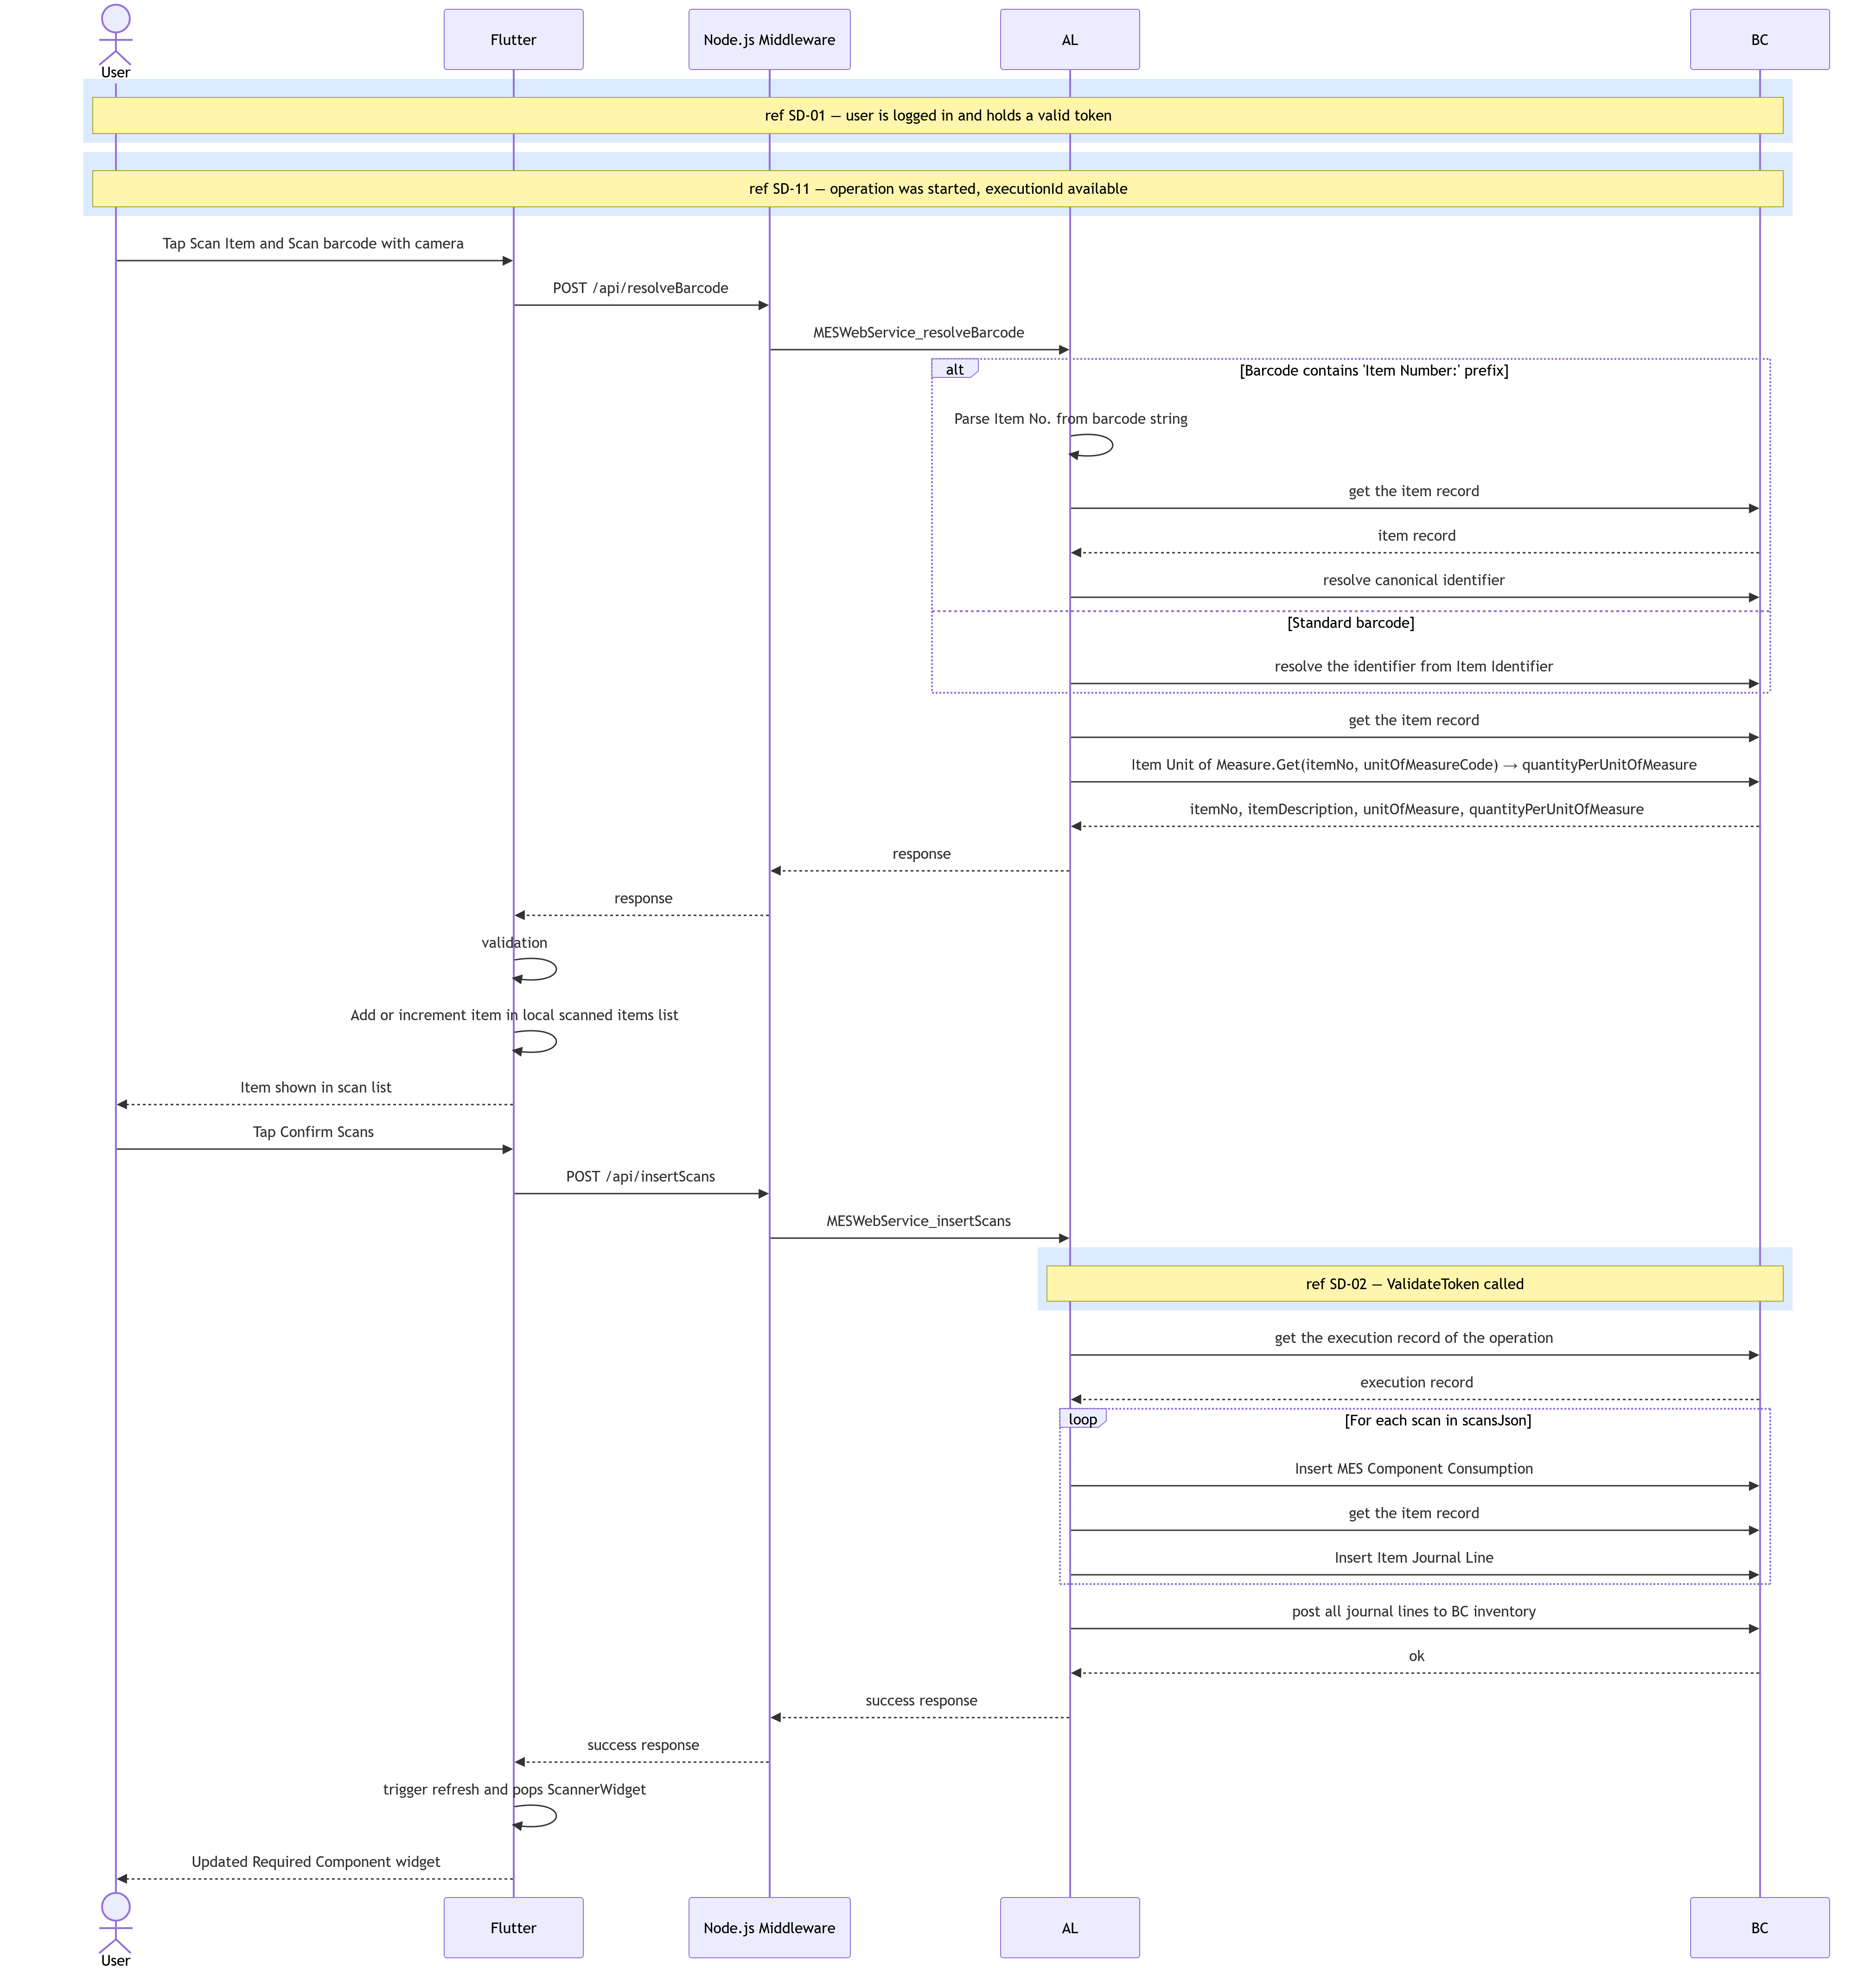
\includegraphics[width=\linewidth,height=0.82\textheight,keepaspectratio]{./media/MES_Sprint-3-Repport/diagrams/sequence/scan-component.png}
%   \caption{SD-17: scan component.}
%   \label{fig:s3-seq-scan-component}
% \end{figure}

%=====SD-17==========================================================
% sequenceDiagram
%       actor User
%       participant Flutter
%       participant Node as Node.js Middleware
%       participant AL
%       participant BC

%       rect rgb(220,235,255)
%           Note over User,BC: ref SD-01 — user is logged in and holds a valid token
%       end
%       rect rgb(220,235,255)
%           Note over User,BC: ref SD-11 — operation was started, executionId available
%       end

%       User->>Flutter: Tap Scan Item and Scan barcode with camera
%       Flutter->>Node: POST /api/resolveBarcode
%       Node->>AL: MESWebService_resolveBarcode

%       alt Barcode contains 'Item Number:' prefix 
%           AL->>AL: Parse Item No. from barcode string
%           AL->>BC: get the item record
%           BC-->>AL: item record 
%           AL->>BC: resolve canonical identifier
%       else Standard barcode
%           AL->>BC: resolve the identifier from Item Identifier
%       end
%       AL->>BC: get the item record
%       AL->>BC: Item Unit of Measure.Get(itemNo, unitOfMeasureCode) → quantityPerUnitOfMeasure
%       BC-->>AL: itemNo, itemDescription, unitOfMeasure, quantityPerUnitOfMeasure
%       AL-->>Node: response
%       Node-->>Flutter: response

%       Flutter->>Flutter: validation
%       Flutter->>Flutter: Add or increment item in local scanned items list
%       Flutter-->>User: Item shown in scan list

%       User->>Flutter: Tap Confirm Scans
%       Flutter->>Node: POST /api/insertScans 
%       Node->>AL: MESWebService_insertScans 

%       rect rgb(220,235,255)
%           Note over AL,BC: ref SD-02 — ValidateToken called
%       end

%       AL->>BC: get the execution record of the operation
%       BC-->>AL: execution record

%       loop For each scan in scansJson
%           AL->>BC: Insert MES Component Consumption 
%           AL->>BC: get the item record
%           AL->>BC: Insert Item Journal Line
%       end

%       AL->>BC: post all journal lines to BC inventory
%       BC-->>AL: ok
%       AL-->>Node: success response
%       Node-->>Flutter: success response
%       Flutter->>Flutter: trigger refresh and pops ScannerWidget
%       Flutter-->>User: Updated Required Component widget
%====================================================================

Figure~\ref{fig:s3-seq-fetch-operation-live-data} presents the live operation
data retrieval sequence. When the user navigates to the
\uilabel{OperationDetailPage}, three \techname{StreamBuilder} instances mount
simultaneously: one polling the current operation status and quantities from
\techname{Business Central} (SD-18), one consuming the production-cycle stream
(SD-22), and one consuming the BOM stream (SD-21). The \techname{Flutter}
client merges all three data sources and renders the full detail view. If the
operation is finished, cancelled, or not yet started, the live-data stream
returns an empty response and the client falls back to the history view.

\begin{figure}[H]
  \centering
  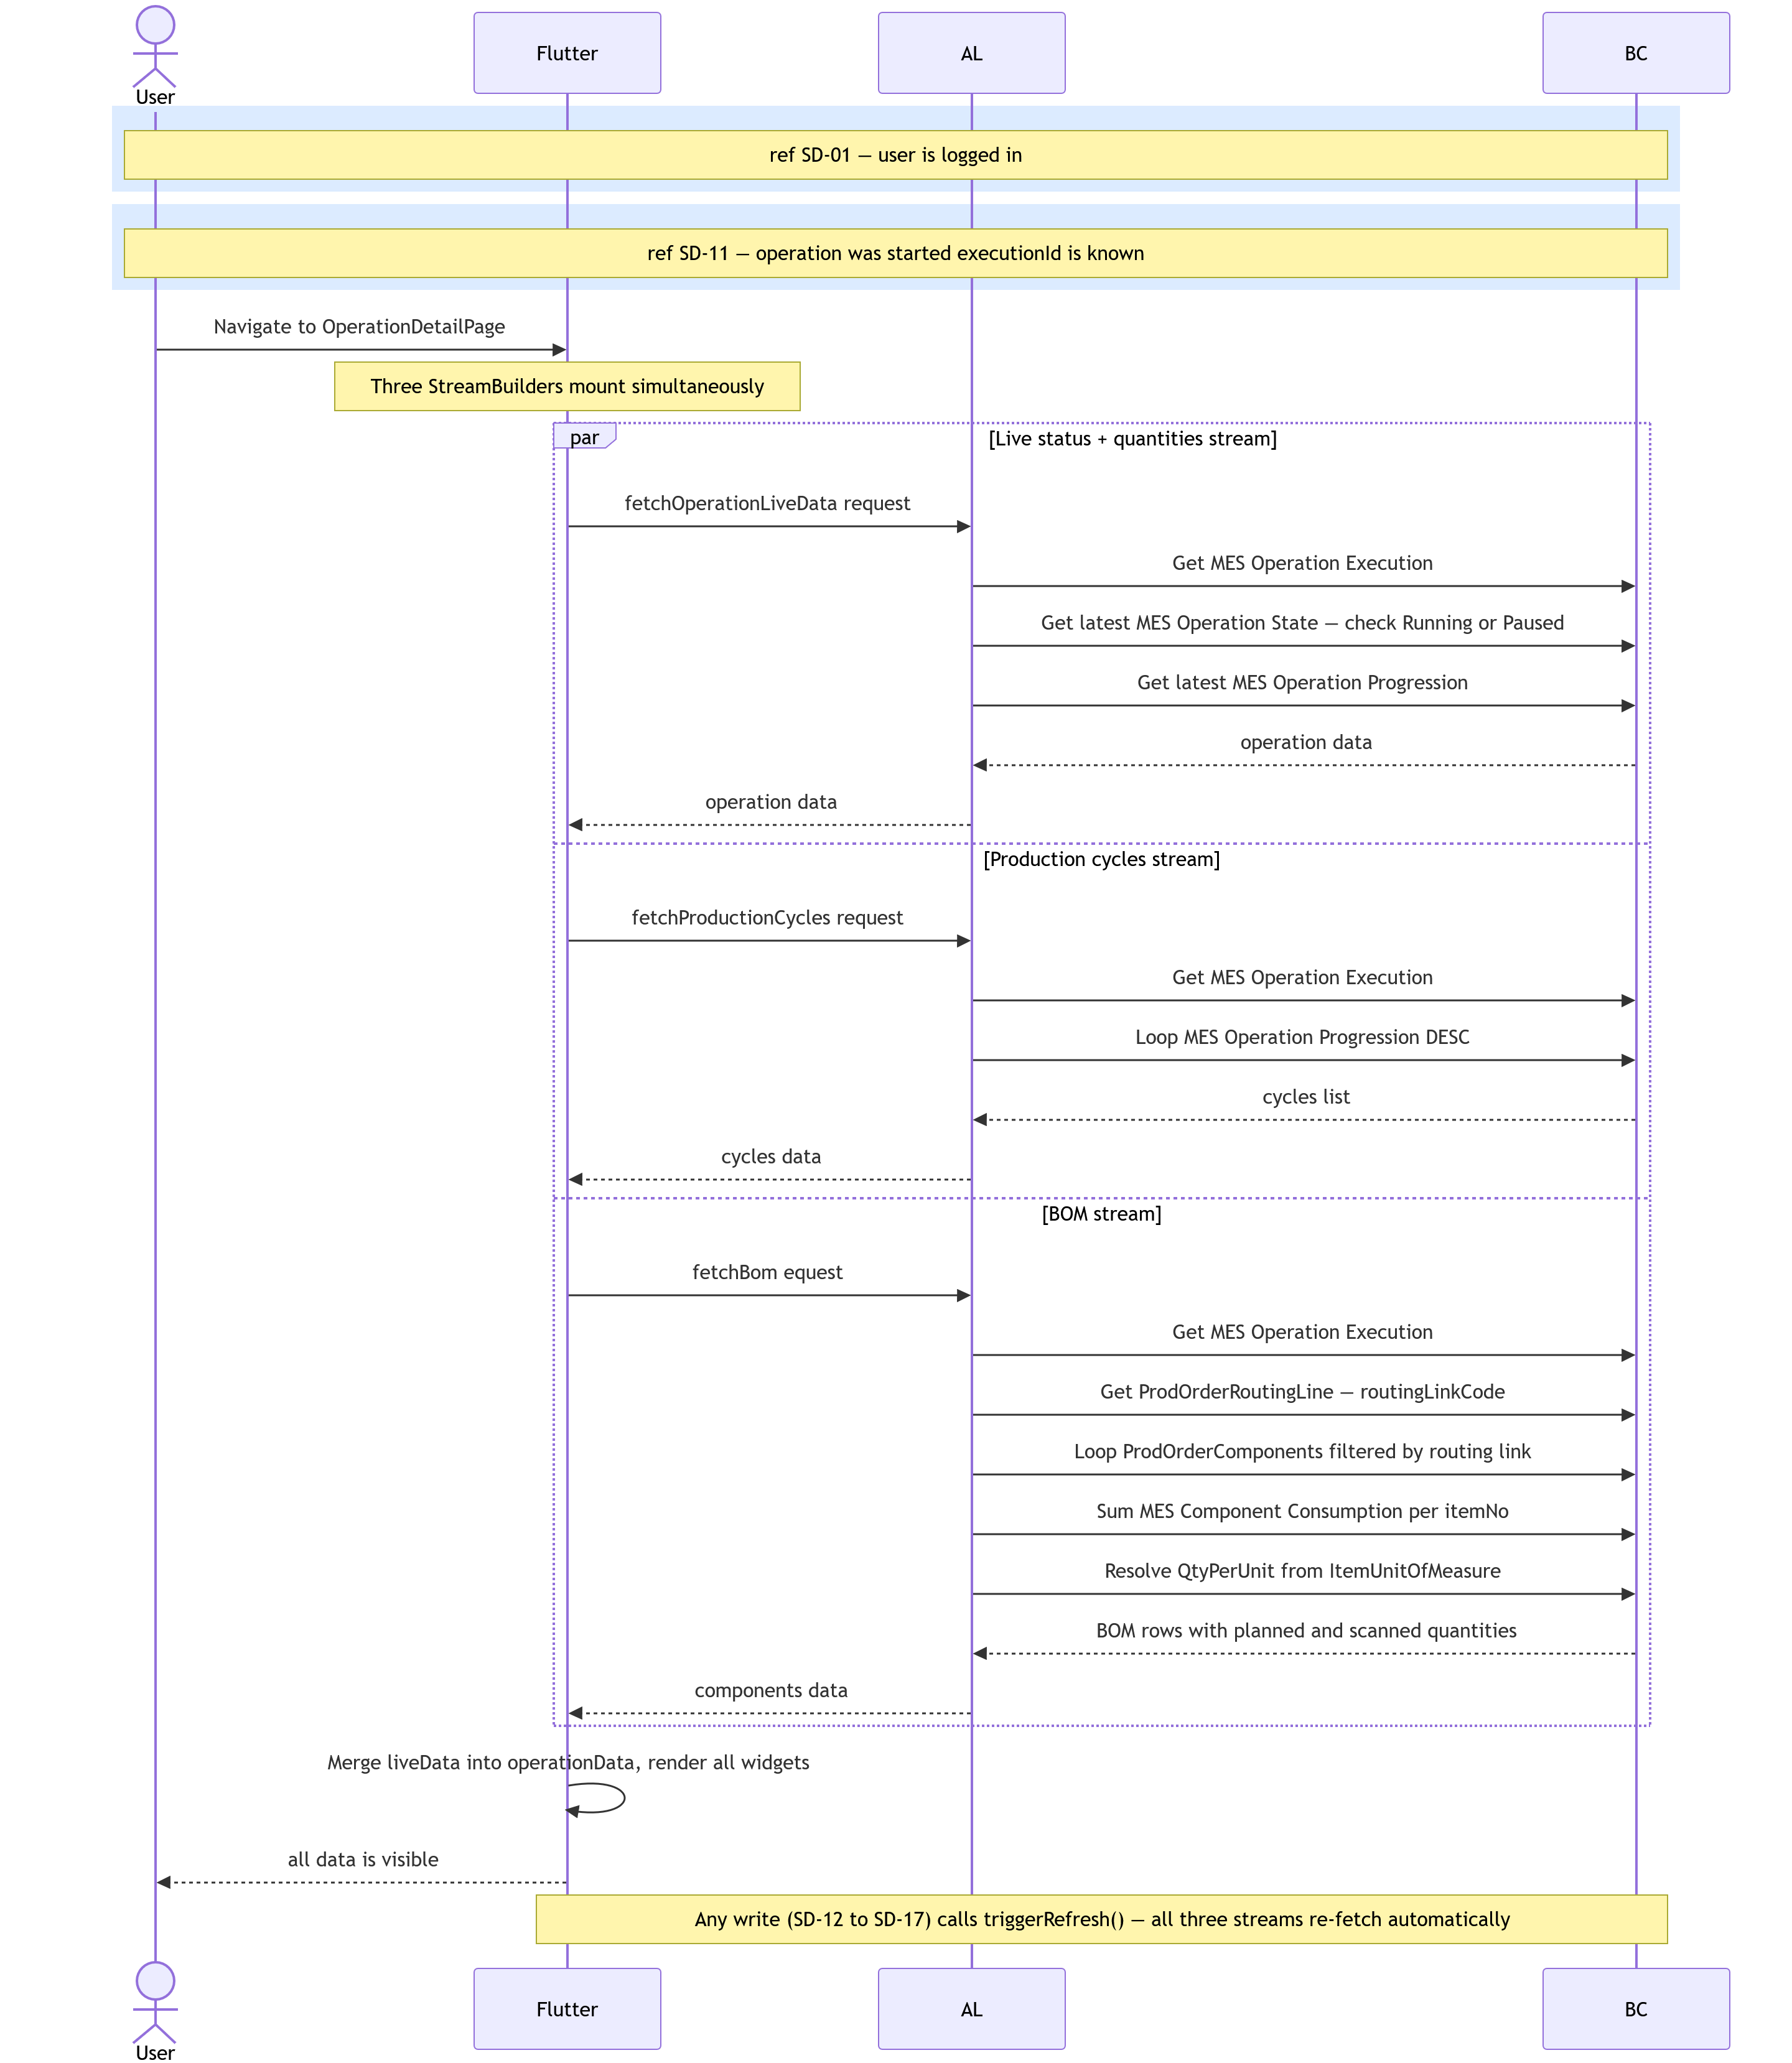
\includegraphics[width=\linewidth,height=0.82\textheight,keepaspectratio]{./media/MES_Sprint-3-Repport/diagrams/sequence/fetch-operation-live-data.png}
  \caption{SD-18: Fetch Operation Live Data.}
  \label{fig:s3-seq-fetch-operation-live-data}
\end{figure}

%=====SD-18==========================================================
%  sequenceDiagram
%       actor User
%       participant Flutter
%       participant Node as Node.js Middleware
%       participant AL
%       participant BC

%       rect rgb(220,235,255)
%           Note over User,BC: ref SD-01 — user is logged in
%       end
%       rect rgb(220,235,255)
%           Note over User,BC: ref SD-11 — operation was started, executionId known
%       end

%       User->>Flutter: Navigate to OperationDetailPage

%       par Live status + quantities stream (fetchOperationLiveData)
%           Flutter->>Node: POST /api/fetchOperationLiveData 
%           Node->>AL: MESWebService_fetchOperationLiveData 
%           AL->>BC: get the execution record and state of the operation
%           BC-->>AL: execution record and the current state of the operation
%           AL->>BC: resolve the scrap Qte
%           Note over AL,BC: Only finished-product scrap counted in live scrapQuantity
%           BC-->>AL: scrapQuantity sum
%           AL->>BC:get the operation progress
%           BC-->>AL: latest progression
%           AL-->>Node: live data JSON
%           Node-->>Flutter: live data
%       and Production cycles stream (ref SD-22)
%           Note over Flutter,BC: ref SD-22 — fetchProductionCycles stream
%       and BOM / components stream (ref SD-21)
%           Note over Flutter,BC: ref SD-21 — fetchBom stream
%       end

%       Flutter->>Flutter: Merge liveData fields into operationData record
%       Flutter-->>User: All data visible in OperationDetailPage
%====================================================================


\subsection{Class Diagram}

The UML Class Diagram (Figure~\ref{fig:s3-class-diagram-s3}) extends the Sprint~2
domain model with three new tables. \modulename{MES Operation Execution} (50110)
is the central anchor record linking a machine, production order, and operation
to its full lifecycle; it holds item description, order quantity, and start/end
timestamps. \modulename{MES Operation Progression} (50109) is an append-only
table of production cycle declarations, each referencing an execution and
accumulating \texttt{TotalProducedQuantity} from the previous cycle.
\modulename{MES Component Consumption} (50111) records scrap and barcode scan
events, also referencing an execution. Both progression and consumption records
are child tables of the execution record, forming a hub-and-spoke traceability
model.

\begin{figure}[H]
  \centering
  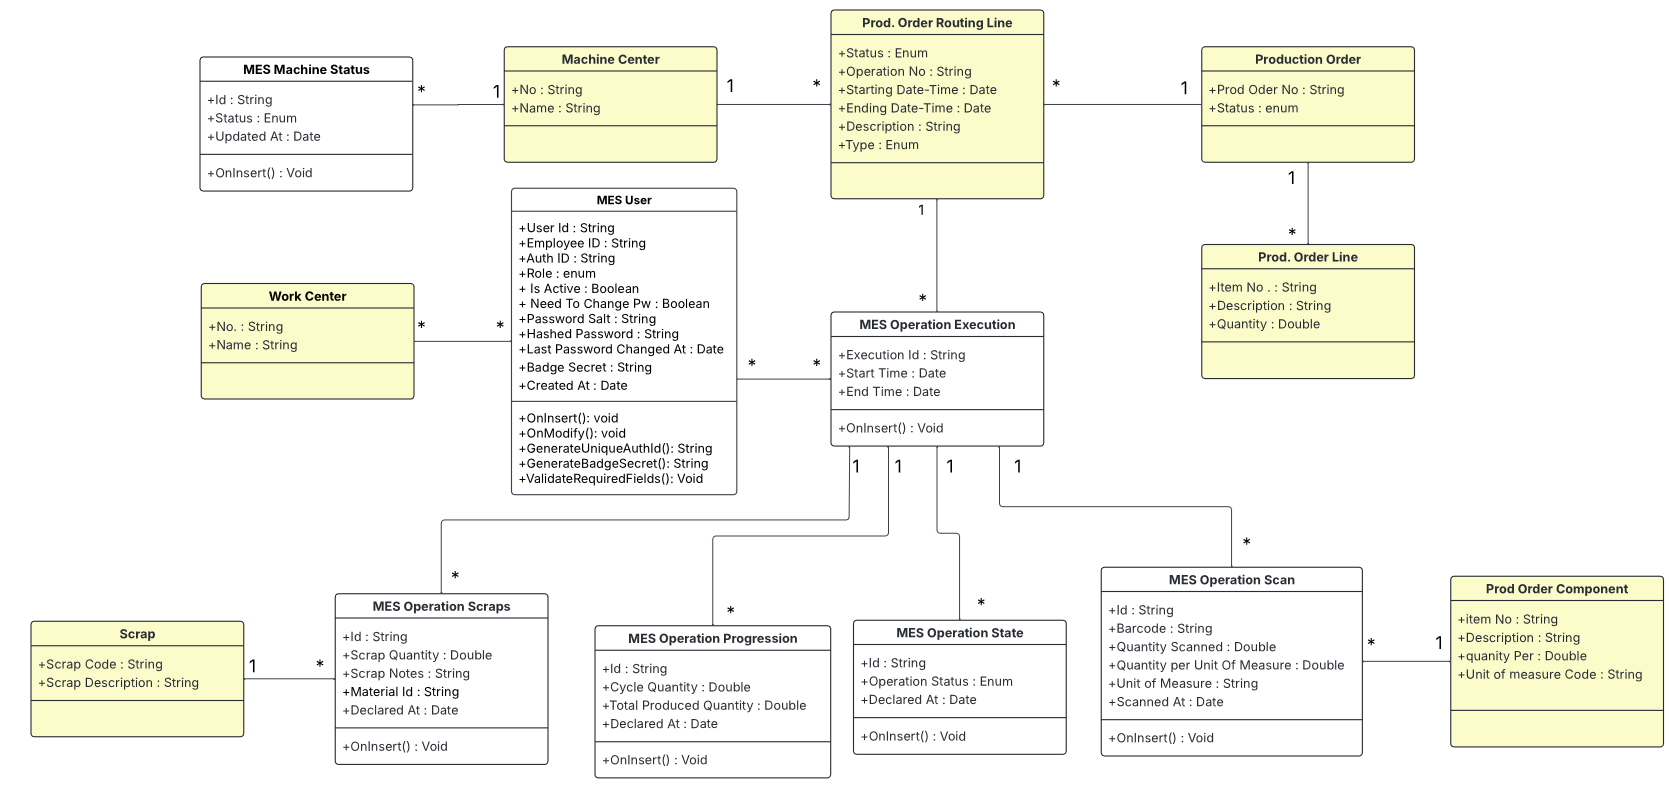
\includegraphics[width=\linewidth,keepaspectratio]{./media/MES_Sprint-3-Repport/diagrams/class/sprint3.png}
  \caption{UML Class Diagram --- Production Execution \& Traceability.}
  \label{fig:s3-class-diagram-s3}
\end{figure}

% ---------------------------------------------------------------------------
% 4. IMPLEMENTATION
% ---------------------------------------------------------------------------
\section{Implementation}

\subsection{Backend Implementation}
\subsubsection{Tables and Entities}

\begin{longtable}{@{} P{0.21\linewidth} P{0.17\linewidth} P{0.57\linewidth} @{}}
	\caption{MES Operation Execution (Table 50110) --- Field Dictionary}
	\label{tab:s3-table-execution} \\
	\toprule
	\textbf{Name} & \textbf{Type} & \textbf{Description} \\
	\midrule
	\endfirsthead
	\toprule
	\textbf{Name} & \textbf{Type} & \textbf{Description} \\
	\midrule
	\endhead
	
	\multicolumn{3}{r}{\small Continued on next page} \\
	\endfoot
	\bottomrule
	\endlastfoot
	
	Execution Id & Code[50] & GUID-based primary key; auto-generated on insert. \\
	\midrule
	Machine No & Code[20] & References Machine Center (no referential constraint enforced in the current implementation). \\
	\midrule
	Prod Order No & Code[20] & Foreign key to Prod.\ Order Routing Line. \\
	\midrule
	Operation No & Code[10] & Operation identifier from the routing line. \\
	\midrule
	Item No & Code[20] & Copied from Prod.\ Order Line on execution creation. \\
	\midrule
	Item Description & Text[100] & Copied from Prod.\ Order Line for denormalized display. \\
	\midrule
	Order Quantity & Decimal & Copied from Prod.\ Order Line; used for progress calculation. \\
	\midrule
	Start Time & DateTime & Set by \texttt{OnInsert} trigger to \texttt{CurrentDateTime()}. \\
	\midrule
	End Time & DateTime & Stamped when status transitions to Finished or Cancelled. \\
\end{longtable}

\begin{longtable}{@{} P{0.21\linewidth} P{0.17\linewidth} P{0.57\linewidth} @{}}
	\caption{MES Operation Progression (Table 50109) --- Field Dictionary}
	\label{tab:s3-table-progression} \\
	\toprule
	\textbf{Name} & \textbf{Type} & \textbf{Description} \\
	\midrule
	\endfirsthead
	\toprule
	\textbf{Name} & \textbf{Type} & \textbf{Description} \\
	\midrule
	\endhead
	\multicolumn{3}{r}{\small Continued on next page} \\
	\endfoot
	\bottomrule
	\endlastfoot
	
	Id & Code[50] & GUID-based primary key; auto-generated on insert. \\
	\midrule
	Execution Id & Code[50] & Foreign key to MES Operation Execution. \\
	\midrule
	Cycle Quantity & Decimal & Units declared in this single production cycle. \\
	\midrule
	Total Produced Quantity & Decimal & Running total: previous total + Cycle Quantity. \\
	\midrule
	Operator Id & Code[50] & BC session UserId of the user who produced the unites during this cycle. \\
	\midrule
	Declared At & DateTime & Set by \texttt{OnInsert} trigger to \texttt{CurrentDateTime()}. \\
	\midrule
	Declared By & Code[50] &  BC session UserId of the user who declared the production cycle  \\
\end{longtable}

\begin{longtable}{@{} P{0.21\linewidth} P{0.17\linewidth} P{0.57\linewidth} @{}}
	\caption{MES Operation Scan (Table 50111) --- Field Dictionary}
	\label{tab:s3-table-consumption} \\
	\toprule
	\textbf{Name} & \textbf{Type} & \textbf{Description} \\
	\midrule
	\endfirsthead
	\toprule
	\textbf{Name} & \textbf{Type} & \textbf{Description} \\
	\midrule
	\endhead
	\multicolumn{3}{r}{\small Continued on next page} \\
	\endfoot
	\endlastfoot
	
	Id & Code[50] & GUID-based primary key; auto-generated on insert. \\
	\midrule
	Execution Id & Code[50] & Foreign key to MES Operation Execution. \\
	\midrule
	Prod Order No & Code[50] & Foreign key to Prod.\ Order Component. \\
	\midrule
	Item No & Code[50] & Item identifier of the consumed component. \\
	\midrule
	Barcode & Text[500] & Barcode scanned to register the component. \\
	\midrule
	Unit of Measure & Code[50] & Unit of measure code from the component definition. \\
	\midrule
	Quantity Scanned & Decimal & Raw quantity read from the barcode scan. \\
	\midrule
	Quantity per Unit of Measure & Decimal & Unit-of-measure conversion factor; the effective consumed quantity equals Quantity Scanned multiplied by this value. \\	
	\midrule
	Operator Id & Code[50] & BC session UserId of the operator who scanned. \\
	\midrule
	Scanned At & DateTime & Set by \texttt{OnInsert} trigger to \texttt{CurrentDateTime()}. \\
	\midrule
	Declared By & Code[50] &  BC session UserId of the user who declared the production cycle  \\
	\midrule
\end{longtable}


\subsubsection{REST API and Web Services Implementation}

All endpoints are exposed as ODataV4 unbound actions through
\techname{MES Web Service} (codeunit~50126) and are served by the
middleware at:

\begin{center}
  \texttt{middlewareHostURL/api/<endpointName>}
\end{center}

\noindent Each request is forwarded to the \techname{AL} layer as an
ODataV4 action call of the form:

\begin{center}
  \texttt{POST~<baseUrl>/ODataV4/MESWebService\_<ProcedureName>?company=<companyId>}
\end{center}

\noindent Table~\ref{tab:s3-api-endpoints} lists all endpoints introduced
in this sprint.

\begin{longtable}{@{} P{0.48\linewidth} @{\hspace{0.04\linewidth}} P{0.48\linewidth} @{}}
  \caption{New API Endpoints --- Sprint 3}
  \label{tab:s3-api-endpoints}\\
  \toprule
  \textbf{Endpoint} & \textbf{Endpoint}\\
  \midrule
  \endfirsthead
  \toprule
  \textbf{Endpoint} & \textbf{Endpoint}\\
  \midrule
  \endhead
  \multicolumn{2}{r}{\small Continued on next page}\\
  \endfoot
  \bottomrule
  \endlastfoot

  \apiendpoint{startOperation}         & \apiendpoint{fetchOperationsStatusAndProgress} \\
  \midrule
  \apiendpoint{declareProduction}      & \apiendpoint{fetchOperationLiveData}            \\
  \midrule
  \apiendpoint{pauseOperation}         & \apiendpoint{fetchProductionCycles}             \\
  \midrule
  \apiendpoint{resumeOperation}        & \apiendpoint{fetchBom}                          \\
  \midrule
  \apiendpoint{finishOperation}        &                                                  \\
  \midrule
  \apiendpoint{cancelOperation}        &                                                  \\
\end{longtable}
\subsection{Frontend Implementation}

This sprint introduces a reactive pattern: a shared \texttt{StreamController<void>.broadcast()}
in \techname{MachineOrdersProvider} and \techname{MesComponentConsumptionProvider}. When any write
action (declare, pause, resume, finish, cancel) succeeds, \texttt{triggerRefresh()} adds an event 
to the controller. All live data streams (\texttt{fetchOperationLiveDataStream}, 
\texttt{streamProductionCycles}, \texttt{streamBom}) are implemented as \texttt{async*} generators
that yield on both the initial fetch and on each event from the shared broadcast stream, enabling 
coordinated, push-driven UI updates without polling.

\subsubsection{Provider Architecture}

\begin{longtable}{@{} P{0.30\linewidth} P{0.65\linewidth} @{}}
	\caption{Provider Responsibilities --- Sprint 3 Additions}
	\label{tab:s3-providers}\\
	\toprule
	\textbf{Provider}& \textbf{Responsibility}\\
	\midrule
	\endfirsthead
	\toprule
	\textbf{Provider}& \textbf{Responsibility}\\
	\midrule
	\endhead
	\multicolumn{2}{r}{\small Continued on next page}\\
	\endfoot
	\bottomrule
	\endlastfoot
	
	\techname{MachineOrdersProvider} & Owns write operations (start, declare, pause, resume, finish, cancel) and their refresh controller; exposes all live data streams. \\
	\midrule
	\techname{MesComponentConsumption\allowbreak Provider} & Exposes \texttt{getBomStream()} combining service fetch with an independent refresh controller.\\
	\midrule
	\techname{AuthProvider}& Adds \texttt{changePassword()} and \texttt{adminSetPassword()}; manages \texttt{needsPasswordChange} flag in the in-memory session. \\
\end{longtable}

\subsubsection{User Interface}
Figures~\ref{fig:s3-ui-op-detail-running} through~\ref{fig:s3-ui-op-detail-cancelled} illustrate the \uilabel{Operation Detail Page}
across its five possible states: Running, Paused, Finished, Interrupted, and Cancelled. Each view adapts its action buttons and status badge
to the current state, while the production chart, cycle table, and BOM list remain consistently visible. On desktop, the page 
uses a two-column layout with order information and production data on the left, and the \uilabel{Quick Actions} panel on the
right; on mobile, these sections stack vertically. Action button availability is state-dependent: \uilabel{Declare Production} 
and \uilabel{Declare Scrap} are disabled in the Paused, Finished, and Cancelled states; the close button triggers a 
\uilabel{Finish Production Order} or \uilabel{Interrupt Production Order} action depending on whether the progress has reached 100\%;
and \uilabel{Print Label} is enabled only once the operation is finished.

\begin{figure}[H]
    \centering
    \setlength{\fboxsep}{5pt}
    \colorbox{black}{%
        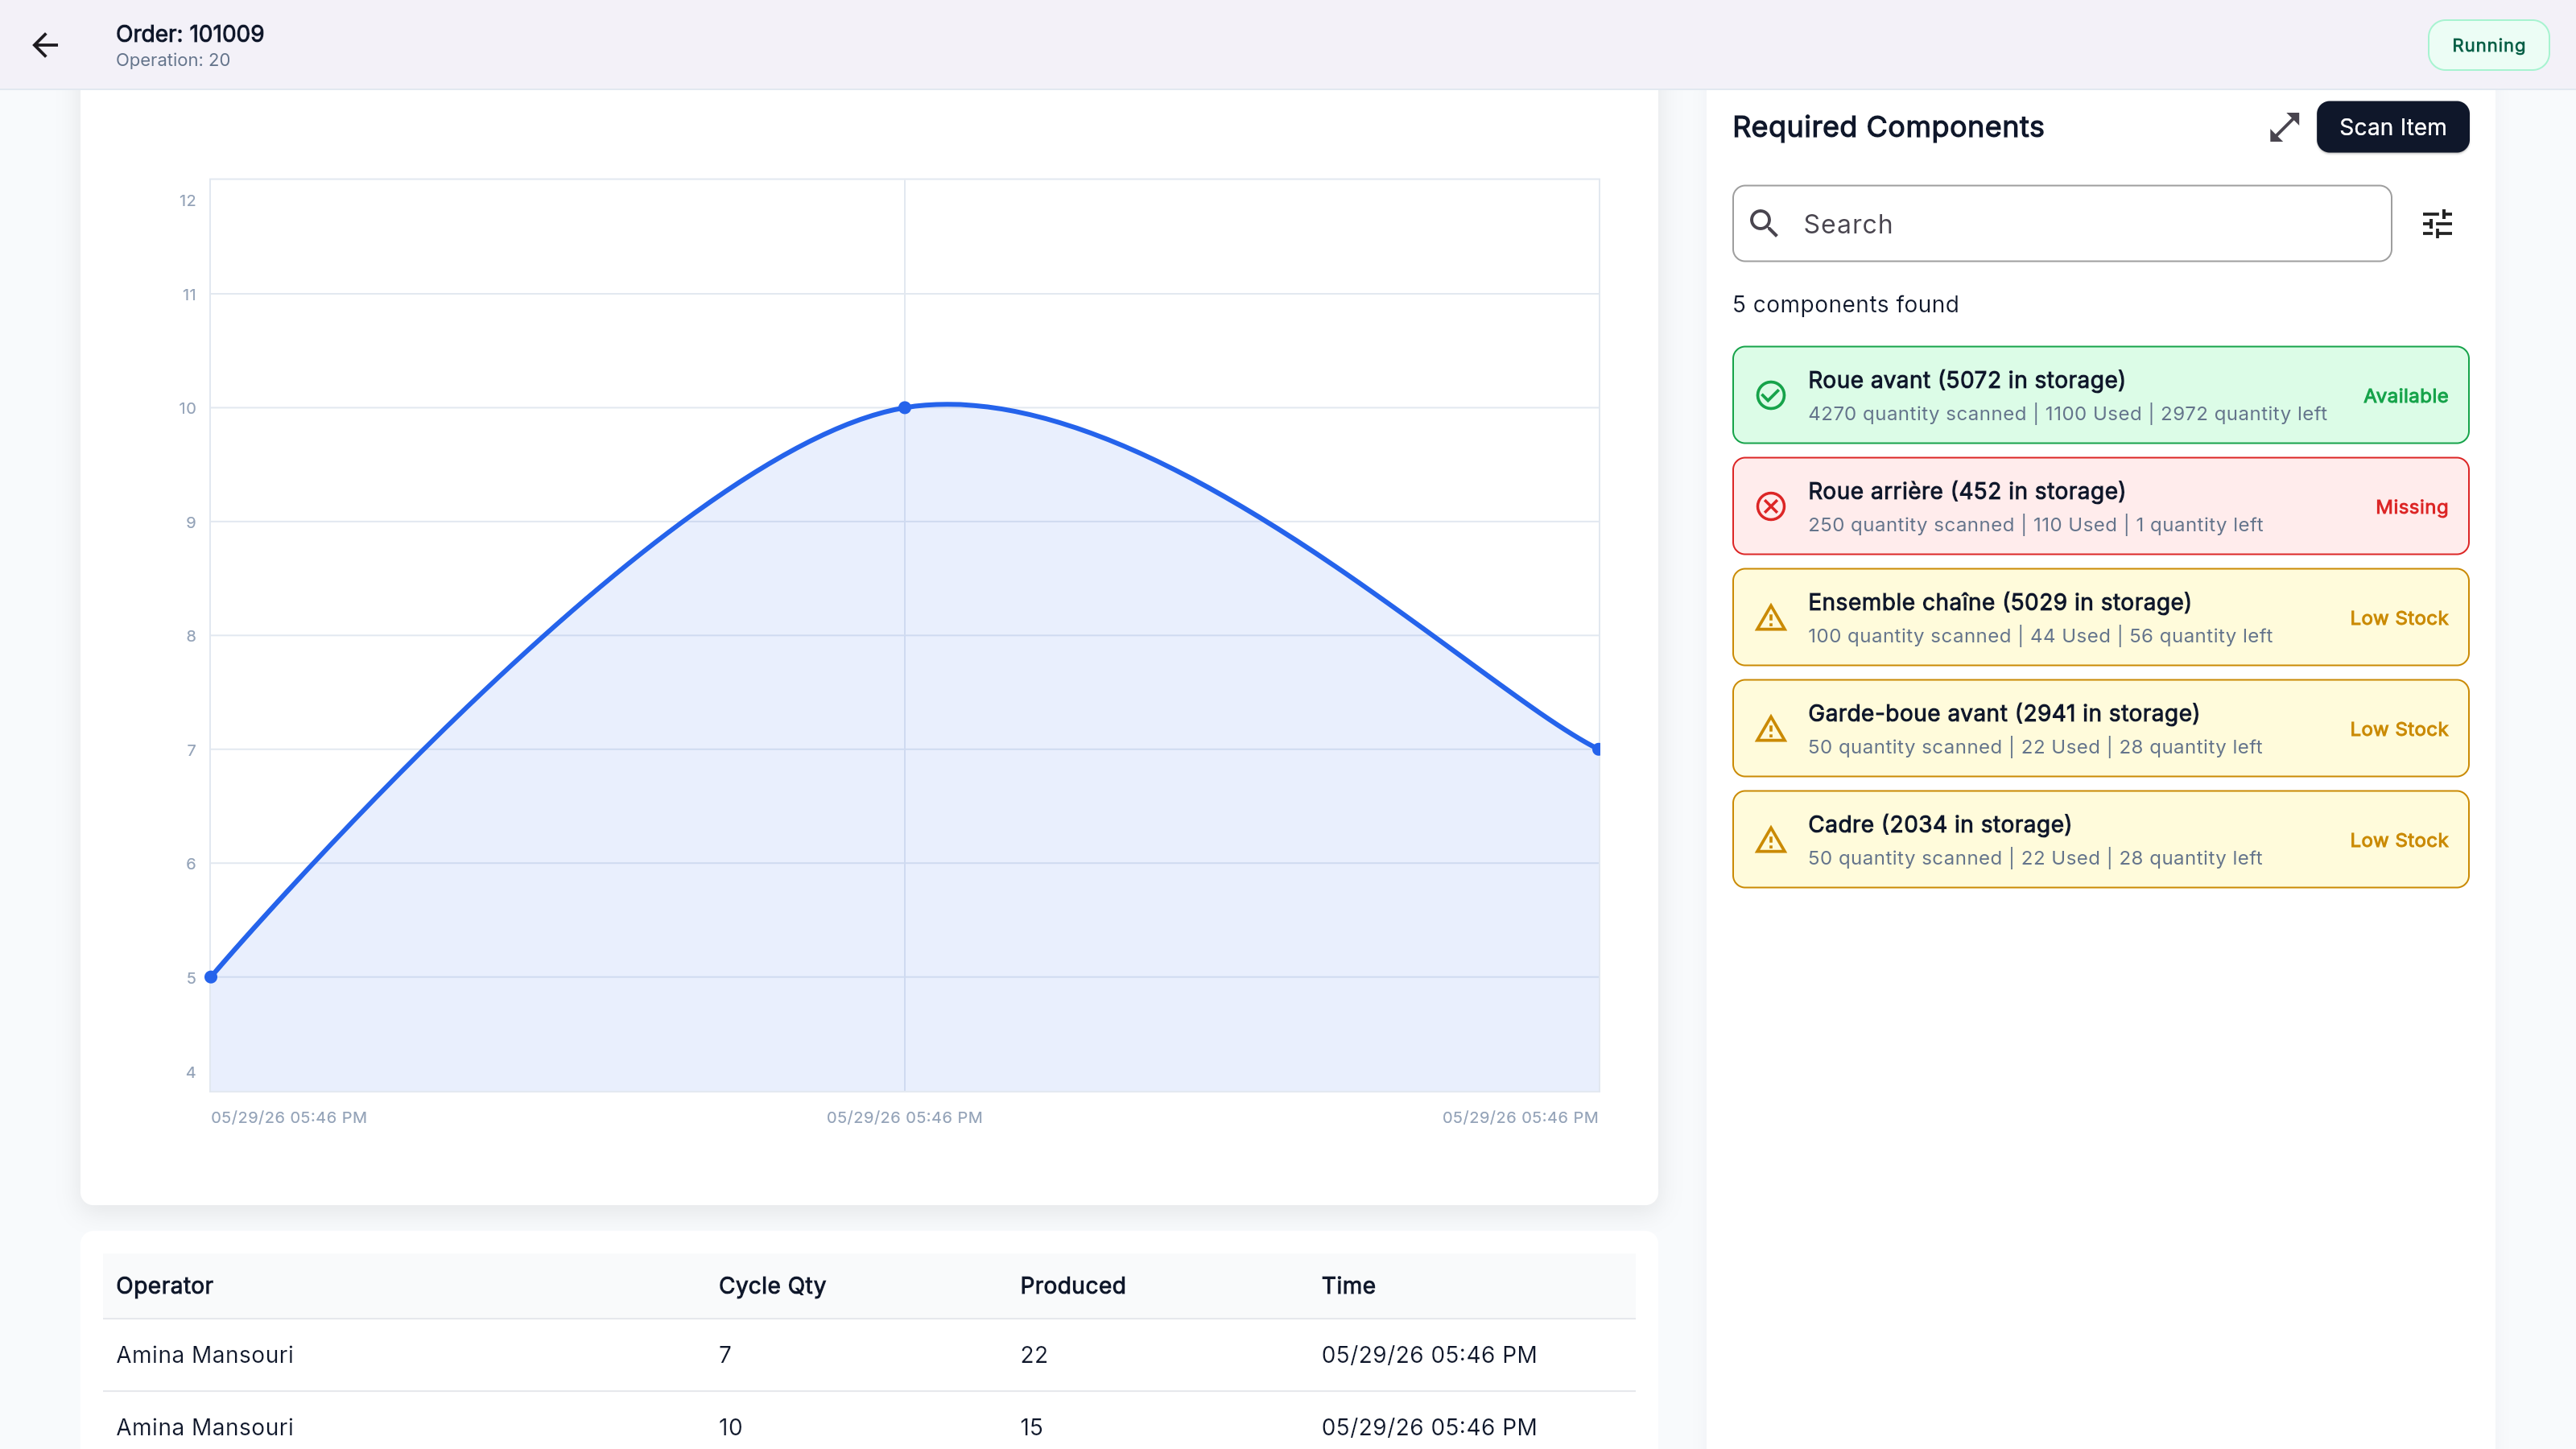
\includegraphics[height=0.3\textheight,keepaspectratio]{./media/MES_Sprint-3-Repport/UI/opDetailRunning/wide.png}%
        \hspace{\fboxsep}%
        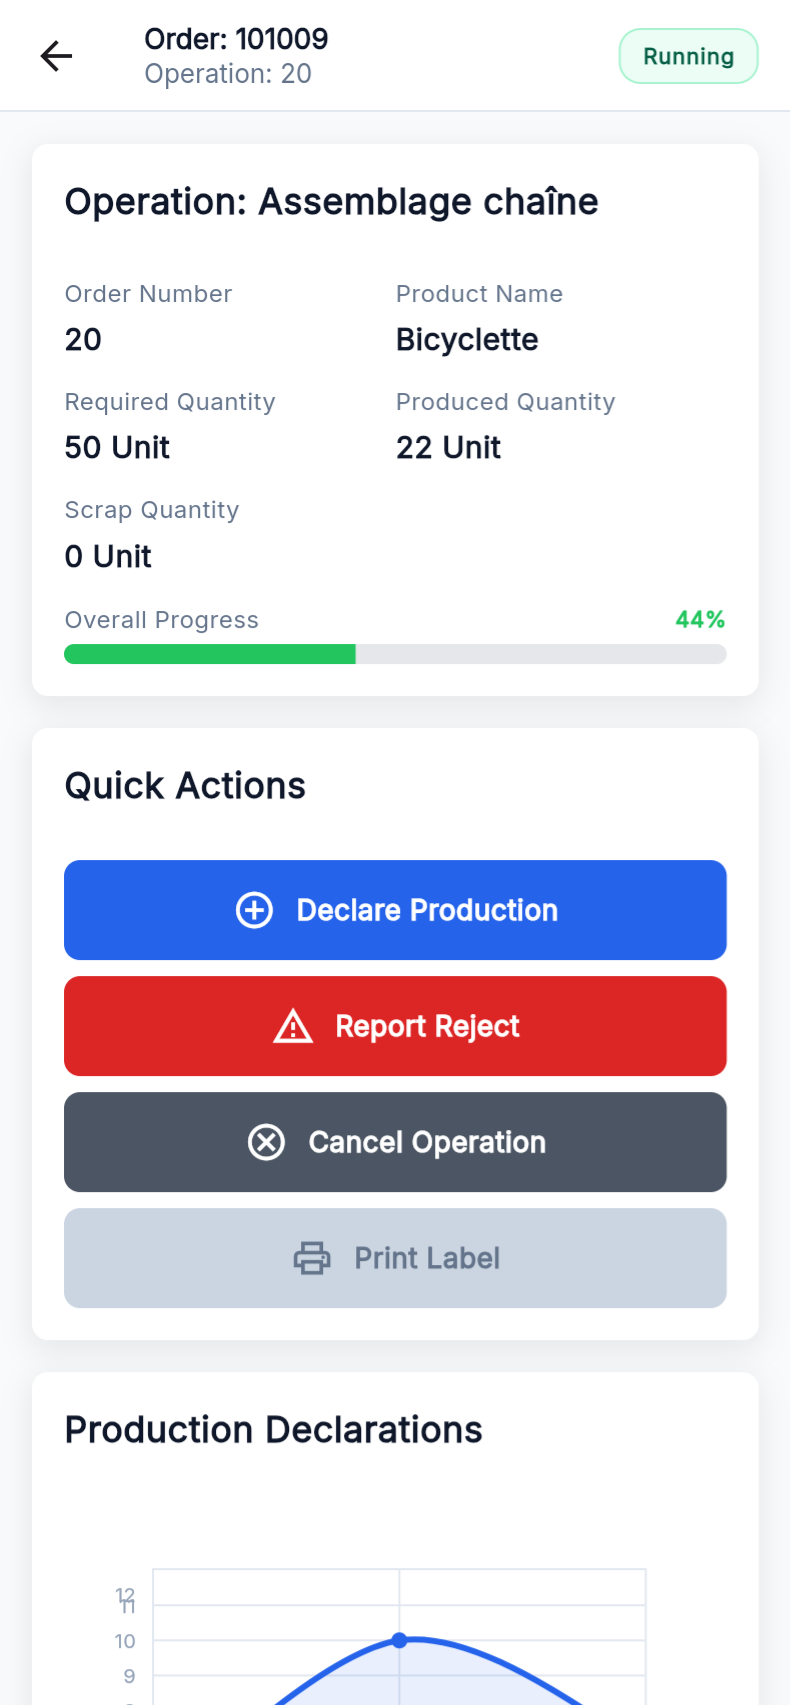
\includegraphics[height=0.3\textheight,keepaspectratio]{./media/MES_Sprint-3-Repport/UI/opDetailRunning/small.png}%
    }
    \caption{\uilabel{Operation Detail Page} (Running state) --- desktop and mobile views.}
    \label{fig:s3-ui-op-detail-running}
\end{figure}


\begin{figure}[H]
	\centering
	\setlength{\fboxsep}{5pt}
	\colorbox{black}{%
		
\includegraphics[height=0.3\textheight,keepaspectratio]{./media/MES_Sprint-3-Repport/placeholder-image.png}%
		\hspace{\fboxsep}%
		
\includegraphics[height=0.3\textheight,keepaspectratio]{./media/MES_Sprint-3-Repport/placeholder-image.png}%
	}
	\caption{\uilabel{Operation Detail Page} (Cancelled state) --- desktop and mobile views.}
	\label{fig:s3-ui-op-detail-cancelled}
\end{figure}

\section{Test and Validation}
\subsection{Integration test}

For integration testing, we chose Postman, a powerful and user-friendly tool for API evaluation. Figure~\ref{fig:s3-test-postman-fetchBom} shows a test case for the \apiendpoint{/fetchBom} endpoint.

\begin{figure}[H]
  \centering
  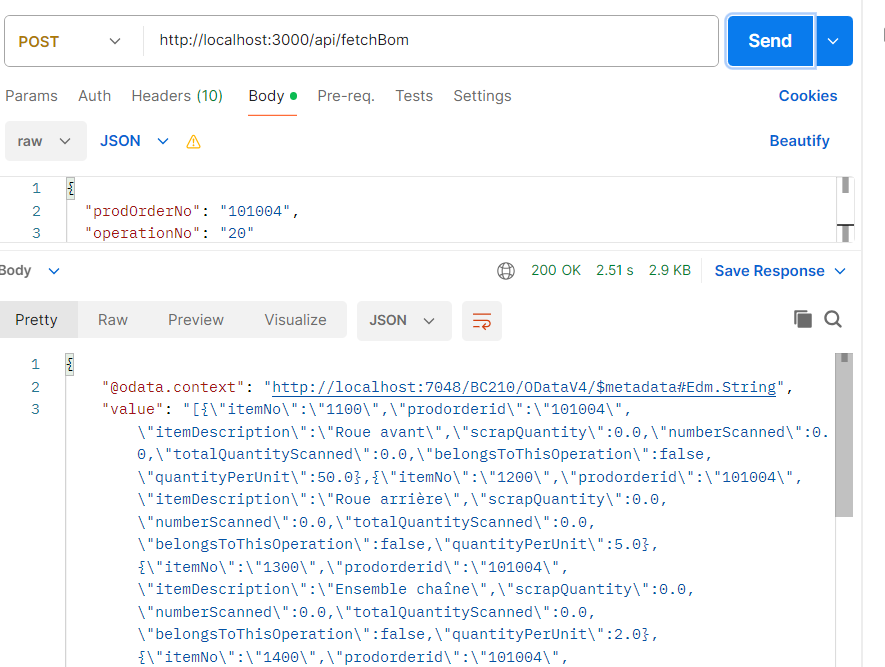
\includegraphics[width=\linewidth,keepaspectratio]{./media/MES_Sprint-3-Repport/test/postman/fetchBom.png}
  \caption{Postman endpoint test --- fetchBom.}
  \label{fig:s3-test-postman-fetchBom}
\end{figure}

\phantomsection
\section*{Conclusion}
\addcontentsline{toc}{section}{Conclusion}

This sprint delivered the complete shop-floor execution loop for the MES system.
Operators can now start, pause, resume, interrupt and close production operations, declare
production output cycle by cycle, track cumulative progress through real-time
charts and paginated tables, inspect the Bill of Materials, scan physical components
via barcodes, declare scrapped units with reason codes, and print
traceable labels for both production orders and individual declared units.
Supervisors gain the ability to declare production on behalf of a specific operator,
with a full attribution audit trail. The reactive stream architecture ensures that
all UI panels update in concert after every write action, providing a consistent
and accurate view of the production floor without manual refreshes.


% ---------------------------------------------------------------------------
% Sprint 4 Administration \& System Monitoring
% ---------------------------------------------------------------------------
\chapter{Sprint 4 Administration \& System Monitoring}
\graphicspath{{./media/MES_Sprint-4-Report/}}
\minitoc
\newpage
\section*{Introduction}
\addcontentsline{toc}{section}{Introduction}

This sprint delivers the administration layer, multi-language support, and
in-app onboarding tutorials that complete the \domainterm{MES} solution.
Administrators receives access to an activity log, and a user role management
interface. Quality-of-life features include full internationalisation with English,
French, and Arabic support, automatic right-to-left layout for Arabic, and guided 
coach-mark tutorials shown once in the main screens on first use. This sprint also 
delivers machine performance dashboard for the \userrole{Supervisor}. No new
\techname{Business Central} tables are introduced in this sprint; all data is
derived by querying and aggregating the tables created in Sprints~1 through~3.

% ---------------------------------------------------------------------------
% 1. SPRINT BACKLOG
% ---------------------------------------------------------------------------
\section{Sprint Backlog}

This sprint covers \textbf{Domain 4:}
\textbf{\domainterm{Administration \& Monitoring}}

% ----------------------------------------------------------
%  US-4.1
% ----------------------------------------------------------
\begin{longtable}{@{} P{0.09\linewidth} P{0.34\linewidth} P{0.53\linewidth} @{}}
      \caption{Sprint 4 Story Backlog}
      \label{tab:s4-sprint-backlog} \\
      \toprule
      \textbf{ID} & \textbf{User Story} & \textbf{Tasks} \\
      \midrule
      \endfirsthead
      \toprule
      \textbf{ID} & \textbf{User Story} & \textbf{Tasks} \\
      \midrule
      \endhead
      \multicolumn{3}{r}{\small Continued on next page} \\
      \endfoot
      \bottomrule
      \endlastfoot
            
      \textbf{US-4.1}
      & As an \userrole{Supervisor}, I need a performance dashboard for all
      machines so that I can monitor production health across the facility.
      & \noindent\textit{Business Central (AL):}
      \begin{itemize}[noitemsep, topsep=0pt, partopsep=0pt, leftmargin=*]
            \item Create function \texttt{fetchMachineDashboard()} in codeunit \techname{MES Machine Fetch}.
            \item Expose the function through the codeunit \techname{MES Web Service}.
      \end{itemize}
      \\ & &
      \noindent\textit{Flutter:}
      \begin{itemize}[noitemsep, topsep=0pt, partopsep=0pt, leftmargin=*]
            \item Create model \techname{MachineDashboardModel}.
            \item Create \techname{LogService} to consume the \texttt{fetchMachineDashboard} API and \techname{LogProvider} to manage its state.
            \item Create page \techname{MachineDashboardPage}.
            \item Implement machine dashboard search and time-range filtering in \techname{MachineDashboardPage}.
      \end{itemize} \\  
      \midrule 
      \textbf{US-4.2}
      & As an \userrole{Administrator}, I need a filterable log of all
      system actions so that I can audit operator and machine activity.
      & \noindent\textit{Business Central (AL):}
      \begin{itemize}[noitemsep, topsep=0pt, partopsep=0pt, leftmargin=*]
            \item Create function \texttt{fetchActivityLog()} in codeunit \techname{MES Machine Fetch}.
            \item Add the wrapper of the function to \techname{MES Web Service}.
      \end{itemize}
      \\ & &
      \noindent\textit{Flutter:}
      \begin{itemize}[noitemsep, topsep=0pt, partopsep=0pt, leftmargin=*]
            \item Create model \techname{ActivityLogModel}.
            \item Create \techname{LogService} to consume the \texttt{fetchActivityLog()} API and \techname{LogProvider} to manage its state.
            \item Create page \techname{ActivityLogPage}.
            \item Implement activity log search, type filtering, time-range filtering, and pagination in \techname{ActivityLogPage}.
      \end{itemize} \\
      \midrule
      \textbf{US-4.3}
      & As any user, I need the application available in English, French, and
      Arabic so that I can use it in my preferred language.
      & \noindent\textit{Flutter:}
      \begin{itemize}[noitemsep, topsep=0pt, partopsep=0pt, leftmargin=*]
            \item Integrate the \texttt{easy\_localization} package.
            \item Create translation JSON files for \texttt{en}, \texttt{fr}, and \texttt{ar}.
            \item Create widget \techname{LanguageSelector}.
            \item Implement language selection in \techname{ProfilePage}.
            \item Add the \techname{EasyLocalization} wrapper in \texttt{main()}.
            \item Implement right-to-left layout support through \texttt{MaterialApp}.
      \end{itemize} \\
      \midrule
      \textbf{US-4.4}
      & As a first-time user, I need guided coach-mark tutorials so that I can
      learn the interface without external documentation.
      & \noindent\textit{Flutter:}
      \begin{itemize}[noitemsep, topsep=0pt, partopsep=0pt, leftmargin=*]
            \item Integrate the \texttt{tutorial\_coach\_mark} package.
            \item Implement tutorial persistence using \techname{SharedPreferences}.
            \item Create \techname{MachineListTutorial}, \techname{MachineDetailTabsTutorial}, \techname{OperationDetailTutorial}, and \techname{AdminDashboardTutorial}.
            \item Implement tutorial target styling and localisation.
      \end{itemize} \\
\end{longtable}
% ---------------------------------------------------------------------------
% 2. BUSINESS RULES
% ---------------------------------------------------------------------------
\section{Design}

\subsection{Use Case Diagram}

The UML Use Case Diagram (Figure~\ref{fig:s4-use-case-s4}) covers the actors and
interactions introduced in this sprint. The \userrole{Administrator} gains the
interaction \uilabel{View Activity Log}.The \userrole{Supervisor} gains the interaction
\uilabel{View Machine Dashboard}. All three actors (\userrole{Operator},
\userrole{Supervisor}, \userrole{Administrator}) share the
\uilabel{Select Language} and \uilabel{View Tutorial} use cases, which are
cross-cutting accessibility features available on every screen.

\begin{figure}[H]
      \centering
      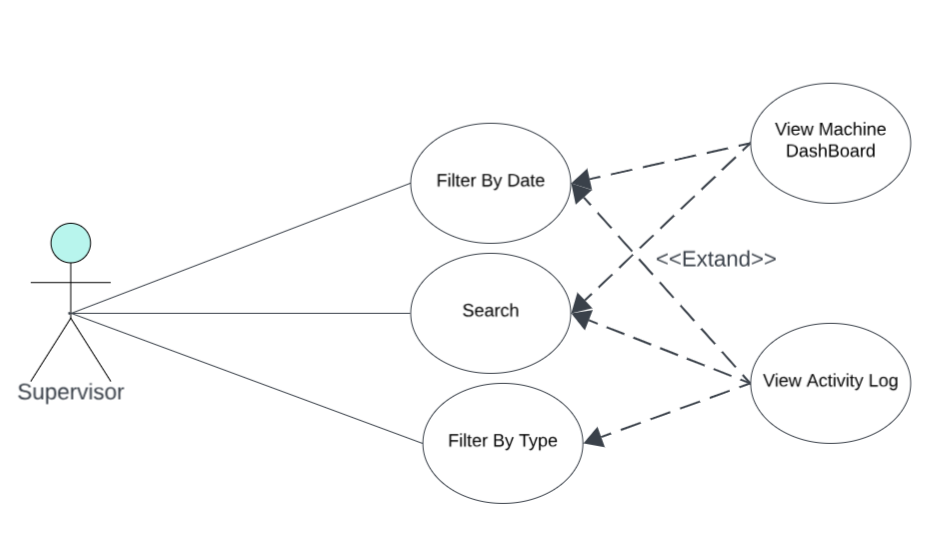
\includegraphics[height=0.5\textheight,keepaspectratio]{./media/MES_Sprint-4-Report/diagrams/useCase/sprint4.png}
      \caption{UML Use Case Diagram --- Administration \& UX.}
      \label{fig:s4-use-case-s4}
\end{figure}

\subsection{Textual Use Case Description}

The following table (Table~\ref{tab:s4-uc-scan-component-s4}) provides the detailed
textual description of the \textit{View Machine Dashboard} use case, which
represents the most significant new administrator workflow in this sprint.

\Needspace{8\baselineskip}
\begin{longtable}{@{} P{0.21\linewidth} P{0.75\linewidth} @{}}
            
      \caption{Textual Use Case Description --- View Machine Dashboard}
      \label{tab:s4-uc-scan-component-s4} \\
      \toprule
      \endfirsthead
      \midrule
      \endhead
      \multicolumn{2}{r}{\small Continued on next page} \\
      \endfoot
      \bottomrule
      \endlastfoot
      
      \textbf{Use Case Name}  & View Machine Dashboard   \\
      \midrule
      \textbf{Primary Actor}  & \userrole{Supervisor} \\
      \midrule
      \textbf{Preconditions}  &                          
      \begin{itemize}[noitemsep, topsep=0pt, partopsep=0pt, leftmargin=*]
      \item The user is authenticated with the \domainterm{Supervisor} role.
      \end{itemize} \\
      \midrule
      \textbf{Postconditions} &                          
      \begin{itemize}[noitemsep, topsep=0pt, partopsep=0pt, leftmargin=*]
      \item A grid of machine cards is displayed, each showing uptime, production
      totals, and scrap for the selected time window.
      \item Changing the time-range selector refreshes all card metrics.
      \end{itemize} \\
      \midrule
      \textbf{Main Scenario}  &                          
      \begin{enumerate}[noitemsep, topsep=0pt, partopsep=0pt, leftmargin=*]
      \item The Supervisor logs in and is routed to \techname{machineList}.
      \item The Supervisor selects \uilabel{Machine Dashboard} in the topBar.
      \item The system POSTs to \apiendpoint{/MESWebService\_fetchMachineDashboard}
      with the default \texttt{hoursBack = 24}.
      \item The backend aggregates execution and progression records and returns
      per-machine metrics.
      \item The Supervisor changes the time range to 48\,h via the AppBar
      dropdown; the page re-fetches and updates.
      \end{enumerate} \\
            
\end{longtable}

\subsection{Sequence Diagrams}

The following sequence diagrams illustrate the communication flow between the
\techname{Flutter} frontend, the \techname{Business Central} OData layer, and
the \techname{AL} business logic for the administrator analytics flows
introduced in Sprint~4.

Figure~\ref{fig:s4-seq-fetch-dashboard} depicts the machine dashboard retrieval
flow. The \techname{AL} layer iterates over all \domainterm{Machine Center}
records and, for each machine, computes the total operation count, cancelled/Interrupted operations,
total production and scrap quantities, and uptime percentage from the corresponding
\techname{Business Central} records before assembling the per-machine KPI rows
returned to the \techname{Flutter} client.

\begin{figure}[H]
      \centering
      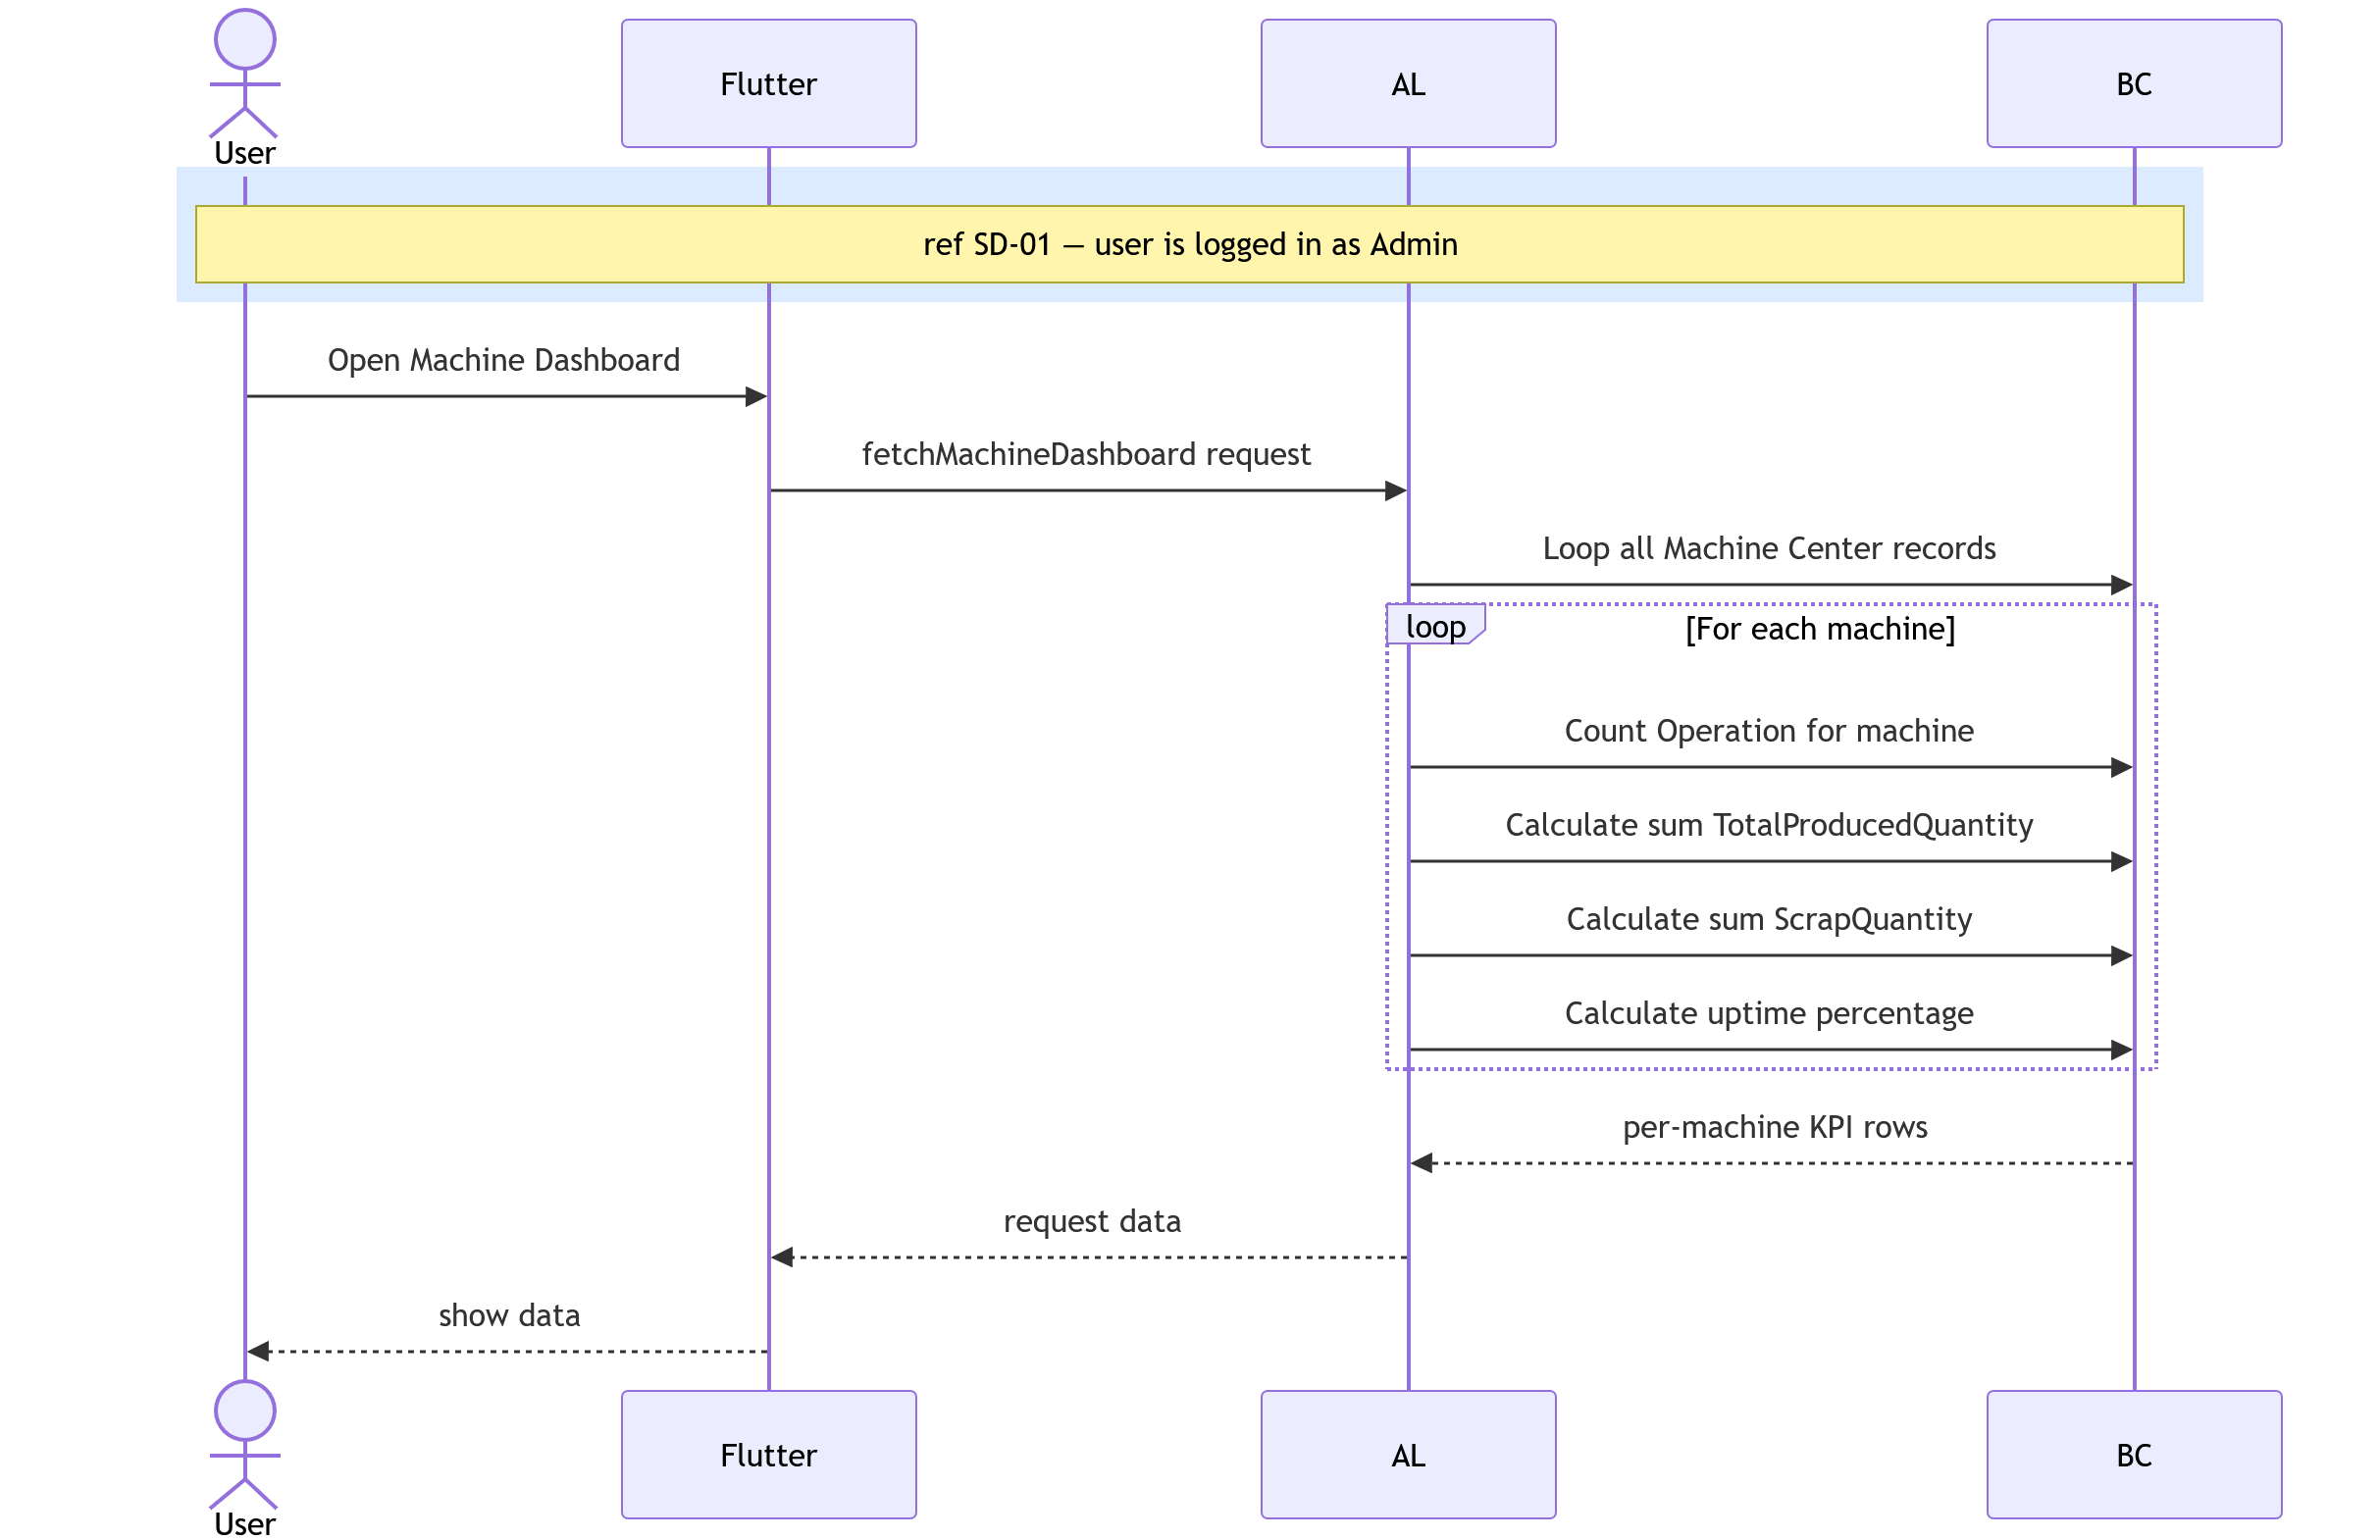
\includegraphics[width=\linewidth,height=0.82\textheight,keepaspectratio]{./media/MES_Sprint-4-Report/diagrams/sequence/machine-dashboard.png}
      \caption{SD-19: Fetch Machine Dashboard.}
      \label{fig:s4-seq-fetch-dashboard}
\end{figure}

%=====SD-19==========================================================
% sequenceDiagram
%       actor User
%       participant Flutter
%       participant Node as Node.js Middleware
%       participant AL
%       participant BC

%       rect rgb(220,235,255)
%           Note over User,BC: ref SD-01 — user is logged in as Admin
%       end

%       User->>Flutter: Open Machine Dashboard
%       Flutter->>Node: POST /api/fetchMachineDashboard 
%       Node->>AL: MESWebService_fetchMachineDashboard 

%       AL->>BC: filter machines to relevant WCs only
%       BC-->>AL: filtered machine list

%       loop For each machine in filtered list
%           AL->>BC: collect the detail from all the necessary records 
%           BC-->>AL: per-machine aggregated KPIs
%       end

%       AL-->>Node: response
%       Node-->>Flutter: response
%       Flutter-->>User: Machine dashboard grid rendered
%====================================================================

Figure~\ref{fig:s4-seq-fetch-activity-log} presents the activity log retrieval
flow. The \techname{AL} layer queries four event tables in parallel;
\domainterm{MES Operation State}, \domainterm{MES Operation Progression},
\domainterm{MES Operation Scrap}, and \domainterm{MES Component Consumption}
, filtering each by the requested time window. For every event row it joins
the associated \domainterm{MES User} and \domainterm{MES Operation Execution}
records to enrich the entry with operator identity and execution context. The
resulting flat event list is returned to the \techname{Flutter} client, which
renders it as a chronological activity table.


\begin{figure}[H]
      \centering
      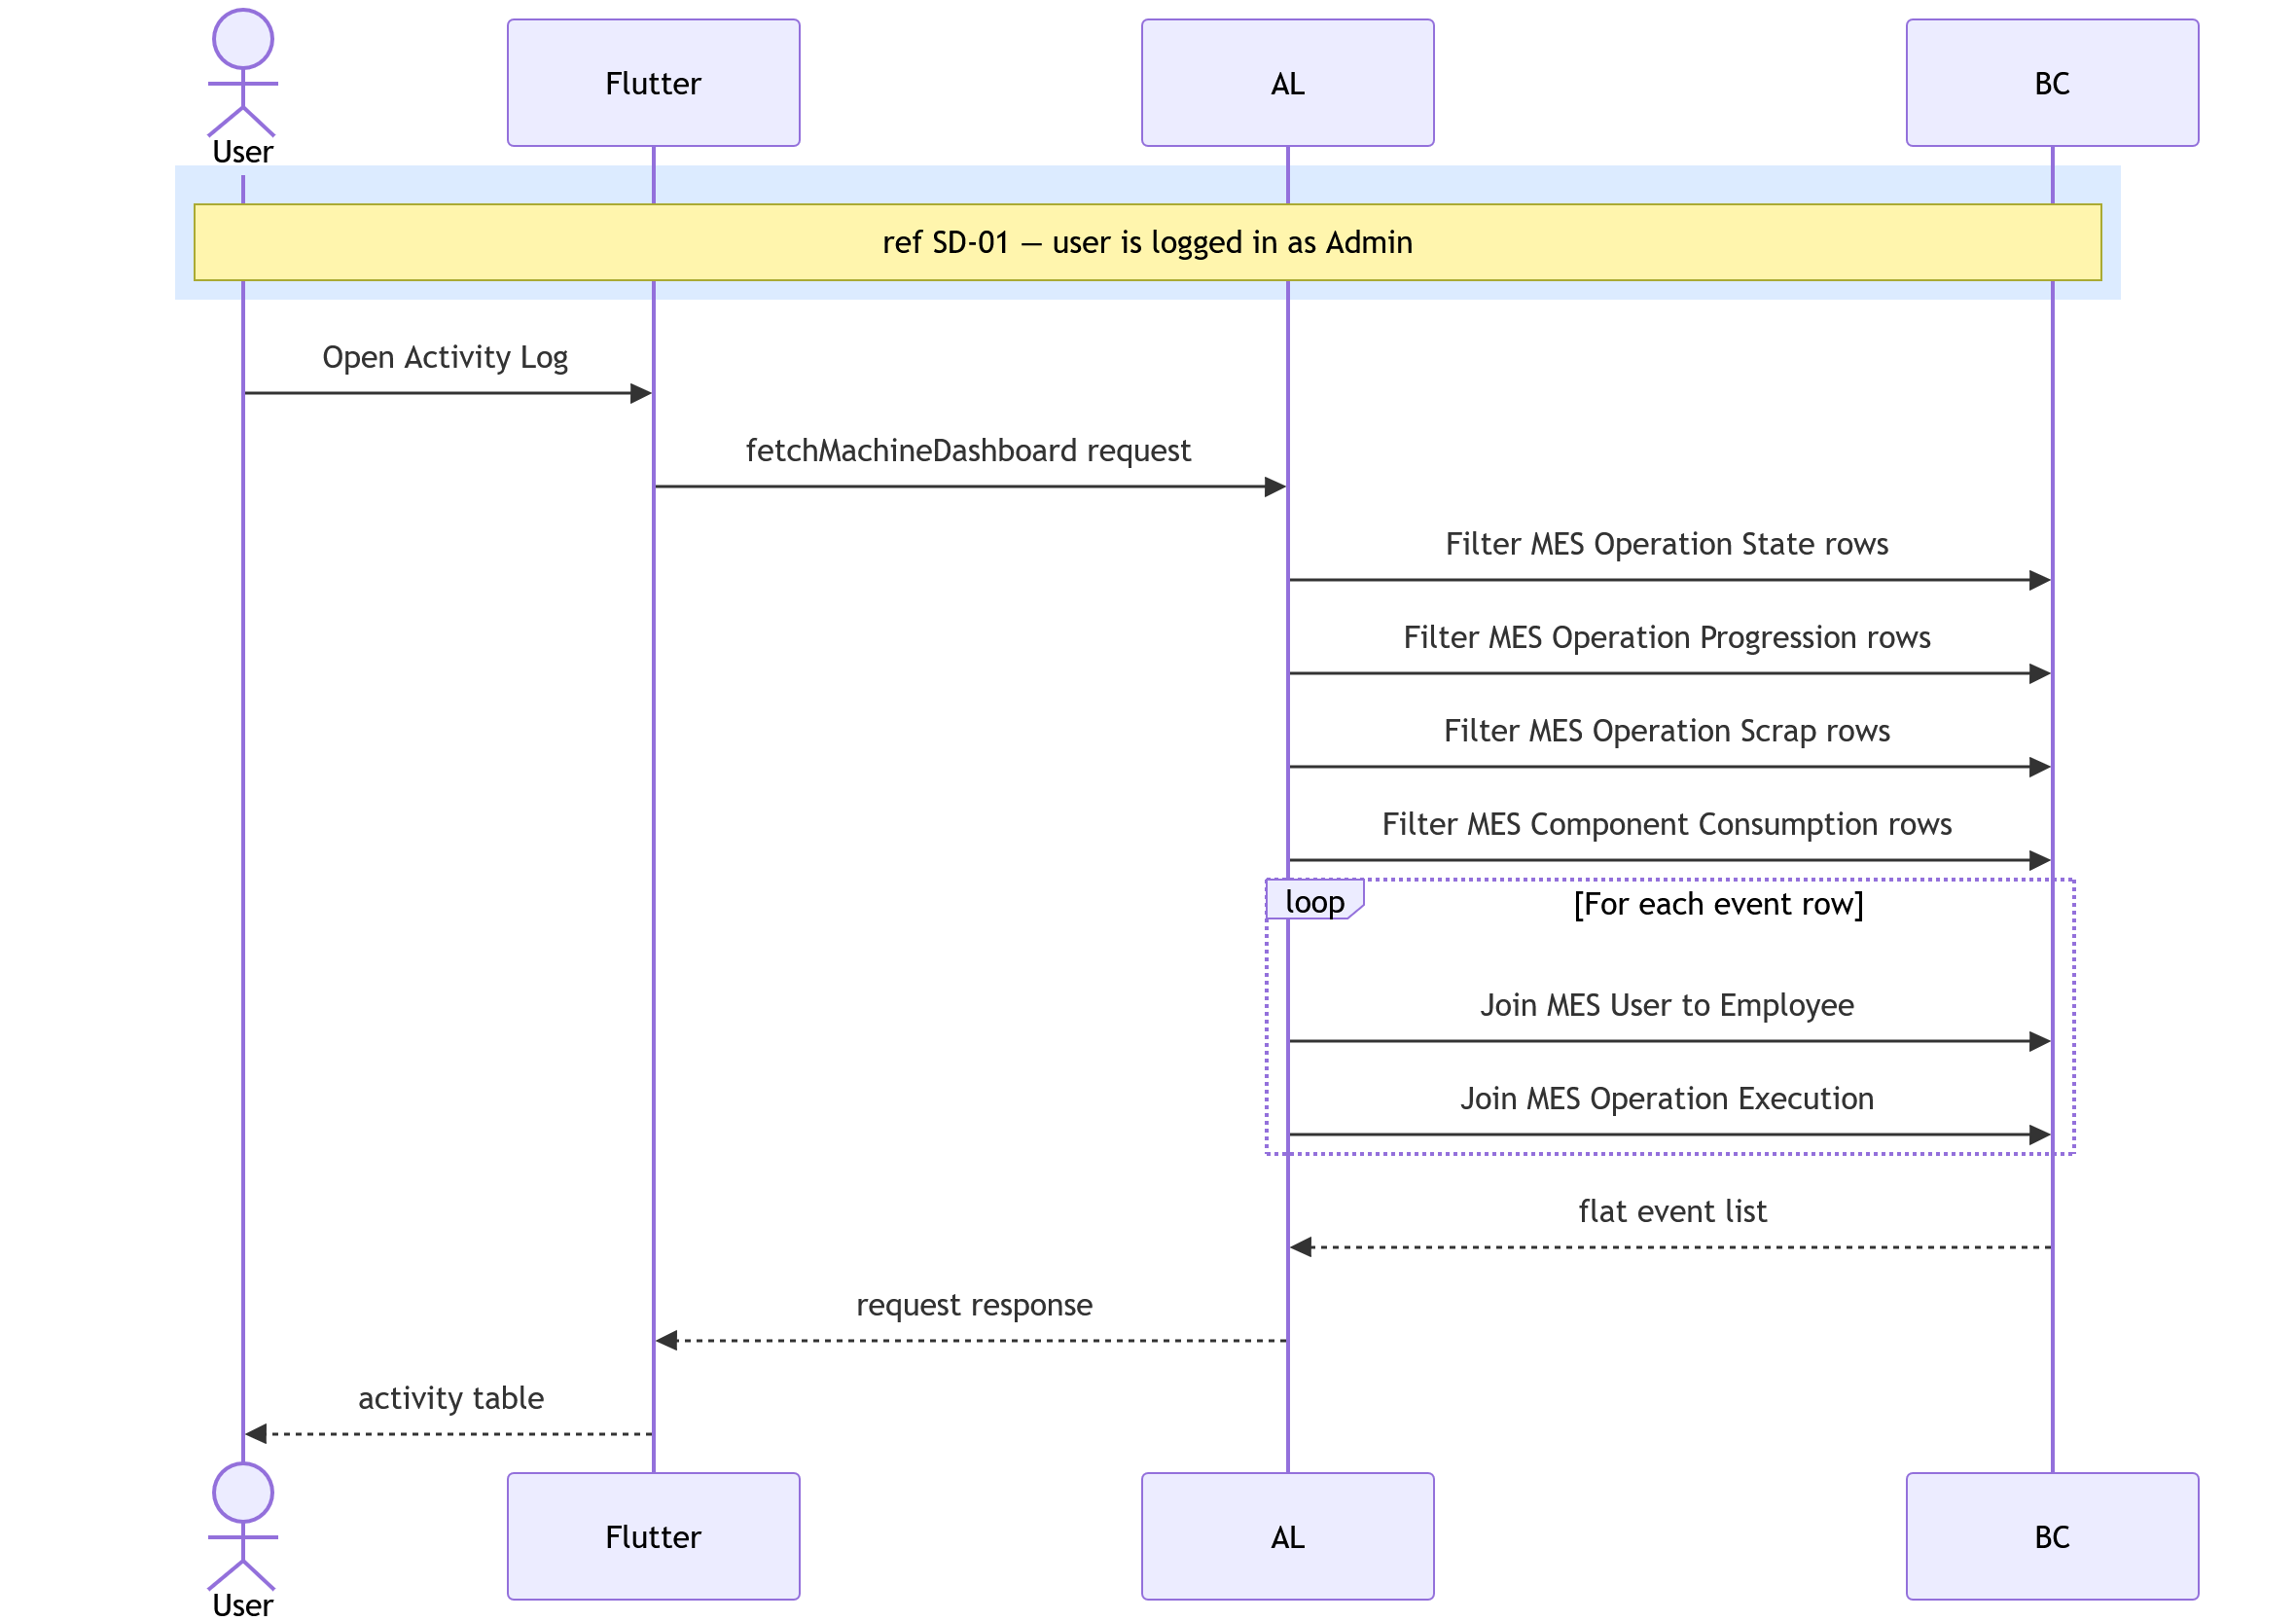
\includegraphics[width=\linewidth,height=0.82\textheight,keepaspectratio]{./media/MES_Sprint-4-Report/diagrams/sequence/activity-log.png}
      \caption{SD-20: Fetch Activity Log.}
      \label{fig:s4-seq-fetch-activity-log}
\end{figure}

%=====SD-20==========================================================
% sequenceDiagram
%       actor User
%       participant Flutter
%       participant Node as Node.js Middleware
%       participant AL
%       participant BC

%       rect rgb(220,235,255)
%           Note over User,BC: ref SD-01 — user is logged in as Admin
%       end

%       User->>Flutter: Open Activity Log 
%       Flutter->>Node: POST /api/fetchActivityLog 
%       Node->>AL: MESWebService_fetchActivityLog 

%       AL->>BC: collect Operation state changes within the cutoff
%       AL->>BC: collect the Operation progress within the cutoff
%       AL->>BC: collect the scrap declarations within the cutoff
%       AL->>BC: collect the component scan within the cutoff

%       AL->>BC: resolve the name of the users


%       AL->>AL: Merge all four event lists into flat chronological array
%       AL-->>Node: response
%       Node-->>Flutter: response
%       Flutter-->>User: Activity log table rendered
%====================================================================

\subsection{Class Diagram}

\begin{figure}[H]
	\centering
	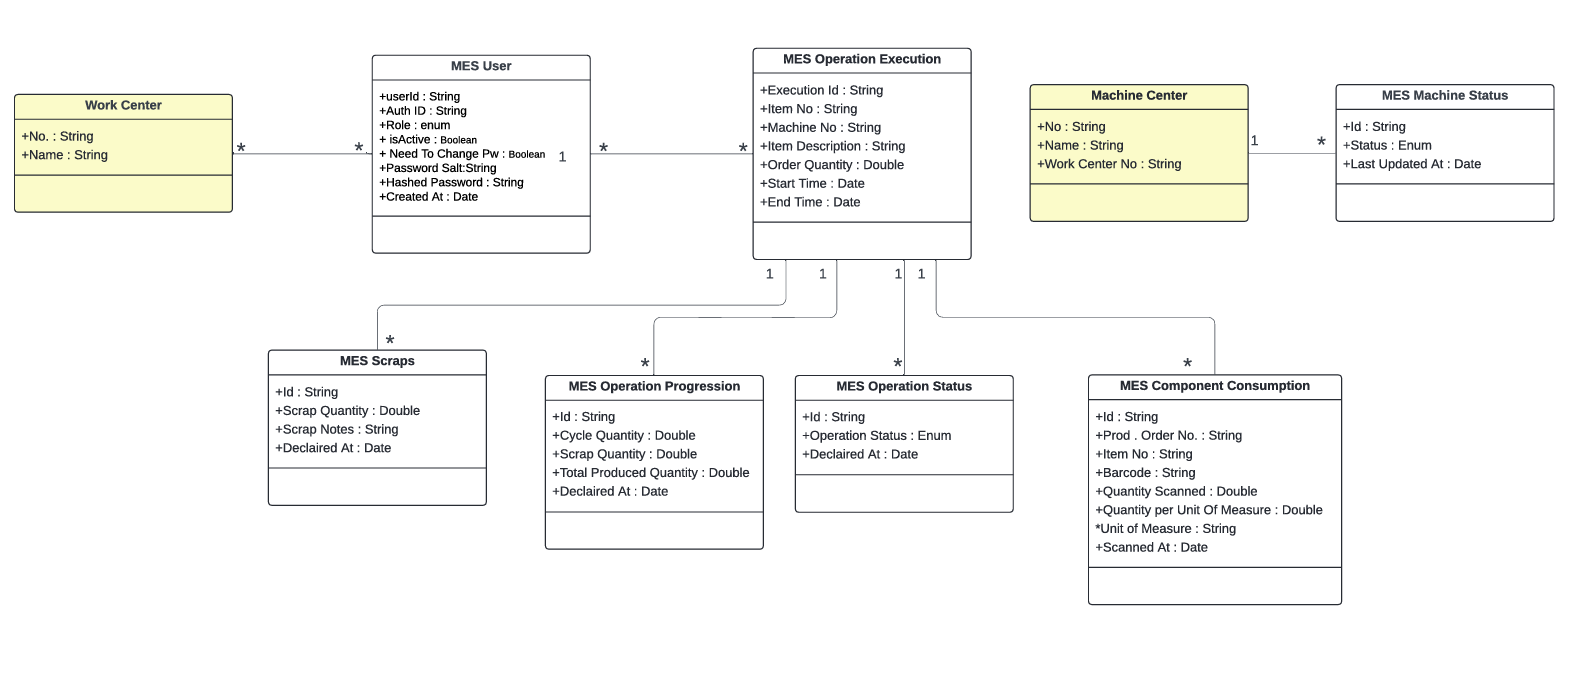
\includegraphics[width=\linewidth,keepaspectratio]{./media/MES_Sprint-4-Report/diagrams/class/sprint4.png}
	\caption{UML Class Diagram.}
	\label{fig:s4-class-diagram}
\end{figure}

% ---------------------------------------------------------------------------
% 4. IMPLEMENTATION
% ---------------------------------------------------------------------------
\section{Implementation}

\subsection{Backend Implementation}

No new \techname{Business Central} tables are introduced in this sprint.
All backend work consists of new query and aggregation procedures added to
\techname{MES Web Service} (codeunit~50126), reading from tables defined in
Sprints~1 through~3.

\subsubsection{Dashboard Aggregation}

\texttt{fetchMachineDashboard()} accepts a \texttt{hoursBack} window and an
optional \texttt{workCenterNoJson} filter. For each \modulename{Machine Center}
it aggregates the matched \modulename{MES Operation Execution} records,
summing \texttt{Cycle Quantity} from linked \modulename{MES Operation
Progression} entries to obtain total produced and scrap counts, and computing
uptime as \texttt{runningMinutes / (hoursBack × 60) × 100}, capped at 100.

\subsubsection{Activity Log Aggregation}

\texttt{fetchActivityLog()} queries four tables within the \texttt{hoursBack}
window --- \modulename{MES Operation State}, \modulename{MES Operation
Progression}, \modulename{MES Operation Scrap}, and \modulename{MES Component
Consumption} --- resolves operator names via the \modulename{Employee} table,
and merges the results into a single descending-timestamp JSON array.

\subsubsection{API Endpoints Added in Sprint 4}

All endpoints are exposed as ODataV4 unbound actions through
\techname{MES Web Service} (codeunit~50126) and are served by the
middleware at:

\begin{center}
  \texttt{middlewareHostURL/api/<endpointName>}
\end{center}

\noindent Each request is forwarded to the \techname{AL} layer as an
ODataV4 action call of the form:

\begin{center}
  \texttt{POST~<baseUrl>/ODataV4/MESWebService\_<ProcedureName>?company=<companyId>}
\end{center}

\begin{longtable}{@{} P{0.48\linewidth} @{\hspace{0.04\linewidth}} P{0.48\linewidth} @{}}
  \caption{New API Endpoints --- Sprint 4}
  \label{tab:s4-api-endpoints}\\
  \toprule
  \textbf{Endpoint} & \textbf{Endpoint}\\
  \midrule
  \endfirsthead
  \toprule
  \textbf{Endpoint} & \textbf{Endpoint}\\
  \midrule
  \endhead
  \multicolumn{2}{r}{\small Continued on next page}\\
  \endfoot
  \bottomrule
  \endlastfoot

  \apiendpoint{fetchMachineDashboard} & \apiendpoint{fetchActivityLog} \\ 
\end{longtable}

\subsection{Frontend Implementation}

\subsubsection{Shared HTTP Infrastructure}

All sprint services (including retroactively migrated ones) share a
\techname{HttpClient} and \techname{HttpResponseParser} layer, replacing
the inline \texttt{http.post} calls from Sprint~1.
\techname{HttpClient.post()} is a centralised wrapper that injects
JSON headers and encodes the request body.
\techname{HttpResponseParser} exposes four static helpers:
\texttt{parseList()} and \texttt{parseObject()} decode OData list and
single-object responses respectively; \texttt{parseWriteResult()} decodes
write responses and surfaces backend errors; \texttt{\_assertSuccess()}
validates HTTP status codes and throws a structured exception on non-2xx
responses.

\subsubsection{Provider Architecture}

\begin{longtable}{@{} P{0.30\linewidth} P{0.65\linewidth} @{}}
  \caption{Provider Responsibilities --- Sprint 4 Additions}
  \label{tab:s4-providers-s4} \\
  \toprule
  \textbf{Provider}             & \textbf{Responsibility} \\
  \midrule
  \endfirsthead
  \toprule
  \textbf{Provider}             & \textbf{Responsibility} \\
  \midrule
  \endhead
  \multicolumn{2}{r}{\small Continued on next page} \\
  \endfoot
  \bottomrule
  \endlastfoot

  \techname{LogProvider}        &
   Owns dashboard and activity log fetch calls; exposes \texttt{selectedHours},
   \texttt{hourOptions}, and \texttt{setHours()} shared between the two admin pages. \\
  \addlinespace
  \techname{MesBarcodeProvider} & 
  Exposes \texttt{fetchAllBarcodes()}; resolves the session token automatically from
  \techname{AuthProvider}. \\
\end{longtable}

\subsubsection{User Interface}


\begin{figure}[H]
  \centering
  \setlength{\fboxsep}{5pt}
  \colorbox{black}{%
    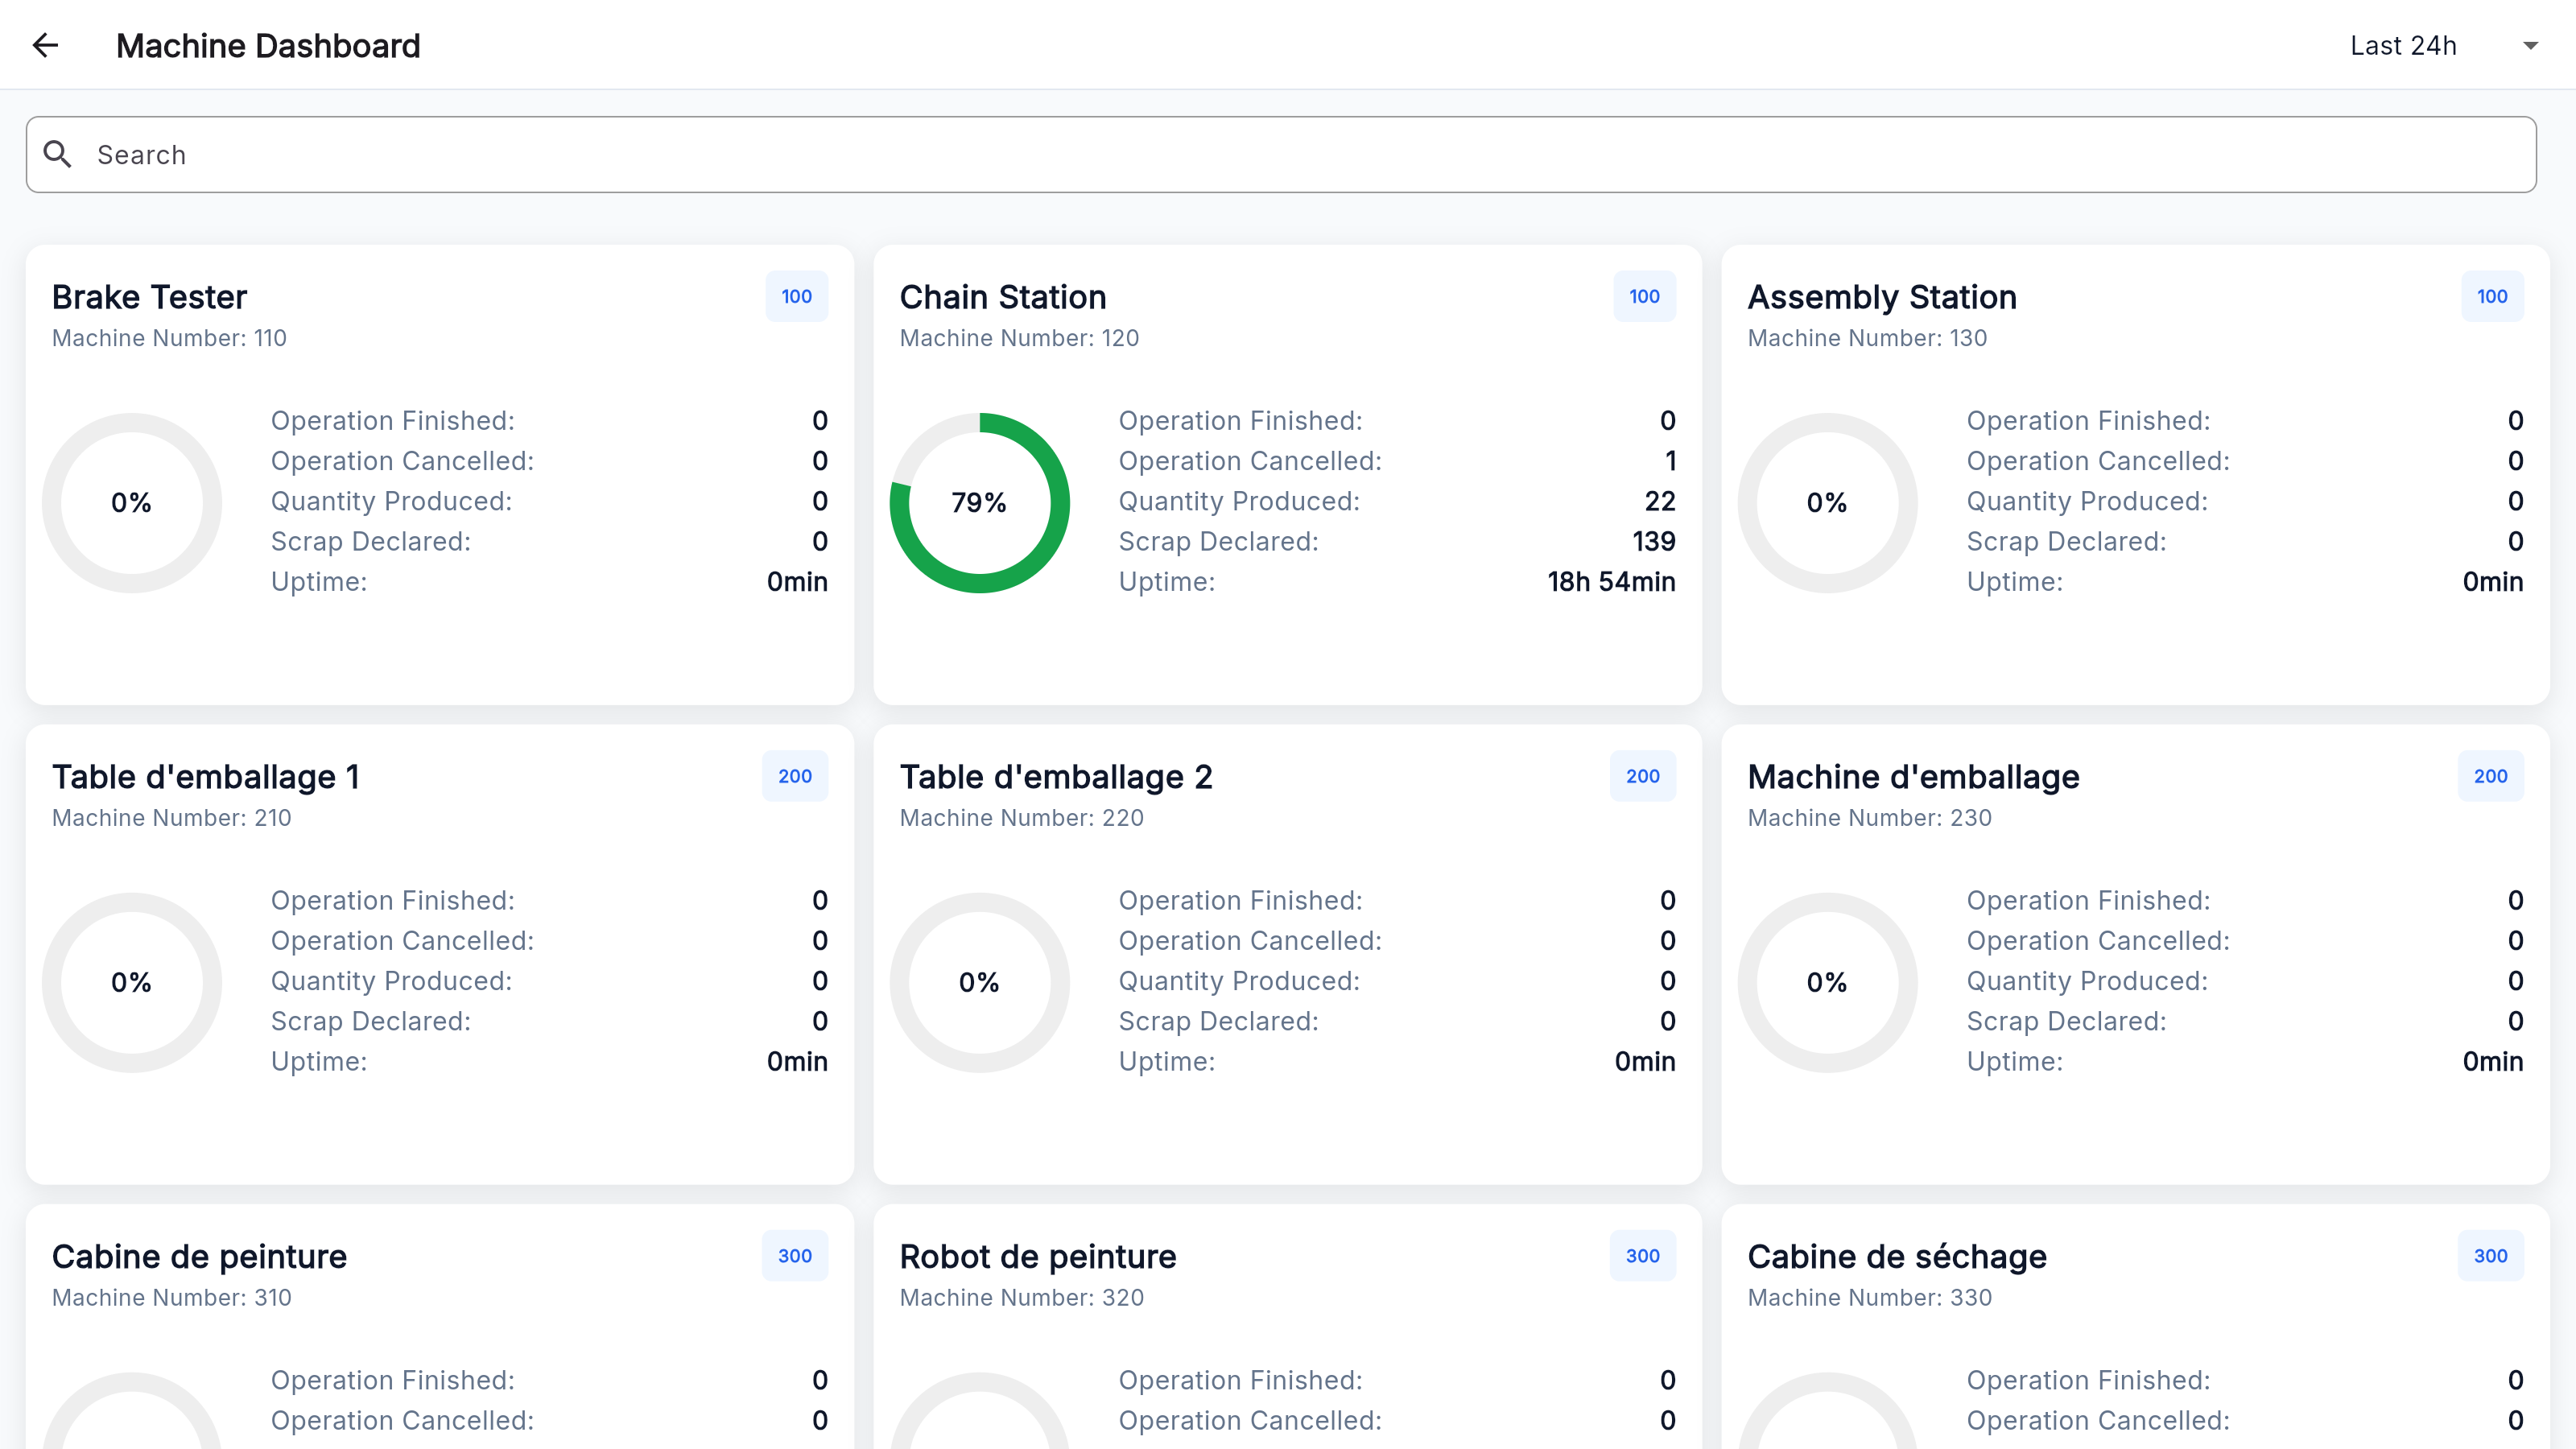
\includegraphics[height=0.3\textheight,keepaspectratio]{./media/MES_Sprint-4-Report/UI/dashboard/wide.png}%
    \hspace{\fboxsep}%
    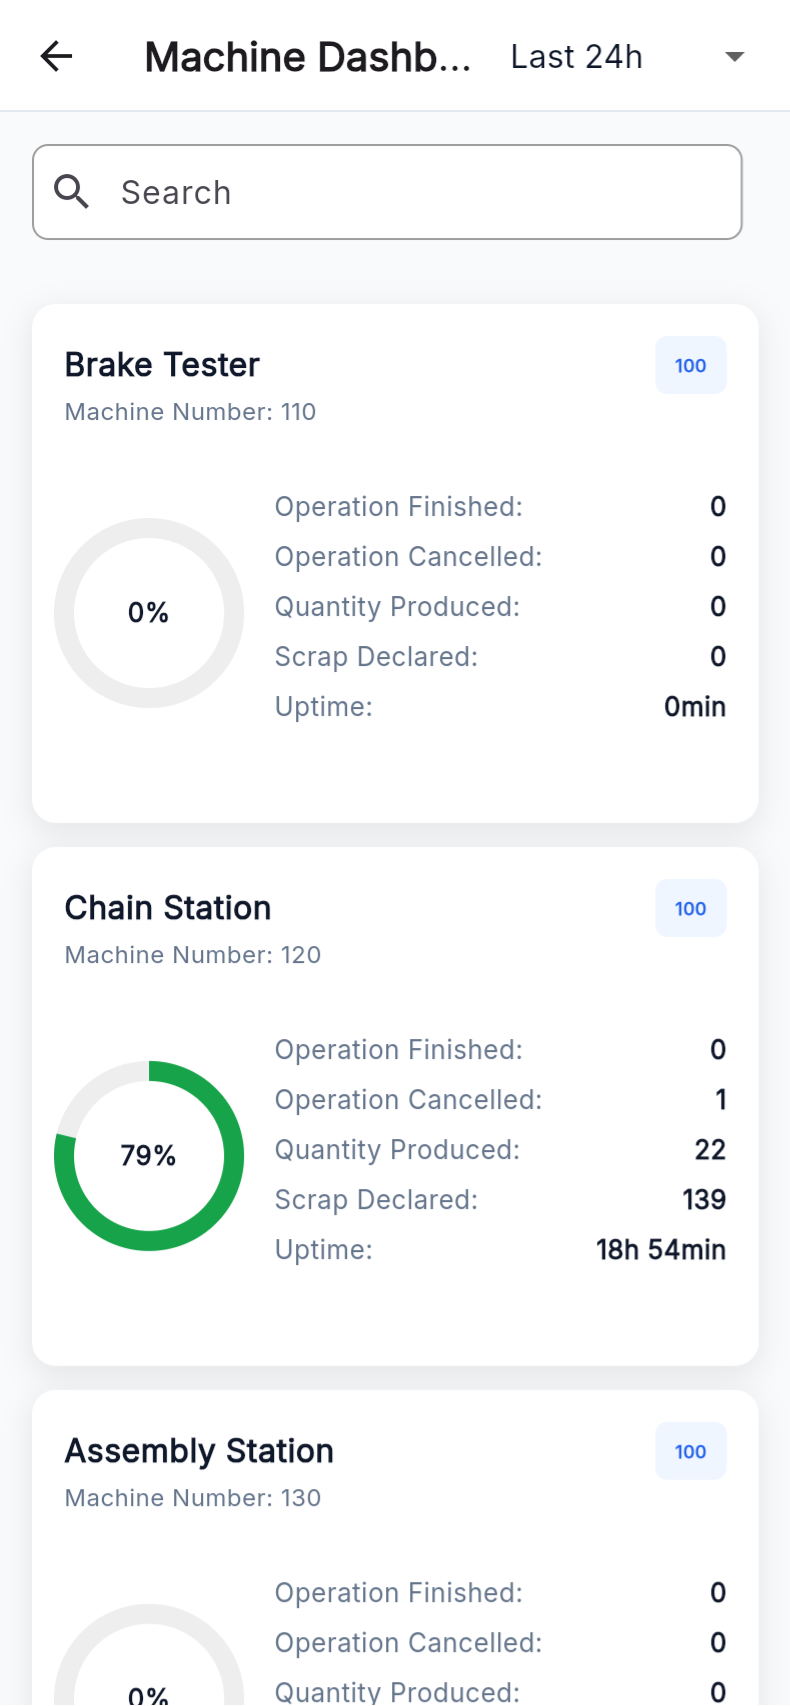
\includegraphics[height=0.3\textheight,keepaspectratio]{./media/MES_Sprint-4-Report/UI/dashboard/small.png}%
  }
  \caption{\uilabel{Machine Dashboard Page} --- desktop and mobile views.}
  \label{fig:s4-ui-machine-dashboard}
\end{figure}

Figures~\ref{fig:s4-ui-machine-dashboard} and~\ref{fig:s4-ui-activity-log} illustrate
the two pages. The \uilabel{Machine Dashboard Page} renders one card per machine
with a circular uptime indicator and four metric rows (finished operations, 
Cancelled and Interrupted operations, produced, scrap, uptime), and
an AppBar time-range dropdown that re-fetches on change. The \uilabel{Activity Log Page}
presents a paginated, newest-first event list where each row shows a type icon, 
operator, machine, and expandable action text; AppBar dropdowns filter by type and 
time range.

\begin{figure}[H]
  \centering
  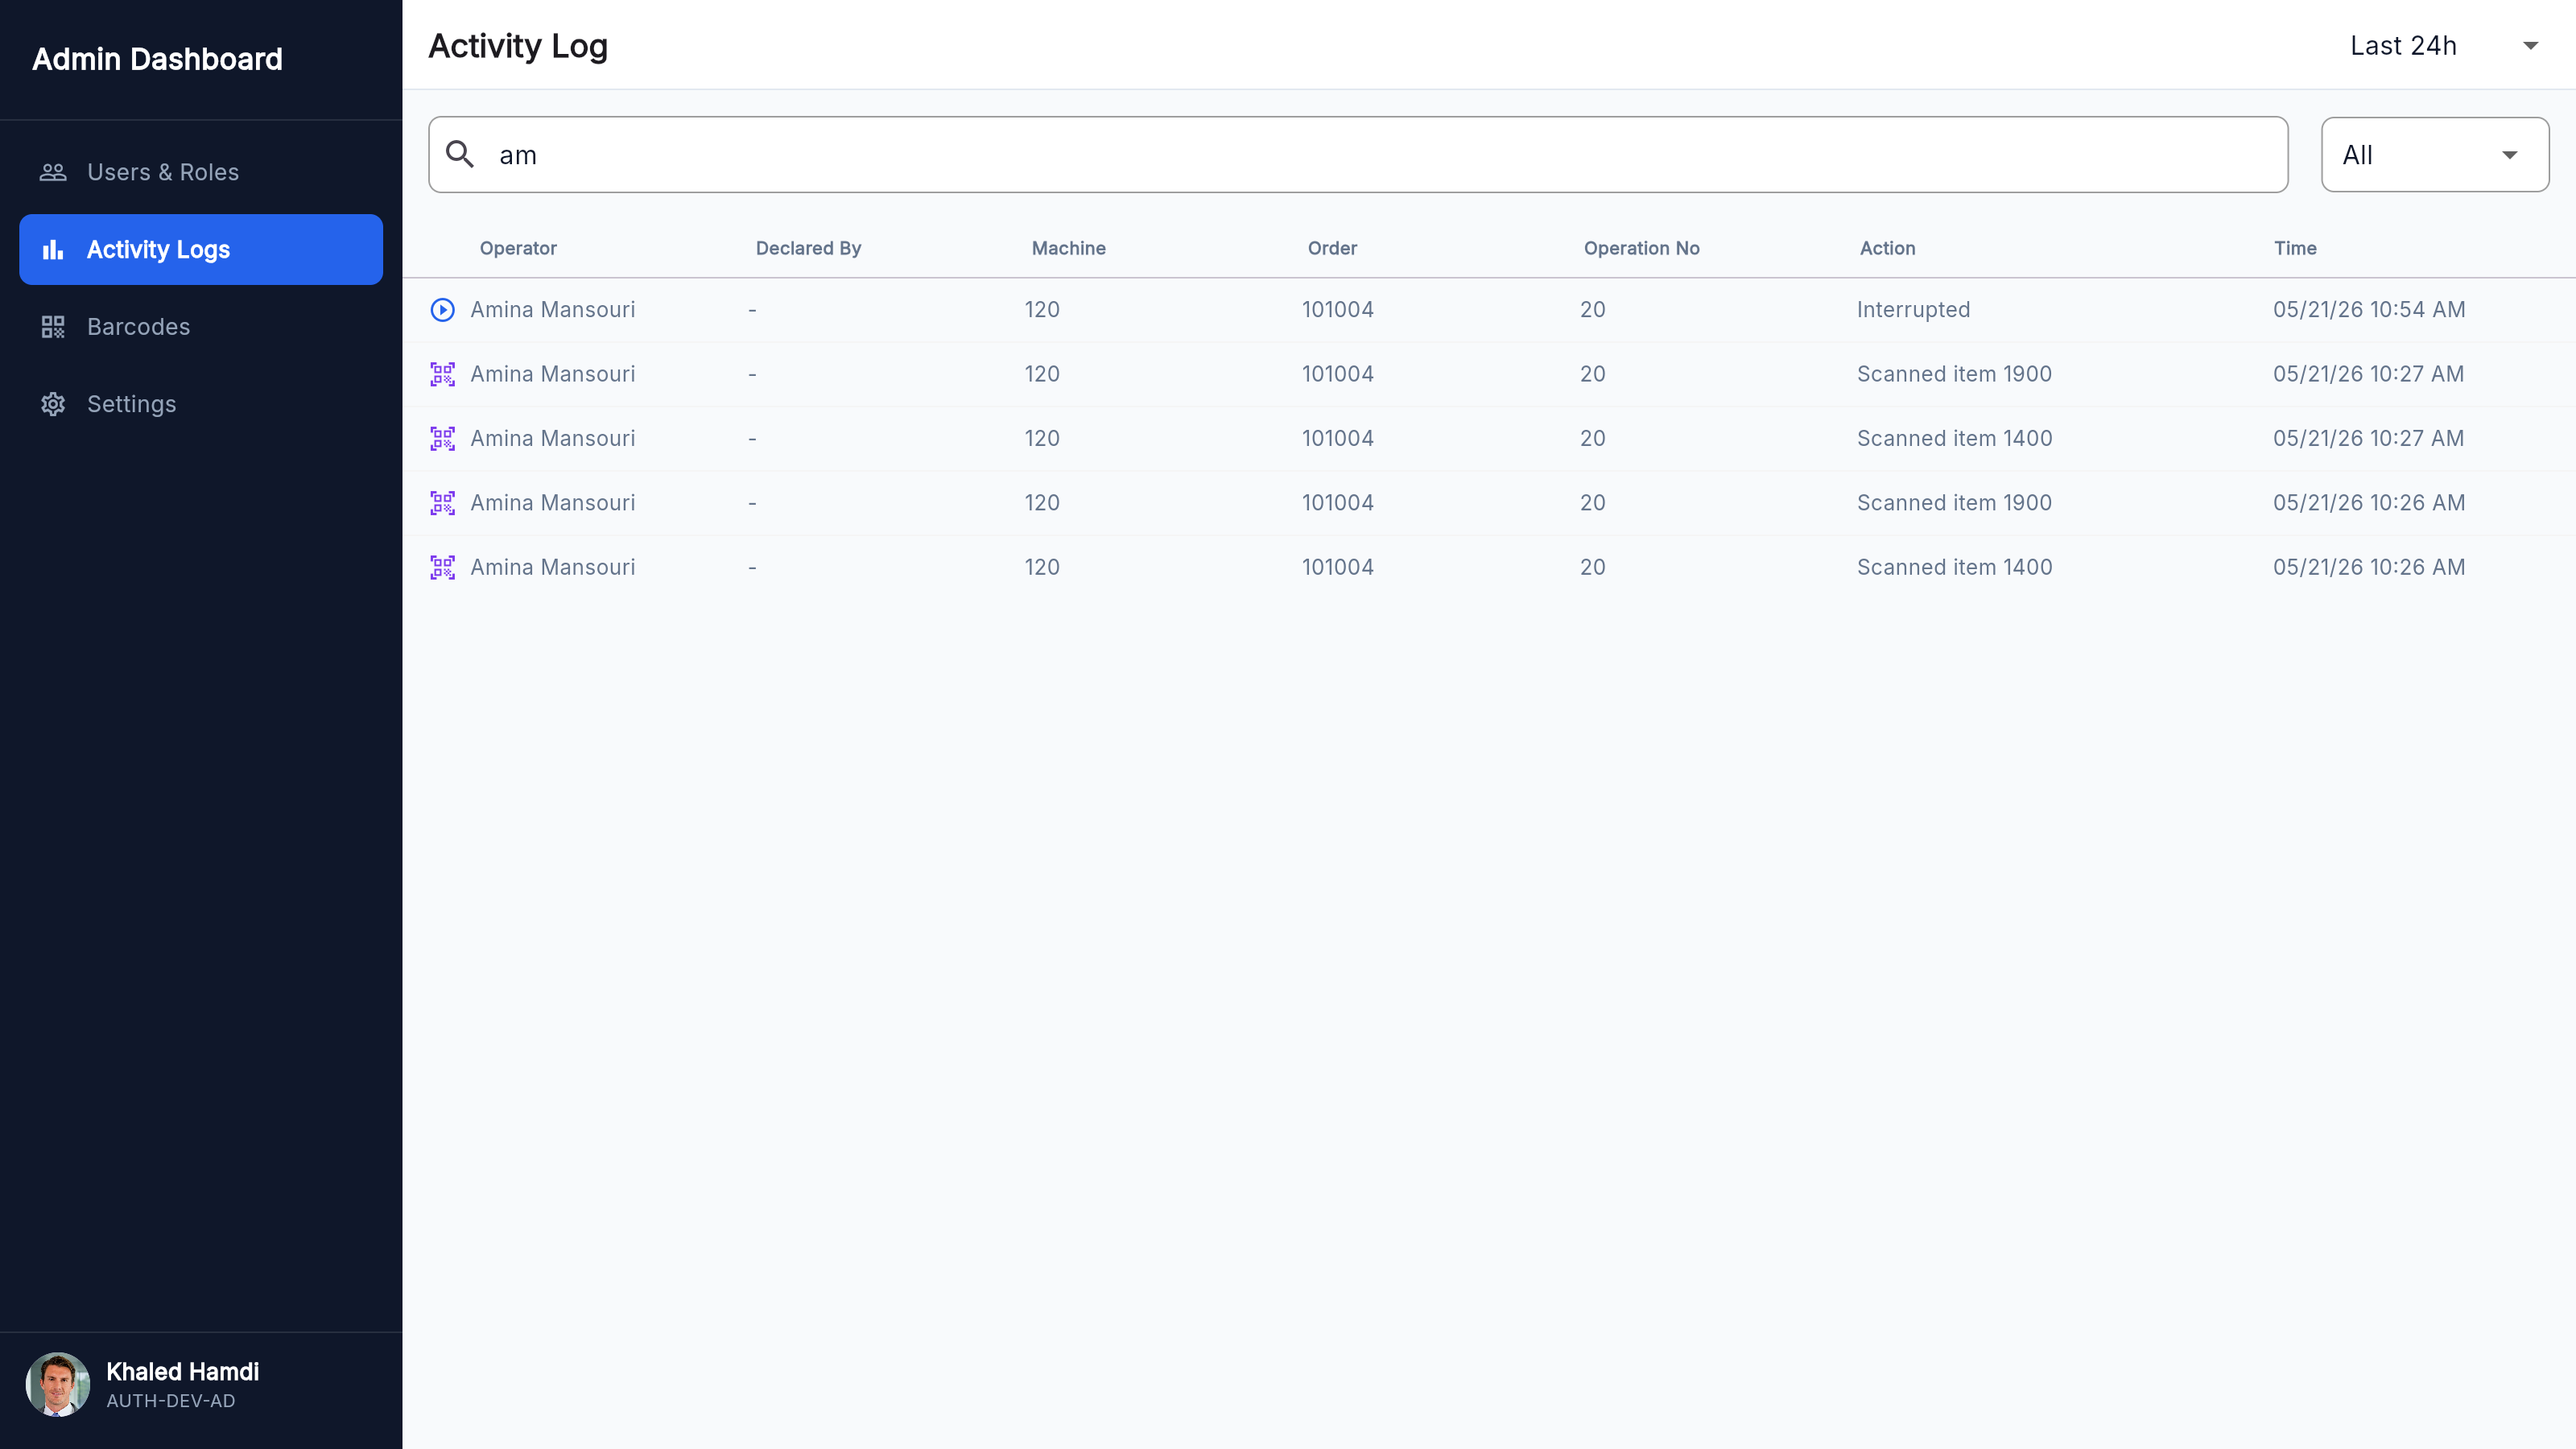
\includegraphics[height=0.3\textheight,keepaspectratio]{./media/MES_Sprint-4-Report/UI/activityLog/wide.png}
  \caption{\uilabel{Activity Log Page} --- desktop and mobile views.}
  \label{fig:s4-ui-activity-log}
\end{figure}
\section{Test and validation}
\subsection{Integration test}

For integration testing, we chose Postman, a powerful and user-friendly tool for API evaluation. Figure~\ref{fig:s4-test-postman-activityLog} shows a test case for the \apiendpoint{/activityLog} endpoint.

\begin{figure}[H]
  \centering
  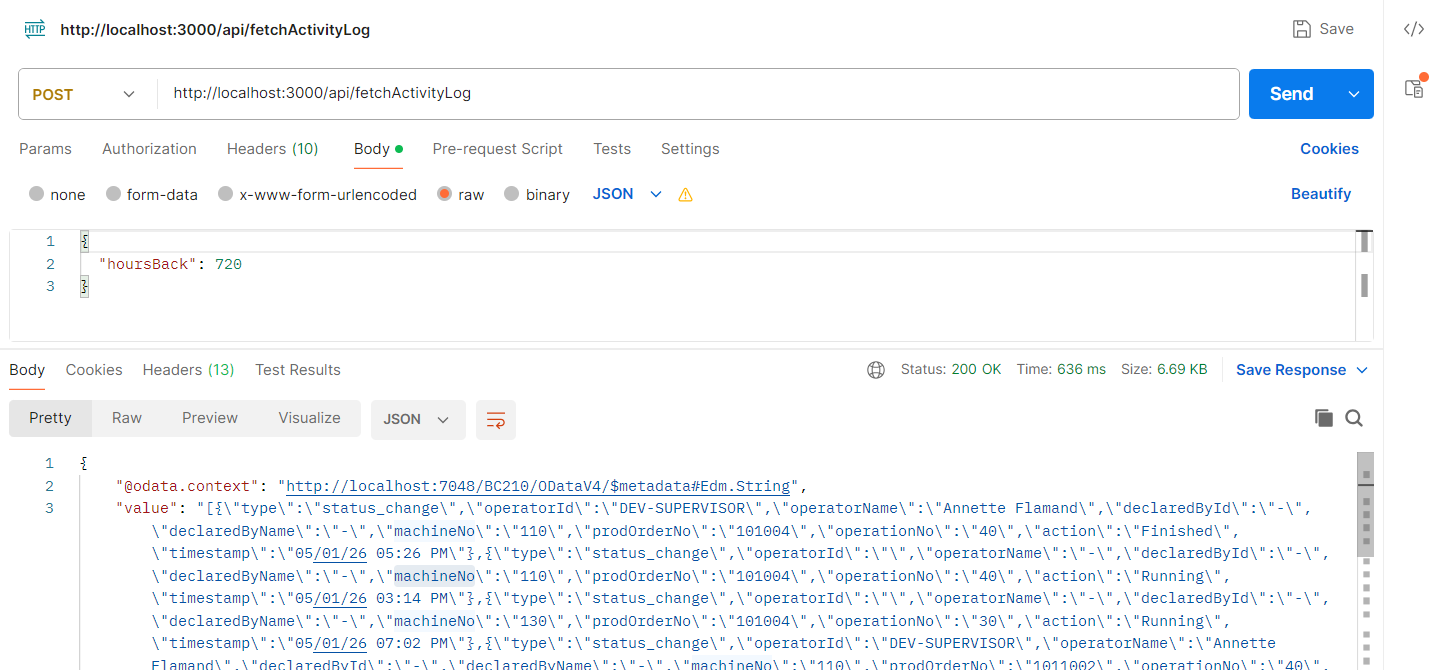
\includegraphics[width=\linewidth,keepaspectratio]{./media/MES_Sprint-4-Report/test/postman/fetchActivityLog.png}
  \caption{Postman endpoint test --- fetchActivityLog.}
  \label{fig:s4-test-postman-activityLog}
\end{figure}

Figure~\ref{fig:s4-test-postman-machineDashboard} shows a test case for the \apiendpoint{/MachineDashboard} endpoint.

\begin{figure}[H]
  \centering
  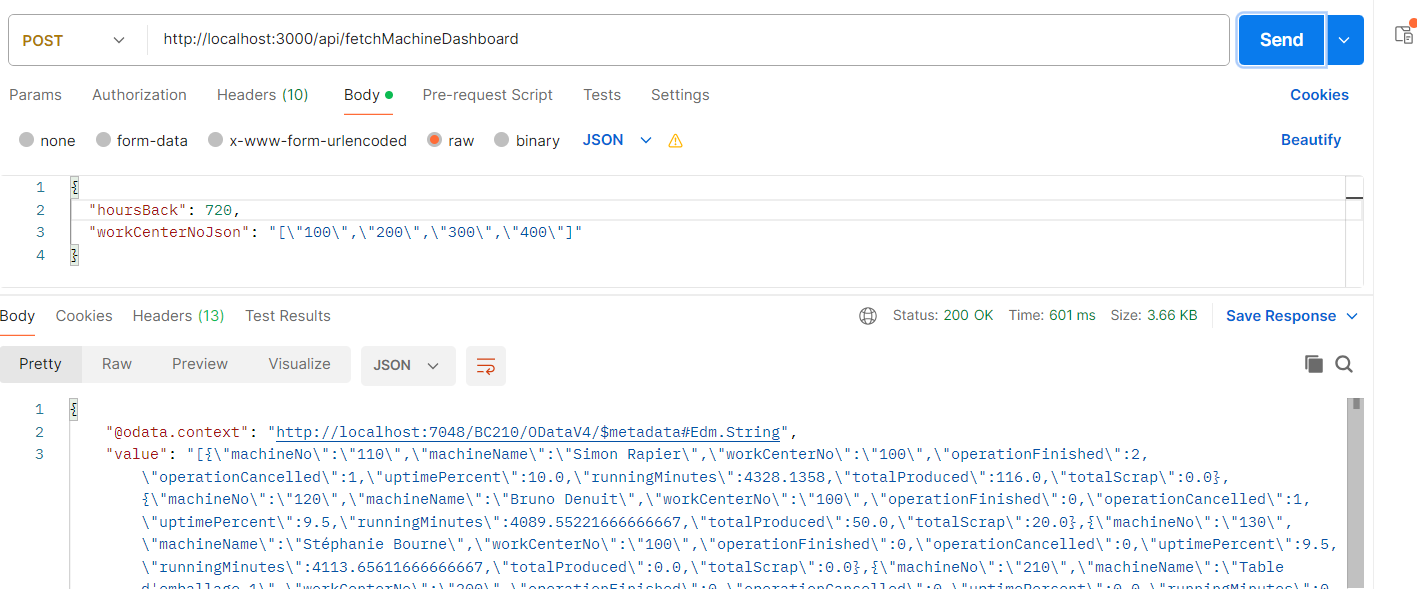
\includegraphics[width=\linewidth,keepaspectratio]{./media/MES_Sprint-4-Report/test/postman/fetchMachineDashboard.png}
  \caption{Postman endpoint test --- fetchMachineDashboard.}
  \label{fig:s4-test-postman-machineDashboard}
\end{figure}

% ---------------------------------------------------------------------------
% CONCLUSION
% ---------------------------------------------------------------------------
\phantomsection
\section*{Conclusion}
\addcontentsline{toc}{section}{Conclusion}

This sprint completed the \domainterm{MES} solution by delivering the
administration layer and cross-cutting quality-of-life features. Administrators
can now monitor the production health of the entire facility through a
configurable machine performance dashboard, audit all operator and machine
actions through a paginated activity log, and manage users from a persistent
navigation shell without losing context between sections. All users benefit from
full internationalisation covering English, French, and Arabic with automatic
right-to-left layout, and from guided coach-mark tutorials that ease onboarding
for first-time users.


% ---------------------------------------------------------------------------
% Sprint 5 AI Assistant \& Analytical Intelligence.
% ---------------------------------------------------------------------------
\chapter{Sprint 5 AI Assistant \& Analytical Intelligence.}
\graphicspath{{./media/MES_Sprint-5-Report/}}
\minitoc
\newpage
\section*{Introduction}
\addcontentsline{toc}{section}{Introduction}

This sprint report covers \textbf{Domain 5: AI Assistant \& Analytical Intelligence}. Building upon the complete shop-floor execution loop established in the previous sprints, this sprint delivers the AI layer of the MES system: a natural-language chat assistant embedded in the Flutter frontend, a \techname{Node.js} reverse proxy middleware that bridges the Flutter app to both \techname{Business Central} and a locally-hosted Python AI agent, and the Python agent itself. The agent provides deterministic tool orchestration, multi-provider LLM synthesis, fuzzy machine name resolution, multi-machine fan-out, production data enrichment, and contextual redirect actions. The result is a conversational interface that operators and supervisors can use to query real-time machine status, production orders, scrap rates, BOM consumption, delays, and operator performance without leaving the MES application.

% ---------------------------------------------------------------------------
% 1. SPRINT BACKLOG
% ---------------------------------------------------------------------------
\section{Sprint Backlog}

This sprint covers \textbf{Domain 5:} \textbf{\domainterm{AI Assistant \& Analytical Intelligence}}.

\begin{longtable}{@{} P{0.09\linewidth} P{0.38\linewidth} P{0.49\linewidth} @{}}
	\caption{US-5.1 --- AI Chat Interface}
	\label{tab:s5-US-5.1} \\
	\toprule
	\textbf{ID} & \textbf{User Story} & \textbf{Acceptance Criteria} \\
	\midrule
	\endfirsthead
	\toprule
	\textbf{ID} & \textbf{User Story} & \textbf{Acceptance Criteria} \\
	\midrule
	\endhead
	\multicolumn{3}{r}{\small Continued on next page} \\
	\endfoot
	\bottomrule
	\endlastfoot

	\textbf{US-5.1}
	& As an \userrole{Operator} or \userrole{Supervisor}, I need an embedded chat assistant in the MES app so that I can query production data using natural language without switching tools.
	& \noindent\textit{Flutter:}
	\begin{itemize}[noitemsep, topsep=0pt, partopsep=0pt, leftmargin=*]
		\item Create model \techname{ConversationTurn}, \techname{AiRedirectAction}, and \techname{AiChatResponse}.
		\item Create \techname{AiChatService} to POST to the \texttt{/api/ai/chat} endpoint.
		\item Create \techname{AiChatProvider} to manage conversation history, loading state, and the last response.
		\item Create page \techname{AiChatPage} supporting both modal dialog and embedded side-panel modes.
		\item Integrate the chat panel into \techname{MachineListPage} as a collapsible side panel on desktop and a modal dialog on mobile.
		\item Implement \techname{\_handleAction()} to process \techname{AiRedirectAction} objects (redirect to machine, operation, or machine list).
	\end{itemize} \\
	\midrule

	\textbf{US-5.2}
	& As a \userrole{Supervisor}, I need the AI to understand questions about multiple machines simultaneously so that I can get fleet-wide answers from a single query.
	& \noindent\textit{Python AI Agent:}
	\begin{itemize}[noitemsep, topsep=0pt, partopsep=0pt, leftmargin=*]
		\item Implement composite query detection in \modulename{composite.py}.
		\item Implement fan-out batch execution across machines using \texttt{asyncio.gather} in batches of 4.
		\item Implement \texttt{build\_composite\_context()} to produce a compact markdown context for the LLM.
		\item Cap fan-out at 12 machines to prevent timeout.
		\item Integrate the composite path into \techname{MESAgentOrchestrator}.
	\end{itemize} \\
	\midrule

	\textbf{US-5.3}
	& As an \userrole{Operator} or \userrole{Supervisor}, I need to refer to machines by colloquial names or partial identifiers so that I do not need to memorise exact machine codes.
	& \noindent\textit{Python AI Agent:}
	\begin{itemize}[noitemsep, topsep=0pt, partopsep=0pt, leftmargin=*]
		\item Implement \texttt{build\_machine\_index()} to build a lookup structure from the machine list.
		\item Implement a five-tier fuzzy resolution cascade in \texttt{resolve\_machine()} (exact canonical, normalised exact, digit suffix, ID prefix/suffix, token overlap, edit distance).
		\item Define \texttt{MIN\_CONFIDENCE = 0.45} and \texttt{HIGH\_CONFIDENCE = 0.85} thresholds.
		\item Implement \texttt{format\_candidates\_for\_llm()} to surface ambiguous matches to the user.
		\item Integrate resolver into orchestrator when \texttt{unresolved\_machine\_ref} is set.
	\end{itemize} \\
	\midrule

	\textbf{US-5.4}
	& As a \userrole{Supervisor}, I need the AI to alert me to overdue orders, excessive pauses, and high scrap rates so that I can take corrective action without manually reviewing dashboards.
	& \noindent\textit{Python AI Agent:}
	\begin{itemize}[noitemsep, topsep=0pt, partopsep=0pt, leftmargin=*]
		\item Implement \texttt{enrich\_deadlines()} in \modulename{data\_analysis.py} to compute \texttt{hours\_until\_deadline}, \texttt{is\_overdue}, and \texttt{risk\_level} per order.
		\item Implement \texttt{analyse\_scrap()} to compute \texttt{scrap\_rate}, \texttt{severity} (ok / warning / critical), \texttt{spike\_detected}, and \texttt{interpretation}.
		\item Implement \texttt{analyse\_velocity()} to compute \texttt{units\_per\_hour}, \texttt{required\_rate}, \texttt{projected\_end}, and \texttt{velocity\_status}.
		\item Wire enrichment results into the LLM context block before synthesis.
	\end{itemize} \\
	\midrule

	\textbf{US-5.5}
	& As an \userrole{Operator} or \userrole{Supervisor}, I need intent classification to work reliably without requiring a network call to an LLM so that the assistant remains responsive even when the LLM is slow.
	& \noindent\textit{Python AI Agent:}
	\begin{itemize}[noitemsep, topsep=0pt, partopsep=0pt, leftmargin=*]
		\item Implement \modulename{intent.py} with 12 intent classes and a priority-ordered regex rule cascade.
		\item Implement extraction helpers: \texttt{\_extract\_machine\_no()}, \texttt{\_extract\_machine\_ref()}, \texttt{\_extract\_order\_no()}, \texttt{\_extract\_op\_no()}, \texttt{\_extract\_hours()}.
		\item Define the \techname{ToolStep} and \techname{ToolChain} data types.
		\item Implement \modulename{llm\_intent.py} as the primary LLM-based classifier with automatic fallback to regex.
	\end{itemize} \\
	\midrule

	\textbf{US-5.6}
	& As a \userrole{Supervisor}, I need the AI to provide clickable navigation actions in its replies so that I can jump directly to a relevant machine or operation.
	& \noindent\textit{Python AI Agent:}
	\begin{itemize}[noitemsep, topsep=0pt, partopsep=0pt, leftmargin=*]
		\item Define the \techname{ActionType} enum with 5 redirect types in \modulename{models.py}.
		\item Implement \texttt{\_parse\_actions()} in the orchestrator to extract a \texttt{```actions```} JSON block from the LLM reply.
		\item Return up to 4 \techname{RedirectAction} objects in \techname{ChatResponse}.
	\end{itemize}
	\noindent\textit{Flutter:}
	\begin{itemize}[noitemsep, topsep=0pt, partopsep=0pt, leftmargin=*]
		\item Render \techname{\_ActionButtons} in \techname{AiChatPage} as a \texttt{Wrap} of tappable \texttt{ElevatedButton}s below each assistant reply.
		\item Implement \texttt{\_handleAction()} routing per action type.
	\end{itemize} \\

\end{longtable}

% ---------------------------------------------------------------------------
% 2. BUSINESS RULES
% ---------------------------------------------------------------------------
\section{Business Rules}

\Needspace{10\baselineskip}
\begin{longtable}{@{} P{0.30\linewidth} P{0.65\linewidth} @{}}
	\caption{Business Rules}
	\label{tab:s5-Business-Rules}\\
	\toprule
	\textbf{ID: Business Rule} & \textbf{Description} \\
	\midrule
	\endfirsthead
	\toprule
	\textbf{ID: Business Rule} & \textbf{Description} \\
	\midrule
	\endhead
	\multicolumn{2}{r}{\small Continued on next page} \\
	\endfoot
	\bottomrule
	\endlastfoot

	\multicolumn{2}{@{}l}{\textbf{AI Intent Classification Rules}} \\
	\midrule

	\businessrule{BR-AI-001}: Two-Tier Classification with Mandatory Fallback &
	The primary classifier (\modulename{llm\_intent.py}) sends a structured prompt to the LLM and validates the returned JSON plan against a schema. If the LLM response is malformed, missing required fields, references an unknown tool name, or contains duplicate \texttt{result\_key} values, the system falls back unconditionally to the deterministic regex classifier (\modulename{intent.py}). The fallback reason is recorded in the \domainterm{ThinkingBlock} but never surfaced to the end user. \\
	\midrule

	\businessrule{BR-AI-002}: LLM Does Not Control Tool Selection &
	The LLM's role is limited to producing a \emph{plan} (a list of tool names and arguments). Actual tool execution, access-control checks, slot resolution, and enrichment are performed entirely in Python. No tool is ever called solely on the LLM's instruction without passing through Python validation. This prevents prompt-injection attacks from influencing which data is fetched. \\
	\midrule

	\businessrule{BR-AI-003}: Exactly Two LLM Calls Per Request &
	Each \texttt{/chat} request triggers at most two LLM calls: one optional call in \texttt{LLMIntentIdentifier.classify()} for intent planning, and one mandatory call in \texttt{\_synthesise()} for response generation. The regex fallback path uses zero LLM calls for classification. Tool execution never triggers additional LLM calls. \\
	\midrule

	\multicolumn{2}{@{}l}{\textbf{Access Control Rules}} \\
	\midrule

	\businessrule{BR-AI-004}: Work-Center-Scoped Machine Access &
	The orchestrator builds an \texttt{allowed\_machines} dictionary by calling \texttt{ListMachinesTool} with the user's work centres extracted from the session token. Every subsequent call to a machine-scoped tool is checked against this dictionary before execution. If the requested machine is not in the allowed set, the tool call is skipped and an access-denial message is included in the context. The LLM never influences this check. \\
	\midrule

	\businessrule{BR-AI-005}: Token Forwarded to BC; Stripped from AI Calls &
	The session bearer token is included in the \texttt{user\_context} forwarded to the Python agent and is passed on to BC web service calls that require it (e.g., \texttt{fetchMyData}). The token is \emph{never} sent to the external LLM provider; it is only used for BC HTTP calls inside \modulename{mes\_tools.py}. \\
	\midrule

	\multicolumn{2}{@{}l}{\textbf{Machine Name Resolution Rules}} \\
	\midrule

	\businessrule{BR-AI-006}: Five-Tier Fuzzy Resolution with Confidence Thresholds &
	When a user refers to a machine by a colloquial name or partial ID, \modulename{resolver.py} applies a five-tier match cascade. A confidence score below \texttt{MIN\_CONFIDENCE = 0.45} causes the assistant to ask the user to clarify.
	\\ & 
	A score between 0.45 and \texttt{HIGH\_CONFIDENCE = 0.85} causes the assistant to proceed while noting the assumption. A score at or above 0.85 causes silent resolution. The five tiers are: (1) exact canonical ID, (2) normalised exact, (3) digit suffix match, (4) ID prefix/suffix overlap, and (5) token overlap and edit-distance scoring on the machine name. \\
	\midrule

	\multicolumn{2}{@{}l}{\textbf{Fan-Out Rules}} \\
	\midrule

	\businessrule{BR-AI-007}: Composite Queries Capped at 12 Machines &
	When a query is classified as composite (targeting multiple or all machines), \modulename{composite.py} filters the working set to the relevant machines (e.g., only Working machines for a running-status query), sorts them with Working machines first, and caps the fan-out at \texttt{MAX\_FANOUT\_MACHINES = 12}. Tool calls for the selected machines are dispatched in parallel batches of \texttt{BATCH\_SIZE = 4} using \texttt{asyncio.gather} to prevent BC from being overwhelmed. \\
	\midrule

	\multicolumn{2}{@{}l}{\textbf{Data Enrichment Rules}} \\
	\midrule

	\businessrule{BR-AI-008}: Pre-Computed Analytics Before LLM Synthesis &
	Numerical analysis (scrap rates, deadline risk levels, production velocity, utilisation percentages) is computed in Python by \modulename{data\_analysis.py} \emph{before} the LLM receives any data. The LLM is presented with pre-computed facts (e.g., \texttt{severity: "critical"}, \texttt{is\_overdue: true}) rather than raw numbers. This prevents numeric hallucination and ensures that alerts are deterministic. \\
	\midrule

	\multicolumn{2}{@{}l}{\textbf{Middleware Security Rules}} \\
	\midrule

	\businessrule{BR-MW-001}: SSPI Credential Isolation &
	The \techname{Node.js} middleware strips the Flutter \texttt{Authorization} header before forwarding any request to \techname{Business Central}. Authentication to BC is performed exclusively by the PowerShell child process using \texttt{UseDefaultCredentials = \$true}, which relies on the Windows session of the service account running the proxy. No BC credentials are stored in environment variables or configuration files accessible to the Node process. \\
	\midrule

	\businessrule{BR-MW-002}: SSPI Challenge Header Suppression &
	The \texttt{WWW-Authenticate} header returned by \techname{Business Central} during SSPI negotiation is stripped from all responses before they are forwarded to the Flutter client. This prevents the client from attempting to handle Kerberos/NTLM challenges that it has no capacity to process. \\
	\midrule

	\businessrule{BR-MW-003}: AI Route Priority &
	The Express middleware stack mounts \modulename{aiProxy.js} at \texttt{/api/ai} \emph{before} the BC catch-all handler \texttt{forwardRequest}. This ordering guarantees that no AI chat request ever reaches the PowerShell spawner. If \modulename{aiProxy.js} is removed or fails to load, the AI route falls through to the BC handler and returns an error rather than silently calling BC. \\
	\midrule

	\multicolumn{2}{@{}l}{\textbf{Conversation Rules}} \\
	\midrule

	\businessrule{BR-AI-009}: Conversation History Managed by Flutter &
	The \techname{AiChatProvider} maintains the full conversation history in memory as a \texttt{List<ConversationTurn>}. Each \texttt{/chat} call includes the history up to but not including the current turn. History is not persisted between application sessions. When the user clears the chat, history and the last response are both nulled. \\
	\midrule

	\businessrule{BR-AI-010}: LLM Context Capped Before Synthesis &
	The context block assembled from tool results and enrichment data is truncated to \texttt{LLM\_MAX\_CONTEXT\_CHARS} before being inserted into the synthesis prompt. This prevents token-limit errors regardless of how many machines or cycles were queried. The cap is configurable via an environment variable and defaults to a value defined in \modulename{config.py}. \\

\end{longtable}

% ---------------------------------------------------------------------------
% 3. DESIGN
% ---------------------------------------------------------------------------
\section{Design}

\subsection{Use Case Diagram}

This sprint adds a single new actor, the \domainterm{AI Assistant}, which mediates between the human user roles and the data layer. The primary use cases are: Chat with AI Assistant, Query Machine Status, Query Production Orders, Query Scrap Report, Query Operator Summary, Query Delay Report, Query BOM Consumption, Navigate to Machine (redirect action), and Navigate to Operation (redirect action).

Both the \userrole{Operator} and \userrole{Supervisor} roles can interact with the AI assistant for read-only queries scoped to their assigned work centres. The \userrole{Supervisor} additionally receives fleet-wide composite query results and supervisor-specific overview data. The resulting use case diagram is shown in Figure~\ref{fig:s5-use-case-diagram-s5}.

\begin{figure}[H]
  \centering
  
\includegraphics[width=\linewidth,keepaspectratio]{./media/MES_Sprint-5-Report/placeholder-image.png}
  \caption{UML Use Case Diagram --- Sprint 5}
  \label{fig:s5-use-case-diagram-s5}
\end{figure}

\subsection{Textual Use Case Description}

\Needspace{10\baselineskip}
\begin{longtable}{@{} P{0.21\linewidth} P{0.75\linewidth} @{}}
	\caption{Textual Use Case Description --- Chat with AI Assistant}
	\label{tab:s5-uc-chat} \\
	\toprule
	\endfirsthead
	\midrule
	\endhead
	\multicolumn{2}{r}{\small Continued on next page} \\
	\endfoot
	\bottomrule
	\endlastfoot

	\textbf{Use Case Name} & Chat with AI Assistant \\
	\midrule
	\textbf{Primary Actor} & \userrole{Operator} / \userrole{Supervisor} \\
	\midrule
	\textbf{Preconditions} &
	\begin{itemize}[noitemsep, topsep=0pt, partopsep=0pt, leftmargin=*]
	\item The user is authenticated and holds a valid session token.
	\item The AI chat panel is open (side panel on desktop, modal on mobile).
	\item The Node.js middleware and Python AI agent are running.
	\end{itemize} \\
	\midrule
	\textbf{Postconditions} &
	\begin{itemize}[noitemsep, topsep=0pt, partopsep=0pt, leftmargin=*]
	\item An assistant reply is appended to the conversation history.
	\item Up to 4 \domainterm{RedirectAction} buttons may be rendered below the reply.
	\item The conversation history is updated in \techname{AiChatProvider}.
	\end{itemize} \\
	\midrule
	\textbf{Main Scenario} &
	\begin{enumerate}[noitemsep, topsep=0pt, partopsep=0pt, leftmargin=*]
	\item The user types a message and taps the send button.
	\item \techname{AiChatProvider} appends a \domainterm{user} turn to the history and calls \texttt{AiChatService.sendMessage()}.
	\item The service POSTs to \apiendpoint{/api/ai/chat} with the message, user context (userId, role, work centres, token), and conversation history.
	\item The Node.js middleware routes the request to \apiendpoint{/api/ai} and forwards it to the Python AI agent.
	\item The AI agent classifies the intent, executes the tool chain against Business Central via the middleware, enriches the results, and synthesises a reply.
	\item The reply and optional redirect actions are returned as a \texttt{ChatResponse} JSON object.
	\item The Flutter UI appends the \domainterm{assistant} turn and renders any action buttons.
	\end{enumerate} \\
	\midrule
	\textbf{Alternative Flows} &
	\begin{itemize}[noitemsep, topsep=0pt, partopsep=0pt, leftmargin=*]
	\item \textit{LLM intent classification fails}: the regex classifier takes over; the user receives the same response with no visible difference.
	\item \textit{Machine name is ambiguous}: the assistant asks the user to clarify and lists the top candidate machines.
	\item \textit{AI agent timeout (60 s)}: the middleware returns a 504 error; the provider sets \texttt{errorMessage} and removes the failed user turn from history.
	\item \textit{Machine not in user's work centre}: the tool call is skipped; the assistant informs the user of the access restriction.
	\end{itemize} \\
\end{longtable}

\bigskip

\Needspace{10\baselineskip}
\begin{longtable}{@{} P{0.21\linewidth} P{0.75\linewidth} @{}}
	\caption{Textual Use Case Description --- Query Supervisor Overview}
	\label{tab:s5-uc-supervisor-overview} \\
	\toprule
	\endfirsthead
	\midrule
	\endhead
	\multicolumn{2}{r}{\small Continued on next page} \\
	\endfoot
	\bottomrule
	\endlastfoot

	\textbf{Use Case Name} & Query Supervisor Overview \\
	\midrule
	\textbf{Primary Actor} & \userrole{Supervisor} \\
	\midrule
	\textbf{Preconditions} &
	\begin{itemize}[noitemsep, topsep=0pt, partopsep=0pt, leftmargin=*]
	\item The user is authenticated with the \domainterm{Supervisor} role.
	\item The AI assistant is open.
	\end{itemize} \\
	\midrule
	\textbf{Postconditions} &
	\begin{itemize}[noitemsep, topsep=0pt, partopsep=0pt, leftmargin=*]
	\item The assistant returns a structured summary of stopped machines, idle operators, abnormal pauses, high-scrap operations, and delayed orders.
	\item Redirect actions allow the supervisor to navigate directly to flagged machines.
	\end{itemize} \\
	\midrule
	\textbf{Main Scenario} &
	\begin{enumerate}[noitemsep, topsep=0pt, partopsep=0pt, leftmargin=*]
	\item The supervisor types a broad query such as ``give me a shift overview''.
	\item The intent classifier maps the message to the \texttt{SUPERVISOR\_OVERVIEW} intent.
	\item The orchestrator calls \texttt{GetSupervisorOverviewTool} which in turn calls \apiendpoint{fetchSupervisorOverview} on the BC web service.
	\item The returned JSON (stopped machines, idle operators, abnormal pauses, high-scrap operations, delayed orders) is enriched with delay risk levels by \modulename{data\_analysis.py}.
	\item The LLM synthesises a concise shift report and emits up to 4 redirect actions pointing to the most critical machines.
	\item The supervisor taps a redirect action to navigate directly to the flagged machine page.
	\end{enumerate} \\
\end{longtable}

\subsection{Sequence Diagrams}

The following sequence diagrams illustrate the communication flow between the \techname{Flutter} frontend, the \techname{Node.js} middleware, the \techname{Python AI Agent}, and \techname{Business Central} for the primary AI interaction flows.

Figure~\ref{fig:s5-seq-ai-chat} depicts the main chat flow: the Flutter client sends a message with user context to the middleware, which routes it to the Python agent. The agent classifies the intent, executes the BC tool chain via the middleware's PowerShell proxy, enriches the results, and synthesises a reply using the configured LLM.

\begin{figure}[H]
  \centering
  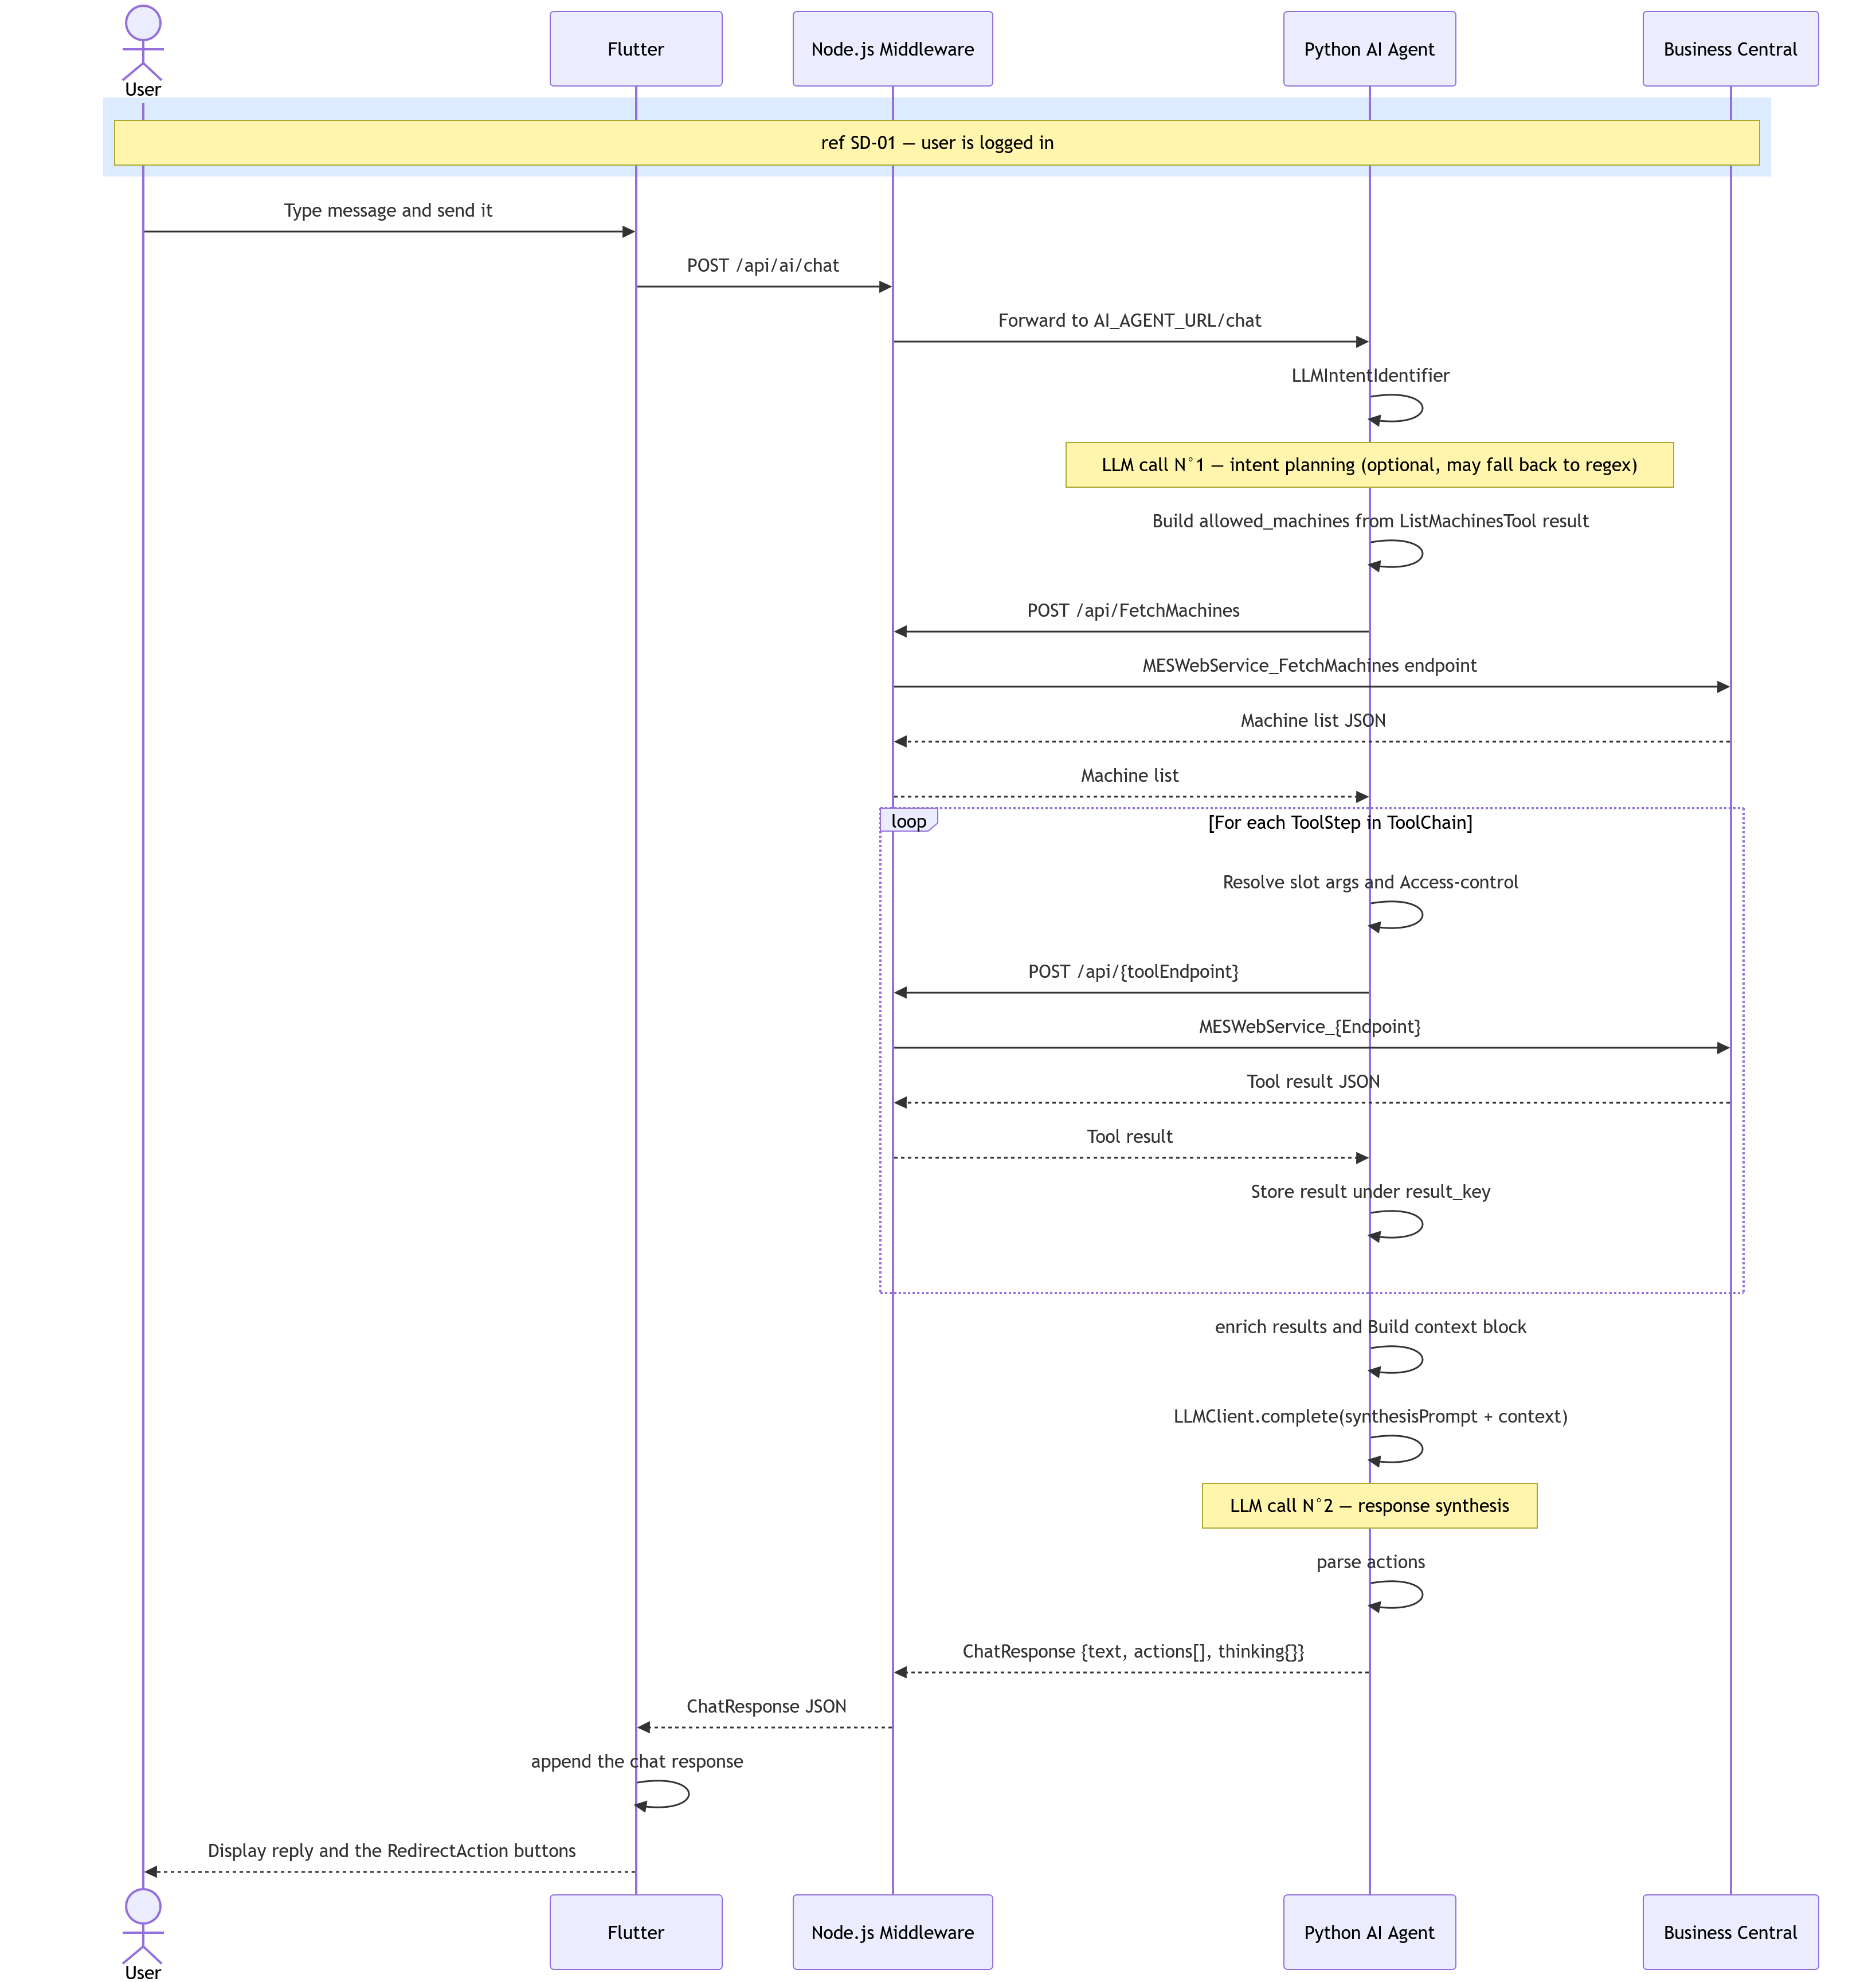
\includegraphics[width=\linewidth,height=0.82\textheight,keepaspectratio]{./media/MES_Sprint-5-Report/diagrams/sequence/AIChat-MainFlow.png}
  \caption{SD-30: AI Chat --- Main Flow.}
  \label{fig:s5-seq-ai-chat}
\end{figure}
%=====SD-30==========================================================
% sequenceDiagram
%     actor User
%     participant Flutter
%     participant Node as Node.js Middleware
%     participant Agent as Python AI Agent
%     participant BC as Business Central

%     rect rgb(220,235,255)
%         Note over User,BC: ref SD-01 — user is logged in
%     end

%     User->>Flutter: Type message and send it
%     Flutter->>Node: POST /api/ai/chat

%     Node->>Agent: Forward to AI_AGENT_URL/chat

%     Agent->>Agent: LLMIntentIdentifier
%     Note over Agent: LLM call N°1 — intent planning (optional, may fall back to regex)

%     Agent->>Agent: Build allowed_machines from ListMachinesTool result
%     Agent->>Node: POST /api/FetchMachines
%     Node->>BC: MESWebService_FetchMachines endpoint 
%     BC-->>Node: Machine list JSON
%     Node-->>Agent: Machine list

%     loop For each ToolStep in ToolChain
%         Agent->>Agent: Resolve slot args and Access-control
%         Agent->>Node: POST /api/{toolEndpoint}
%         Node->>BC: MESWebService_{Endpoint}
%         BC-->>Node: Tool result JSON
%         Node-->>Agent: Tool result
%         Agent->>Agent: Store result under result_key
%     end

%     Agent->>Agent: enrich results and Build context block

%     Agent->>Agent: LLMClient.complete(synthesisPrompt + context)
%     Note over Agent: LLM call N°2 — response synthesis

%     Agent->>Agent: parse actions
%     Agent-->>Node: ChatResponse {text, actions[], thinking{}}
%     Node-->>Flutter: ChatResponse JSON

%     Flutter->>Flutter: append the chat response
%     Flutter-->>User: Display reply and the RedirectAction buttons
%====================================================================

Figure~\ref{fig:s5-seq-intent-classification} illustrates the two-tier intent classification flow, showing the LLM-based primary classifier, the JSON plan validation step, and the fallback path to the regex classifier. The \domainterm{ThinkingBlock} capturing the classification trace is also shown.

\begin{figure}[H]
  \centering
  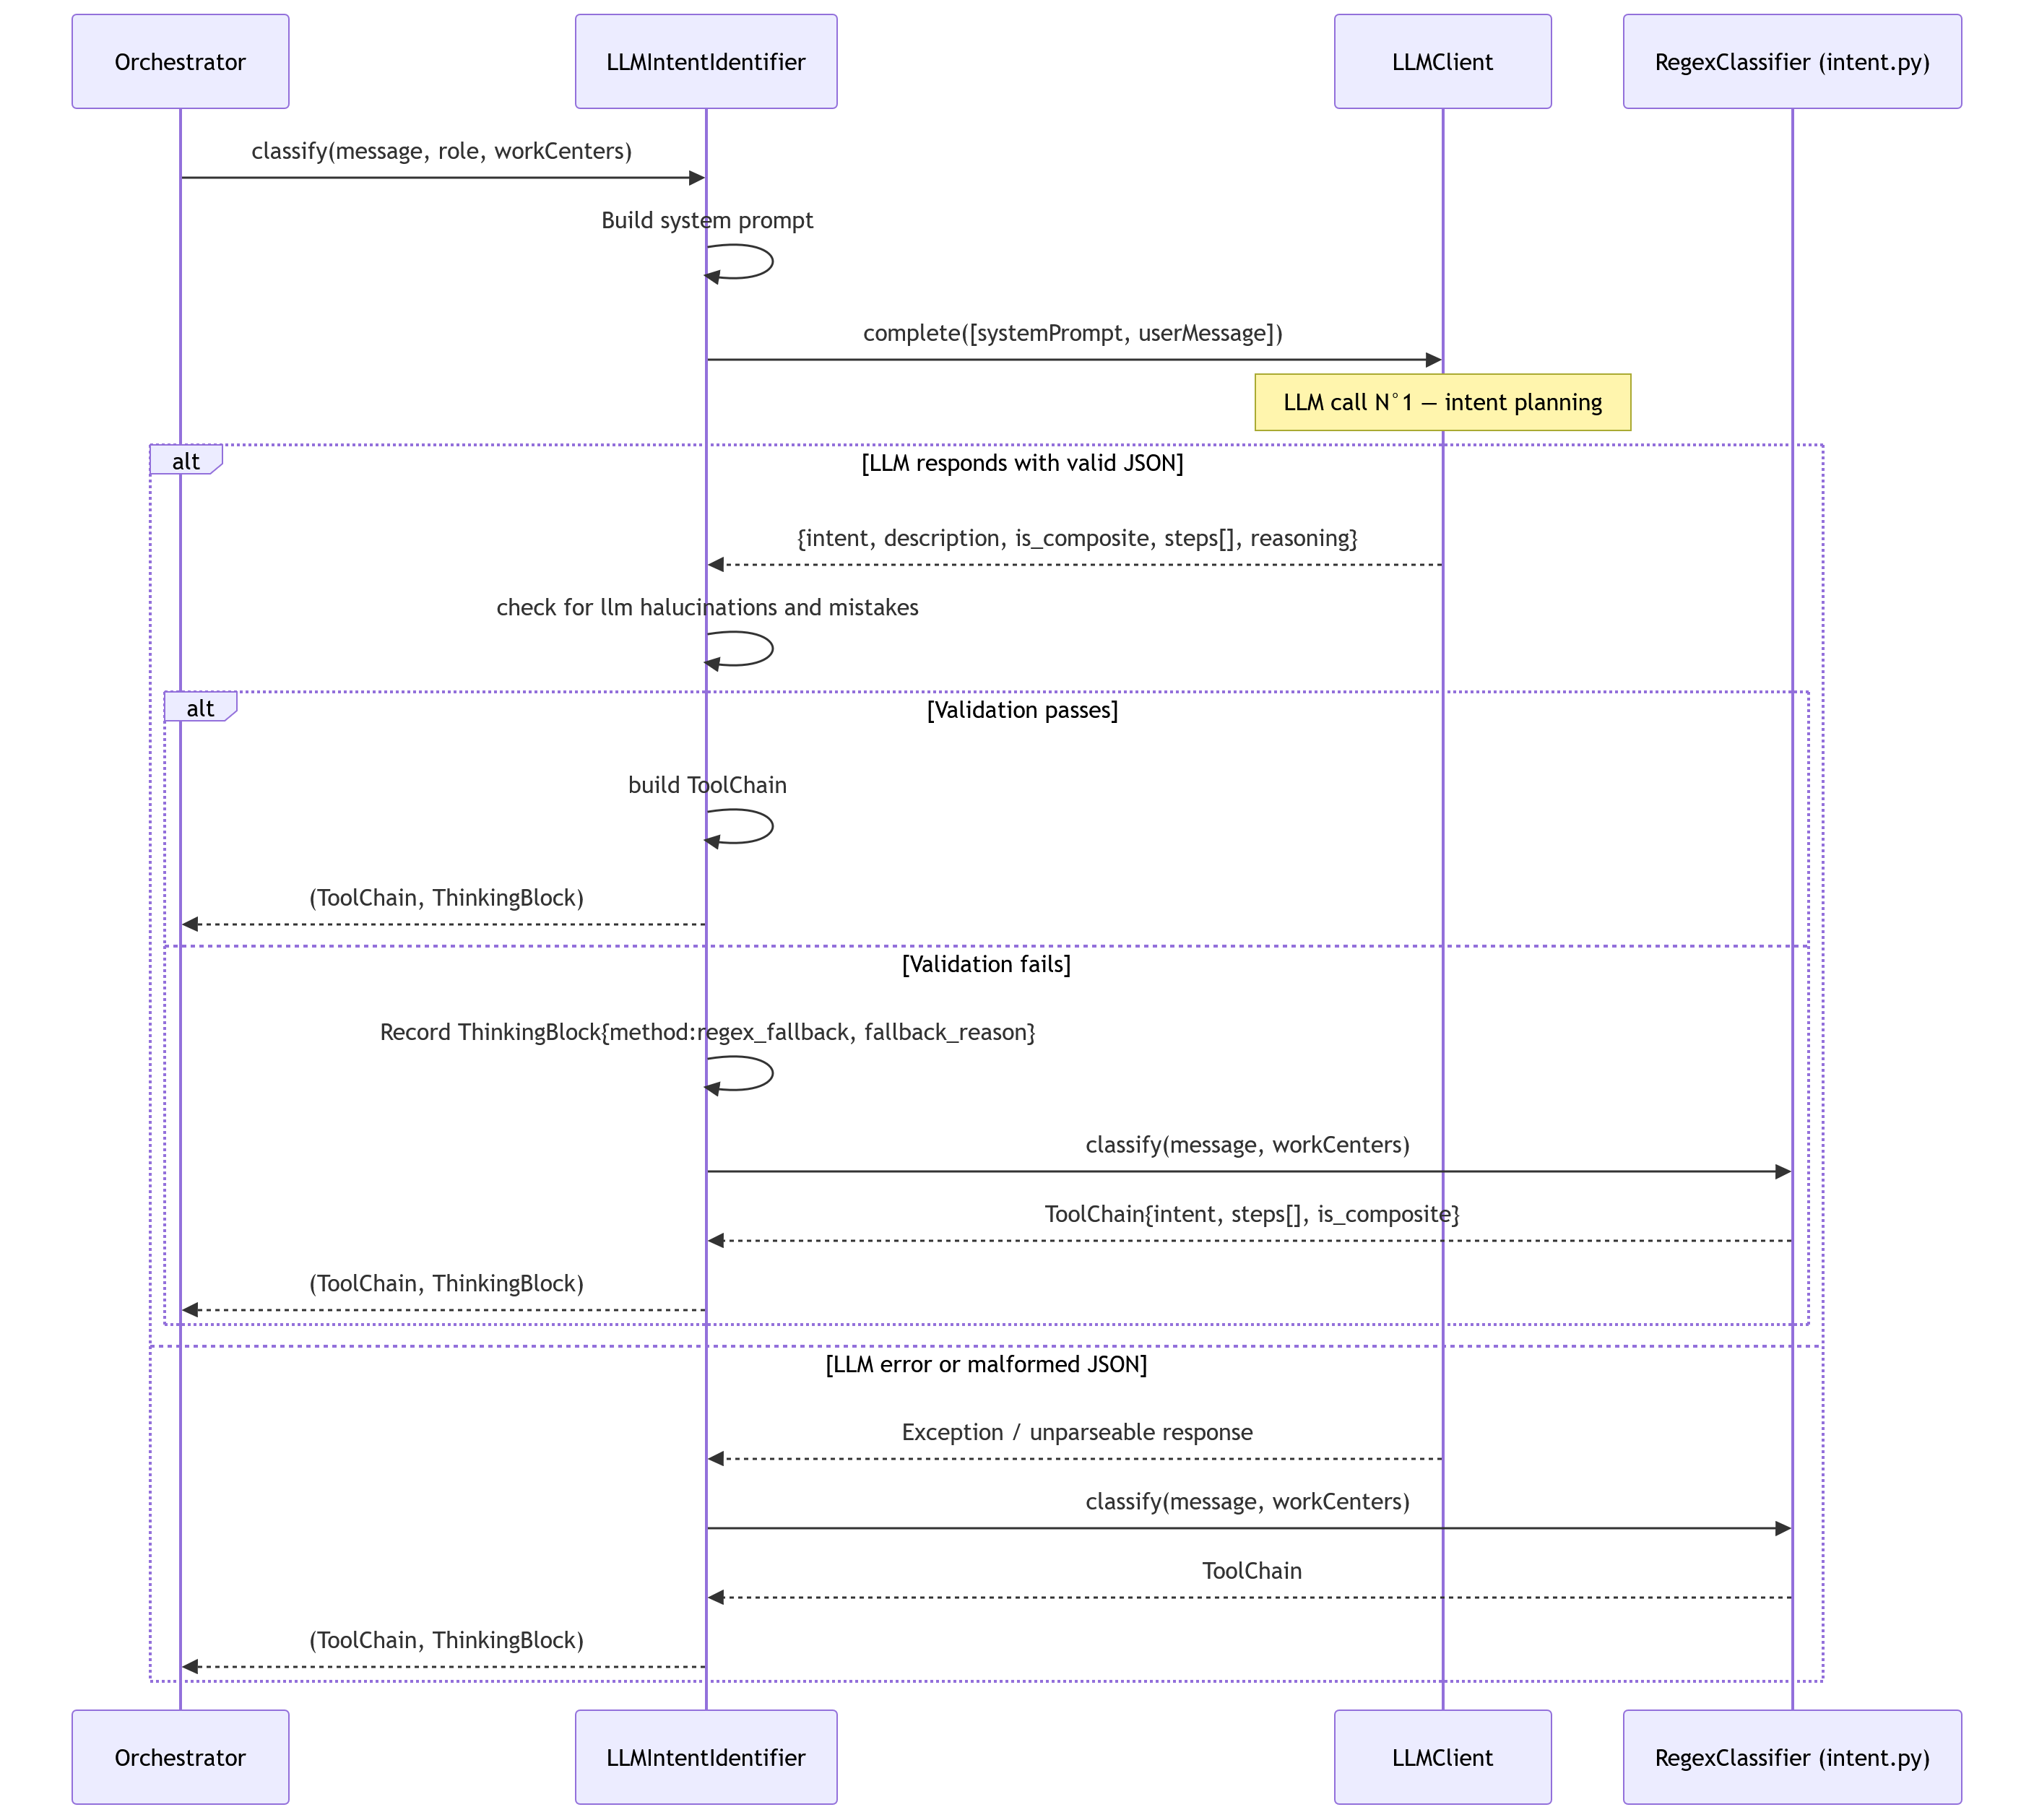
\includegraphics[width=\linewidth,height=0.82\textheight,keepaspectratio]{./media/MES_Sprint-5-Report/diagrams/sequence/Intent-Classification.png}
  \caption{SD-31: Intent Classification --- LLM with Regex Fallback.}
  \label{fig:s5-seq-intent-classification}
\end{figure}

% sequenceDiagram
%     participant Orch as Orchestrator
%     participant LLMIntent as LLMIntentIdentifier
%     participant LLMClient as LLMClient
%     participant Regex as RegexClassifier (intent.py)

%     Orch->>LLMIntent: classify(message, role, workCenters)

%     LLMIntent->>LLMIntent: Build system prompt
%     LLMIntent->>LLMClient: complete([systemPrompt, userMessage])
%     Note over LLMClient: LLM call N°1 — intent planning

%     alt LLM responds with valid JSON
%         LLMClient-->>LLMIntent: {intent, description, is_composite, steps[], reasoning}
%         LLMIntent->>LLMIntent: check for llm halucinations and mistakes
%         alt Validation passes
%             LLMIntent->>LLMIntent: build ToolChain
%             LLMIntent-->>Orch: (ToolChain, ThinkingBlock)
%         else Validation fails
%             LLMIntent->>LLMIntent: Record ThinkingBlock{method:regex_fallback, fallback_reason}
%             LLMIntent->>Regex: classify(message, workCenters)
%             Regex-->>LLMIntent: ToolChain{intent, steps[], is_composite}
%             LLMIntent-->>Orch: (ToolChain, ThinkingBlock)
%         end
%     else LLM error or malformed JSON
%         LLMClient-->>LLMIntent: Exception / unparseable response
%         LLMIntent->>Regex: classify(message, workCenters)
%         Regex-->>LLMIntent: ToolChain
%         LLMIntent-->>Orch: (ToolChain, ThinkingBlock)
%     end

\subsection{Class Diagram}

The UML Class Diagram (Figure~\ref{fig:s5-class-diagram-s5}) shows the Python AI agent's domain model. \modulename{MES Agent Orchestrator} is the central coordinator, holding references to an \modulename{LLM Intent Identifier}, an \modulename{LLM Client} (the abstract interface implemented by six concrete provider classes), and the \modulename{TOOL MAP} registry. \modulename{Tool Chain} is a value object produced by the classifiers and consumed by the orchestrator; it contains an ordered list of \modulename{Tool Step} records. All tool classes implement a common \texttt{execute()} interface. \modulename{Chat Request} and \modulename{Chat Response} are the inbound and outbound Pydantic contracts of the \texttt{/chat} endpoint.

\begin{figure}[H]
  \centering
  
\includegraphics[width=\linewidth,keepaspectratio]{./media/MES_Sprint-5-Report/placeholder-image.png}
  \caption{UML Class Diagram --- AI Assistant \& Analytical Intelligence.}
  \label{fig:s5-class-diagram-s5}
\end{figure}

% ---------------------------------------------------------------------------
% 4. IMPLEMENTATION
% ---------------------------------------------------------------------------
\section{Implementation}

\subsection{Python AI Agent}

\subsubsection{Data Models}

\begin{longtable}{@{} P{0.25\linewidth} P{0.25\linewidth} P{0.45\linewidth} @{}}
	\caption{Pydantic Models --- \modulename{agent/models.py}}
	\label{tab:s5-pydantic-models} \\
	\toprule
	\textbf{Class} & \textbf{Key Fields} & \textbf{Description} \\
	\midrule
	\endfirsthead
	\toprule
	\textbf{Class} & \textbf{Key Fields} & \textbf{Description} \\
	\midrule
	\endhead
	\multicolumn{3}{r}{\small Continued on next page} \\
	\endfoot
	\bottomrule
	\endlastfoot

	\techname{ConversationTurn} & \texttt{role}, \texttt{content} & One message in the conversation history. Role is either \texttt{"user"} or \texttt{"assistant"}. \\
	\midrule
	\techname{UserContext} & \texttt{user\_id}, \texttt{role}, \texttt{work\_centers}, \texttt{token} & Session identity extracted from the Flutter session storage and forwarded with every chat request. \\
	\midrule
	\techname{ChatRequest} & \texttt{message}, \texttt{user\_context}, \texttt{conversation\_history} & Inbound contract for the \texttt{POST /chat} endpoint. \texttt{conversation\_history} defaults to an empty list. \\
	\midrule
	\techname{ActionType} & enum: 5 values & Defines the five redirect types the LLM may emit: \texttt{redirect\_machine}, \texttt{redirect\_operation}, \texttt{redirect\_machine\_list}, and two reserved types. \\
	\midrule
	\techname{RedirectAction} & \texttt{action\_type}, \texttt{label}, \texttt{payload} & A clickable navigation action sent back to Flutter and rendered as an \texttt{ElevatedButton}. \\
	\midrule
	\techname{ChatResponse} & \texttt{text}, \texttt{actions}, \texttt{data\_fetched}, \texttt{thinking} & Outbound contract. \texttt{text} is the human-readable reply; \texttt{actions} holds up to 4 redirect actions; \texttt{thinking} carries the classification trace for debugging. \\
	\midrule
	\techname{ToolResult} & \texttt{tool\_name}, \texttt{success}, \texttt{data}, \texttt{error} & Internal result wrapper returned by every tool's \texttt{execute()} method. \\
\end{longtable}

\subsubsection{Intent Classification}

The intent classification layer comprises two components working in tandem. \modulename{llm\_intent.py} is the primary classifier: it sends a terse system prompt listing all 17 available tools to the configured LLM and expects a JSON response containing the \texttt{intent} label, a \texttt{steps} array, and an optional \texttt{reasoning} field. This plan is validated by \texttt{\_validate\_plan()}, which checks that the intent label is known, all tool names exist in \texttt{TOOL\_MAP}, and no \texttt{result\_key} is duplicated across steps.

If validation fails for any reason — malformed JSON, unknown tool, missing required field — control passes to \modulename{intent.py}, the deterministic regex classifier. Table~\ref{tab:s5-intent-classes} lists the 12 intent classes and their primary trigger patterns.

\begin{longtable}{@{} P{0.28\linewidth} P{0.67\linewidth} @{}}
	\caption{Intent Classes --- \modulename{agent/intent.py}}
	\label{tab:s5-intent-classes} \\
	\toprule
	\textbf{Intent} & \textbf{Primary Trigger Patterns} \\
	\midrule
	\endfirsthead
	\toprule
	\textbf{Intent} & \textbf{Primary Trigger Patterns} \\
	\midrule
	\endhead
	\multicolumn{2}{r}{\small Continued on next page} \\
	\endfoot
	\bottomrule
	\endlastfoot

	\texttt{BOM} & \textit{bom}, \textit{component}, \textit{material}, \textit{consumption}, \textit{scan} \\
	\midrule
	\texttt{PRODUCTION\_CYCLES} & \textit{cycle}, \textit{declaration}, \textit{declared}, \textit{production history} \\
	\midrule
	\texttt{OPERATION\_LIVE} & \textit{live}, \textit{current operation}, \textit{running}, \textit{in progress} \\
	\midrule
	\texttt{OPERATION\_HISTORY} & \textit{history}, \textit{past operation}, \textit{finished}, \textit{cancelled} \\
	\midrule
	\texttt{ORDERS} & \textit{order}, \textit{production order}, \textit{PO-}, \textit{scheduled} \\
	\midrule
	\texttt{MACHINE\_LIVE} & \textit{machine status}, \textit{what is MC-}, \textit{ongoing} \\
	\midrule
	\texttt{DASHBOARD} & \textit{dashboard}, \textit{summary}, \textit{overview}, \textit{KPI} \\
	\midrule
	\texttt{MACHINE\_STATUS} & \textit{idle}, \textit{working}, \textit{which machines are} \\
	\midrule
	\texttt{SCRAP\_ANALYSIS} & \textit{scrap}, \textit{reject}, \textit{waste}, \textit{defect} \\
	\midrule
	\texttt{ACTIVITY} & \textit{activity}, \textit{event log}, \textit{what happened}, \textit{recent actions} \\
	\midrule
	\texttt{DEPARTMENT} & \textit{work center}, \textit{department}, \textit{sector}, \textit{operator summary} \\
	\midrule
	\texttt{GENERAL} & Catch-all when no higher-priority rule matches. \\
\end{longtable}

\subsubsection{Tool Catalogue}

Table~\ref{tab:s5-tool-catalogue} lists all 17 tool classes registered in \texttt{TOOL\_MAP}, together with the \techname{Business Central} endpoint each tool calls and its primary arguments.

\begin{longtable}{@{} P{0.32\linewidth} P{0.30\linewidth} P{0.33\linewidth} @{}}
	\caption{MES Tool Catalogue --- \modulename{tools/mes\_tools.py}}
	\label{tab:s5-tool-catalogue} \\
	\toprule
	\textbf{Tool Class} & \textbf{BC Endpoint} & \textbf{Key Arguments} \\
	\midrule
	\endfirsthead
	\toprule
	\textbf{Tool Class} & \textbf{BC Endpoint} & \textbf{Key Arguments} \\
	\midrule
	\endhead
	\multicolumn{3}{r}{\small Continued on next page} \\
	\endfoot
	\bottomrule
	\endlastfoot

	\techname{ListMachinesTool} & \texttt{FetchMachines} & \texttt{work\_center\_no} \\
	\midrule
	\techname{GetMachineOrdersTool} & \texttt{getMachineOrders} & \texttt{machine\_no} \\
	\midrule
	\techname{GetOngoingOperationsTool} & \texttt{fetchOngoing-\linebreak OperationsState} & \texttt{machine\_no} \\
	\midrule
	\techname{GetOperationLiveDataTool} & \texttt{fetchOperationLiveData} & \texttt{machine\_no}, \texttt{prod\_order\_no}, \texttt{operation\_no} \\
	\midrule
	\techname{GetProductionCyclesTool} & \texttt{fetchProductionCycles} & \texttt{machine\_no}, \texttt{prod\_order\_no}, \texttt{operation\_no} \\
	\midrule
	\techname{GetOperationsHistoryTool} & \texttt{fetchOperationsHistory} & \texttt{machine\_no} \\
	\midrule
	\techname{GetActivityLogTool} & \texttt{fetchActivityLog} & \texttt{hours\_back} \\
	\midrule
	\techname{GetMachineDashboardTool} & \texttt{fetchMachineDashboard} & \texttt{hours\_back}, \texttt{work\_center\_nos} \\
	\midrule
	\techname{GetProductionOrdersTool} & \texttt{fetchProductionOrders} & \texttt{status\_filter}, \texttt{work\_center\_no}, \texttt{machine\_no} \\
	\midrule
	\techname{GetWorkCenterSummaryTool} & \texttt{fetchWorkCenterSummary} & \texttt{work\_center\_nos}, \texttt{hours\_back} \\
	\midrule
	\techname{GetOperatorSummaryTool} & \texttt{fetchOperatorSummary} & \texttt{work\_center\_nos}, \texttt{hours\_back} \\
	\midrule
	\techname{GetMyDataTool} & \texttt{fetchMyData} & \texttt{hours\_back} (token-scoped) \\
	\midrule
	\techname{GetScrapSummaryTool} & \texttt{fetchScrapSummary} & \texttt{hours\_back}, multi-filter \\
	\midrule
	\techname{GetDelayReportTool} & \texttt{fetchDelayReport} & \texttt{work\_center\_nos}, \texttt{pause\_threshold\_minutes} \\
	\midrule
	\techname{GetConsumptionSummaryTool} & \texttt{fetchConsumptionSummary} & \texttt{prod\_order\_no}, \texttt{operation\_no}, \texttt{machine\_no}, \texttt{hours\_back} \\
	\midrule
	\techname{GetSupervisorOverviewTool} & \texttt{fetchSupervisorOverview} & \texttt{work\_center\_nos}, \texttt{hours\_back}, \texttt{pause\_threshold\_minutes} \\
	\midrule
	\techname{GetBomTool} & \texttt{fetchBom} & \texttt{prod\_order\_no}, \texttt{operation\_no} \\
\end{longtable}

\subsubsection{Orchestration Pipeline}

\techname{MESAgentOrchestrator.run()} processes each \texttt{ChatRequest} through an eight-step pipeline. Step 1 calls \texttt{LLMIntentIdentifier.classify()} (with regex fallback) to produce a \texttt{ToolChain}. Step 2 routes to the composite path (if \texttt{is\_composite = true}) or the normal sequential path. Step 3 resolves any \texttt{unresolved\_machine\_ref} using \modulename{resolver.py}. Step 4 iterates the tool steps: slot arguments prefixed with \texttt{\$} are resolved against prior step results, access-control is verified against \texttt{allowed\_machines}, and the tool is executed. Step 5 applies \modulename{data\_analysis.py} enrichment per result key. Step 6 assembles the LLM context block and truncates it to \texttt{LLM\_MAX\_CONTEXT\_CHARS}. Step 7 calls the LLM once for synthesis. Step 8 extracts any \texttt{```actions```} block from the reply and separates it from the displayed text.

\subsubsection{Multi-Provider LLM Client}

The \texttt{build\_llm\_client()} factory reads the \texttt{LLM\_PROVIDER} environment variable and instantiates the corresponding client class. All clients expose the same \texttt{async complete(messages: list) → str} interface so the rest of the agent is provider-agnostic. Table~\ref{tab:s5-llm-providers} summarises the supported providers.

\begin{longtable}{@{} P{0.30\linewidth} P{0.30\linewidth} P{0.35\linewidth} @{}}
	\caption{Supported LLM Providers --- \modulename{agent/llm\_client.py}}
	\label{tab:s5-llm-providers} \\
	\toprule
	\textbf{Client Class} & \textbf{Provider} & \textbf{Notes} \\
	\midrule
	\endfirsthead
	\toprule
	\textbf{Client Class} & \textbf{Provider} & \textbf{Notes} \\
	\midrule
	\endhead
	\multicolumn{3}{r}{\small Continued on next page} \\
	\endfoot
	\bottomrule
	\endlastfoot

	\techname{OllamaClient} & Local Ollama & No external credential required; model served locally. \\
	\midrule
	\techname{OpenAIClient} & OpenAI & Requires \texttt{OPENAI\_API\_KEY}. \\
	\midrule
	\techname{HuggingFaceClient} & HF Serverless Inference & Requires \texttt{HF\_API\_TOKEN}. \\
	\midrule
	\techname{OpenAICompatibleClient} & Groq, Together, Mistral, vLLM, LM Studio & Uses the OpenAI Chat Completions schema with a configurable base URL. \\
	\midrule
	\techname{AnthropicClient} & Anthropic & Extracts the system prompt from the messages list before calling the Messages API. \\
\end{longtable}

\subsection{Node.js Middleware}

\subsubsection{Endpoint Routing}

We configured the middleware to map all calls coming from the frontend using the structure \techname{/api/ai} to the ai proxy handler which forwards them to the \techname{/chat} endpoint of the Python agent. The agents tool calls are treated through the same path as the normal business central function calls by the flutter frontend.

\subsection{Flutter Frontend}

\subsubsection{AI Data Layer}

The Flutter data layer for the AI feature comprises three classes. \techname{AiChatService} constructs the full request payload — including user context assembled from \techname{SessionStorage} at call time — and POSTs it to \apiendpoint{/api/ai/chat}. It deserialises the response into an \techname{AiChatResponse} object. \techname{ConversationTurn} is a minimal data class with \texttt{role} and \texttt{content} fields and a \texttt{toJson()} serialiser. \techname{AiChatResponse} holds the reply text, the list of \techname{AiRedirectAction} objects, and an optional error string.

\subsubsection{AI Domain Layer}

\techname{AiChatProvider} extends \texttt{ChangeNotifier} and owns the conversation history as a \texttt{List\linebreak<ConversationTurn>}. Its \texttt{sendMessage()} method appends the user turn before calling the service, and on success appends the assistant turn and stores \texttt{lastResponse}. On failure it removes the failed user turn and sets \texttt{errorMessage}. \texttt{clearHistory()} resets both the history and the last response, enabling the user to start a fresh conversation.

\subsubsection{User Interface}

Figure~\ref{fig:s5-ui-ai-chat-mobile} illustrate the \uilabel{AI Chat} interface in its two display modes. On desktop (width $\geq$ 600 px), the chat panel opens as a 400 px fixed-width side panel anchored to the right of the \uilabel{Machine List Page}, and the floating action button (FAB) is hidden while the panel is open. On mobile, the chat opens as a full \texttt{Dialog} widget (max 800$\times$800 px). In both modes the interface comprises the same four sub-widgets: \techname{\_EmptyState} (shown before the first message), \techname{\_MessageBubble} (dark background for user turns, light grey for assistant turns, capped at 78\% of available width), \techname{\_ActionButtons} (a \texttt{Wrap} of \texttt{ElevatedButton}s for each \techname{RedirectAction}), and \techname{\_InputBar} (a \texttt{TextField} with a send icon button that switches to a \texttt{CircularProgressIndicator} while a request is in flight).
% empty state
\begin{figure}[H]
  \centering
  
\includegraphics[width=0.5\linewidth,keepaspectratio]{./media/MES_Sprint-5-Report/placeholder-image.png}
  \caption{\uilabel{AI Chat} dialog --- mobile view.}
  \label{fig:s5-ui-ai-chat-mobile-empty}
\end{figure}


% message state don't forget to add a redirect action
\begin{figure}[H]
  \centering
  
\includegraphics[width=0.5\linewidth,keepaspectratio]{./media/MES_Sprint-5-Report/placeholder-image.png}
  \caption{\uilabel{AI Chat} dialog --- mobile view.}
  \label{fig:s5-ui-ai-chat-mobile}
\end{figure}

% ---------------------------------------------------------------------------
% CONCLUSION
% ---------------------------------------------------------------------------
\phantomsection
\section*{Conclusion}
\addcontentsline{toc}{section}{Conclusion}

This sprint delivered the complete AI intelligence layer of the MES system. Operators and supervisors can now query production data, machine status, scrap rates, BOM consumption, operator performance, and shift overviews using natural language through the embedded chat assistant. The two-tier intent classification architecture — LLM-based planning with deterministic regex fallback — ensures reliable and responsive behaviour regardless of LLM availability. Work-centre-scoped access control, implemented entirely in Python and independent of LLM output, guarantees that users can only query data within their authorised scope. The multi-provider LLM client makes the system adaptable to different deployment environments, from a locally-hosted Ollama model to cloud providers such as Anthropic or OpenAI. The \techname{Node.js} middleware resolves the SSPI authentication challenge inherent to \techname{Business Central}'s OData layer while keeping the Flutter client and Python agent free of Windows-specific dependencies. Together, these components form a production-ready conversational intelligence layer that integrates seamlessly with the shop-floor execution features delivered in the preceding sprints.


%% CHAPTERS:END


% ---------------------------------------------------------------------------
% GENERAL CONCLUSION
% ---------------------------------------------------------------------------
\chapter*{General Conclusion}
\addstarredchapter{General Conclusion}
\markboth{General Conclusion}{}

This report has presented the full lifecycle of the MES (\textit{Manufacturing
Execution System}) project developed at \textbf{\CompanyName{}} over the course
of five sprints. Starting from a blank slate, the team designed and implemented
a complete shop-floor execution system natively integrated with Microsoft
Dynamics 365 Business Central.
Sprint~1 established the security and identity foundation: a token-based
authentication system, role-based access control, and a full administrator
interface for user and account management. Sprint~2 delivered real-time machine
monitoring, production order management, and a complete operation history trail.
Sprint~3 completed the production execution loop with declarations, pause,
resume, finish, and close flows, Bill of Materials visibility, component scanning, scrap
tracking, and label printing. Sprint~4 added a
machine performance dashboard, a paginated activity log for the Administrator, multi-language support
covering English, French, and Arabic, and in-app onboarding tutorials.
Sprint~5 delivered the AI intelligence layer: a natural-language chat assistant
embedded in the Flutter frontend, a Node.js reverse-proxy middleware bridging
the Flutter application to both Business Central and a Python AI agent, and the
agent itself, providing intent classification, multi-provider LLM synthesis,
fuzzy machine resolution, composite fan-out queries, and contextual redirect
actions.
Across all five sprints, the append-only data model ensures a tamper-evident
audit trail from every machine state change through to every production cycle
declaration. The reactive stream architecture in the Flutter frontend provides
operators and supervisors with a consistent, real-time view of the production
floor without manual refreshes.
The project demonstrates that a tightly integrated MES solution can be built
on top of Microsoft Dynamics 365 Business Central~\cite{businesscentral} using OData V4 unbound
actions, with a Node.js middleware layer handling Windows authentication and
AI routing. The extensible layered architecture positions the system for future
enhancements such as statistical reporting, alert management, and additional
language support.

% ---------------------------------------------------------------------------
% BIBLIOGRAPHY
% ---------------------------------------------------------------------------
% ── Webography ────────────────────────────────────────────────────────────────
{
  \setlength{\cftbeforelottitleskip}{0pt}
  \setlength{\cftafterlottitleskip}{10pt}
  \renewcommand{\bibname}{Webography}
  \begin{thebibliography}{9}
  %% BIBLIOGRAPHY:BEGIN 
  % -- auto-merged bibliography entries --
  \bibitem{mavision}
      MAVISION, \textit{Official Website}, \url{https://www.mavision.tn},
      visited April 2025. 
    \bibitem{dassault_apriso}
      Dassault Syst\`{e}mes,\textit{DELMIA Apriso --- Manufacturing Operations Management},
      \url{https://www.3ds.com/products/delmia/apriso}, visited April 2025. 
    \bibitem{agilemanifesto}
      K.~Beck \textit{et~al.},
      \textit{Manifesto for Agile Software Development}, 2001.
      \url{https://agilemanifesto.org}, visited April 2025.    
    \bibitem{scrumguide}
      K.~Schwaber and J.~Sutherland,
      \textit{The Scrum Guide},
      Scrum.org, November 2020.
      \url{https://scrumguides.org/scrum-guide.html}, visited April 2025.
  \bibitem{nodejs}
      OpenJS Foundation,
      \textit{Node.js --- JavaScript Runtime Built on Chrome's V8 Engine},
      \url{https://nodejs.org}, visited April 2025. 
    \bibitem{express}
      OpenJS Foundation,
      \textit{Express 5.x --- Fast, Unopinionated, Minimalist Web Framework for Node.js},
      \url{https://expressjs.com}, visited April 2025.   
    \bibitem{flutter}
      Google LLC,
      \textit{Flutter --- Build Apps for Any Screen},
      \url{https://flutter.dev}, visited April 2025.   
    \bibitem{fastapi}
      S.~Ram\'{\i}rez,
      \textit{FastAPI --- Modern, Fast Web Framework for Building APIs with Python},
      \url{https://fastapi.tiangolo.com}, visited April 2025.
    \bibitem{python}
      Python Software Foundation,
      \textit{Python Programming Language},
      \url{https://www.python.org}, visited April 2025.
    \bibitem{businesscentral}
      Microsoft Corporation,
      \textit{Microsoft Dynamics~365 Business Central Documentation},
      \url{https://learn.microsoft.com/en-us/dynamics365/business-central/},
      visited April 2025.
    \bibitem{dart_lang}
      Google LLC,
      \textit{Dart Programming Language},
      \url{https://dart.dev}, visited April 2025.
    \bibitem{postman}
      Postman Inc.,
      \textit{Postman --- API Platform for Building and Using APIs},
      \url{https://www.postman.com}, visited April 2025.
    \bibitem{ollama}
      Ollama,
      \textit{Ollama --- Get Up and Running with Large Language Models Locally},
      \url{https://ollama.ai}, visited April 2025.
    \bibitem{openai_api}
      OpenAI,
      \textit{OpenAI API Reference},
      \url{https://platform.openai.com/docs/api-reference}, visited April 2025.
    \bibitem{anthropic}
      Anthropic,
      \textit{Anthropic --- AI Safety Company},
      \url{https://www.anthropic.com}, visited April 2025.
  %% BIBLIOGRAPHY:END
  \end{thebibliography}
}
\end{document}
